
%\qquad Due quadratoni.
%
%\quad Un quadratone.
%
%\<SP> Uno spazio «normale».
%
%$\;$  Uno spazio spesso (5/8 di quadratone).
%
%$\>$  Uno spazio medio (2/9 di quadratone).
%
%$\.$  Uno spazio molto sottile (1/6 di quadratone).
%
%$\!$  Uno spazio negativo (-1/6 di quadratone).



%\documentclass[11 pt , letterpaper , twoside , openright ]{book}
\documentclass[11 pt , A4 , oneside ]{book}
\usepackage[T1]{fontenc}
\usepackage[utf8]{inputenc}
\usepackage{etoolbox}

\usepackage[ED=MEGEP-DyF, Ets=INP]{tlsflyleaf}


\usepackage[english]{babel}

\usepackage{caption} 
%\usepackage{subfig}

\usepackage{transparent}
\usepackage{eso-pic}
\usepackage{textcomp}
%\usepackage[acronym]{glossaries}

\usepackage{url} %generare collegamenti

\newcommand{\chapquote}[3]{\begin{quotation} \textit{#1} \end{quotation} \begin{flushright} - #2, \textit{#3}\end{flushright} } %writes quotes as chapter beginning

%%%%%%%%%%%%%%%%%%%%%%%%%%%%%%%%%%%%%%%%%%%%%%%%%%%%%%%

\usepackage{graphicx}
\usepackage{epsfig}
\usepackage{psfrag}
%\usepackage{subfigure}
\usepackage{subcaption}
% AMS bundle

\usepackage{amssymb}
\usepackage{amsmath}
\usepackage{amsfonts}
\usepackage{amsbsy}
\usepackage{amsthm}

\usepackage{bm}
\usepackage{epsfig}
\usepackage{epstopdf}
\usepackage{color}

\usepackage{caption}
\usepackage{booktabs}
\usepackage{float} % is needed by \begin{figure}[H]  to write [H]
\usepackage{mathrsfs}

\usepackage[linesnumbered]{algorithm2e}  %writing pseudocode

\usepackage{minted} % writing code snippets
%\usemintedstyle{emacs}


\usepackage[numbers, square]{natbib}
%%%%%%%%%%%%%%%%%%%%%%%%%%%%%%%%%%%%%%%%%%%%%%%%%%%%%%%

\newtheorem{theorem}{Theorem}[]
\newtheorem{corollary}{Corollary}[]

\newcommand{\bs}[1]{\boldsymbol{#1}}

\newcommand{\derp}[2]{\dfrac{\partial #1}{\partial #2}}

\def\rprth#1{\left( #1 \right)} %\prth{.} inside round parentesis
\def\sprth#1{\left[ #1 \right]} %\prth{.} inside square parentesis
\def\gprth#1{\left{ #1 \right}} %\prth{.} inside graph parentesis
\newcommand{\volb}{V_\beta} %\volb  volume of the fluid phase
\def\meani#1{{\left< #1 \right>}^{\beta}} %\mean{.} intrinsic average operator
\def\means#1{{\left< #1 \right>}} %\mean{.} superficial average operator
\newcommand{\vb}{\textbf{v}_{\beta}} %\vb velocity in the fluid
\newcommand{\ws}{\textbf{v}_{\sigma}} %\vb velocity in the fluid
\newcommand{\vbt}{\tilde{\textbf{v}}_{\beta}} %\vb velocity in the fluid
\newcommand{\pbt}{\tilde{p}_{\beta}} %\pbt spatial fluctuation pressure in the fluid
\newcommand{\vbmi}{\meani{\textbf{v}_{\beta}}} %\vbmi intrinsic average velocity of fluid phase 
\newcommand{\vbms}{\means{\textbf{v}_{\beta}}} %\vbms superficial average velocity of fluid phase 
\newcommand{\rhos}{\rho_{\sigma}} %\ density of the solid phase
\newcommand{\pb}{p_{\beta}} %\pb pressure of fluid phase
\newcommand{\pbmi}{\meani{p_{\beta}}} %\pbmi intrinsic average pressure of fluid phase 
\newcommand{\pbms}{\means{\textbf{v}_{\beta}}} %\vbms superficial average velocity of fluid phase 
\newcommand{\nub}{\nu_{\beta}} %\nub cinematic viscosity of fluid phase
\newcommand{\mub}{\mu_{\beta}} %\mub dynamic viscosity of fluid phase
\newcommand{\nbs}{\mathbf{n}_{\beta \sigma }} %\mub dynamic viscosity of fluid phase

\newcommand{\Red}[1]{{\textcolor{red}{#1}}}
\newcommand{\Blue}[1]{{\textcolor{blue}{#1}}}

\newcommand{\vs}[1]{\vspace{ #1 cm}}
\newcommand{\hs}[1]{\hspace{ #1 cm}}

%%%%%%%%%%%%%%%%%%%%%%%%%%%%%%%%%%%%%%%%%%%%%%%%%%%%%%%

\input frontpage

%%%%%%%%%%%%%%%%%%%%%%%%%%%%%%%%%%%%%%%%%%%%%%%%%%%%%%%
% with this you compile only one chapter and not the all document
% \includeonly{appendix_a/appendix_a}
%%%%%%%%%%%%%%%%%%%%%%%%%%%%%%%%%%%%%%%%%%%%%%%%%%%%%%%





\begin{document}
	\makeflyleaf


%\include{contorno/dediche}
\chapter*{Abstract}

Almost all the surfaces existing in Nature are not at all smooth, they present a more or less regular arrangement of rugosities and/or solid structures at various length scales.
The effectiveness of these surfaces in increasing the aerodynamic performances (drag reduction, lift enhancement, separation control…) has been proved in numerous cases such as boundary layers and bluff bodies.
The microscopic computation of the flow around such multi-scale surfaces is practically unfeasible, so the ideas that we want to exploit in this work is to find a way to model the apparent slip over these surfaces (modeled as porous layers) using the Volume-Average theory \citet{whitaker2013method}.
This mathematical method allows to average out the details of the micro-scale structures on such surfaces and still have a good description of the phenomenon involved.
The first chapter of this manuscript gives a panoramic of the previous efforts in the modellization of such surfaces, and present the main indication that we can extract from the results in literature.
The second chapter presents the mathematical derivation of the Volume-Averaged Navier-Stokes equation (VANS) for a flow over and through a porous medium saturated by a fluid.
In the third chapter we study the stability of the flow over the interface of a free fluid and a porous media, made of an array of rigid cylindrical pillars.
The presence of such porous layer has been treated adding a drag term in the fluid equations. 
We show that this term reduces the amplification factor of the Kelvin-Helmholtz instability throughout the whole range of wave-numbers and increases slightly the wavelength of the fastest growing mode.
In the same context we have computed the difference between the isotropic drag model and the tensorial approach for the drag term, in order to understand which is the most robust approach for stability computations; concluding that the tensorial approach, that use the apparent permeability tensor, is the best choice.
Based on this result, in chapter four we have computed numerically the apparent permeability tensor for a 3D porous medium constituted by rigid cylinder, by means of the closure problems arising from the VANS equations. Such a tensor varies with the Reynolds number, the mean pressure gradient orientation and the porosity. A database has been created to explore the space of the above parameters. The two Euler angles that define the mean pressure gradient orientation are included in order to well capture possible 3D effects. Based on the database, a kriging interpolation metamodel is used to obtain an estimate of all the tensor components for any input parameters. 
In the last chapter we show some results based on the metamodel; the use of such a reduced order model together with a numerical code based on the VANS equations at the macroscopic scale permits to maintain the computational times within reasonable levels.
To validate the macroscopic description we compare the VANS computation, of a closed cavity flow with a porous bottom layer, against the DNS results homogenized a posteriori. The comparison shows that there is a good agreement between the two models.
Using the same macroscopic description we further exploit the possibility of using the VANS model in order to compute the effectiveness of such porous layer to passively control flow separation in some classical geometry.
The last chapter includes the main conclusion of the work and the possible research direction to further develop the topic.

\chapter*{Résumé}

Toute surface naturelle est par essence non lisse, elle est constituée de rugosités plus ou moins régulières et / ou de structures mobiles d’échelles variées. D’un point de vue mécanique des fluides, ces surfaces naturelles proposent des meilleures performances aérodynamiques en termes de réduction de traînée, d’augmentation de la portance ou de contrôle du décollement lorsqu’elles couvrent des corps en mouvement. Cela a été notament prouvé pour des écoulements de couches limites ou de sillage, autour de corps épais. La simulation numérique d’écoulements aux échelles microscopiques autour des surfaces « naturelles » demeure de nos jours encore hors de portée. En conséquence, la thèse a pour objet d’étudier la modélisation du glissement apparent de l’écoulement sur ce genre de surface, modélisée comme un milieu poreux, appliquant la théorie de la moyenne-volumique de Whitaker. Ce modèle mathématique permet globalement de représenter en moyenne les détails de la micro-structure de ses surfaces, tout en conservant une description satisfaisante des phénomènes physiques induits par l’écoulement. 
Le premier chapitre de ce manuscrit dresse un panorama des efforts antérieurs portant sur la modélisation de ces surfaces en précisant les résultats les plus importants issus de la littérature. Le deuxième chapitre présente la dérivation mathématique des équations de Navier-Stokes en moyenne volumique (VANS en anglais) dans un milieu poreux. Dans le troisième chapitre est étudiée la stabilité de l’écoulement à l’interface entre un fluide libre et un milieu poreux, constitué d'une série de cylindres rigides. La présence de cette couche poreuse est traitée par un terme de traînée dans les équations du fluide. On montre que l'ajout de ce terme réduit les taux d’amplification de l’instabilité de Kelvin-Helmholtz sur toute la gamme des nombre d’onde et ainsi augmente la longueur d’onde du mode le plus amplifié. Dans ce même contexte a été calculée la différence entre un modèle isotrope et une approche tensorielle pour le terme de traînée, afin de déterminer l’approche la plus consistante pour une étude de stabilité de ce type d’écoulement. Cela a mené à la conclusion que le modèle le plus pertinent est celui utilisant le tenseur de perméabilité apparent. Dans le chapitre suivant le tenseur de perméabilité apparent est identifié sur la base d’une centaine de simulations numériques directes, pour un milieu poreux tridimensionnel constitué de cylindres rigides, où le problème de fermeture est abordé par la méthode VANS. Dans ces configurations ce tenseur varie en fonction de quatre paramètres : le nombre de Reynolds, la porosité et l’orientation du gradient moyen de pression définie par deux angles d’Euler. Cette paramétrisation permet de capturer les effets tridimensionnels locaux. Cette base de données ainsi constituée a permis de créer, une approche de type kriging, un métamodèle comportemental pour estimer toutes les composantes du tenseur de perméabilité apparente.


Dans le cinquième chapitre sont menées des simulations des équations VANS à l’échelle macroscopique après implémentation du méta-modèle qui autorise des temps de calcul raisonnables.  La validation de l’approche à l’échelle macroscopique est effectuée sur un écoulement dans une cavité fermé couverte d’une couche poreuse et une comparaison avec les résultats d’un DNS très précise, homogénéisés a posteriori montre un très bon accord et démontre la pertinence de la démarche. L’étape suivante a consisté en l’étude du contrôle du décollement pour un écoulement autour d’une bosse poreuse par cette même approche VANS macroscopique. Enfin des conclusions générales et des directions de recherche possibles sont présentées dans le dernier chapitre.
%%\include{contorno/nomenclatura}

\tableofcontents


\chapter{Poroelastic natural coatings}

\section{Biomimetics of poroelastic coatings}

Usually when someone is asked to imagine some "rapid" object as an airplane, a boat or a car, the common sense lead us to think about it as the smoothest as possible and most of the time shiny.
But if we look around us the nature seems not to agree with the previous statement.
In fact most of the surfaces in nature are not smooth at all, they present almost always some kind more or less regular arrangement of discontinuities at various length scales.
Since Nature have had a very large time-span to optimize this kind of surfaces we can be very certain that they are the best possible option.
One should pinpoint that the non smoothness of these surfaces can be connected to some other biological functions rather than pure fluid dynamic performance, and of course it can be the case.


With that in mind we want to show to the reader some of the most notably examples of "natural" aerodynamically surfaces.

Probably the most notable example is the shark skin, in figure \ref{fig:shark} a segment of the skin is depicted as if appears to be under the microscope.

\begin{figure}[h]
	\centering
	\includegraphics[width=0.6\linewidth]{chapter_1/shark}
	\caption{Microscope enlarged picture of the shark skin.}
	\label{fig:shark}
\end{figure}

The enlargement show that the surface is made up by a series of overlapped denticles, and experiment shows that they can move and interact with the flow.

The shark technology has somehow been applied by Speedo$^{\circledR}$ in their famous swimming suits, that had break multiples world records.
But it seems that this controversial swimmers performance came more on the compressed and streamlined body shape than from the surface texture itself.
In fact during the years this texture material has been publicized to be like synthetic shark skin but \cite{Oeffner785} has shown that the texture is somehow different from the shark dermal structure.
They have also performed some swimming experiment with a flat plate with different surfaces and they have found no significant speed enhancement with the swimsuit surfaces; but the measurements with the shark skin on the contrary give an appreciable improvement in the performance.


Poroelastic surfaces find also applications in aeroacoustics, in fact the owl is well known for its particularly silent flight, in the high frequency spectrum.
This characteristic is crucial for the owl in order to be able to capture his preys.
Obviously it has inspired the scientific community to study the feathers configuration and their shape.

\begin{figure}[h]
	\centering
	\includegraphics[width=0.8\linewidth]{chapter_1/howl}
	\caption{Feathers in owl's wing: trailing edge (left), leading edge (right). The difference in shape, and mechanical properties as rigidity, between the leading and trailing edge is a consequence of the different flow regimes in the wing.}
	\label{fig:owl}
\end{figure}
 
Multiple authors show promising result in characterizing the acoustic properties of the owl skin and their physical mechanism.
In particular \cite{lilley1998} present three main characteristic of the owl that can suppress its airborne noise: the feathers leading edge shaped like a comb, the feathers trailing edge that form a fringe and the presence of multiple "filaments" in the bottom surface of the wing and on its legs.
in the same work he also present some experimental and empirical evidence on the aeroacoustics mechanism behind the three elements above.

Another examples of work in the field of owls acoustic is the one by \cite{jaworski2013aerodynamic} in which the authors study the acoustic scattering problem of a poroelastic half-plane hit by an incident plane wave.
This configuration has been used as an analogy with the owl wing, it try to explain how the properties of this surface can suppress the noise.
They conclude that the combined effects of elasticity and porosity can produce the weakest edge noise amplification.

Recent computational simulation made by \cite{rao2017owl} confirm that the leading edge shape of the feathers truly suppress noise and enhance the lift generation for angles of attack grater then $15^{\circ}$.


Bioinspired aerodynamic surfaces include another peculiar example in the butterflies wings.
In figure \ref{fig:butterfly} the surface of a "Peacock butterfly" is enlarged in order to show the multiple scales involved; the wing structure present firstly as overlapped scales similar to the shark, but looking closely we can observe that the singles scales have a complicated permeable structure.

\begin{figure}[h]
	\centering
	\begin{subfigure}[b]{0.3\textwidth}
		\includegraphics[width=\textwidth]{chapter_1/butterfly}
		\caption{Magnification 50x}
		\label{fig:b50}
	\end{subfigure}
	~ %add desired spacing between images, e. g. ~, \quad, \qquad, \hfill etc. 
	%(or a blank line to force the subfigure onto a new line)
	\begin{subfigure}[b]{0.3\textwidth}
		\includegraphics[width=\textwidth]{chapter_1/butterfly2}
		\caption{Magnification 1000x}
		\label{fig:b1000}
	\end{subfigure}
	\begin{subfigure}[b]{0.3\textwidth}
		\includegraphics[width=\textwidth]{chapter_1/butterfly3}
		\caption{Magnification 5000x}
		\label{fig:b5000}
	\end{subfigure}
	\caption{Peacock butterfly wing surface using Scanning Electron Microscopy.  Images from wikimedia.org}
	\label{fig:butterfly}
\end{figure}

The work of \citet{slegers2017beneficial} the authors study the effect of such porous structure in the flight performance of butterflies.
Using cameras to measure the kinematics of their flight, they can compute their efficiency to "climb" (generate lift) and the stroke amplitude and frequency.
The authors conclude, after the proper statistical tests on the overall butterfly population, that the porous structure of their wing gives a boost in climbing efficiency about $30\%$; that results clearly stress out the importance of the poroelastic layer of the wings. 
Even though the flight aerodynamic is extremely complex \cite{srygley2002unconventional}, it seems clear that the peculiar structure of the wings surface is critical for their aerodynamic performances.


Superhydrophobic surfaces works as they were water repellent, in fact over such surfaces the water can slide over with much less resistance resulting in very small values of wettability.
This behavior is caused by the microscopic structure that forms the surface \ref{fig:lotus}, in fact the rugosities are arranged in a more or less regular way in order to be able to capture air pockets that rest inside this structures.
These air inclusion provoke an effective slip at the air-liquid interface that cause the drag reduction; but they also change the contact angle of droplets 
The work of \citet{bottaro2003effect} summarize the above aspect and their applications.

\begin{figure}[h]
	\centering
	\includegraphics[width=0.6\linewidth]{chapter_1/lotus}
	\caption{(a) Scanning electron microscopy (SEM) image showing the structure of lotus leaf, (b) higher order of magnification on the single protuberance forming the surface and (c) a water drop that due to the contact angle attain an almost spherical shape. Images from \cite{stratakis2009laser}}
	\label{fig:lotus}
\end{figure}


The interest reader could find other examples and broaden the above key aspect also in \cite{bhushan2016biomimetics}, \cite{tropea2012nature}.



\subsection{Riblets and shark-skin surfaces}

We have seen that natural surface can be an inspiration to find strategies to solve many aerodynamics problems; in the following we will focus especially on the drag reduction.

Is known that the total drag contribution can be separated in different components, and the classical decomposition is between skin-friction and pressure drag.

\begin{equation}
 \int_{A_{\sigma}}  [ \underbrace{\left( \frac{p}{\rho} \mathbf{I} \right) \cdot  \mathbf{n}_{\sigma} }_\text{pressure drag}  +  \underbrace{ \left( \nu \nabla \mathbf{v} \right) \cdot  \mathbf{n}_{\sigma}}_\text{viscous drag} ] \; dA,
 \label{eq:force}
\end{equation}



Where $A_{\sigma}$ is the solid interface of some object where a no slip condition is applied, and $ \mathbf{n}_{\sigma}$ is its outward normal.

Since most of the industrial application involves turbulent flow, obviously there is a lot of research that aim to reduce the skin-friction in this regime.
Table 6.3.1 in the book of \citet{mclean2012understanding} make a wide list of technique already been proposed on the problem.

As the same author pinpoint the most effective, and probably the most practicable concept, are the riblets.
They are regularly arranged alternating ridges aligned in the streamwise flow direction as the figure \ref{fig:riblets1} show.

These surfaces are capable of align the turbulent flow in the mean flow direction smoothing the fluctuation of the cross-flow in the viscous sublayer.
Reducing this fluctuations close to the surface the turbulent momentum transfer will also be reduced and so the shear stress, causing the reduction in skin-friction.

\begin{figure}[h]
	\centering
	\includegraphics[width=0.7\linewidth]{chapter_1/riblets3}
	\caption{Schematics of the physics ... \citet{bechert1997experiments}}
	\label{fig:riblets1}
\end{figure}


The viscous drag reduction correlates well with the spacing between the ridges expressed in wall units $ s^+ $, the typical shape is depicted in \ref{fig:riblets_perf} where the vertical axis show the drag reduction computed against the smooth surface case against the $ s^+ $.
This general shape of the curve, in which the skin friction decrease in certain range of spacing and then increase as the $ s^+ $ increase, is caused by a competition between the capacity of riblets to obstruct lateral fluid flow and an increase in the penetration of high speed vorticies inside this manufactured rugosities.

\begin{figure}[h]
	\centering
	\includegraphics[width=0.7\linewidth]{chapter_1/riblets_performance}
	\caption{Performance ... \citet{jimenez2001turbulent} }
	\label{fig:riblets_perf}
\end{figure}

This last physical explanation of the riblets performances is presented in the schematics \ref{fig:riblets_schem}, where the grey areas show high skin-friction regions caused by the downwash motion generated by the near-wall vortices.
Is it clear that when the riblets are too big the vortices can penetrate inside its groove and actually increase the skin-friction due to larger area exposed to the local velocity.
On the contrary when the riblets are smaller, the high speed vortices "touch" only the tip of the ridges so only a small local area of the surface experience high-shear stresses.

\begin{figure}[h]
	\centering
	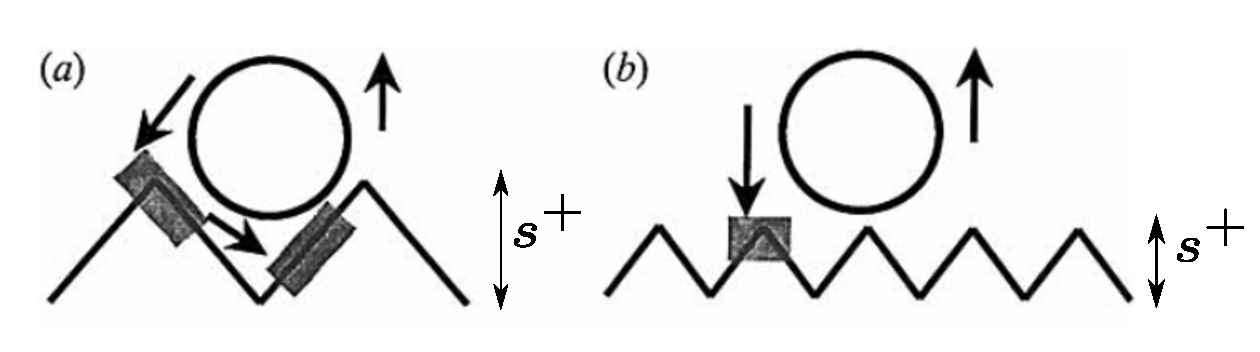
\includegraphics[width=0.7\linewidth]{chapter_1/riblets1}
	\caption{ ... \citet{choi1993direct} }
	\label{fig:riblets_schem}
\end{figure}

The slope of the curve \ref{fig:riblets_perf} can be predicted by linear stability theory or by means of empirical correlations as in \citet{garcia2011hydrodynamic}.

Computing the performance of such surfaces can be expensive since the most reliable quantitative theory for such problems are DNS simulations or experiments.
There is only one other theory, besides the already cited expensive ones, that use the concept of of \textit{protusion height} showed in \ref{fig:riblets1} to correlates the shape of the protusion to the drag reduction \citet{luchini1991resistance}.
The \textit{protusion height} is defined as the vertical distance between the riblet top ridge and point of zero velocity extrapolated from the constant velocity gradient outside above the protusions.
It seems that especially the difference of protusion heights computed from the streamwise $h_{ps}$ and cross-flow flow $h_{pc}$ correlates very well with the drag reduction, and the two quantities can be computed with a simple Stokes problem over the local geometry of the grooves.

Another very impressive characteristic is that the performance are robust in off-design, such as the yaw (misalignment between the flow and the riblets ridges) and tip erosion of the ridges \citet{garcia2011drag}.

But still besides some very specific application, such as  sailing competitions in which the hulls of the USA challengers in the America’s Cup 1987 and 2010 were fitted with riblets, the massive utilization of this technology is still in question.
Since the riblets size need to be very little, producing such surfaces in a larger area like the roof of a car or the wing of an airplane can be an issue for a routine use.

Riblets like surface has been observed in nature for many years, for example \citet{Martin2016riblets} found out that skimmer birds (Rynchops) have riblets like grooves in their beak, since they fly with it under the surface of the water to catch fishes.
But, as already introduced, the most clear example of such natural surfaces are shark skin.
In his review \citet{dean2010shark} present the status of the shape optimization that has been done on the riblets trying to mimic the typical sawthoot shape seen in shark skin, showing that improvements of such geometries over the classical ones has yet to be proven.
Shape optimization on riblets geometry has been studied also by \citet{bechert1997experiments} finding that the drag reduction can be improved very little just working on the geometry even though a few $\%$ can be gained.

There is in fact some controversial result in literature that state that surfaces with actual shark skin replica can indeed increase drag.
\citet{boomsma2016direct} for example perform some simulations on actual shark skin denticles using the immersed boundary method; he find that in some configuration 
the actual drag increase up to $40\%$, but even though the numbers are probably too large (it is know that the immersed boundary method can generate large errors in force computation especially in high Reynolds number flows), this can prove that the shark skin does not work with the same mechanism as riblets.

In fact \citet{bechert1997natural} had already tested such geometries in his experiments. 
He builds a synthetic surface made by artificial shark denticles posed on top of spings and he measure that even with the introduction of the surface elasticity the actual drag was increasing.
however the authors pinpoints that the actual shark flow regime is nothing at all as steady as the experiments that he performed, and he speculates that the excellent swimming performance of the shark came from the separation control that flexible denticles can increase in the periodic oscillating flow that the swimming generate.

Experiment using DPIV on a NACA covered with actual skin samples of "Isurus oxyrinchus" mako shark, has been performed by \citet{lang2014SharkControl}, confirming that the flexibility of sharks denticles perform as a passive flow control in order to avoid early separation.
In fact the experiments proves that for angles of attack larger than $15^{\circ}$ the flow reversal is almost completely avoided.
The same author introduce the importance in the different geometries of the denticles in different part of the body that obviously experience different flow condition,
\citet{motta2012Shark} perform a detailed collection of flexibility and scale measurement of different shark species that can be valuable for future studies.

Swimming experiment from \cite{Oeffner785}, who used a flat plate covered with real shark skin, also confirm the previous flow control mechanism and also make some conjectures about possible thrust enhancing controlled by the same movable scale that can move away the leading edge vortex.

Also \citet{itoh2006turbulent} shows that movable rugosities can outperform riblets, the authors in fact measure the drag reduction of a seal fur (that present fibrous movable surface) against a riblet surface in an experimental channel; its results are show in figure \ref{fig:seal}.

\begin{figure}[h]
\centering
\includegraphics[width=0.7\linewidth]{chapter_1/seal}
\caption{Image from \citet{itoh2006turbulent}.}
\label{fig:seal}
\end{figure}


Compliant surfaces can in fact move accordingly to the surface pressure gradients along the boundary layer and so respond to the pressure fluctuation over the surface itself.
This mechanism is already know to be beneficial to delay the transition to turbulence and many authors have presented theoretical and experimental evidence on the effectiveness of this solution \cite{carpenter1990status}, \cite{bushnell1977effect}.

So we have seen that to reduce turbulent skin-friction drag riblets and natural surfaces uses various mechanism such as: sublayer vortices interaction, compliance and separation control.
Such solution have proven to be effective in some cases but they are related mostly in reducing the viscous component of the total drag.
In the next section we will introduce another class of solution that try to act instead on the pressure component.


\subsection{Permeable surfaces}

More vertical extended porous surfaces instead try to act on the pressure drag contribution, that depends on the overall pressure distribution on the body.
Usually the pressure contribution is the most significant and even in highly streamlined body its around the $10\%$ of the total drag.



cita esperimenti tedeschi sul cilindro con il bordo d'uscita poroso, e lavoro sulla sfera di Giuseppe

Porous surface(mortazvi) per viscous pressure drag, (pressure redistribution)
\chapter{Volume Average Method}
\label{ch:vans}

\section{Introduction}


\section{Derivation of VANS equations for 3D incompressible fluids}
\subsection{Definition of the averaging filter}

In the figure \ref{fig:rev} is an illustration of our porous problem; in the same figure we show all the main definition that we need to introduce in order to develop our mathematical approach.


\begin{figure}[H]
	\centering
	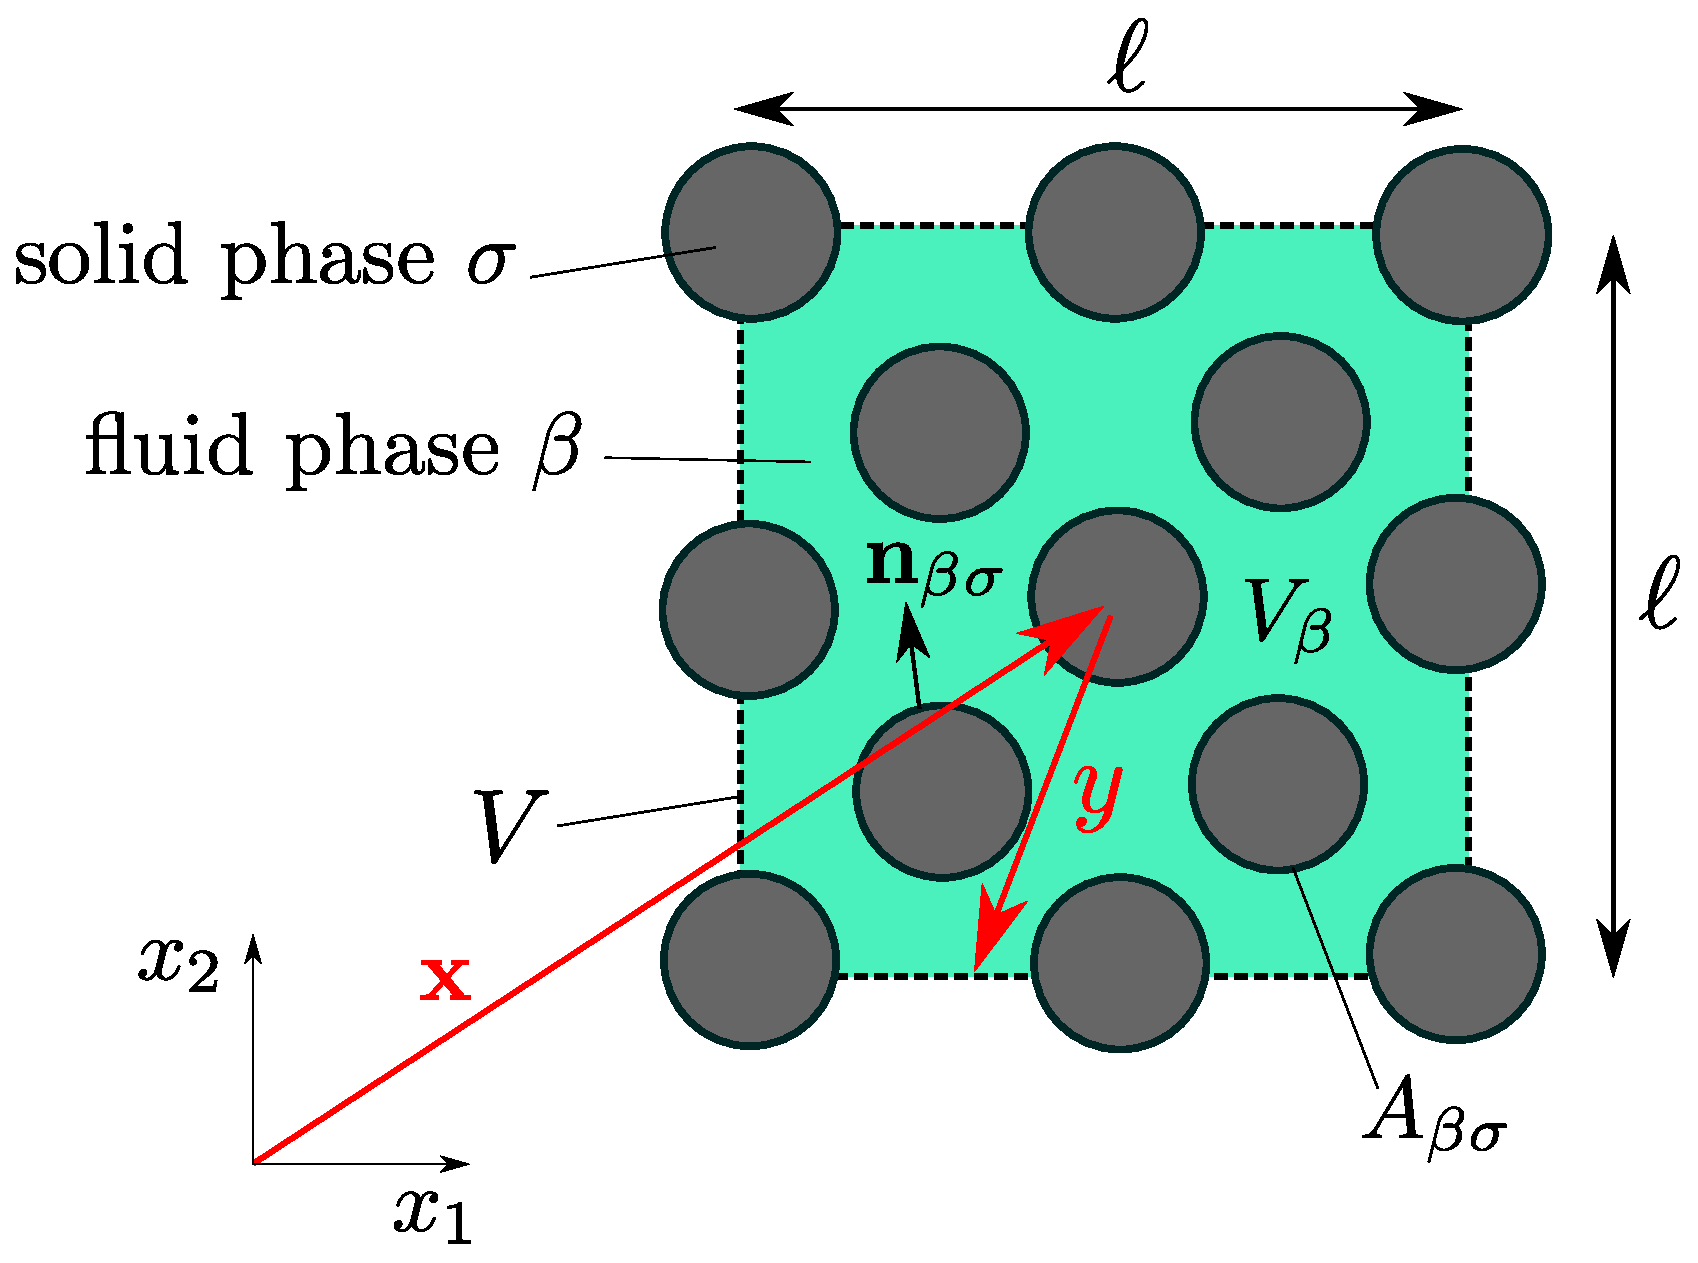
\includegraphics[width=0.8\linewidth]{chapter_4/figure/REV}
	\caption{Illustration of the REV concept.}
	\label{fig:rev}
\end{figure}


\begin{equation}
\meani{\psi_{\beta}}(\mathbf{X}, t) = \dfrac{1}{\volb} \int_{\volb} m(\mathbf{y}) \psi_{\beta}(\mathbf{x}-\mathbf{y}, t) d \volb.
\label{eq:avg_intrinsic}
\end{equation}


\begin{equation}
\meani{\psi_{\beta}}|_{\mathbf{x}} = \dfrac{1}{\volb} \int_{\volb(\mathbf{x})}  m(\mathbf{y}) \psi_{\beta}(\mathbf{x}-\mathbf{y}, t) d \volb.
\label{eq:avg_intrinsic_ext}
\end{equation}

\begin{equation}
\means{\psi_{\beta}} = \dfrac{1}{V} \int_{\volb} \psi_\beta (\mathbf{x}) d \volb.
\label{eq:avg_superficial}
\end{equation}


\begin{equation}
	\varepsilon = \dfrac{\volb}{V}
	\label{eq:porosity}
\end{equation}

\begin{equation}
	\means{\psi_{\beta}} =  \varepsilon \meani{\psi_{\beta}}
\end{equation}

\subsection{Theorems involving derivatives of spatial averaging}

\begin{theorem}[Averaging theorem Howes and Withaker, 1985]
\[	\means{\nabla \psi_{\beta}} = \nabla \means{\psi_{\beta}} + \dfrac{1}{V}\int_{A_{\beta \sigma}} \mathbf{n}_{\beta \sigma} \psi_{\beta} dA \]
\end{theorem}


\subsection{Length scale decomposition}

\begin{equation}
	\psi_{\beta} = \meani{\psi_{\beta}} + \tilde{\psi}_{\beta}
 \end{equation}

\subsection{Averaged continuity equations}


\begin{equation}
\nabla \cdot \vb = 0
\label{eq:cont}
\end{equation}

\subsection{Averaged momentum equations}


\begin{equation}
\dfrac{\partial \vb}{\partial t} + \vb \cdot \nabla \vb = -\frac{1}{\rho_{\beta}} \nabla \pb + \nub \nabla^2  \vb  + \mathbf{f}
\label{eq:mom}
\end{equation}



\subsubsection{Interface condition}

Penalization method \citet{angot1999penalization} used in\cite{bruneau2004passive} \cite{bruneau2008numerical} \cite{bruneau2010coupling}...


We think that using a boundary condition at the interface is not a superior approach nor physically neither mathematically.
Using penalization method the slip velocity at the interface can be computed as well as using a boundary condition, and either methods require a parameter to close the formulation, with the advantage using penalization method that the parameter is the spatial distribution of the porosity field that is trivial to compute known the geometry of the medium.

Also in case of very low Reynolds number the boundary condition can be a necessity since the Stokes equations, for the free fluid, and the Darcy one for the porous media are not mathematically compatible; but for $Re>10$ when the Brinkmann model for the porous media is applicable the two set of equations are of the same order and the continuity of pressure and velocity can be imposed directly.

Also there is evidence in literature through numerical and computational experiments \citet{ochoa2017fluid} that exist a transition zone with the size of the pore scale in which the velocity and pressure have a continuous variation.

\chapter{Drag-model sensitivity of Kelvin-Helmholtz waves in canopy flows}
\label{ch:stability}

\chapquote{While knowledge can create problems, it is not through ignorance that we can solve them.}{Asimov's New Guide to Science, 1984}{Isaac Asimov}

\citet{segura2017permeable} \Red{state that their results agree with yours ??}

Include this paper \citet{sharma2017stabilitycanopy}

cita \citet{ortiz2002spatial}


cita \citet{garcia2017analysis} nelle conclusioni dicendo che ha usato il nostro modello in caso turbolento ecc..

%%%%%%%%%%%%%%%%%%%%%%%%%%
\section{Introduction}
%%%%%%%%%%%%%%%%%%%%%%%%%%


\Red{modify the introduction to not repeat the same parts that you have presented in the intro}


Flows through submerged aquatic plants exhibit large scale vortices at the top of the vegetation,
advecting along the flow direction and causing a periodic waving of the plants, referred to as
monami (\citet{ackerman1993reduced}).  Vortices arise from the nonlinear amplification of a Kelvin-Helmholtz instability mode,
related to the presence of an inflection point in the base flow profile (\citet{asaeda2005morphological}); the profile itself is inflectional
because the fluid is slowed down by the drag exerted by the canopy, whose modeling has recently
been addressed (\citet{py2004mixing}, \citet{singh2016linear}, \citet{zampogna2016instability}). The correct prediction of the onset and characteristics of the Kelvin-Helmholtz
instability is important for assessing the effects of turbulence, in particular to
\begin{itemize}
	\item  understand how the vertical exchange of momentum occurs (\citet{ikeda1996three})
	\item clarify how the transport of $CO_2$ , dissolved nutrients or sediments takes place between the
	obstructed vegetation flow and the free overflow motion (\citet{gambi1990flume}, \citet{eckman1987role}, \citet{grizzle1996hydrodynamically}, \citet{finnigan2000turbulence}), and also
	\item assess the changes in the morphology of the vegetation in inland or coastal wetlands in
	response to continuous periodic forcing (\citet{asaeda2005morphological}, \citet{patil2010characteristics})
\end{itemize}

Because of the flexibility of the vegetation, some theoretical studies have focussed on the
modeling of the stems of the aquatic plants and their displacement in response to the forcing by the
water flow (\citet{py2004mixing}, \citet{patil2010characteristics}). However, Kelvin-Helmholtz vortices occur whether or not the plants bend and—to ascertain causes and effects to first order—it is acceptable to focus on the flow over and through a
submerged array of rigid, cylindrical pillars. This has been the basis of the approach by Ghisalberti
and Nepf (\citet{ghisalberti2002mixing}, \citet{ghisalberti2004limited}, \citet{ghisalberti2005mass}) who have conducted a series of careful experiments; their results have often been
used by fluid dynamicists to put forth and test theoretical hypotheses to predict the frequency and
wavelength of the large scale vortical motion, for a variety of conditions. The configuration studied
consists of a regular grid of rigid pillars, orthogonal to the surface, of identical height h; in some
of the theoretical models proposed to analyze the stability of this system, the Rayleigh equation is
used throughout the water channel, with or without a drag term in correspondence of the canopy (\citet{raupach1996coherent}, \citet{py2004mixing}, \citet{singh2016linear})
\citet{zampogna2016instability} have recently demonstrated that the addition of a drag term through the vegetation reduces the amplification factor of the Kelvin-Helmholtz instability throughout the whole
range of wavenumbers and increases mildly the wavelength of the fastest growing mode; further
unpublished work by the same authors shows that the addition of a mixing length turbulence model
in the stability equations has but a negligible influence on the leading instability mode. Questions
remain, however, on the accuracy of the drag model and on its sensitivity. A partial answer to these
questions is provided in \citet{zampogna2016instability}: there, a different model, applicable within the vegetated layer and
based on the equations ruling the behavior of a transversely isotropic porous medium, has been
developed and the stability results appear to better match experimental correlations. This conclusion
is, however, not consolidated yet, and further studies are needed to assess the influence of the model
of the drag force through the vegetation, both in setting up a particular (inflectional) mean flow and
on the onset and growth of Kelvin-Helmholtz waves.
The present work addresses the points above through an adjoint-based sensitivity analysis along
the lines of \citet{bottaro2003effect} the direct stability equations are written with account of viscosity, and
the adjoint equations are found and solved in the temporal framework. Results in the spatial setting
are discussed in Appendix B, where a digression is made on the computation of the group velocity
of the instability waves by the use of the adjoint fields. The sensitivity functions to both mild
modifications in the base shear layer and in the drag coefficient are computed and discussed. Finally,
a different sensitivity analysis is developed on the basis of the recent anisotropic model by \citet{zampogna2016instability} and the results qualitatively compared to those obtained with the more conventional
isotropic-drag-force model.



%%%%%%%%%%%%%%%%%%%%%%%%%%%%%%%%%%%%%%%%%%%%%%%%%%%%%%%%%%%%%%%%%%%%%%
\section{Model of the canopy flow}
%%%%%%%%%%%%%%%%%%%%%%%%%%%%%%%%%%%%%%%%%%%%%%%%%%%%%%%%%%%%%%%%%%%%%%
\label{sec:2ch3}

%%%%%%%%%%%%%%%%%%%%%%%%%%%%%%%%%%%%%%%%%%%%%%%%%%%%%%%%%%%%%%%%%%%%%%
\subsection{The mean flow}
%%%%%%%%%%%%%%%%%%%%%%%%%%%%%%%%%%%%%%%%%%%%%%%%%%%%%%%%%%%%%%%%%%%%%%

To obtain the mean flow on top of which small amplitude perturbations are superimposed, the
procedure outlined by \citet{ghisalberti2004limited} and recently closely followed by \citet{zampogna2016instability} is
used. For the sake of conciseness, the procedure which relies on several empirical correlations is
not repeated here, aside from a few brief comments. A mildly inclined water channel is considered, with a canopy formed by rigid cylindrical dowels of height $h$ equal to $13.8 \, cm$ and diameter
$d = 0.64 cm$. The frontal area of the vegetation per unit volume, i.e., the packing density of the
elements, is either $a = 0.04 cm^{-1}$ or  $0.08 cm^{-1}$ ; the free surface is positioned at a level $H = 46.7 cm$
from the bottom plate and the flow velocity at the free surface, $U_2$ , varies from $4.4$ to $13.7 cm/s$. The
Froude number, $F_r = \dfrac{U_2}{g H} $ is thus very low and water surface fluctuations can be ignored \citet{brevis2014experimental}. 
To a good approximation the mean flow can be taken as steady and parallel, with the streamwise
velocity varying from the value $U_1$ at the bottom wall (not accounting for the thin bottom boundary
layer) to the value $U_2$ at the top, near the free surface (\ref{fig:1}). The slope of the bottom surface is
very small; it is denoted as $S$ and, in the experiments by \citet{ghisalberti2004limited} varies from $1.8 \times 10^{-6}$ 
to $10^{-4}$; such a slope provides the driving force for the motion. The viscous term is small compared to
the turbulent diffusion term, so that the mean streamwise momentum equation can be approximated
by:
\begin{equation}
gS = \derp{\overline{u'v'}}{y} + \frac{1}{2} C_D(y) a {U(y)}^2 
\label{eq:1}
\end{equation}
with $g$ the acceleration of gravity and $C_D$ an isotropic drag function available from the experiments,
variable across the canopy and equal to zero when $y \geq h$.

\begin{figure}[h]
	\centering
	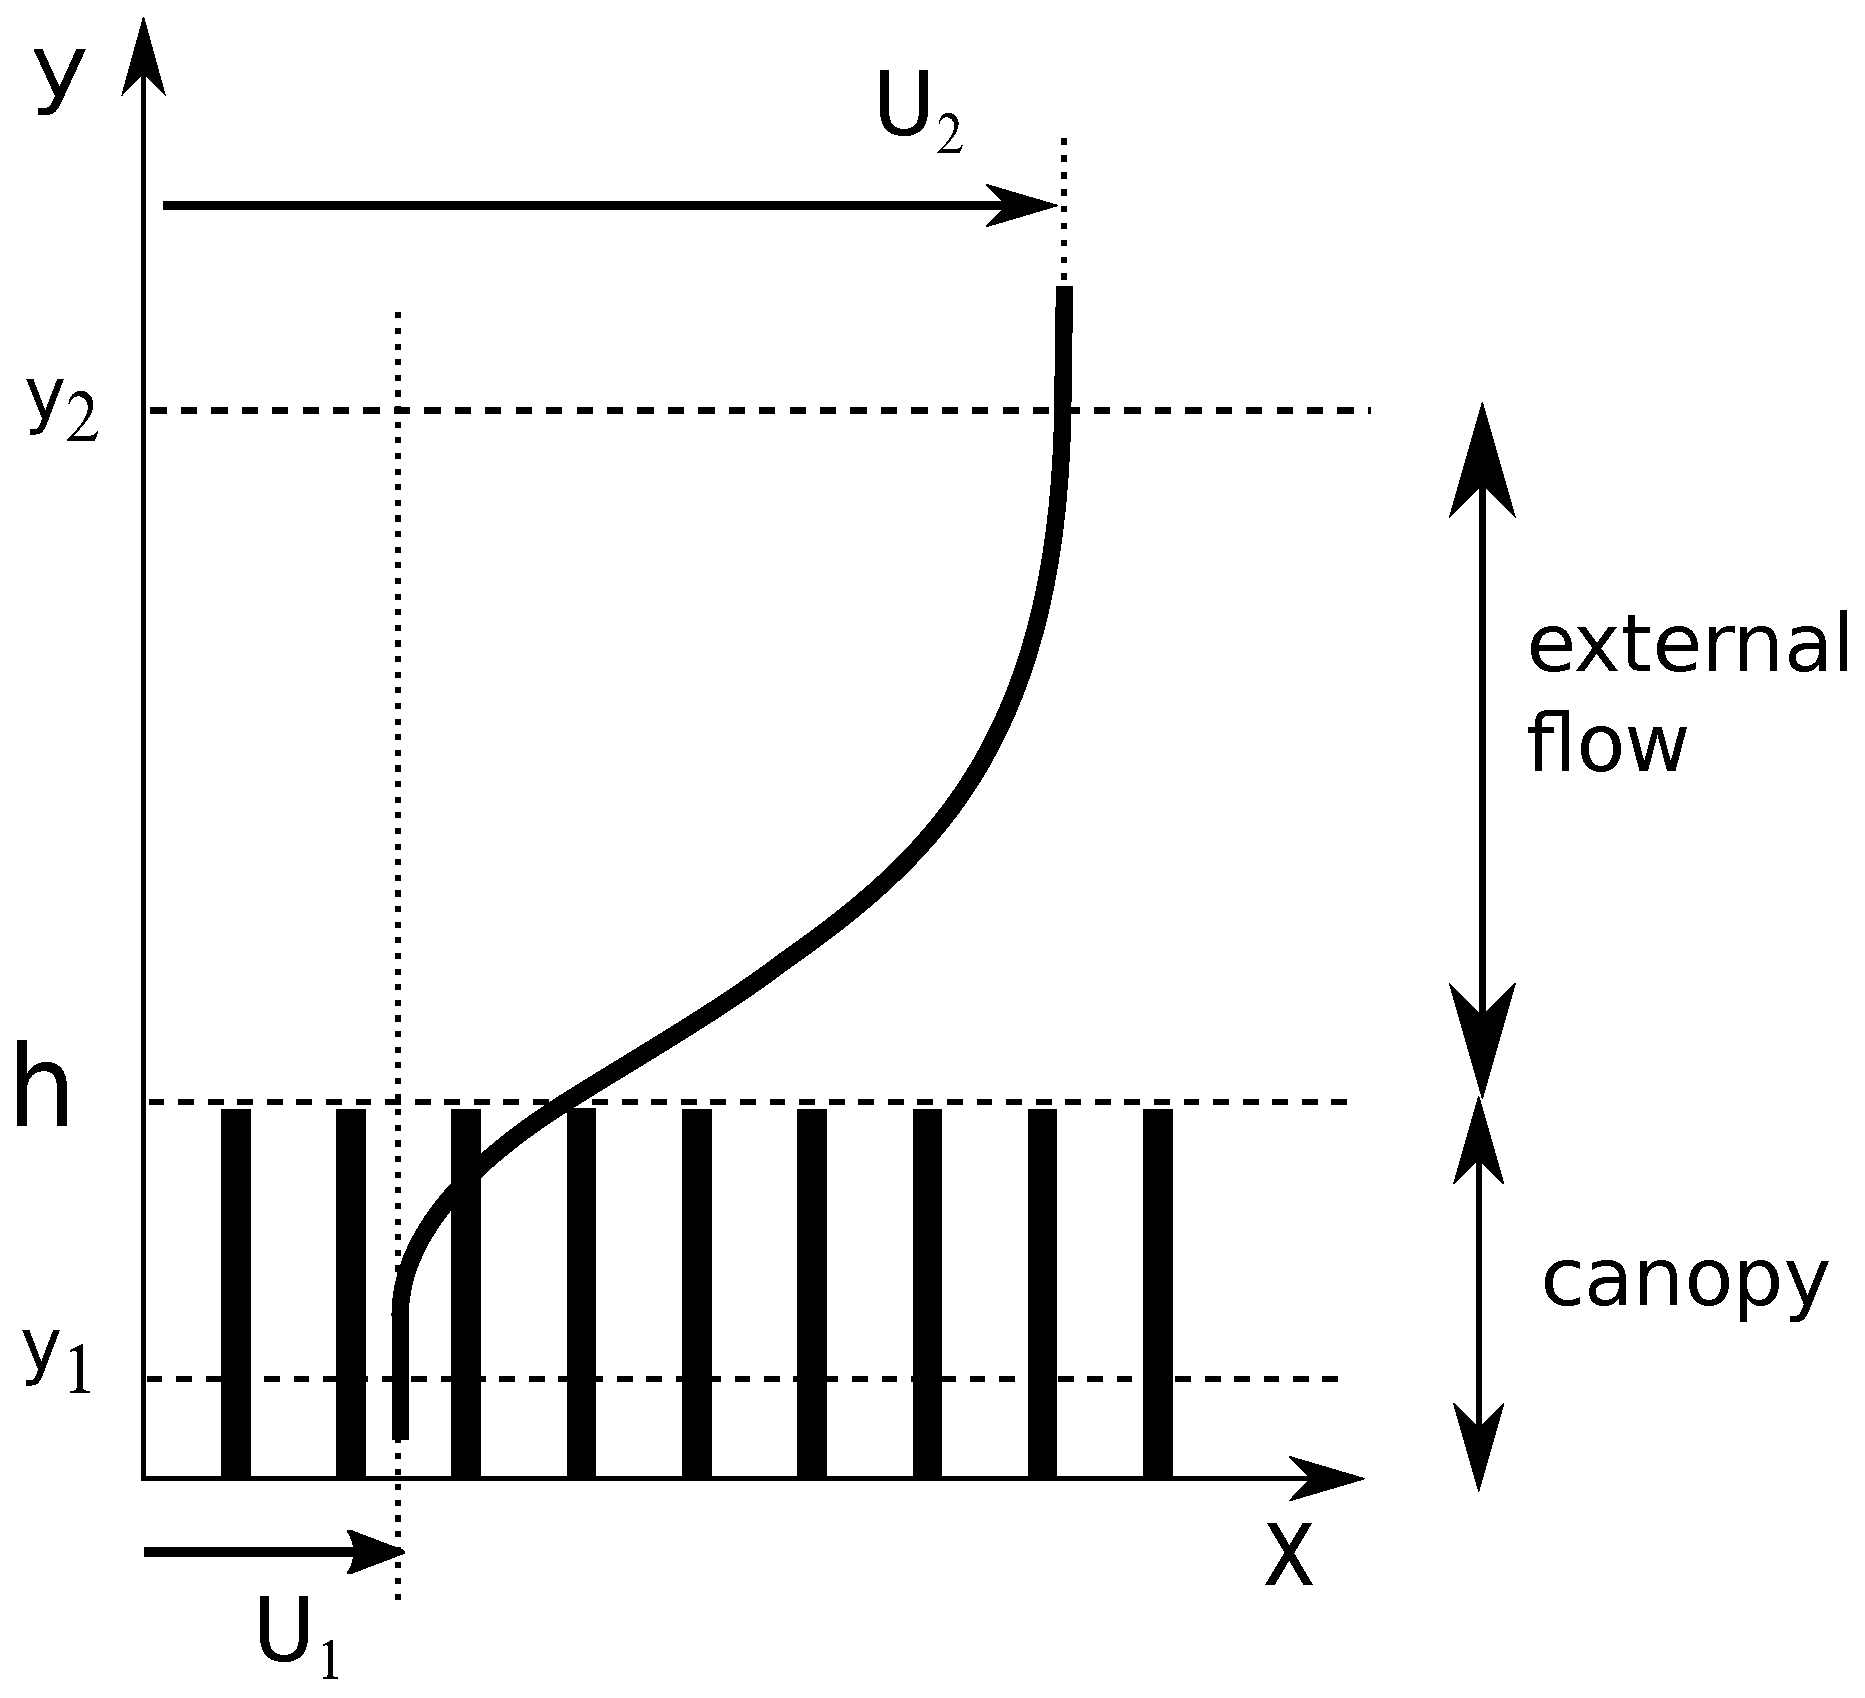
\includegraphics[width=0.5\linewidth]{chapter_3/figure/1}
	\caption{Configuration studied with main notations}
	\label{fig:1}
\end{figure}


\begin{figure}[h]
	\centering
	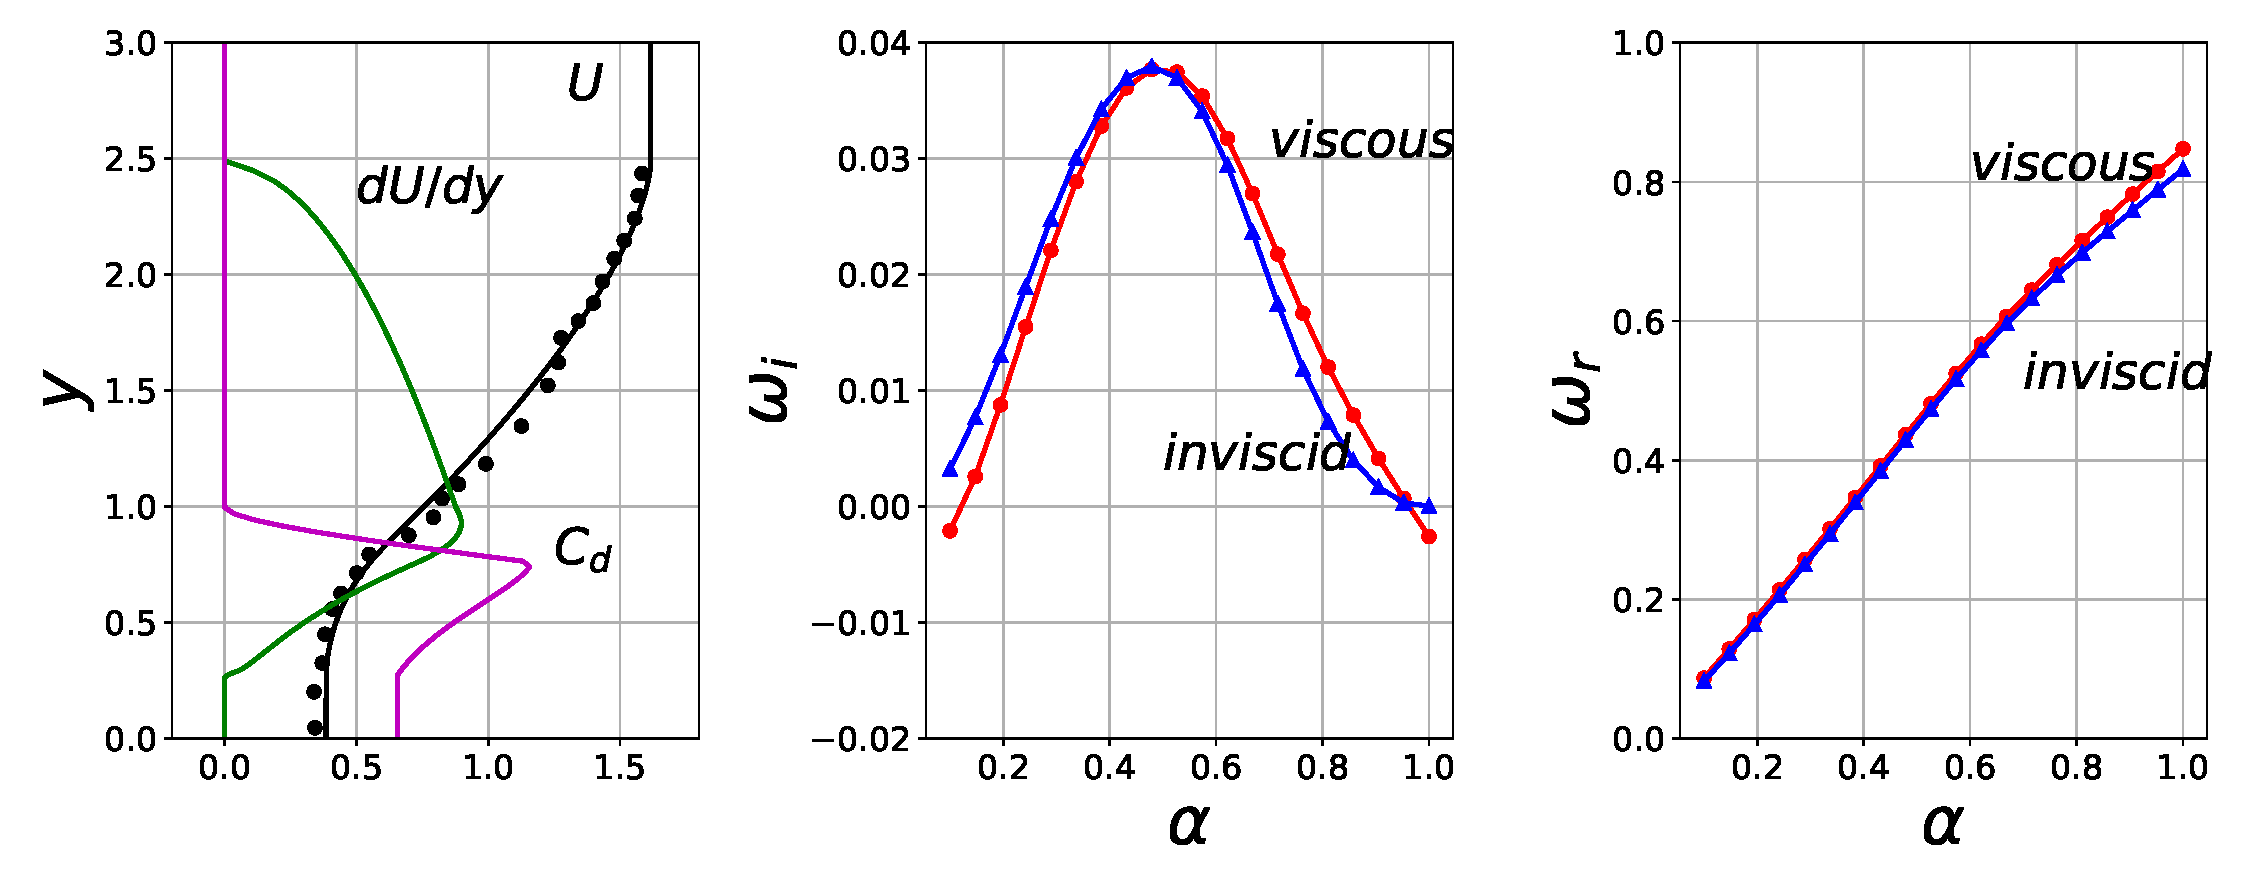
\includegraphics[width=1\linewidth]{chapter_3/figure/2}
	\caption{Left frame: mean flow U , together with experimental data points \citet{ghisalberti2004limited},  its first derivative, and drag coefficient
		distribution (case G). Center: viscous and inviscid growth rates, $\omega_i$ , as a function of the streamwise wavenumber $\alpha$. Right:
		corresponding frequencies, $\omega_r$}
	\label{fig:2}
\end{figure}



The Reynolds stress $\overline{u'v'}$ is modelled with
the Boussinesq assumption, introducing a turbulent viscosity which depends on a mixing length and
on the gradient of the mean velocity U. Referring to \citet{ghisalberti2004limited} for details of the empirical
correlations used to close the equations and the solution method, we limit ourselves here to stating
that the results obtained for the mean flow are very close to those reported in \citet{zampogna2016instability} (cf.
their Figure 3) and closely match experimental points for the cases G, H, I, and J considered (we use
the same terminology of\citet{ghisalberti2002mixing} \citet{ghisalberti2004limited} \citet{ghisalberti2005mass} to indicate the different flow configurations). An
example of mean flow is reported in \ref{fig:2} (left frame). There, one can observe the computed flow
(against discrete measurement points), its first derivative, and the drag coefficient distribution for one
representative case (experiment G), used below also to discuss stability and sensitivity results.
Other procedures have been employed in the past to calculate the mean flow, with satisfactory
results. For example,\citet{singh2016linear} have considered a constant value of $C_d$ through the canopy, while
\citet{zampogna2016instability} have coupled, at a fictitious interface, the fluid equations outside the canopy
to Darcy’s law within the vegetation. Thus, for the purposes of the present paper, the mean flow is
assumed as given; it could be, for example, simply a fit through experimental data. Nonetheless, in
Appendix A we provide some considerations on how $C_d$ affects the mean flow in the model used here.


%%%%%%%%%%%%%%%%%%%%%%%%%%%%%%%%%%%%%%%%%%%%%%%%%%%%%%%%%%%%%%%%%%%%%%
\subsection{Stability and sensitivity equations}
%%%%%%%%%%%%%%%%%%%%%%%%%%%%%%%%%%%%%%%%%%%%%%%%%%%%%%%%%%%%%%%%%%%%%%
\label{sec2b}
A temporal linear stability analysis is carried out, with the generic perturbation $q'(x, y,t)$ of the
form

\begin{equation}
q'(x,y,z,t)=\tilde q(y){\rm e}^{i(\alpha \  x -\omega \ t)}
\label{eq:q}
\end{equation}

with $\alpha$ the real streamwise wavenumber and $\omega$ a complex number whose real part, $\omega_r$ , is the fre-
quency of the mode and the imaginary part, $\omega_i$ , is the growth rate. The dimensionless linear stability
equations in primitive variables read

\begin{equation}
\begin{split}
& i\alpha u + D v =0,  \qquad D=d/dy \vspace{0.3cm}\\
& \left [ i (\alpha U -\omega)   - \frac{D^2-\alpha^2}{Re}+ a C_d U \right] u + U' v + i \alpha p  = 0,  \qquad U'=\dfrac{d U}{dy} \vspace{0.3cm} \\
& \left[ i (\alpha U -\omega)   - \frac{D^2-\alpha^2}{Re} \right ] v + D p   = 0
\label{eq:uvp}
\end{split}
\end{equation}

with the perturbation velocity components which vanish when $y=0$ and $y_{\infty}$. The upper boundary
of the computational domain is taken far enough away from the lower boundary to ensure that the
results do not vary upon modifications of $y_{\infty}$ . All the terms in the equations are dimensionless; the
mean speed through the shear layer, $U_m = \dfrac{U_1 +U_2}{2}$ , is used to scale the disturbance velocity components, pressure is scaled with
$\rho {U_m}^2$ , distances with $h$, and time with $h/U_m$ . The Reynolds number
in the equations above is thus defined as $Re = \rho U_m/ \mu h$ , with $\rho$ and $\mu$ the fluid’s density and dynamic
viscosity, respectively. The computations are performed both at the $Re$ values of the experiments
and in the inviscid limit (${Re}^{-1}  \rightarrow 0$ ), for comparison purposes. In the latter case, the boundary
conditions are simply $v = 0$ at $y = 0$ and $y_{\infty}$ .
System \ref{eq:uvp} above and its boundary conditions are, in the following, also written in short
notation as $\mathscr{L} q = 0$. The eigenvalues of the system are those complex values of $\omega$ which yield
non-trivial solutions for $u$, $v$, and $p$. Two numerical collocation codes are written, and success-
fully compared; one is based on the equations in primitive variables form, the second solves an
Orr-Sommerfeld-like equation (with the addition of the drag term) along the lines of \citet{singh2016linear}.
In both cases, a spectral scheme based on N Chebyshev polynomials is used (N is typically equal
to 300 to ensure grid-converged results), with an algebraic mapping between the physical and the
spectral domains (\citet{hussaini1987spectral} ).
Viscous and inviscid stability results for case G are shown in \ref{fig:2} (center and right frames);
differences are small, in consideration of the fact that the Reynolds number of the viscous case
is relatively large ($Re = 3450$). The viscous wavenumber of largest amplification is found for
$\alpha = 0.4790$; the waves are weakly dispersive, particularly at low wavenumbers (an original inter-
pretation of phase and group velocities is proposed in Appendix B). The wavelength of largest
growth is smaller than that found by \citet{zampogna2016instability} which was $0.73$; this is related to the slightly
different base flow in the two cases (in the present contribution a smoothing has been applied to the
$U$ velocity distribution to render $dU/dy$ continuous across $y$) and highlights the sensitivity of this
stability problem to base flow variations.
Following \citet{bottaro2003effect} it is assumed that small variations in base flow and drag coefficient
entail infinitesimal variations in the system’s eigenvalues and eigenfunctions. We stress here the fact
that $C_d$ is identically equal to zero outside of the canopy, and this implies that there are no possible
variations in $C_d$ for $y \geq 1$. The sensitivity functions to variations in $U$ and $C_d$ are obtained by using
the properties of the adjoint system which is defined from the Lagrange identity

\begin{equation}
0 = \delta \langle q^{\dagger}, \mathscr{L} q \rangle = 
\langle q^{\dagger}, \mathscr{L} \delta q \rangle +
\langle q^{\dagger}, \derp{\mathscr{L}}{U}  q \delta U\rangle +
\langle q^{\dagger}, \derp{\mathscr{L}}{C_d}  q \delta C_d\rangle +
\langle q^{\dagger}, \derp{\mathscr{L}}{\omega}  q \rangle \delta \omega
\label{eq:lagid}
\end{equation}

\begin{figure}[H]
	\centering
	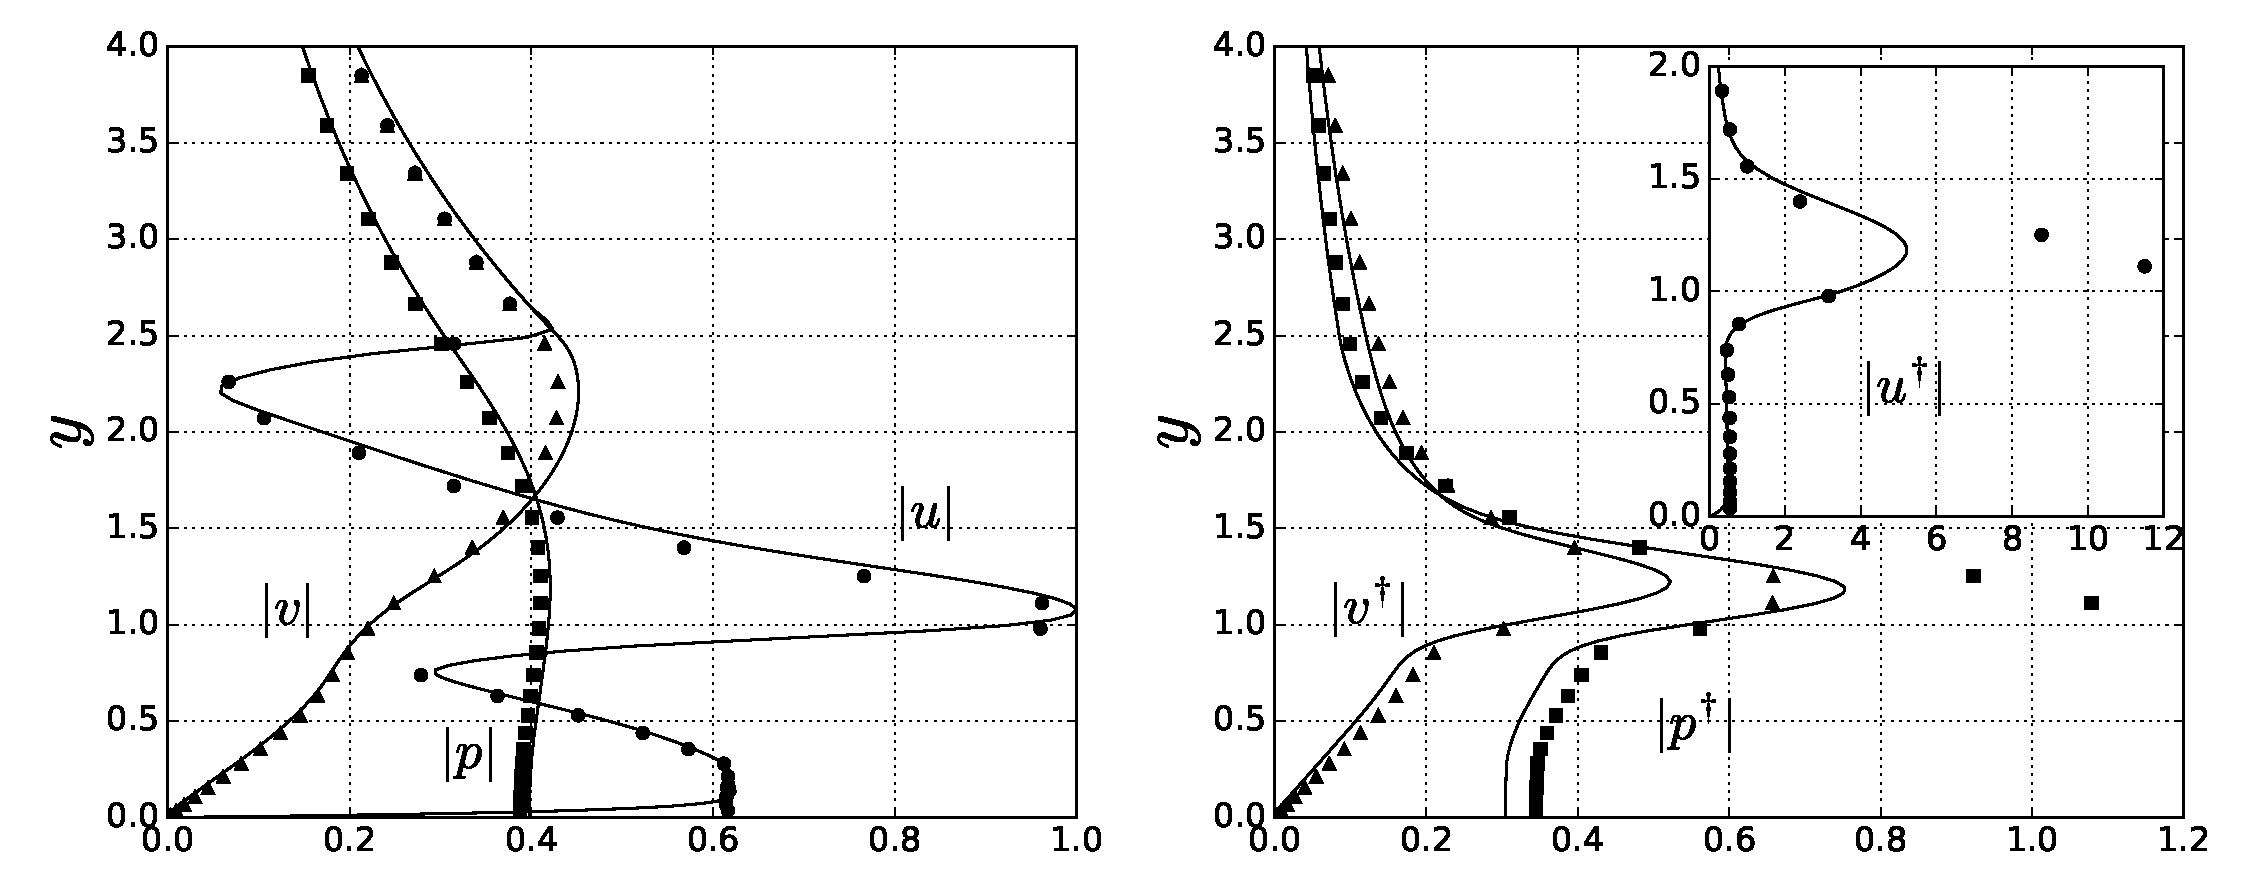
\includegraphics[width=1\linewidth]{chapter_3/figure/3}
	\caption{Moduli of direct (left frame) and adjoint (right frame) eigenfunctions for the viscous (continuous lines, $Re = 3450$)
		and the inviscid (symbols) case, in correspondence to the wavenumber of largest amplification.}
	\label{fig:3}
\end{figure}

and considering the effect of independent variations of $U$ and $C_d$ onto $q$ and $\omega$. It is found that

\begin{equation}
\delta \omega =\delta \omega_r + i \delta \omega_i= \int_0^{y_{\infty}}  G_U(y) \delta U(y) dy + \int_0^{1}  G_{C_D}(y) \delta C_D(y) dy
\label{eq:s_omega}
\end{equation}

with

\begin{equation}
\begin{split}
&G_{U} =  \alpha \left[ \overline{v^{\dagger}} v + \overline{u^{\dagger}} u  \right] +i   (\overline{u^{\dagger}}   v)' -i a C_d \overline{u^{\dagger}}  u \vspace{0.3cm}\\
&G_{C_D} =  - i \alpha  U  \overline{u^{\dagger}} u
\label{eq:GCD}
\end{split}
\end{equation}

the required sensitivity functions; the real parts of $G_U$ and $G_{C_d}$ express sensitivities to variations in
the frequency of the mode while the imaginary parts are sensitivities to variations in the growth rate.
Direct and adjoint eigenfunctions are normalized so that $N_{\omega} = 1$, with

\begin{equation}
N_{\omega} = \int_0^{y_{\infty}} \left[ \overline{ v^{\dagger}} v  +  \overline{ u^{\dagger}} u \right] dy
\label{eq:norm}
\end{equation}

An example of direct and adjoint eigenfunctions is provided in \ref{fig:3}, both in the viscous case
($Re = 3450$) and in the inviscid limit, for $\alpha = 0.4790$. It is interesting to observe that while the
direct eigenfunctions are almost overlapped, the same is not the case for the adjoint eigenfunctions,
with the inviscid mode (drawn with symbols) which has a larger amplitude than the viscous one.
The shapes of the direct eigenfunctions are very close to those reported in \citet{zampogna2016instability}. The adjoint modes
reveal that the flow is most sensitive to streamwise forcing, particularly when it occurs slightly
above the edge of the canopy. Source terms in the mass conservation and in the vertical momentum
equations are much less effective.


%%%%%%%%%%%%%%%%%%%%%%%%%%%%%%%%%%%%%%%%%%%%%%%%%%%%%%%%%%%%%%%%%%%%%%
\section{Sensitivity results for the isotropic drag model}
%%%%%%%%%%%%%%%%%%%%%%%%%%%%%%%%%%%%%%%%%%%%%%%%%%%%%%%%%%%%%%%%%%%%%%
\label{sec:3}

Some representative sensitivity functions are plotted in \ref{fig:4}; viscous and inviscid results
concur in showing that the largest sensitivities to variations of U are found right above the vegeta-
tion’s edge, where there are peaks in the adjoint eigenfunctions and where $d^2 U/d y^2$ vanishes. The
$U$-sensitivities are negligible within the vegetated layer and for values of $y$ larger than twice the
canopy’s height. The $C_d$-sensitivities are non-negligible only in close proximity of the interface.
It is interesting to observe that real and imaginary parts of the $U$-sensitivity functions are
shifted in y with respect to one another; this means that, for example, a localized perturbation at
a given $y$ position (above the canopy) might have a strong repercussion on the growth rate but not
on the frequency of the most unstable Kelvin-Helmholtz mode, or vice versa. Comparing left and
right frames of the figure, it is seen that inviscid $G_U$ sensitivity functions display sharper peaks and
steeper gradients, and yield larger variations in $\omega$ than their viscous counterparts in the proximity of
the $U$ inflection point, a clear consequence of the inviscid mechanism ruling the instability. In both
the viscous and the inviscid models, the sensitivity to base flow variations is typically one order of
magnitude larger than the sensitivity to changes in the drag coefficient.

\begin{figure}[H]
	\centering
	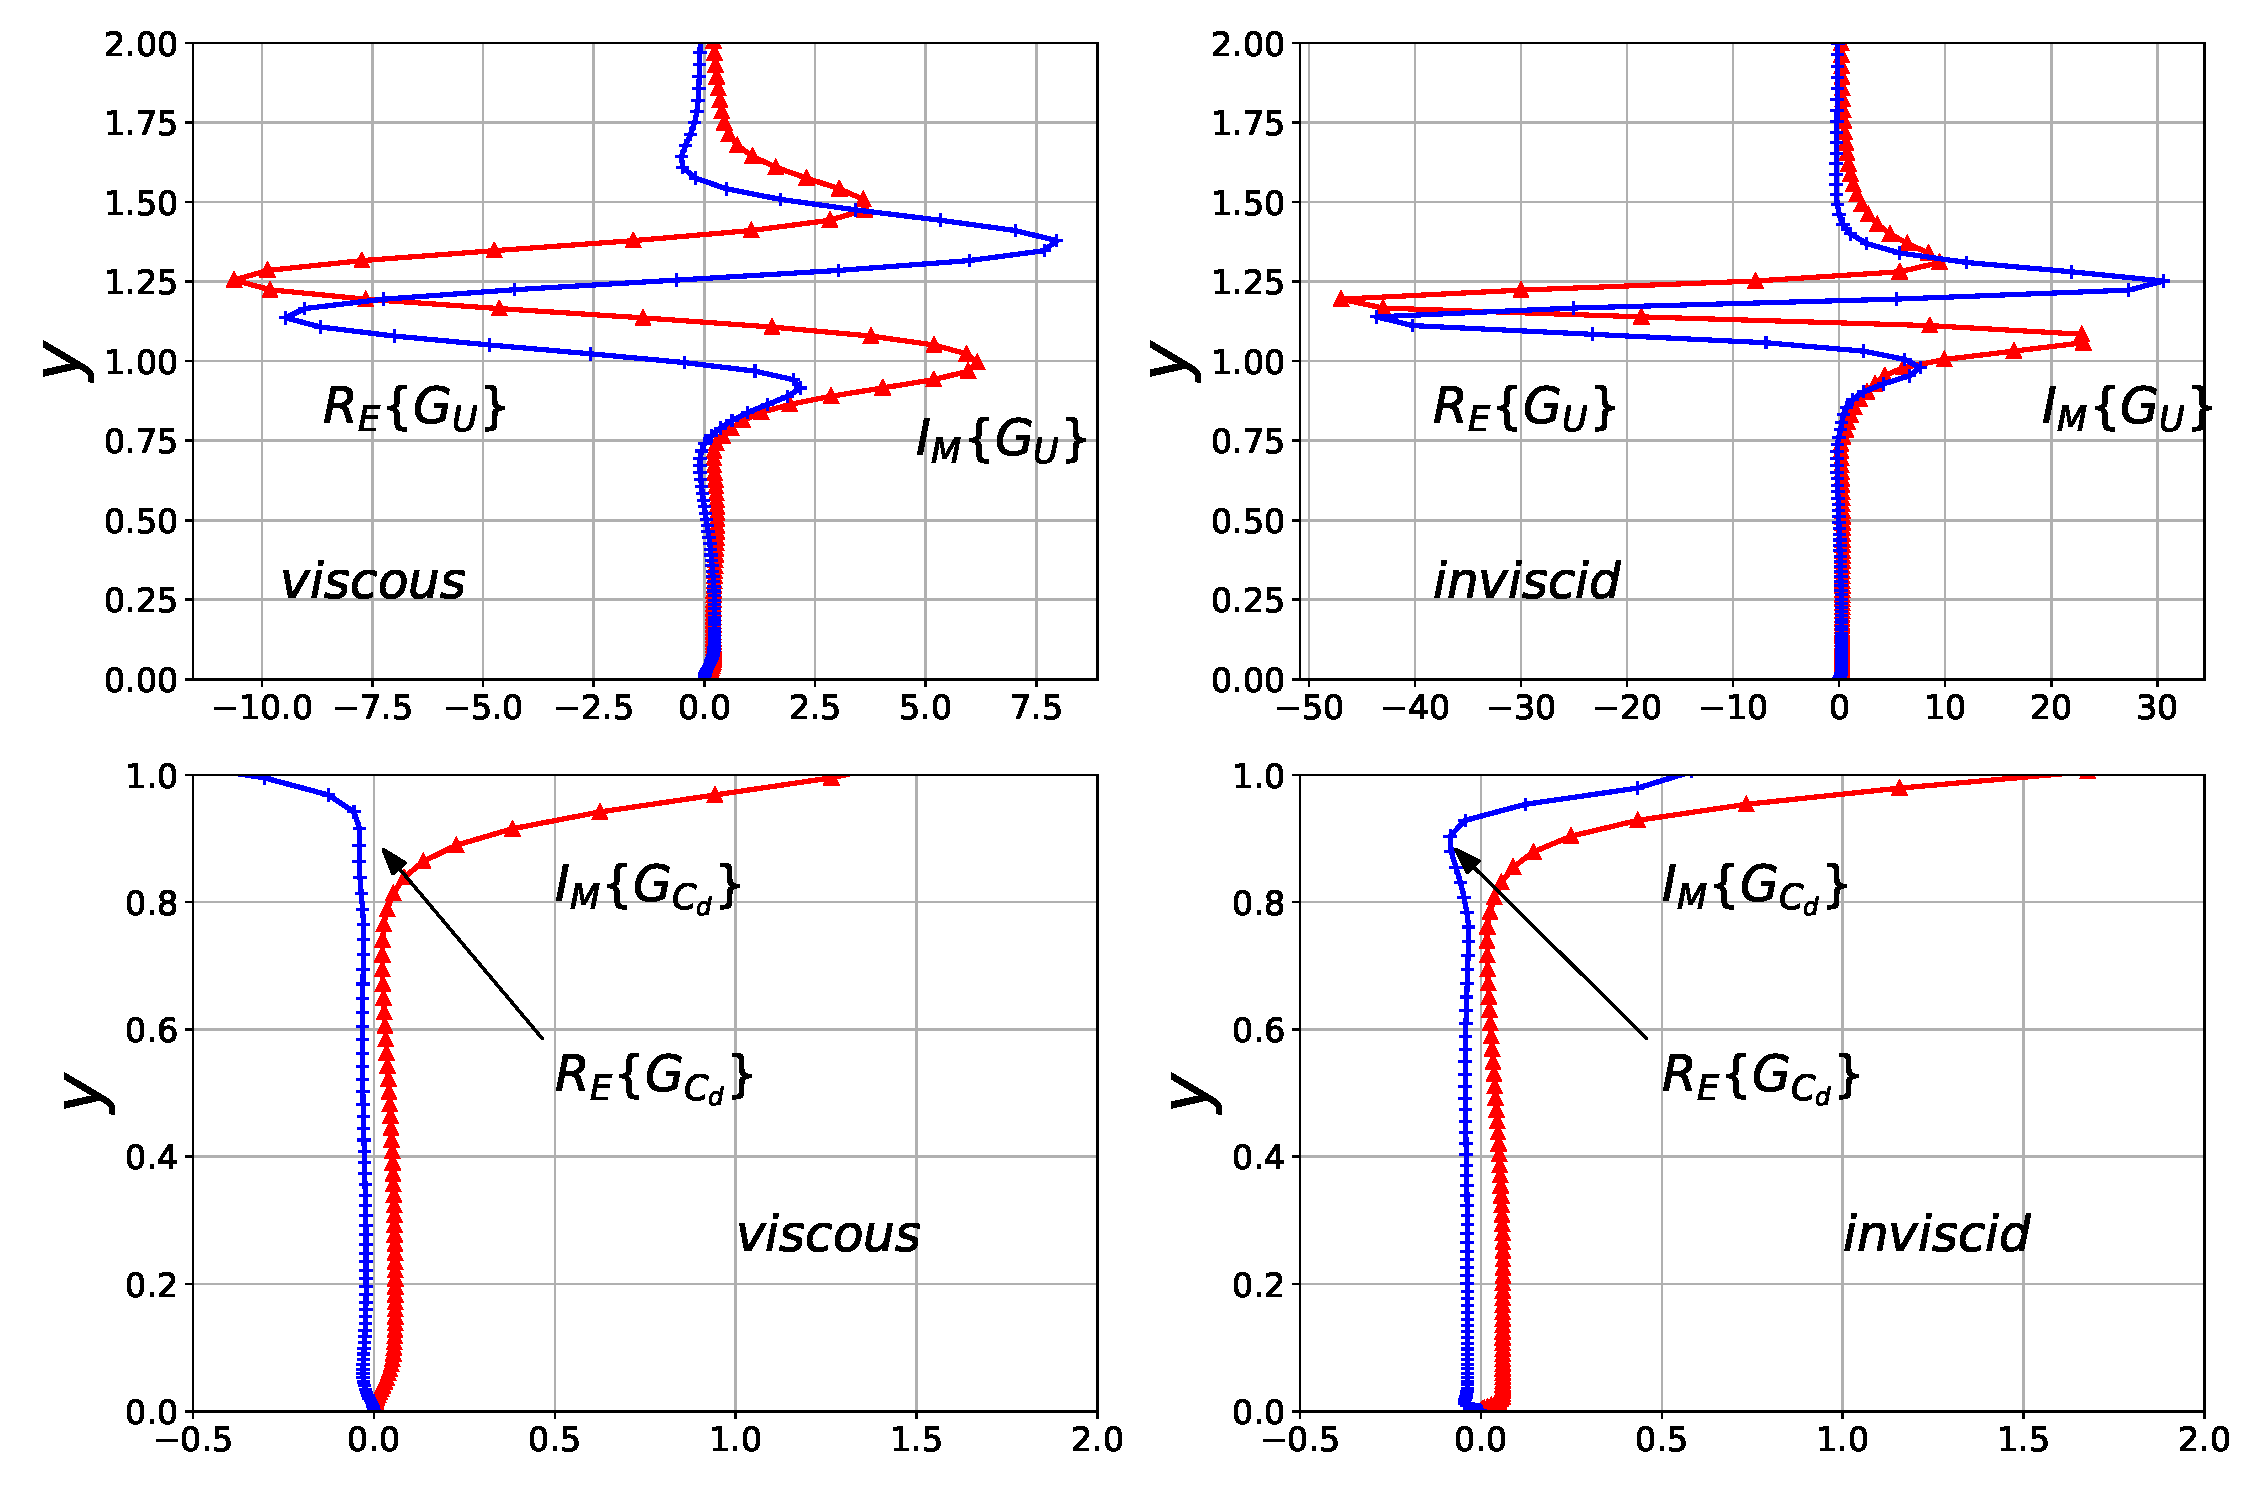
\includegraphics[width=1\linewidth]{chapter_3/figure/4}
	\caption{Real and imaginary parts of the sensitivities to mean flow variations (top) and to variations in the drag distribution
		function (bottom), for the parameters of \ref{fig:3}}
	\label{fig:4}
\end{figure}

The infinite norm of the sensitivities for the four cases studied (G, H, I, and J) is reported in
\ref{fig:5}; the main result found is that ${|G_U|}_{\infty}$ grows monotonically with $\alpha$ (and more so in the inviscid
case) whereas ${|G_{C_d}|}_{\infty}$ does not. It is consistently found that ${|G_U|}_{\infty}$ of case H is larger than that of
case I, which exceeds the corresponding value of case J, in turn larger than${|G_U|}_{\infty}$ of case G. This is
not unexpected in view of the values of the mean shear $\dfrac{U_2 - U_1}{H}$  which are, going from H to G, equal

\begin{figure}[H]
	\centering
	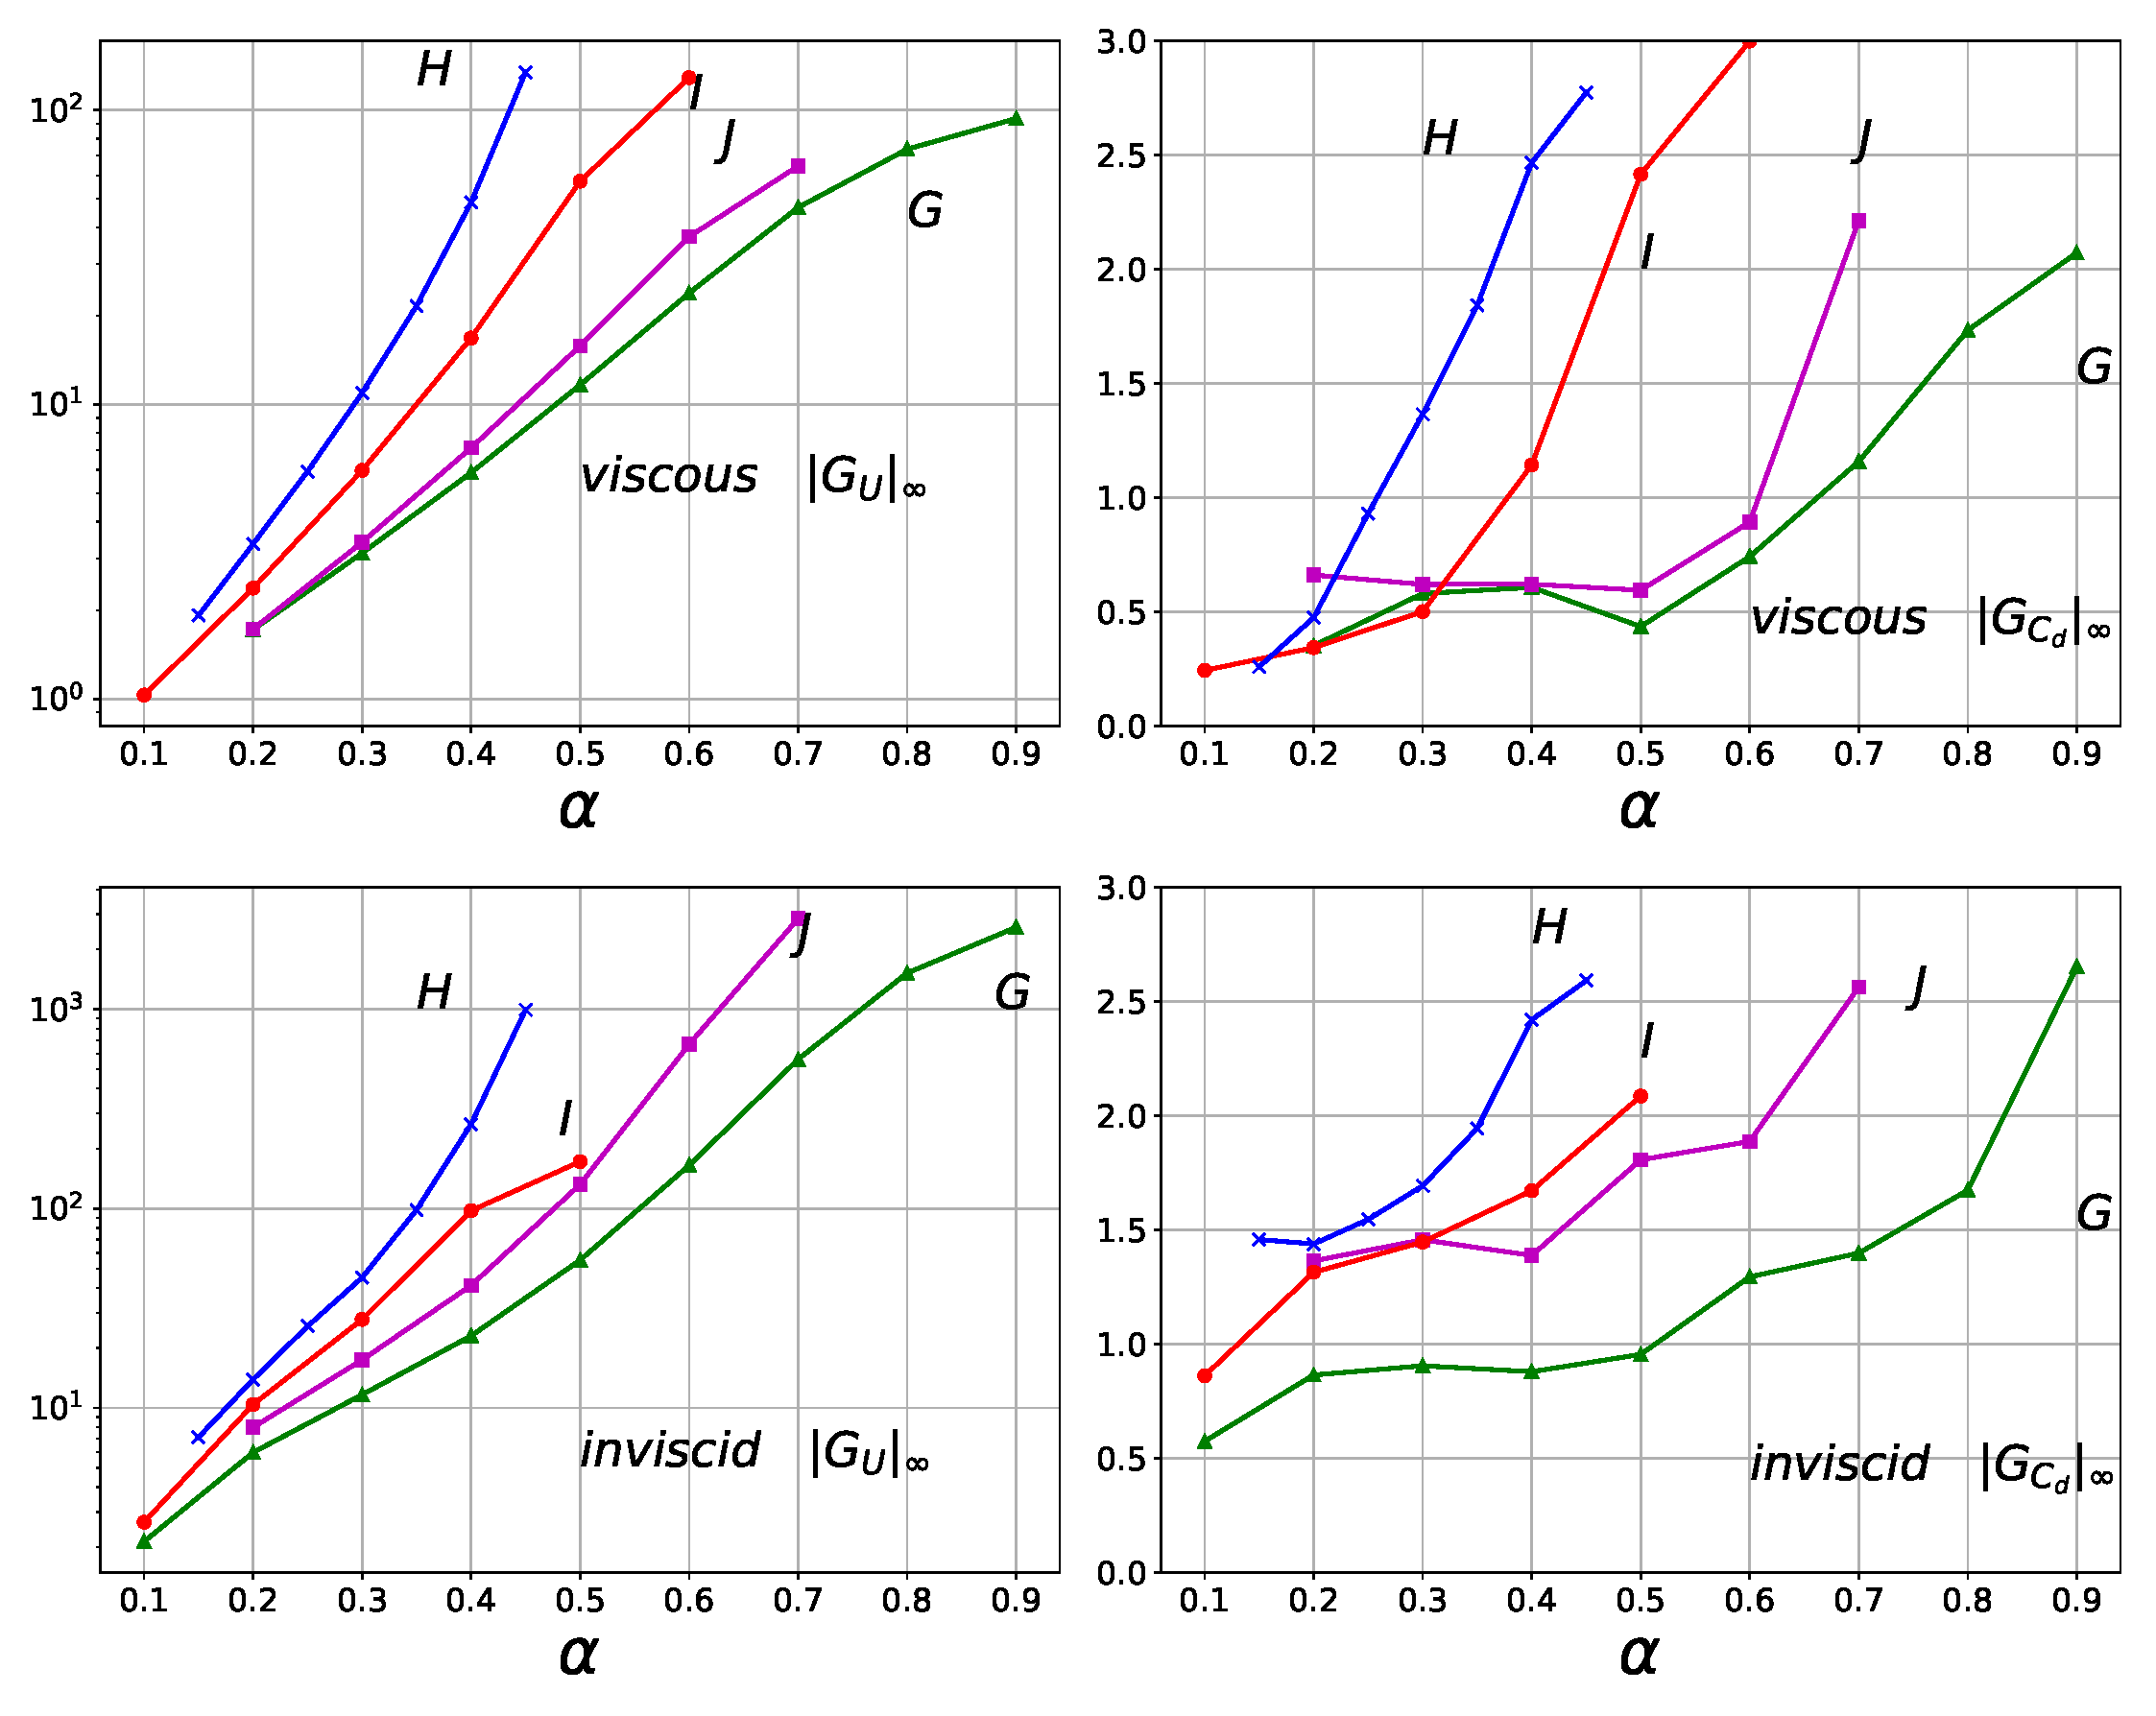
\includegraphics[width=1\linewidth]{chapter_3/figure/5}
	\caption{Infinite norms of the sensitivity functions for varying $\alpha$}
	\label{fig:5}
\end{figure}

to $0.236$, $0.158$, $0.084$, and $0.071 s^{-1}$ , respectively. The sensitivity of the eigenvalue $\omega$ to variations
in the mean flow is generally stronger than the corresponding sensitivity to variations in the drag
coefficient (aside for the long wave limit, where they are comparable). This might be interpreted
positively, considering that the use of a scalar coefficient $C_d$ to represent the drag within the canopy
is but a crude approximation. An alternative model to represent the flow throughout a network of
rigid, cylindrical dowels has recently been proposed by \citet{zampogna2016instability} The sensitivity results for
such a new model are discussed next.


%%%%%%%%%%%%%%%%%%%%%%%%%%%%%%%%%%%%%%%%%%%%%%%%%%%%%%%%%%%%%%%%%%%%%%
\section{An alternative sensitivity model: accounting for the canopy anisotropicity}
%%%%%%%%%%%%%%%%%%%%%%%%%%%%%%%%%%%%%%%%%%%%%%%%%%%%%%%%%%%%%%%%%%%%%%
\label{sec:4}

The stability problem in this section is based on the coupling between two regions, one outer
region dominated by inertia and ruled by the inviscid equations and an inner one dominated by
viscosity and ruled by Darcy’s law, with account of the canopy geometry through a tensorial
permeability, as described by \citet{zampogna2016instability} Normalizing the disturbance equation which couples
pressure and velocity in the inner region with the same scales as previously, we obtain

\begin{equation}
{u_i}' = -Re \dfrac{d}{ah^2} \mathcal{K}_{ij} \derp{p'}{{}x_j}',  \qquad (x_1, x_2) = (x,y)
\label{eq:darcy}
\end{equation}


with $\mathcal{K}_{ij}$ the dimensionless permeability. The effective interface between the inertial region and the
slow, viscosity-dominated region does not coincide with the edge of the canopy; in fact, the rapid
outer flow penetrates through the upper part of the vegetation and an effective matching between
outer and inner flows must be enforced some distance $\delta$ below the canopy’s edge \citet{le2006interfacial}.  This distance,
a penetration depth, has been successfully computed by \citet{zampogna2016fluid} for a few cases
and is found to increase with the Reynolds number of the flow; for experiment G discussed below it
is$ \delta = 0.40$ \citet{zampognaprivate}. On account of the results shown in \ref{fig:4}, with the sensitivities which are negligible
for $y \approx 0.60$, we expect that the exact position of the effective interface will not affect the results
significantly.
Using the fact that the velocity within the orthotropic porous medium is divergence free, the
interface condition to be applied at $y_{itf} = 1 - \delta$ is found to be \ref{eq:darcybc}

\begin{equation}
v|_{itf} + B(\alpha) p|_{itf} = 0
\label{eq:darcybc}
\end{equation}

with

$$
B(\alpha) = Re \dfrac{d}{ah^2} \sqrt{\mathcal{K}_{11}\mathcal{K}_{22}} \alpha \tanh (\theta), \qquad \theta = \alpha \sqrt{\dfrac{\mathcal{K}_{11}}{\mathcal{K}_{22}}}  y_{itf}
$$

The second boundary condition that the Rayleigh stability equation must satisfy at $y_{\infty}$ is sim-
ply $v = 0$. Thus, we solve only for the inviscid flow in the outer region, and the permeability
of the inner domain enters the equations only through the interface condition \ref{eq:darcybc}. $\mathcal{K}_{ij}$ is a two-
by-two diagonal tensor; $\mathcal{K}_{11}$ is the component of the dimensionless permeability along $x$ and
$\mathcal{K}_{22}$ is the $y$ component. For case G considered here, the packing density of the elements is
$a = 0.04 cm^{-1}$ ; it is also found that $\mathcal{K}_{11}= 0.0512$ and $\mathcal{K}_{22} = 0.0575$ \citet{zampognaprivate},  so that the function $B(\alpha)$
reads $B = 15.727 \alpha \tanh (0.566 \alpha)$.


%%%%%%%%%%%%%%%%%%%%%%%%%%%%%%%%%%%%%%%%%%%%%%%%%%%%%%%%%%%%%%%%%%%%%%
\subsection{The sensitivity equations}
%%%%%%%%%%%%%%%%%%%%%%%%%%%%%%%%%%%%%%%%%%%%%%%%%%%%%%%%%%%%%%%%%%%%%%

The adjoint equations in this case are the same as system \ref{eq:uvp}, without the terms containing $1/Re$
and $C_d$ , and the boundary conditions are

\begin{equation}
v^{\dagger}|_{itf} - B(\alpha) p^{\dagger}|_{itf} = 0, \qquad v^{\dagger}|_{y_{\infty}} = 0
\label{eq:darcybc_adjoint}
\end{equation}

The variation in the complex frequency is related to variations in the mean flow and in the perme-
ability components through the equation

$$
\delta \omega = \int_{y_{itf}}^{y_{\infty}}  G_U(y) \delta U(y) dy + G_{\mathcal{K}_{11}} \delta \mathcal{K}_{11} + G_{\mathcal{K}_{22}} \delta \mathcal{K}_{22}
$$

\begin{figure}[H]
	\centering
	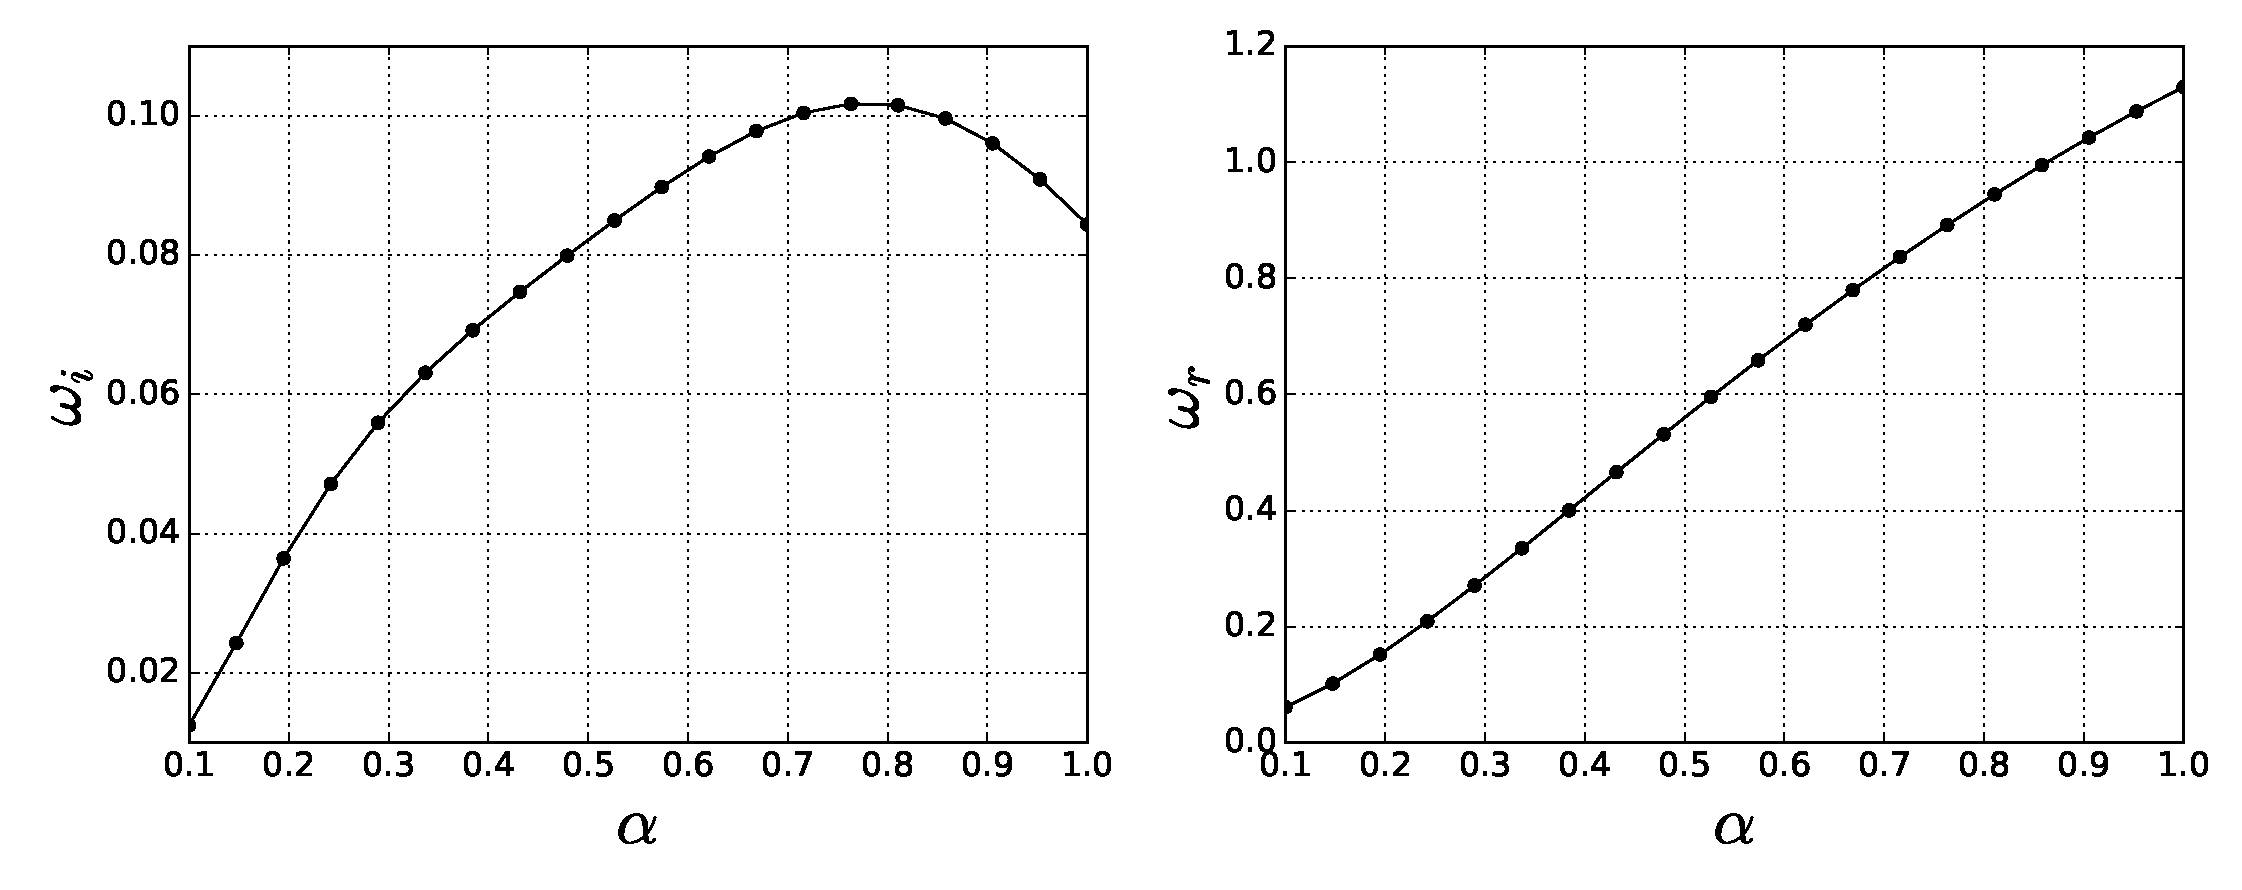
\includegraphics[width=1\linewidth]{chapter_3/figure/6}
	\caption{Amplification factor (left) and frequency of the most unstable mode as a function of $\alpha$, for the anisotropic drag
		model}
	\label{fig:6}
\end{figure}


with

\begin{equation}
\begin{split}
& G_U = \alpha  \left[  \overline{v^{\dagger}} v +  \overline{u^{\dagger}} u \right] + i ( \overline{u^{\dagger}} v)'  \vspace{0.3cm}\\
& G_{\mathcal{K}_{11}} = -\dfrac{i}{2} \alpha Re \dfrac{d}{a h^2}  \left[  \overline{p^{\dagger}} p \right]|_{itf} \sqrt{\dfrac{\mathcal{K}_{22}}{\mathcal{K}_{11}}} \left\lbrace \tanh \theta + \dfrac{\theta}{\cosh^2 \theta}\right\rbrace	\vspace{0.3cm}\\
& G_{\mathcal{K}_{22}} = -\dfrac{i}{2} \alpha Re \dfrac{d}{a h^2}  \left[  \overline{p^{\dagger}} p \right]|_{itf} \sqrt{\dfrac{\mathcal{K}_{11}}{\mathcal{K}_{22}}} \left\lbrace \tanh \theta - \dfrac{\theta}{\cosh^2 \theta}\right\rbrace
\end{split}
\end{equation}


the required sensitivities, with the normalization  $\int_{y_{itf}}^{y_{\infty}} \left[  \overline{v^{\dagger}} v +  \overline{u^{\dagger}} u \right] = 1$.
In writing $\delta \omega$ above, we have made the assumption that the mean flow $U$ does not vary at the two extreme points of the
integration domain.
The stability results (for the same parameters as in \ref{fig:2}) are displayed in \ref{fig:6}. As already
observed in \citet{zampogna2016instability}, both the growth rate and the frequency are slightly larger with this model than
with the isotropic resistance model, for all $\alpha$’s, and the most unstable mode is found at a larger
value of $\alpha$ (here $\alpha \approx 0.8$) in better agreement with experimental correlations \citet{zampogna2016instability} \citet{raupach1996coherent}.  Also in this case the
waves are found to be only weakly dispersive.
Eigenfunctions are plotted in \ref{fig:7}, together with the real and imaginary parts of the $G_U$
sensitivity function. As in \ref{fig:3}, the modulus of the $u$ eigenfunction peaks near the edge of the
canopy ( $y = 1$), whereas the adjoint eigenfunctions have a maximum value slightly above. As a
general remark, the shapes of the direct and adjoint modes are quite similar to those found with
the isotropic resistance model; as reported at the end of \ref{sec2b}, it is found that the flow
is most sensitive to streamwise momentum forcing. Also, real and imaginary parts of $G_U$ have a
double-peak structure, like in the isotropic-drag model, but now the largest absolute value of $G_U$ is

\begin{figure}[H]
	\centering
	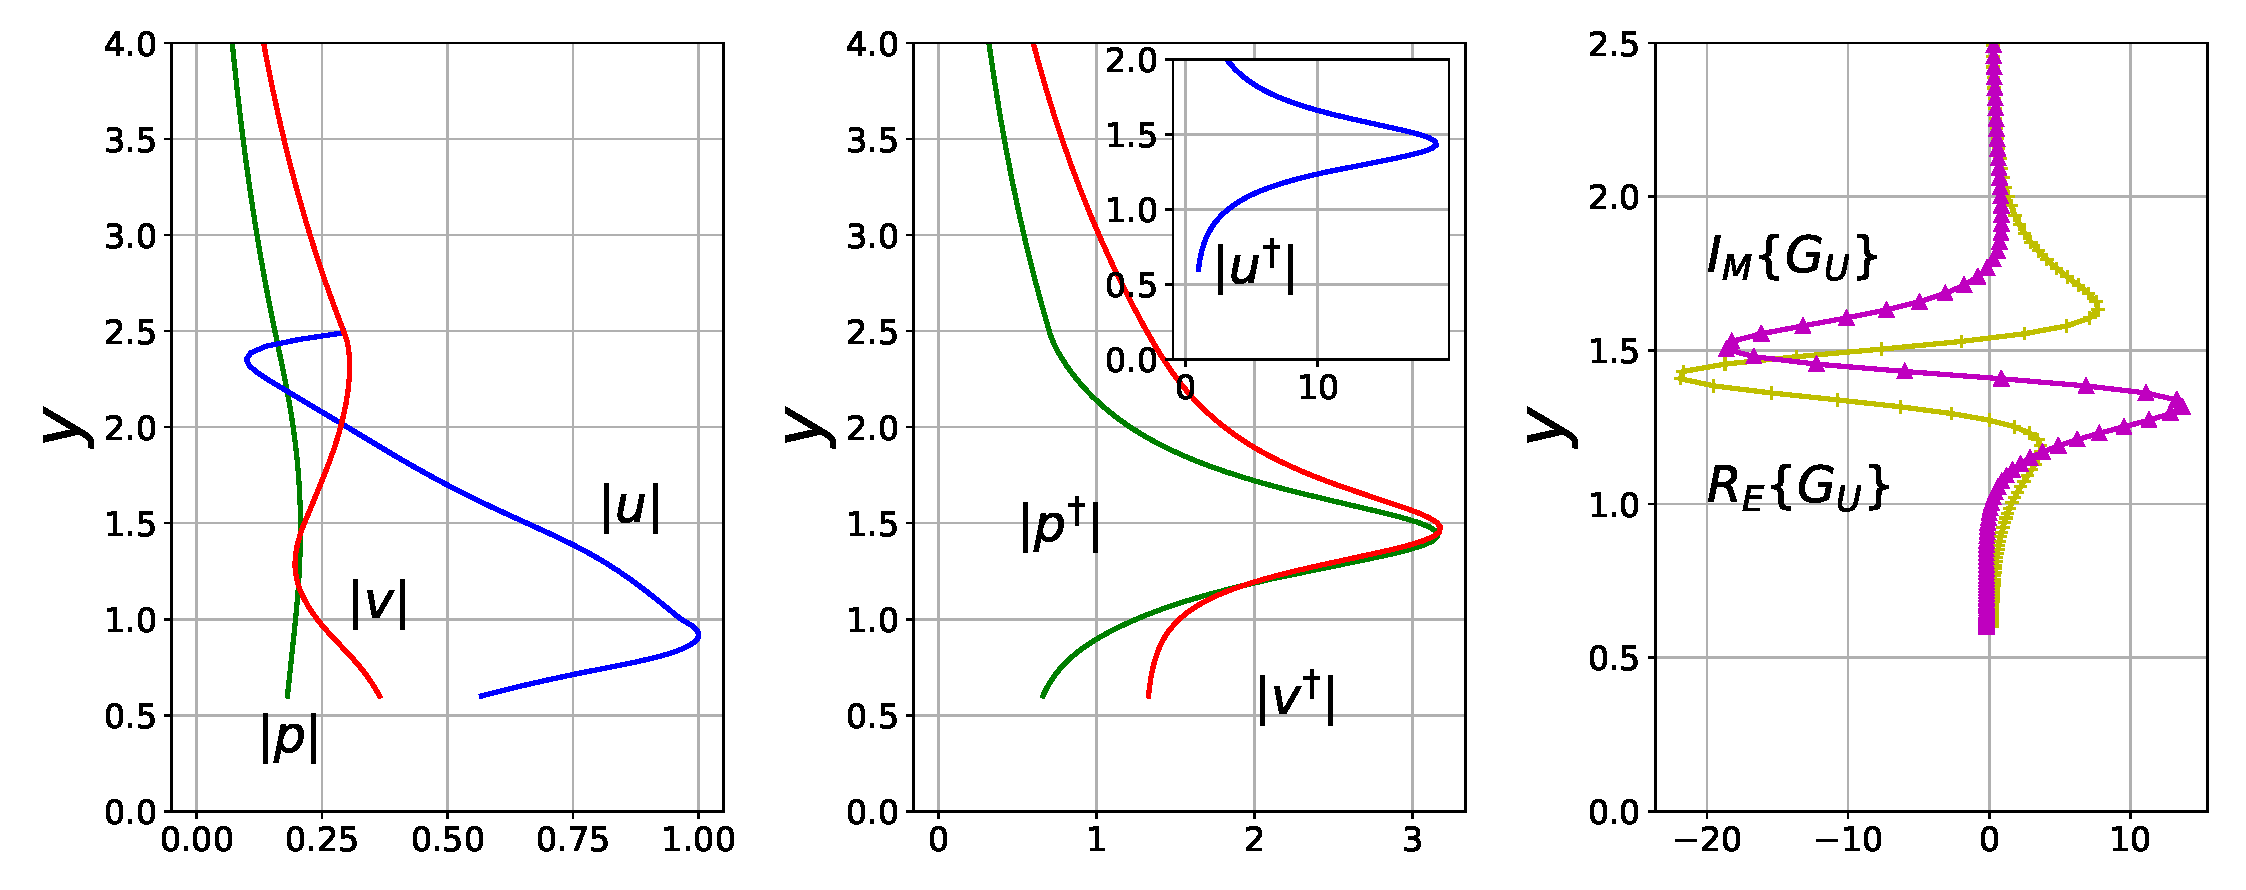
\includegraphics[width=1\linewidth]{chapter_3/figure/7}
	\caption{Left and center frames: moduli of direct and adjoint eigenfunctions; pressure and “adjoint pressure” are drawn with
		dashed lines. Right: real and imaginary parts of the sensitivity function $G_U$ ($\alpha = 0.4790$)}
	\label{fig:7}
\end{figure}

\begin{figure}[H]
	\centering
	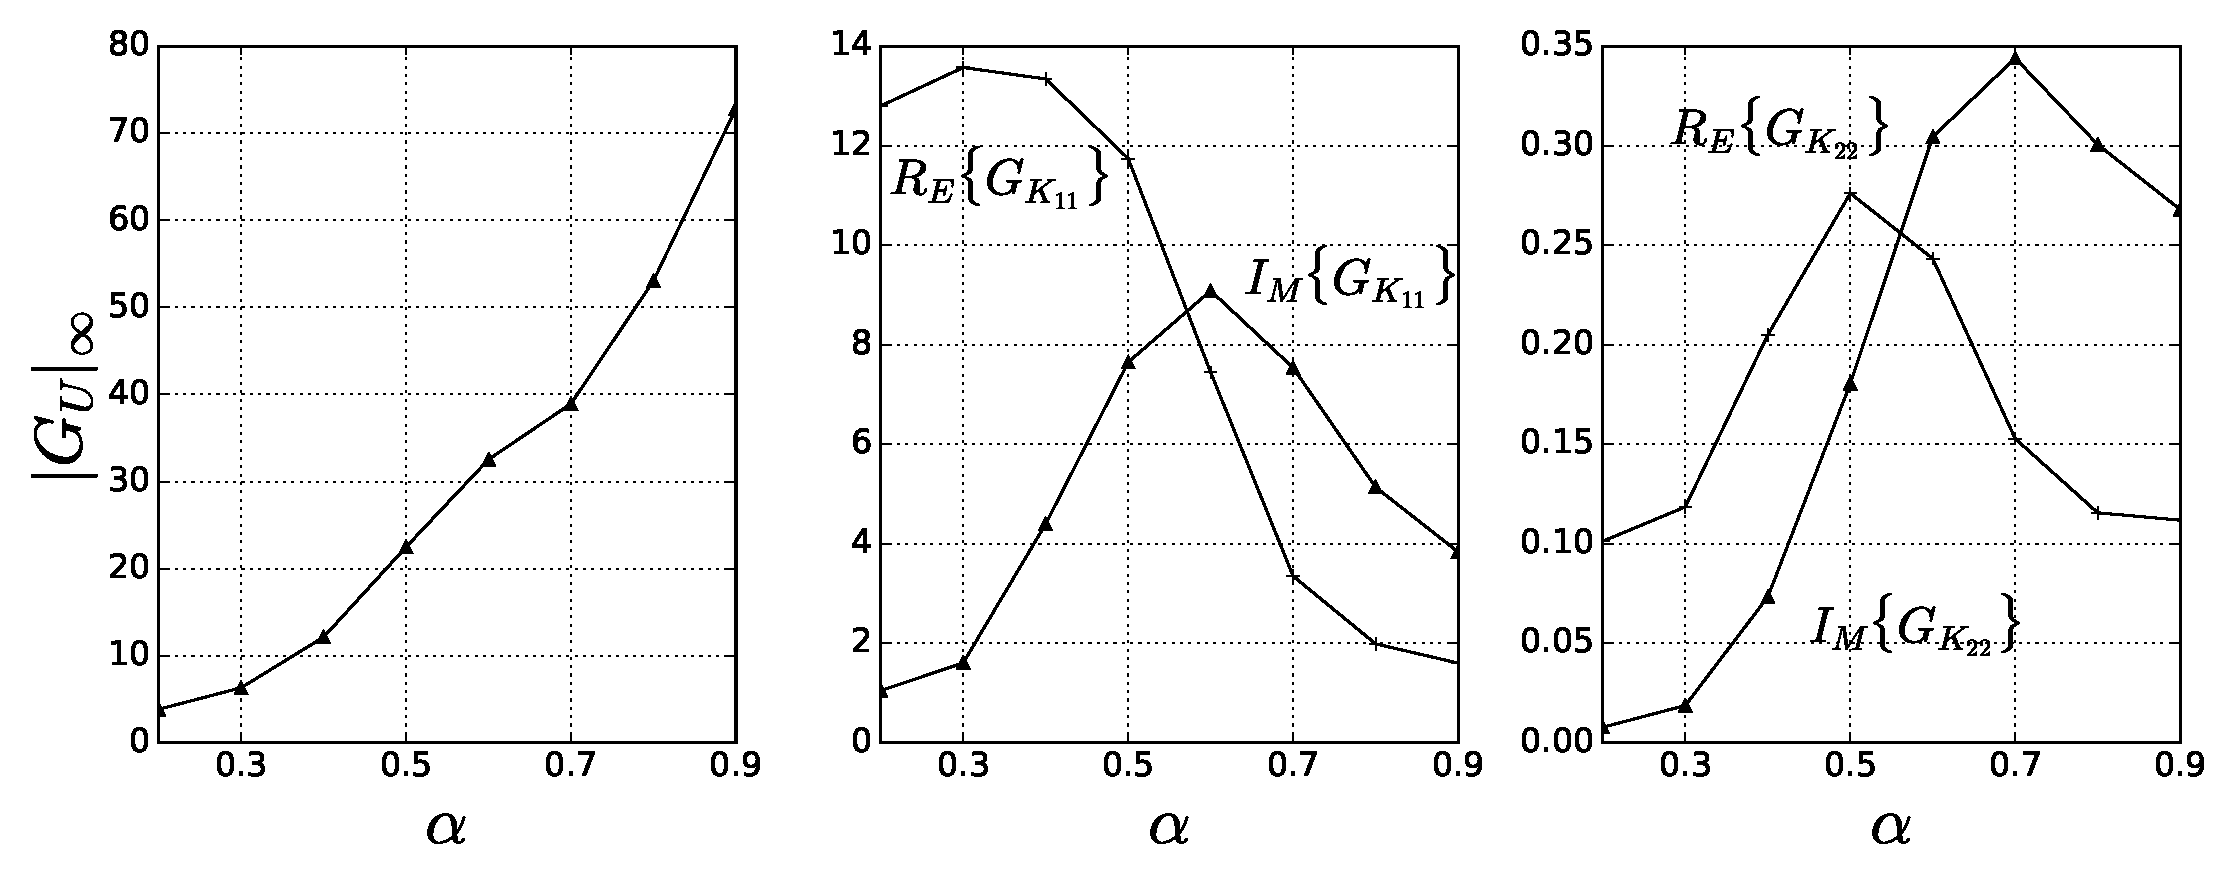
\includegraphics[width=1\linewidth]{chapter_3/figure/8}
	\caption{Case G. Left: infinite norm of $G_U$ for varying $\alpha$. Center and right frames: real and imaginary parts of the sensitivity
		coefficients to variations in the permeability components}
	\label{fig:8}
\end{figure}

smaller and shifted towards a larger y than in the previous inviscid case (cf.\ref{fig:4}, top-right frame).
This can also be appreciated by the inspection of \ref{fig:8} (left); $|G U |_{\infty}$ still grows monotonically with
$\alpha$, but the sensitivity is smaller than that computed earlier (cf. \ref{fig:5}) with either the viscous or
inviscid model (it is actually closer to the viscous sensitivity, as an effect of the interface condition).
Furthermore, it is interesting to observe that both real and imaginary parts of $G_U$ vanish for $y = y|_{itf}$
(cf.\ref{fig:7}, right), and this supports the statement made previously that a small shift in the position
of the effective interface has but a minor influence on the most unstable mode.
The sensitivity coefficients for the two components of the permeability tensors are displayed in
\ref{fig:8} (center and right frames): the present model is more effective to variations in $\mathcal{K}_{11}$ than to $\mathcal{K}_{22}$
as far as modifying the complex eigenfrequency. Significantly, different ranges of wavenumbers
behave differently as far as the variation in $\omega$ is concerned. The frequency $\omega_r$ of long waves (around
$\alpha \approx 0.3$) is more easily modified by acting on $\mathcal{K}_{11}$ (with an almost negligible effect on the growth
rate of the wave); conversely, the growth rate of modes with large values of $\alpha$ is affected efficiently
by variations in the first component of the permeability tensor.


%%%%%%%%%%%%%%%%%%%%%%%%%%%%%%%%%%%%%%%%%%%%%%%%%%%%%%%%%%%%%%%%%%%%%%
\section*{Digression on spatial stability theory and group velocity}
%%%%%%%%%%%%%%%%%%%%%%%%%%%%%%%%%%%%%%%%%%%%%%%%%%%%%%%%%%%%%%%%%%%%%%

Stability problems such as the first one considered in this paper can be approached with the
spatial theory framework, with the wavenumber $\alpha$ complex, its imaginary part being a growth rate,
and the circular frequency $\omega$ a real constant parameter. Let us generalize the sensitivity analysis by
considering, as a first step, $\alpha$ and $\omega$ as complex numbers which can vary. Equation \ref{eq:lagid} contains one
additional term and reads:

\begin{equation}
0 = \delta \langle q^{\dagger}, \mathscr{L} q \rangle = 
\langle q^{\dagger}, \mathscr{L} \delta q \rangle +
\langle q^{\dagger}, \derp{\mathscr{L}}{U}  q \delta U\rangle +
\langle q^{\dagger}, \derp{\mathscr{L}}{C_d}  q \delta C_d\rangle +
\langle q^{\dagger}, \derp{\mathscr{L}}{\omega}  q \rangle \delta \omega +
\langle q^{\dagger}, \derp{\mathscr{L}}{\alpha}  q \rangle \delta \alpha
\label{eq:lagid_spatial}
\end{equation}

To obtain the sensitivities in the spatial problem (for which $\delta \omega = 0$) we now have to solve an adjoint
system similar to \ref{eq:uvp}, where $\omega^{\dagger}$ is replaced by $\omega$ and $\alpha$ by $\alpha^{\dagger}$ . The variation of the wavenumber  $\delta \alpha = 0$ is thus given by:

$$
\delta \alpha =\delta \alpha_r + i \delta \alpha_i= \int_0^{y_{\infty}}  G_U(y) \delta U(y) dy + \int_0^{1}  G_{C_D}(y) \delta C_D(y) dy
$$

the functions $G_U$ and $G_{C_d}$ maintain the same form as in the temporal theory \ref{eq:GCD}, with the direct and
adjoint eigenfunctions which are now normalized by imposing that $N_{\alpha} = -1$, with

$$
N_{\alpha} = \int_0^{y_{\infty}} \left[ \left(U - \dfrac{2i\alpha}{Re}\right) ( \overline{ v^{\dagger}} v +  \overline{ u^{\dagger}} u  )   +  \overline{ p^{\dagger}} u +  \overline{ u^{\dagger}} p  \right] d \; y
$$

Let us now consider a problem in which $U$ and $C_d$ are not allowed to vary, but $\alpha$ and $\omega$ are.
With reference to Equation \ref{eq:lagid_spatial}, with any choice of normalization of direct and adjoint modes, it
is found that $ N_{\omega} \delta \omega = N_{\alpha} \delta \alpha $. Thus, once the adjoint problem is solved, it is possible to accurately
compute the group velocity $c_g$ of any stability problem using the value of $ N_{\omega}$ and $ N_{\alpha}$ , i.e.,

\begin{equation}
c_g := \dfrac{d \omega_r}{d \alpha_r} \approx \dfrac{real(N_{\alpha})}{real(N_{\omega})}
\label{eq:group_vel}
\end{equation}

Note that $c_g$ above is different from the “complex group velocity” $C_g := \dfrac{d \omega}{d \alpha} \approx  \dfrac{N_{\alpha}}{N_{\omega}}$ , and it is also
$c_g \neq real(C_g)$. Relation \ref{eq:group_vel} can be employed in either a spatial or temporal stability analysis and
some representative results (for case G) are provided in Table I with the phase velocity $c_r := \omega_r / \alpha_r$
and the group velocity determined from Equation \ref{eq:group_vel} . The temporal or spatial amplification factors, $\omega_i$ or $-\alpha_i$ , respectively, are also given for all cases using Gaster’s transformation: $\omega_i = - \alpha_i c_g$ .
Two types of errors on the calculation of the group velocity (noted $err$) are given in the table; the top
four values, relative to the temporal theory, are defined as

$$
err = \dfrac{|c_g|_{\ref{eq:group_vel}} - c_g|_{FD}|}{c_g|_{\ref{eq:group_vel}}}
$$

with $c_g|_{FD}$ arising from a first-order finite difference approximation of the group velocity. The
bottom four values are defined by the formula

$$
err = \dfrac{|c_g|_{temporal} - c_g|_{spatial}|}{c_g|_{temporal}}
$$

The relative difference on $c_g$ between temporal and spatial theory is rather low. It has to be kept
in mind, however, that a stability analysis in the spatial framework yields a nonlinear eigenvalue
problem, with a consequent larger numerical system than in the temporal framework; therefore, by
inverting matrices of the same size, the accuracy is expected to be slightly lower. The accuracy of
the growth rate approximated through Gaster’s relationship is also found to be acceptable.

\begin{table}[H]
	\begin{center}
		\begin{tabular}{l|c|c|c|c|c|c|c|c}
			\hline 
			\hline
			Theory & $Re$ & $\alpha_r$ & $\omega_r$ & $-\alpha_i$ & $\omega_i$ & $c_r$ & $c_g$ & $err(\%)$ \\ 
			\hline 
			Temporal & 500 &\textbf{ 0.5}  & 0.4778 & \textit{0.0248} & 0.0254 & 0.9556 & 1.0245 & 0.54 \\ 
			
			& 3450 & \textbf{0.5}  & 0.4601 &\textit{ 0.0413} & 0.0404 & 0.9202 & 0.9797 & 0.06 \\ 
			
			& $10^5$ & \textbf{0.5 } & 0.4514 & \textit{0.0436} & 0.0421 & 0.9028 & 0.9661 & 0.63 \\ 
			
			& $10^9$ &\textbf{ 0.5}  & 0.4508 & \textit{0.0451} & 0.0425 & 0.9016 & 0.9427 & 2.90 \\ 
			
			Spatial & 500 & 0.4993 & \textbf{0.4778} & 0.0248 & 0.0250 & 0.9569 & 1.0100 & 1.41 \\ 
			
			& 3450 & 0.4990 & \textbf{0.4601} & 0.0427 & 0.0404 & 0.9220 & 0.9471  & 3.30 \\ 
			
			& $10^5$ & 0.4996 & \textbf{0.4514} & 0.0449 &  0.0416 & 0.9109 & 0.9371 & 3.46 \\ 
			
			& $10^9$ & 0.4993 & \textbf{0.4508} & 0.0450 & 0.0411 & 0.9028 & 0.9143 & 3.01 \\ 
			\hline 
			\hline
		\end{tabular} 
	\end{center}
	\label{tab:spa_tem}
	\caption{Temporal versus spatial stability, Case G. The model employed
		here is based on a modified Orr-Sommerfeld equation—rather than a system
		based on primitive variables as done in the bulk of the paper—which is
		why the temporal results have slightly larger growth rates $\omega_i$ than those
		displayed in Fig. \ref{fig:2}; this is related to the need of computing numerically
		$d^2 U /dy^2$ and $dC_d /dy$ in the Orr-Sommerfeld-like equation. In italics,
		the growth rates obtained from Gaster’s transformation are reported; the
		parameters imposed in each simulation are indicated with bold characters.
		The solutions for $Re = 10^9$ coincide with those found using the inviscid
		equations.}
\end{table}

The amplitude of the sensitivity functions, $|G_{U} ( y)|$ and $|G_{C_d} (y)|$, in the spatial and temporal
stability frameworks is of same order of magnitude (not shown here) since they are related through
temporal spatial the complex group velocity $C_g$ . It is found that $|{G_U}^{temporal}| \approx |C_g ||{G_U}^{spatial}|$ with $|C_g | \approx c_g \approx 1$ in the
present case.
Obtaining and comparing results in the temporal and spatial stability frameworks, such as in
Table I, is a good means to validate the sensitivity functions and to verify the accuracy of the
computations of the adjoint stability equations.


%%%%%%%%%%%%%%%%%%%%%%%%%%%%%%%%%%%%%%%%%%%%%%%%%%%%%%%%%%%%%%%%%%%%%%
\section{Concluding remarks}
%%%%%%%%%%%%%%%%%%%%%%%%%%%%%%%%%%%%%%%%%%%%%%%%%%%%%%%%%%%%%%%%%%%%%%
We have considered two different models of the flow through a vegetated layer experienc-
ing Kelvin-Helmholtz destabilization. One model is based on the use of a single drag coefficient
to express the force exerted by the vegetation on the fluid, the second considers the canopy as
an orthotropic porous medium and is based on Darcy’s equation with a tensorial permeability \citet{zampogna2016fluid}. 
Both models have advantages and drawbacks. The main advantage of the first model is that the
drag coefficient can be taken to vary across the canopy; whether this positive consideration, based
on macroscopic experimental measurements \citet{ghisalberti2002mixing} \citet{ghisalberti2004limited} \citet{ghisalberti2005mass},  carries over to the stability problem remains to
be established. The second model, applicable to dense porous media, considers two independent
parameters to express the disturbance flow perpendicular and parallel to the rigid dowels forming
the canopy. Such parameters and components of the transversely isotropic permeability tensor K i j
arise from the solution of a local Oseen problem \citet{zampogna2016fluid}. The drawback of the second model is the
fact that an interface (whether real or effective) appears, and adequate matching conditions must
be enforced there. Despite much work since the seminal contribution by \citet{beaver}, a
consensus on the “best” interface conditions between a pure fluid region and a porous medium has
not yet emerged.
The models have been put to test through a classical sensitivity analysis \citet{bottaro2003effect}. Beyond display-
ing stability results which correspond better to those to be expected from available experimental
correlations \citet{raupach1996coherent} \citet{zampogna2016instability}, the anisotropic model is less sensitive to variations in the base flow (with potentially
larger variations in frequency and growth rate of the instability mode for the case of shorter waves).
As far as a direct comparison between $G_{C_d}$ and $G_{\mathcal{K}_{ii}}$ is concerned, this can hardly be made since
the variables represent different objects; in particular, the pressure drop through the canopy depends
directly on $C_d$ and inversely on the permeability. The present results indicate that the anisotropic
model depends significantly on the value of the apparent \citet{zampogna2016fluid} permeability component $\mathcal{K}_{11}$ , whose
evaluation must thus be conducted carefully. This model is also of interest for further developments,
in particular for the study of instabilities developing over waving canopies. Darcy’s law in this latter
case would need to be modified, as described in \citet{mei2010homogenization} and \citet{zampognaMech}.


%%%%%%%%%%%%%%%%%%%%%%%%%%%%%%%%%%%%%%%%%%%%%%%%%%%%%%%%%%%%%%%%%%%%%%%
%\section*{Acknowledgment}
%%%%%%%%%%%%%%%%%%%%%%%%%%%%%%%%%%%%%%%%%%%%%%%%%%%%%%%%%%%%%%%%%%%%%%%
%The authors would like to thank the IDEX Foundation of the University of Toulouse for the
%financial support granted to the last author under the project “Attractivity Chairs.” The computations
%have been conducted at the CALMIP center, Grant No. P1540. The referees are gratefully acknowl-
%edged for their comments leading, in particular, to the correct interpretation of the sensitivity of the
%drag coefficient and to the material in Appendix A.



%%%%%%%%%%%%%%%%%%%%%%%%%%%%%%%%%%%%%%%%%%%%%%%%%%%%%%%%%%%%%%%%%%%%%%%
%\section*{Appendix A: effect of $C_D$ on the mean flow}
%%%%%%%%%%%%%%%%%%%%%%%%%%%%%%%%%%%%%%%%%%%%%%%%%%%%%%%%%%%%%%%%%%%%%%%
%
%In \ref{sec:2ch3} of the paper it is described how the eigenvalue $\omega$ varies as an effect of indepen-
%dent variations of $U$ and $C_d$. However, since $C_d$ is not zero within the canopy and it is used to
%compute the mean flow profile $U$, we should in principle have expressed $\delta U$ as $\delta U = \dfrac{dU}{d C_d} \delta C_d$
%and considered a single sensitivity function ${G^*}_{C_d} = G_{C_d} + \dfrac{dU}{d C_d} G_U$, instead of the two sensitivities given
%in \ref{eq:GCD}. This would have certainly been the appropriate line of action if the mean flow equa-
%tion were issued from exact equations, in which case we should have considered also the adjoint
%of the base flow equation in our variational problem. However, the mean flow model by \citet{ghisalberti2004limited} contains empirical approximations and parameters, and alternative models \citet{singh2016linear}, \citet{zampogna2016instability} —including
%very different ones—have been used successfully in the past to predict the mean field; we have thus
%made the choice, in both \ref{sec:3} and \ref{sec:4}, of considering the mean flow as given, and to take
%independent variations of $U$ and $C_d$ in the stability analysis to assess the effect of modifications in
%either variable.
%If we were to find how much the base flow depends on the drag coefficient in this particular
%problem, we would need to determine the function $U(C_d)$ and take its derivative. Since both $U$
%and  $C_d$ are functions of the space coordinate $y$, the implicit dependence can be found, and we
%have plotted it for one case on the left frame of \ref{fig:9}. Clearly, the function $U = f(C_d)$ is not
%single-valued and therefore the derivative can be calculated only over two separate $U$ (or, equiva-
%lently, $y$) intervals. We have carried out the derivation numerically over each interval, within the
%range $0.3 \leq y \leq 1$, and the result is reported on the right frame of \ref{fig:9}. The filled triangle and
%circle symbols indicate the two y intervals within the canopy.
%We first observe that both the location where $C_d$ is maximum and the shape of the function 
%$U = f(C_d)$ are strongly correlated to the drag law $C_d(y)$, modeled by \citet{ghisalberti2004limited}
%
%
%\begin{figure}[H]
%	\centering
%	\includegraphics[width=1\linewidth]{chapter_3/figure/9}
%	\caption{Case G. Left: mean velocity profile, $U$ , versus the drag coefficient, $C_d$ . Right: first derivative, $dU / d C_d$ . The triangles denote the region $y \in [0.76, 1]$, the filled circles denote the region $y \in [0.3, 0.76]$.}
%	\label{fig:9}
%\end{figure}
%
%through their measurement data (cf. their Figure 7 and Equation (18)). We also notice that the deriv-
%ative $dU/dC_d$ is reasonably small except locally at the point where the derivative of the function is
%not continuous, where it is of order 1. The discontinuity there is however artificial since the function
%$C_d(y)$ given in Equation (18) of \citet{ghisalberti2004limited}, where $C_d$ is divided into a parabolic and a
%linear part, can be easily modified to yield a continuous first derivative at $y = 0.76$ if required, still
%maintaining a mean flow very close to the measured one.



%%%%%%%%%%%%%%%%%%%%%%%%%%%%%%%%%%%%%%%%%%%%%%%%%%%%%%%%%%%%%%%%%%%%%%%
%\section*{Appendix C: comparison between continuous and discrete adjoint eigenfunctions}
%%%%%%%%%%%%%%%%%%%%%%%%%%%%%%%%%%%%%%%%%%%%%%%%%%%%%%%%%%%%%%%%%%%%%%%
%
%The discretization operation transform the operator $\mathcal{L}$ into a matrix $\mathbf{A}$ and of course do the same things to the unknown functions that becomes vectors.
%
%\begin{table}[H]
%	\begin{center}
%		\begin{tabular}{|c|c|}
%			\hline 
%			continuous & discrete \\ 
%			\hline 
%			$\mathcal{L}$ & $\mathbf{A}$ \\ 
%			\hline 
%			$q$ & $\hat{q}$ \\ 
%			\hline 
%		\end{tabular} 
%	\end{center}
%\end{table}
%
%This has a serious and most often hidden repercussion in th approach to solve the adjoint equations.
%
%As above stated the derivation of the adjoint equation start with the enforcing of the Lagrange identity:
%
%\begin{equation}
%\langle q; \mathcal{L} q \rangle = \langle {\mathcal{L}}^{\dagger} q^{\dagger} ; q \rangle
%\end{equation}
%
%where the scalar product $ \langle ;\rangle$ is defined in our case as:
%
%\begin{equation}
%\langle a ; b\rangle = \int_{0}^{y_{\infty}} \overline{a} \cdot b dy \approx \sum_{i=1}^N \sum_{j=1}^N {\hat{\overline{a}}_i}^T w_{i,j} {\hat{b}_j} = {\hat{\overline{a}}_i}^T \mathbf{M} {\hat{b}_j} =  \langle a ; b\rangle_{\mathbf{M}}
%\label{eq:scalr_prod}
%\end{equation}
%
%Is it clear from equation \ref{eq:scalr_prod} that the scalar product takes two different forms in the continuous and in the discrete case.
%In fact in the discrete case is mandatory to introduce the quadrature rule weights $w_{i,j}$ of the chosen discretization.
%$\mathcal{M}$ is the matrix representation of the weights and is symmetric and positive defined.
%
%In order to compute and solve the adjoint equation one could proceed as follow:
%
%\begin{itemize}
%	\item The direct problem is defined in the continuous space as $\mathcal{L} q = 0$
%	\item Chose a discretization (FEM, FD, Chebychev polynomials...) and transform the above problem in a discrete one $\mathbf{A} \hat{q}$
%	\item Solve it to obtain the discrete version of the eigenfunctions $\hat{q}$
%	\label{continuous}
%\end{itemize}
%
%For the adjoint problem on should at first compute the adjoint operator, this can be done using the Lagrangian identity at a continuous level:
%
%\begin{equation}
%\begin{split}
%\langle q; \mathcal{L} q \rangle =& \langle {\mathcal{L}}^{\dagger} q^{\dagger} ; q \rangle \\
%\Rightarrow \int_{0}^{y_{\infty}} \overline{q^{\dagger}} \; \mathcal{L} q  \; dy =& \int_{0}^{y_{\infty}} \overline{ {\mathcal{L}}^{\dagger} q^{\dagger}}  \; q  \; dy 
%\end{split}
%\end{equation}
%
%From the last equation starting from the left part is it possible after some manipulation to retrieve the form on the right part and so find the formulation of the adjoint operator.
%
%It is important to pinpoint that in the above equation the  scalar product $ \langle a ; b\rangle$ is enforced at a continuous level.
%
%And now to solve the adjoint system the procedure \ref{continuous} can be used changing the direct system with the adjoint one.
%The above way of computing the adjoint and solve the system is called \textbf{continuous approach}.
%
%To summarize this approach one can straight forward solve th direct problem computationally, mathematically find the adjoint operator using the continuous scalar product and the Lagrange identity and then discretize the adjoint problem and solve it computationally.
%This is why the \textbf{continuous approach} is sometimes known as derive than discretize.
%And the stability and accuracy problems derive directly from the fact that we discretize the problem two times (the direct first and than the adjoint).
%
%
%On the contrary in the \textbf{discrete approach} the scalar product \ref{eq:scalr_prod} is enforced at the discrete level in order to use the already discretized direct equation to retrive the adjoint system at a discrete level, to limit the computational errors.
%
%\begin{equation}
%\begin{split}
%\langle q^{\dagger}; \mathcal{L} q \rangle =& \langle {\mathcal{L}}^{\dagger} q^{\dagger} ; q \rangle \\
%\Rightarrow \overline{\hat{q}^{\dagger}}^T \mathbf{M} \mathbf{A} \hat{q}  =& \left( \overline{{\mathbf{A}}^{\dagger} \hat{q}^{\dagger}} \right)^{T} \mathbf{M} \hat{q} \\
%\Rightarrow \mathbf{M} \mathbf{A}  =&  {\overline{\mathbf{A}^{\dagger}}}^T \mathbf{M} \\
%\Rightarrow {\mathbf{A}}^{\dagger}  =&  \mathbf{M}^{-1} \mathbf{\overline{A}}^T \mathbf{M}
%\end{split}
%\end{equation}
\chapter{Effect of geometrical parameters and inertia on the apparent permeability tensor in fibrous porous media}
\label{ch:4}


\chapquote{Before we work on artificial intelligence, why don’t we do something about natural stupidity?}{}{Steve Polyak}


%%%%%%%%%%%%%%%%%%%%%%%%%%
\section{Introduction}
%%%%%%%%%%%%%%%%%%%%%%%%%%

Since Darcy's original formulation (\citet{darcy}), which relates the flow rate through a porous bed to the pressure drop across the bed's sides, many corrections have been made to account, for example, for viscous effects (\citet{brinkman}) or for the consequences of inertia (\citet{forchheimer}).  
All of the cited works are of empirical nature, but the volume averaged methods (VANS) has been able to recover all of these
formulations rigorously starting from the Navier-Stokes equations (\citet{whitaker2013method}).

As already seen in chapter 2, the VANS theory requires the knowledge of a number of terms, most notably, in the case of an isotropic porous bed, a permeability coefficient and a Forchheimer coefficient. Initial efforts in defining these terms were based on a combination of physical reasoning and measurements, leading to  expressions known as the Kozeny-Carman \citet{kozeny, carman} and the Ergun \citet{ergun} correlations. These approaches do not consider microstructural or geometrical features of the porous bed and are often restricted to simple unidirectional flows. In the present work we are concerned with a transversely isotropic material composed by parallel fibers of circular cross-section, with one axis of symmetry, $(O,x_3)$; in such materials the permeability is a diagonal tensor
with the component in the direction parallel to the fibers greater than those along the transverse axes. For such an arrangement
we will investigate, in this chapter, the effects of both the direction of the forcing pressure gradient and inertia. When the latter effect is present,
embodied by a Reynolds number $Re_d$, based on mean velocity through the medium and fibers' diameter, exceeding an order one threshold, 
the permeability is no more simply defined upon geometrical properties. This extended permeability, which arises from a well-defined closure problem \eqref{eq:M_problem}, is then called \emph{apparent permeability}.

The influence of the geometry of the solid inclusions has been addressed previously by \citet{yazdchi2011} for arrays of cylinders 
in both square and hexagonal (or staggered) patterns, with the cylinders' section which can vary in shape. The results, in the 
two-dimensional and low Reynolds number limits, demonstrate the dependence of the  permeability component along the flow direction to both 
the porosity and the direction of the macroscopic pressure gradient. The direction of the pressure gradient is found to have a weak effect 
for beds of medium-high porosity ($\varepsilon>0.7$) and a stronger dependence appears upon the geometry of the solid inclusions. 
%An interesting observation made by \citet{yazdchi2011} concerns the relation between the angle of the staggered cell arrangement 
%and the permeability, particularly for medium-high porosities.

%In \citet{lasseux} the authors study the problem of the inertia correction on the Darcy law (Forchheimer tensor), and its relation 
%with the Reynolds number and the orientation of the mean pressure gredient.
The influence of the Reynolds number on the permeability and on the Forchheimer correction has been presented in a number of papers (\citet{firdaouss1997nonlinear}, \citet{penha2011computing} and \citet{edwards1990}). These authors show that, for arrays of fibers, the apparent permeability decreases with the increase of the Reynolds number, and the rate of this decrease depends on the geometry of the array;
also, the Reynolds number is found to have a stronger influence on the apparent permeability when the medium is highly porous.
The results of the work by \citet{edwards1990} agree with those by \citet{zampogna2016fluid} and with our own work (as shown later), all for
the case of cylindrical fibers, although some issues remain on the persistence of steady solutions in the simulations by \citet{edwards1990} 
in cases for which a limit cycle should have set in. A fully three-dimensional porous medium, more complex than those discussed so far, 
has been considered by \citet{soulaine2014}, confirming the decreasing trend of the apparent permeability with the Reynolds number. 

Another contribution which deserves mention is that by \citet{lasseux}; they have computed the permeability tensor 
for various Reynolds numbers, in a two-dimensional geometry with cylinders of square cross-section.
Forcing the flow along the main symmetric directions of the fiber, the same authors have identified different regimes:
\begin{itemize}
	\item a creeping flow regime for $ 0 < Re_d < 10^{-3}$, without Forchheimer terms;
	\item a weak inertia regime for $10^{-3} < Re_d < 1$, with the Forchheimer correction quadratic in $Re_d$; 
	\item a strong inertia regime for $1 < Re_d < 10$, where the Forchheimer correction is linear with the Reynolds number; 
	\item a turbulent regime, for  $Re_d > 10 $, with the Forchheimer correction again quadratic with the Reynolds number.
\end{itemize}  
The boundaries between the different regimes are specific to the geometrical arrangements and to the porosities being considered; 
a step forward in rendering (some of) these boundaries rigorous and independent of the arrangement of the pores, through the definition 
of a Reynolds number which accounts for a "topological" coefficient, has been recently made by \citet{pauthenet}. 
For the purposes of the present paper, we must retain that \citet{lasseux} have parametrized the Forchheimer correction with the Reynolds 
number, and have found that the inertial correction is orders of magnitude smaller than the Darcy's term, at least before the turbulent 
regime sets in. Moreover, \citet{lasseux} have studied how a Forchheimer tensor, $\mathbf{F}$, depends upon the direction of the
macroscopic forcing term with respect to the orientation of the square cross-section of the fibers, for  $Re_d$ up to 30.
It is concluded that a deviation angle, $\gamma$, exists between the direction of the pressure gradient and that of the mean flow,
because of the fibers' geometry. Finally, the inertial correction is strongly influenced by the orientation
of the driving pressure gradient, and the Forchheimer tensor $\mathbf{F}$ is not symmetric (in fact the off-diagonal components 
are found to be inversely proportional to the diagonal terms, and symmetric with respect to rotations about the diagonal axis of 
the square, i.e. the direction at $45^\circ$ in the $x_1 - x_2$ plane).

The effect of variations in the forcing angle, with restrictions to angles in the $x_1 - x_2$ plane, is also examined by 
\citet{soulaine2014} with conclusions in qualitative agreement with those of  both the contribution just cited and our results  
described further below. In all cases, the off-diagonal components of the apparent permeability tensor are small and the diagonal 
components display but a small variation upon rotation of the driving pressure gradient.


Here we want to show how the direction of the macroscopic pressure gradient, the porosity and the Reynolds number can 
modify the Darcy and Forchheimer closures arising from a VANS model of a fibrous porous medium. We will consider a three-dimensional 
unit cell for the microscopic model, with a generic forcing 
whose direction is defined by two Euler angles. Given the formidable space of parameters, some representative results are first
shown and discussed. Response surfaces in the space of parameters are then identified by the use of a metamodel based on Kriging 
interpolation.
They represent an extremely useful data base which can be afterward used in macroscopic simulations of 
flows through bundles of fibers of varying orientation and porosity.




%%%%%%%%%%%%%%%%%%%%%%%%%%%%%%%%%%%%%%%%%%%%%%%%%%%%%

\section{The Volume-Averaged Navier-Stokes (VANS) method}

%%%%%%%%%%%%%%%%%%%%%%%%%%%%%%%%%%%%%%%%%%%%%%%%%%%%
\label{sec:2ch4}

%%%%%%%%%%%%%%%%%%%%%%%%%%%%%%%%%%%%%%%%%%
%
%\subsection{A brief description of the method}
%
%%%%%%%%%%%%%%%%%%%%%%%%%%%%%%%%%%%%%%%%%%
%
%
The system under investigation consists of an incompressible Newtonian fluid which flows through a rigid porous medium. The governing equations valid at the microscale are:

\begin{eqnarray*}
	\begin{cases}
\dfrac{\partial \vb}{\partial t} + \vb \cdot \nabla \vb = -\frac{1}{\rho_{\beta}} \nabla \pb + \nub \nabla^2  \vb  + \mathbf{f} \\
\nabla \cdot \vb = 0 
	\end{cases}
\label{eq:ns_f}
\end{eqnarray*}

where $\vb$, $\pb$, $\rho_{\beta}$ and $\nub$ stand, respectively, for  the velocity, the pressure, the density and the kinematic viscosity of the fluid.
The right-hand side term, $\mathbf{f}$, is a force (per unit mass) which drives the fluid motion and can be interpreted as the macroscopic pressure gradient acting on the system.
%
%\begin{figure}[H]
%	\centering
%	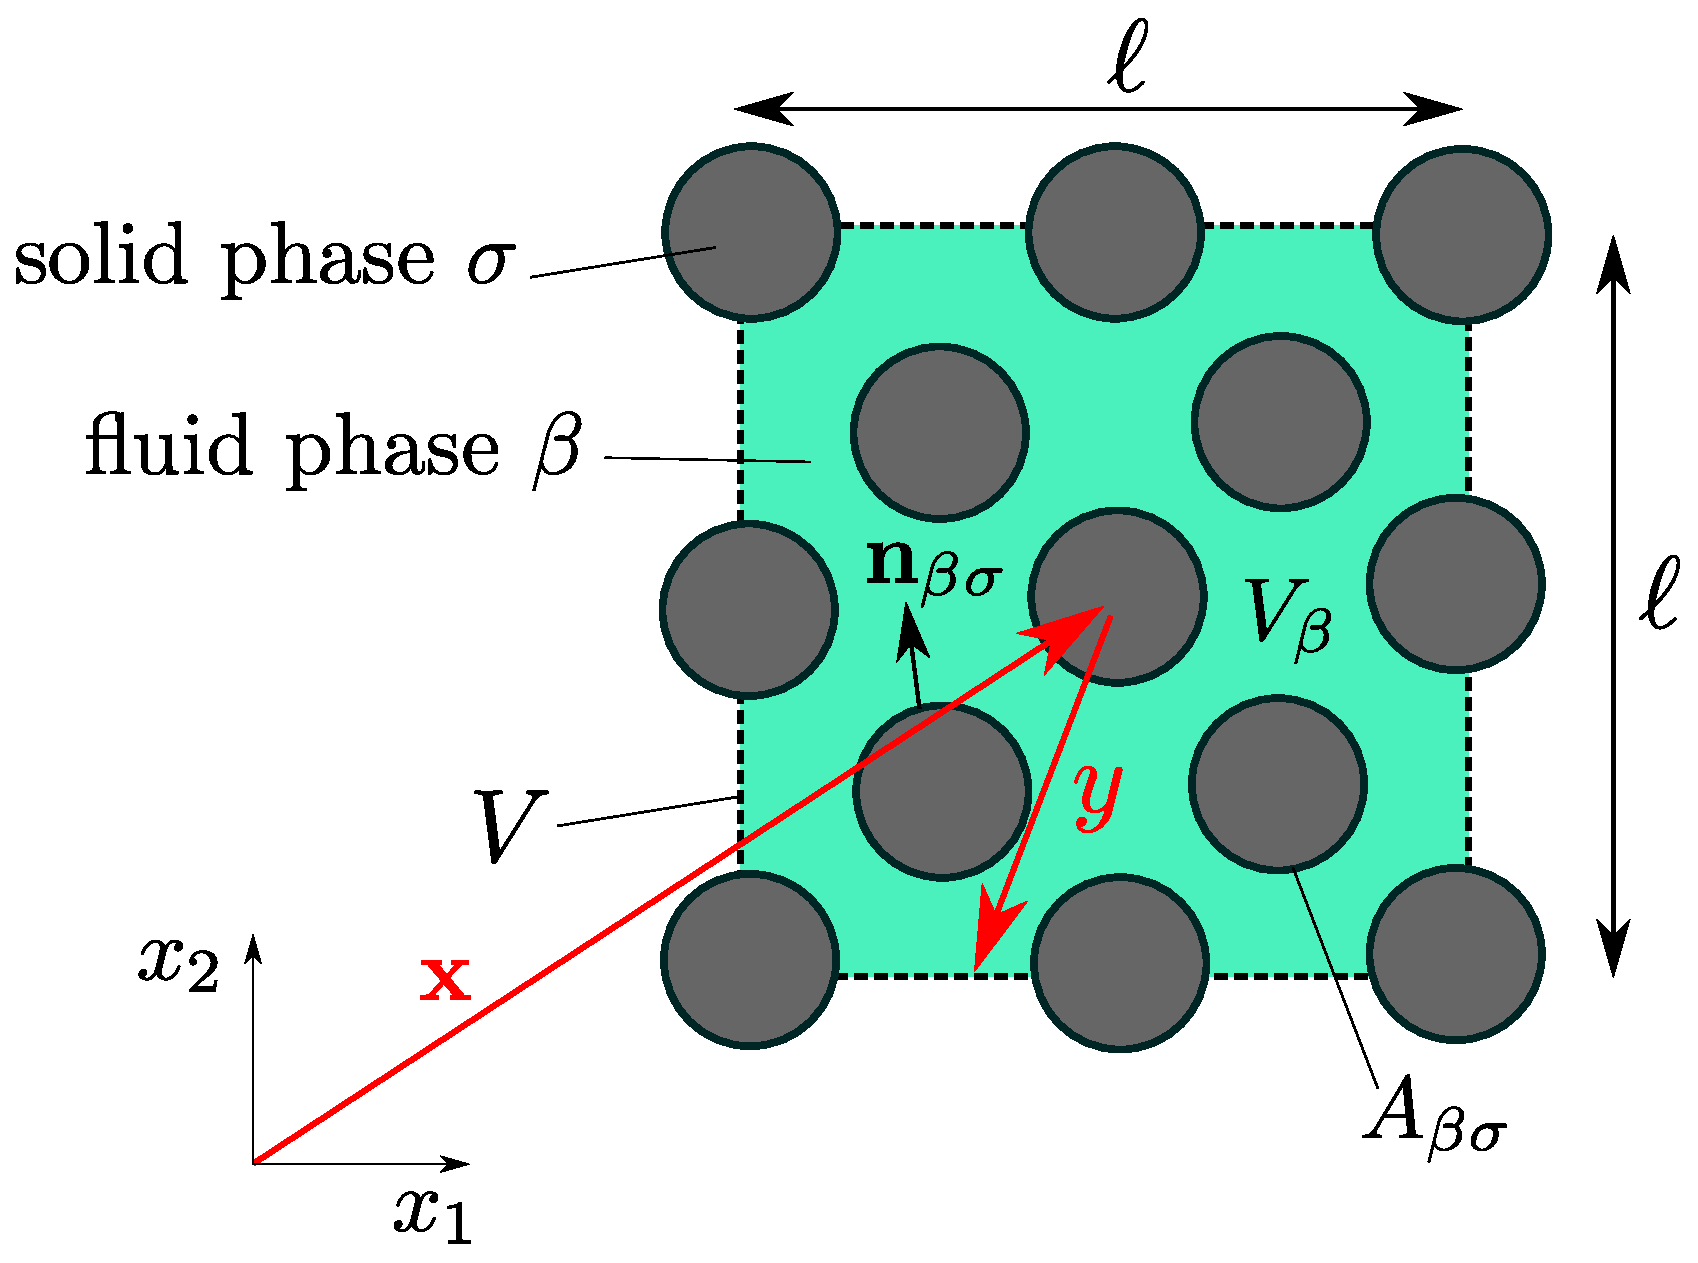
\includegraphics[width=0.8\linewidth]{chapter_4/figure/REV}
%	\caption{Illustration of the REV concept.}
%	\label{fig:rev}
%\end{figure}
%
%
%The concept of Reference Elementary Volume (REV) of the porous medium is classically introduced in the framework of the VANS approach.
%An example of REV  is depicted on figure \ref{fig:rev}, together with relevant notations (volume shape and size, indication of the fact that the normal unit vector is directed from the fluid to the solid phase, centroid $\rm {\bf{x}}$ of the REV). The REV represents  the domain over which the    microscopic problem is solved; its size is defined so as to contain all the microscopic features of the flow. 
%As a rule of thumb, the REV is the smallest  fluid domain over which   periodic boundary conditions can be applied.
%
%
%In the computational domain, any flow variable  $\phi$ can be decomposed into an intrinsic average part $\meani{\phi}$ plus a perturbation $\tilde{\phi}$, as:
%$$  \phi = \meani{\phi} + \tilde{\phi}.$$
%The intrinsic average is defined with an integration carried out only on the fluid phase \citet{whitaker2013method}:
%\begin{equation}
%\meani{\psi_{\beta}} = \dfrac{1}{\volb} \int_{\volb} \psi_\beta (\mathbf{x}) d \volb.
%\label{eq:avg_intrinsic}
%\end{equation}
%Applying such an operator to equations \eqref{eq:mom} and \eqref{eq:cont}, and following \citet{whitaker1996forchheimer} we have:
%$$
%\dfrac{\partial \vbmi}{\partial t} + \vbmi \cdot \nabla \vbmi = -\frac{1}{\rho_{\beta}} \nabla \pbmi + \nu_\beta \nabla^2 \vbmi + \, \mathbf{f} \, + 
%$$
%\begin{equation}
%\dfrac{1}{\volb} \int_{A_{\beta \sigma}}  ( - \frac{\pbt}{\rho_\beta} \mathbf{I} + \nub \nabla \vbt ) \cdot  \mathbf{n}_{\beta \sigma} dA,
%\label{eq:darcy_forch}
%\end{equation}	
%\begin{equation}
%\nabla \cdot \meani{\vb} = 0,
%\label{eq:cont_vans}
%\end{equation}	
%upon neglecting in equation \eqref{eq:darcy_forch} the sub-REV scale dispersion term (linked to the $\left< \vbt \vbt \right>^{\beta}$ term) which is often small in porous media flows \citet{brugem_phd}.
%
In chapter 2 we have already shown how the above equations can be homogenized and a new set of equations, valid at the macroscale, can be retrieved.
The macroscale system \eqref{eq:vans_mom_1} introduce the surface integral term:
$$\mathbf{F}^{\textit{m}} = \dfrac{1}{V} \displaystyle \int_{A_{\beta \sigma}} \left(-\dfrac{\pbt}{\rho_{\beta}} \mathbf{I}  + \nub \nabla \vbt \right)\cdot \nbs \;dA, $$

that we have discussed in chapter 2 section \ref{ch:closure_fm}. This term is close by means of the equation \eqref{eq:closure_final} that we recall here:

\begin{equation}
\mathbf{F}^m \approx \mathbf{F}^M = - \nub \varepsilon \mathbf{H}^{-1} \cdot \meani{\vb}
\label{eq:closure_model}
\end{equation}

%$\mathbf{F}^{\textit{M}}$, must be used to replace $\mathbf{F}^{\textit{m}}$ in the governing equation. Such a model is often based on a permeability tensor, $\mathbf{K}$, and a Forchheimer tensor, $\mathbf{F}$, and reads:
%\begin{equation} 
%\mathbf{F}^{\textit{M}} = - \nub \mathbf{K}^{-1} (\mathbf{I} + \mathbf{F})\vbmi,
%\label{eq:macroscale} 
%\end{equation}
%so that the system is closed by imposing
%\begin{equation}
%\mathbf{F}^{\textit{m}} = \mathbf{F}^{\textit{M}}.
%\label{eq:closure_KF} 
%\end{equation}


The two terms $\mathbf{F}^m$ and $\mathbf{F}^M$ can be interpreted as the force that the fluid exert on the solid structure of the porous medium. The two formulations are different only in the way of computing the force, the former one uses the miscroscopic representation and the latter the macroscopic one.
The drag force $\mathbf{F}^{\textit{m}}$ computed by direct numerical simulations (DNS) with account of all individual pores will be later compared to the model based on the permeability and Forchheimer tensors (whose equations are given below).
This is just a useful exercise to demonstrate consistency of the approach and accuracy of the numerical simulations; it does nothing else since, as briefly described below, to derive the Forchheimer tensor the microscopic velocity field must be known anyhow.  Nonetheless, knowledge of the behavior of these tensors (or, equivalently, of the related apparent permeability) might prove both useful and instructive, in particular should one wish to extend the range of applicability of the model to cases for which the microscopic solution is not available.

The core of the VANS approach consists in the identification of the permeability and Forchheimer tensors. This problem, referred to as the closure problem, is discussed at length in paragraph \ref{ch:closure_fm}.
The two different tensors $\mathbf{K}$ and $\mathbf{F}$  can be computed by means by the two differential problems \eqref{eq:D_problem} and \eqref{eq:M_problem} reported here and discussed in detail in chapter 2.

\begin{eqnarray*}
\begin{cases}
0 = -\nabla \mathbf{d} + \nabla^2 \mathbf{D} +\mathbf{I},\\
\nabla \cdot \mathbf{D} = 0,  \\
\mathbf{D} = 0 \quad \textrm{at} \; A_{\beta \sigma}, \\
\mathbf{d}(\mathbf{x} +\ell_i) = \mathbf{d}(\mathbf{x}), \qquad \mathbf{D}(\mathbf{x} +\ell_i) = \mathbf{D}(\mathbf{x}), \qquad i=1,2,3 , \\
\meani{\mathbf{D}} = \varepsilon^{-1} \mathbf{K}.
\end{cases}
\end{eqnarray*}

The second closure problem differs from the first only for the presence of a linearised convective term 
in which the microscopic velocity obtained from the DNS, $\vb$, is used as an input.  This of course implies knowledge of the microscopic velocity field. A Oseen-like approximation which relaxes this constraint has been proposed by \citet{zampogna2016fluid}.

\begin{eqnarray*}
\begin{cases}
\dfrac{\vb}{\nub} \nabla \mathbf{M} = -\nabla \mathbf{m} + \nabla^2 \mathbf{M} +\mathbf{I},\\
\nabla \cdot \mathbf{M} = 0,  \\
\mathbf{M} = 0 \quad at \; A_{\beta \sigma}, \\
\mathbf{m}(\mathbf{x} +\ell_i) = \mathbf{m}(\mathbf{x}), \qquad \mathbf{M}(\mathbf{x} +\ell_i) = \mathbf{M}(\mathbf{x}), \qquad i=1,2,3 ,\\
\meani{\mathbf{M}} = \varepsilon^{-1} \mathbf{H}.
\end{cases}
\label{eq:h_model}
\end{eqnarray*}


The closure problems reflect the structure of the solution of the two system \eqref{eq:D_problem} and \eqref{eq:M_problem}. In particular, the solution of the former depends only on the geometry of the porous medium so that the permeability tensor $\mathbf{K}$ is symmetric. This is not the case for $\mathbf{H}$, because of the effect of the microscopic velocity amplitude and direction.  Clearly, the solution of system \eqref{eq:M_problem} tends to that of \eqref{eq:D_problem} when $Re_d \rightarrow 0$. 


%%%%%%%%%%%%%%%%%%%%%%%%%%%%%%%%%%%%%%%%%%%%%%%%%%%%%%%%%%%%%%
%%
%%\subsubsection{Closure problems for $\mathbf{K}$ and $\mathbf{F}$}
%%
%%%%%%%%%%%%%%%%%%%%%%%%%%%%%%%%%%%%%%%%%%%%%%%%%%%%%%%%%%%%%%
%
%
%The core of the VANS approach consists in the identification of the permeability and Forchheimer tensors. This problem, referred to as the closure problem, is discussed at length by \citet{whitaker1986flow,whitaker1996forchheimer}.  He derives two partial differential equation systems, the first valid in the zero Reynolds number limit (system \eqref{eq:K_closure} below), while the second applies when inertial terms are not negligible (system \eqref{eq:F_closure1}).
%
%
%
%In the first system of equations   a three component vector $\mathbf{d}$  and  a $3 \times 3$ tensor  $\mathbf{D}$ are introduced.
%This system  can be divided into  three separate independent problems which resemble a forced Stokes problem where each component of $\mathbf{d}$ and the corresponding row of  $\mathbf{D}$  play, respectively, the role of a pressure and a velocity field. Together with the periodic  boundary conditions, the problem reads: 
%\begin{equation}
%\begin{cases} 
%0 = -\nabla \mathbf{d} + \nabla^2 \mathbf{D} + \mathbf{I},\\ 
%\nabla \cdot \mathbf{D} = 0, \\ 
%\mathbf{D} = 0 \qquad {\rm on }  \qquad A_{\beta \sigma},\\
%\mathbf{d}(\mathbf{x} + \ell_i) = \mathbf{d}(\mathbf{x}), \qquad 
%\mathbf{D}(\mathbf{x} + \ell_i) = \mathbf{D}(\mathbf{x}) \qquad i = 1,2,3.
%\end{cases} 
%\label{eq:K_closure}
%\end{equation}
%The permeability tensor is found by applying  the intrinsic average on the $\mathbf{D}$ tensor, i.e.
%$\mathbf{K} = \varepsilon \; \meani{\mathbf{D}}$  and, in the Stokes regime, it is
%\begin{equation}
%\mathbf{F}^{\textit{M}} = - \nub \mathbf{K}^{-1} \vbmi.
%\end{equation}
%
%The second closure problem differs from the first only for the presence of a linearised convective term 
%in which the microscopic velocity obtained from the DNS, $\vb$, is used as an input.  This of course implies knowledge of the microscopic velocity field. A Oseen-like approximation which relaxes this constraint has been proposed by \citet{zampogna}.
%
%The new unknowns are a  vector and a tensor called, respectively,   $\mathbf{m}$  and  $\mathbf{M}$, with  the same meanings of $\mathbf{d}$ and 
%$\mathbf{D}$.
%The system reads:
%\begin{equation}
%\begin{cases} 
%\dfrac{1}{\nub} \vb \cdot \nabla \mathbf{M} = -\nabla \mathbf{m} + \nabla^2 \mathbf{M} + \mathbf{I},\\ 
%\nabla \cdot \mathbf{M} = 0, \\ 
%\mathbf{M} = 0  \qquad {\rm on } \qquad A_{\beta \sigma}, \\
%\mathbf{m}(\mathbf{x} + \ell_i) = \mathbf{m}(\mathbf{x}), \qquad 
%\mathbf{M}(\mathbf{x} + \ell_i) = \mathbf{M}(\mathbf{x}) \qquad i = 1,2,3.
%\end{cases} 
%\label{eq:F_closure1}
%\end{equation}
%The average  of the tensor $\mathbf{M}$  multiplied by the porosity is the \textit{apparent permeability}, 
%$\mathbf{H}= \varepsilon \; \meani{\mathbf{M}}$. When inertia is important equation \eqref{eq:macroscale}  can be written as 
%\begin{equation}
%\mathbf{F}^{\textit{M}} = - \nub \mathbf{H}^{-1} \vbmi,
%\end{equation}
%\noindent as shown by \citet{whitaker1996forchheimer}.
%
%Two remarks are in order at this point.
%First, the equations in the closure problem \eqref{eq:F_closure1} are time-independent because the microscopic velocity $\vb$ is a solution of a stationary DNS.  Thus, the Reynolds number should be sufficiently small for unsteady effects not to be present. Should the wake behind a solid inclusion display regular or irregular temporal oscillations, the equations of system \eqref{eq:F_closure1} may be used, as an
%approximation, by replacing the instantaneous velocity in the REV with its time-averaged distribution.  This case is however not of present concern.
%Secondly, the closure problems reflect the structure of the solution of the two system \eqref{eq:K_closure} and \eqref{eq:F_closure1}. In particular, the solution of \eqref{eq:K_closure} depends only on the geometry of the porous medium so that the permeability tensor $\mathbf{K}$ is symmetric. This is not the case for $\mathbf{H}$, because of the effect of the microscopic velocity amplitude and direction.  Clearly, the solution of system \eqref{eq:K_closure} tends to that of \eqref{eq:F_closure1} when $Re_d \rightarrow 0$. 
%



%%%%%%%%%%%%%%%%%%%%%%%%%%%%%%%%%%%%%%%%%%%%%%%%%%%%%%%%%%%%%%

\section{Validation and setup }

%%%%%%%%%%%%%%%%%%%%%%%%%%%%%%%%%%%%%%%%%%%%%%%%%%%%%%%%%%%%%%%


In this section the numerical methodology, the parameters, the setup and the validation for some reference cases are given.


%%%%%%%%%%%%%%%%%%%%%%%%%%%%%%%%%%%%%%%%%%%%%

\subsection{Computational domain}

%%%%%%%%%%%%%%%%%%%%%%%%%%%%%%%%%%%%%%%%%%%%%


The geometry used for the base REV is shown in figure \ref{fig:cell_3d}: a cylindrical inclusion is present at the center of the REV and four quarters of cylinders are situated at the corners. The lateral length of the cubic envelop is $\ell$, which is used as length scale for the microscopic problem; the diameter $d$ of the cylinders is adapted as a function of the desired porosity $\varepsilon$, ratio between the fluid volume over the total REV volume ($\ell^3$). 

The  forcing term $\mathbf{f}$ of the DNS  is a vector whose direction is defined by two Euler angles, with rotations of the form:  $\theta \ \mathbf{e_3} + \phi \ \mathbf{e_2}^{I}$ (cf. figure \ref{fig:cell_3d}). Its amplitude is set a priori and is connected to the Reynolds number, $Re_d$, defined with the mean velocity over the REV and the fiber diameter, $d$. $Re_d$ is a result of the calculations, once the mean velocity is evaluated.

\begin{figure}[h]
	\centering
	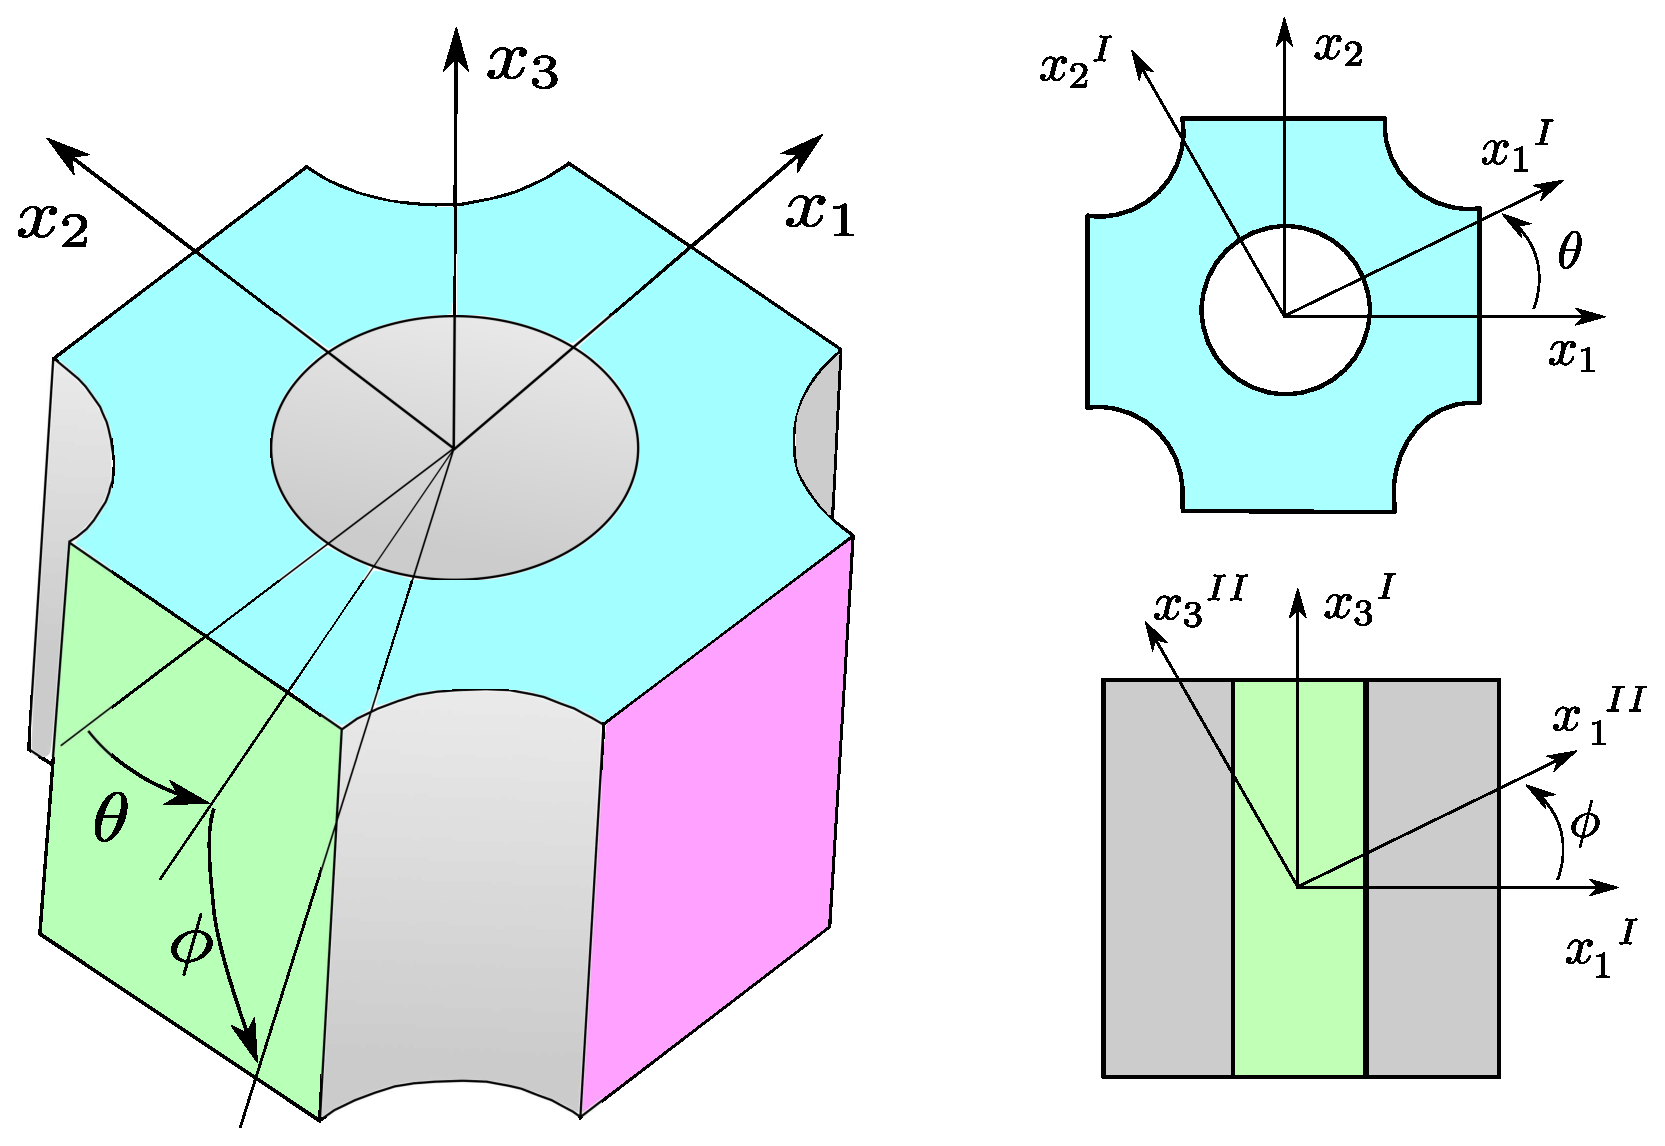
\includegraphics[width=0.8\linewidth]{chapter_4/figure/cell_3d}
	\caption{REV for the fiber geometry investigated.}
	\label{fig:cell_3d}
\end{figure}


%%%%%%%%%%%%%%%%%%%%%%%%%%%%

\subsection{Numerical setup}
\label{ph:numeric_setup}

%%%%%%%%%%%%%%%%%%%%%%%%%%%%


The simulations have been carried out with the open-source code OpenFOAM \citet{openfoam}, based on  a finite volume discretization with a staggered arrangement for the unknowns.
The standard solver icoFoam (incompressible Navier-Stokes) has been modified in order to include a constant pressure gradient acting as a forcing term $\mathbf{f}$  in equation \eqref{eq:ns_f}. 
The coupling between  the velocity and the pressure equations is based on the pressure implicit split operator referred to as the PISO algorithm. 
The time derivative term is discretized using the second order backward Euler scheme and all the spatial terms use a second-order central difference stencil  based on Gauss finite volume approach. The velocity system is solved with a preconditioned bi-conjugate gradient (PBiCG) iterative solver with the tolerance on the velocity residuals set to $10^{-8}$, associated to a   diagonal incomplete lower upper pre-conditioner (DILU).
The pressure equation is solved with a geometric-algebraic multigrid (GAMG) algorithm associated to a Gauss-Seidel smoother and the tolerance on the pressure residuals is here equal to $10^{-6}$.  Cyclic boundary conditions are applied to all fields on all fluid
boundaries along the three directions, and the no-slip condition is imposed on the surface of the solid inclusions. 
The time step $\Delta t$  is automatically determined to ensure  that the maximum Courant number, $Co$, respects the condition:
$Co =  ||v_\beta||  \ \Delta t / \Delta x < 1/2 $, in which $||v_\beta||$ is the local velocity magnitude in the REV and $\Delta x$ is the local grid spacing. $Co$ 
is basically the ratio between the fluid speed  and the velocity to propagate information through the mesh and the condition $Co < 1/2$ is found to be sufficient to have a stable solver.



%%%%%%%%%%%%%%%%%%%%%%%%%%%%%%%%%%%%%%%%

\subsection{Mesh convergence analysis }

%%%%%%%%%%%%%%%%%%%%%%%%%%%%%%%%%%%%%%%%


The mesh has been computed using  the internal OpenFOAM mesher named \textit{snappyHexMesh}.
The final grid is mainly composed by hexahedral cells with a refined regular grid in the boundary layer regions next to the solid surfaces.
Three different mesh sizes, with $0.65 \times 10^6$, $10^6$ and $1.5 \times 10^6$ elements, have been tested in order to demonstrate spatial convergence. This has been assessed using the Grid Convergence Index ($GCI$) introduced by \citet{roache}.

Details of the coarsest mesh used are shown in figure \ref{fig:mesh1}. On the  right frame a close up of the grid in the neighbourhood of the fiber's boundary is displayed: twenty points are used in the structured portion of the mesh along the wall-normal direction.

\begin{figure}[h]
	\centering
	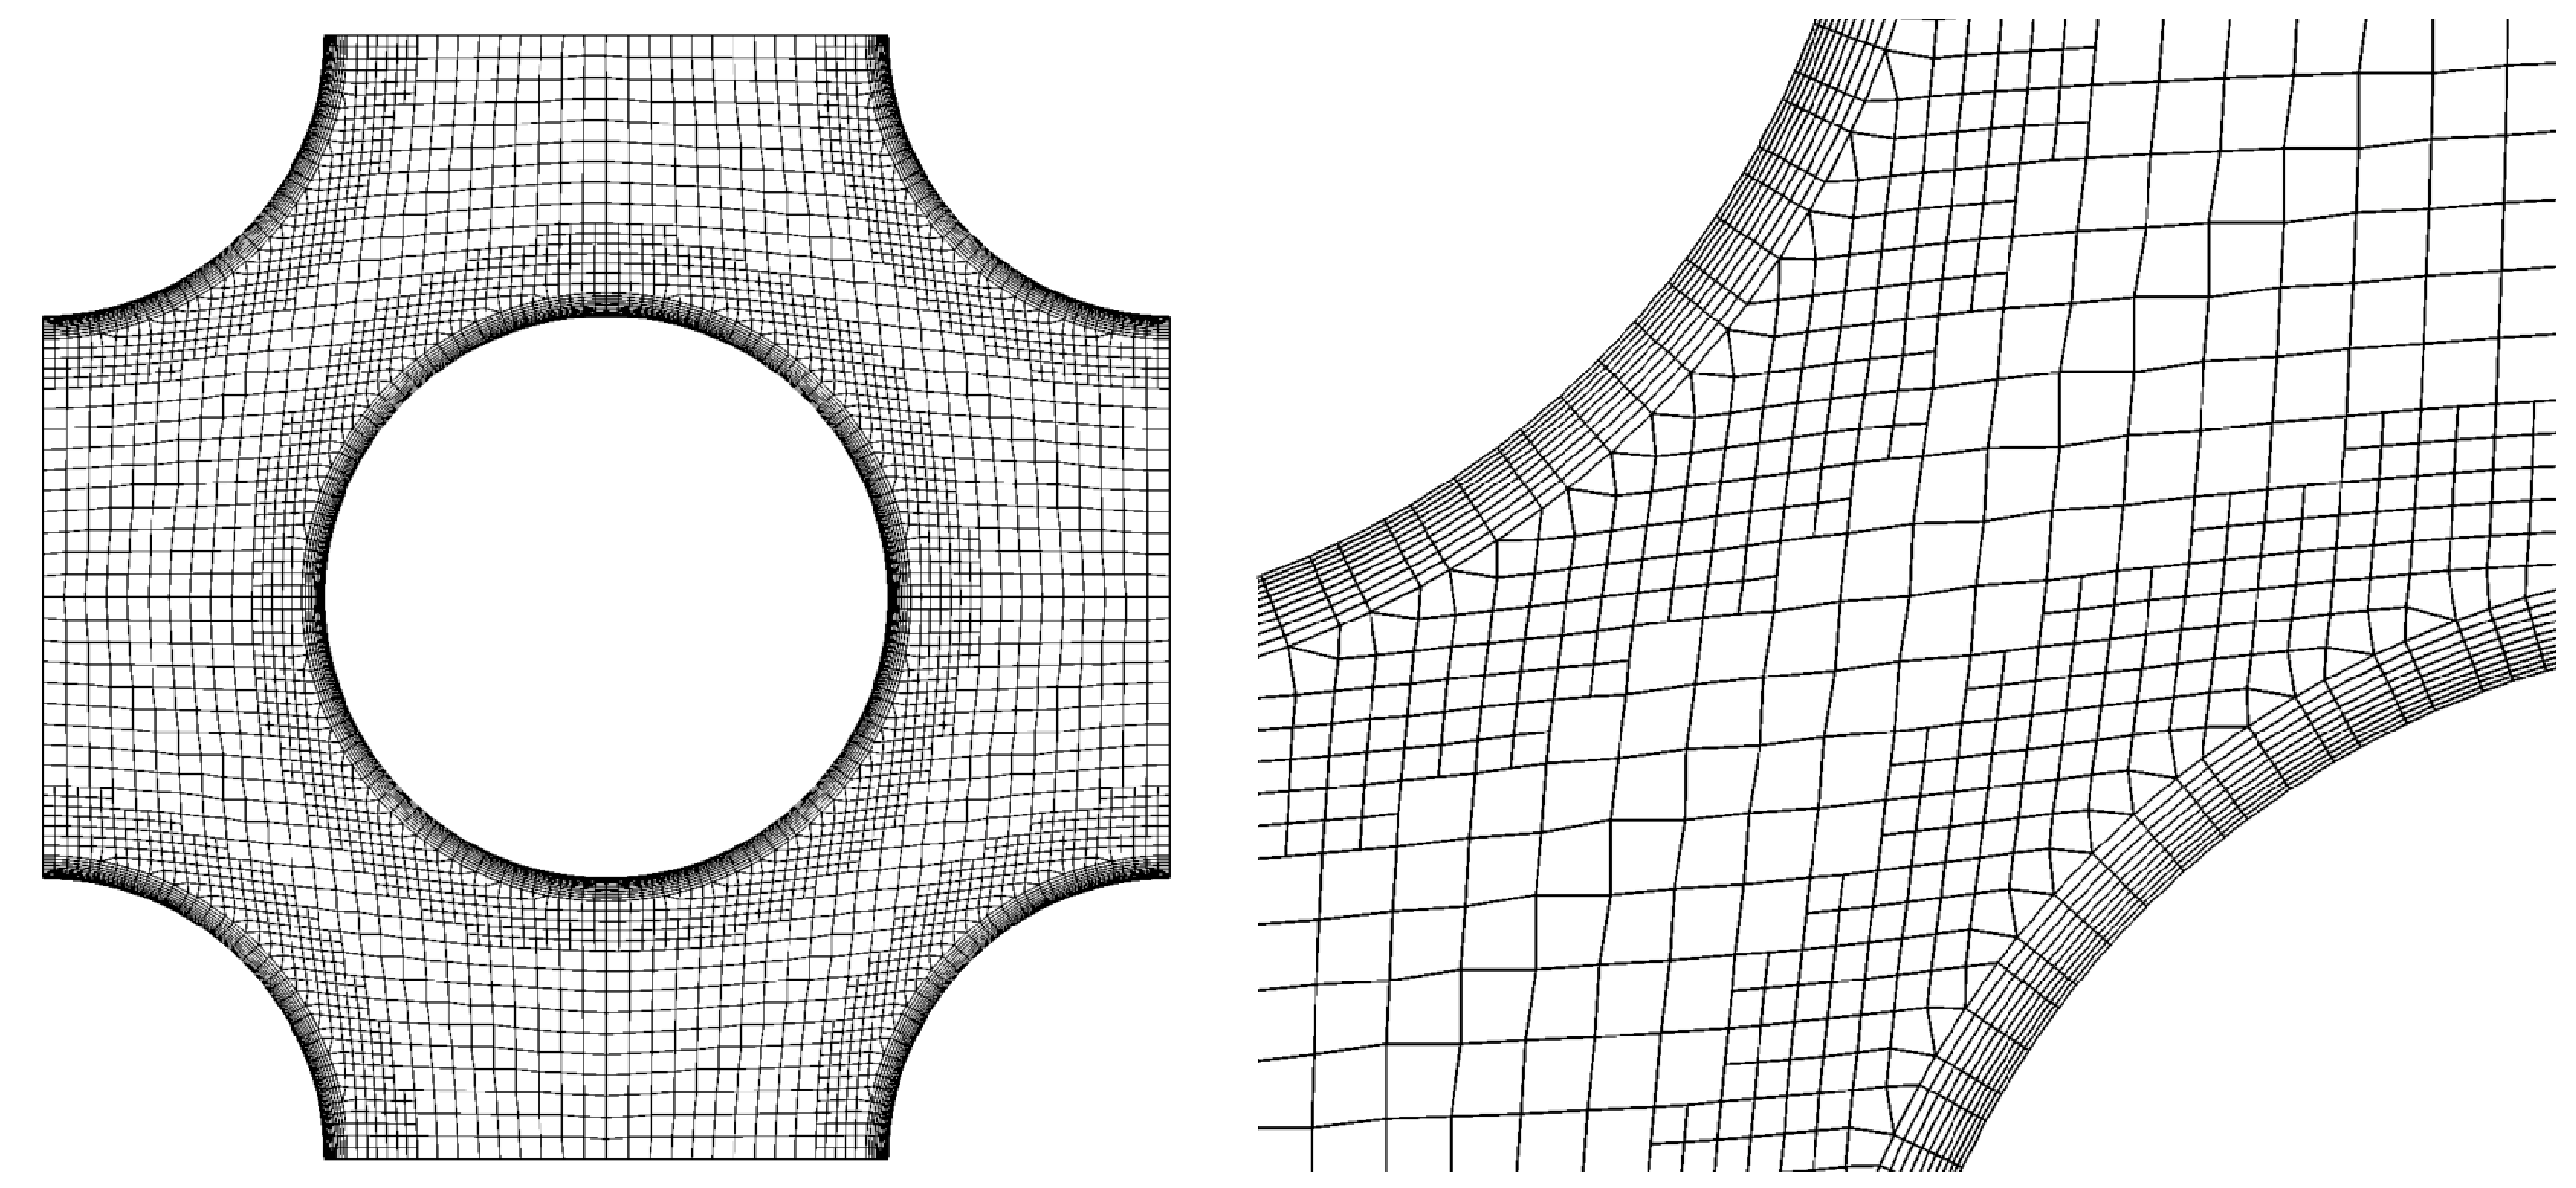
\includegraphics[width=0.8\linewidth]{chapter_4/figure/mesh}
	\caption{Mesh used for the computation; top view (left) and zoom in the boundary layer region (right). $\varepsilon = 0.6$.}
	\label{fig:mesh1}
\end{figure}

The GCI method is based upon a grid refinement error estimator derived from the
theory of generalized Richardson extrapolation. It measures the ratio between the computed value of a quantity over the asymptotic numerical value, thus indicating how far the solution is from the asymptotic ("exact") value.
The procedure is simple and provides a method to estimate the order of the spatial
convergence, based on two or three different grid sizes.
First of all, the grids must be generated with the same algorithm and they must  have the same final quality.
In each simulation  a physical scalar quantity representative of the physical phenomenon must be sampled.
The method follows the following four steps:

\begin{enumerate}
	\item  Estimate the order of convergence of the procedure, defined as
	$p = \ln \rprth{\dfrac{f_3 - f_2}{f_2 - f_1}}   / \ln r $,
	where $r$ is the grid refinement ratio between each grid (it is computed as the ratio between the number of elements of two consecutive grids; the approach imposes that $r$ should remain constant between any couple of consecutive grids and be larger than $1.1$), and $f_i$
	represents the quantity of interest in each grid (1=coarse, 2=medium and
	3=fine).
	
	\item Compute the relative error between grid $i$ and $j$:
	${|\epsilon|}_{ij} = \dfrac{f_j - f_i}{f_i}$, for $(i,j)$
	$\in \left\{ (1,2), (2,3) \right\}$.
	
	\item Compute
	$ {GCI}_{ij}=\dfrac{F_s {|\epsilon|}_{ij}}{r^p -1}$, with
	$F_s$ a safety factor equal to 1.25 if the grids are three, and equal to 3 if the grids are only two \citet{roache}.
	
	\item Check whether each grid level yields a solution that is in the asymptotic range of convergence; this means that the quotient
	$ AC = \dfrac{{GCI}_{23}}{{GCI}_{12}} \dfrac{1}{r^p}$ should be as close as possible to one.
\end{enumerate}


\noindent In our case the quantity of interest chosen is the intrinsic average velocity inside the porous medium, and the results are summarized in table \ref{table:convergence}.
\begin{table}[t]
	\begin{center}
		\begin{tabular}{ l  |l   l   }
			%\vspace{0.1cm}
			mesh   &	mesh   & average REV  \\
			index  &	identifier  &  velocity \\ 
			\hline \hline
			3 &	fine & 1.11  \\ 
			2 &	medium & 1.07  \\ 
			1 & coarse & 1.09  \\ 
			\hline
		\end{tabular}
		$\qquad$
		\begin{tabular}{ l | l } %\vspace{0.35cm} 
			metric & value \\ \hline \hline
			${GCI}_{23}$ & 0.366\%  \\ 
			${GCI}_{12}$ & 1.11\%  \\ 
			AC & 1.006  \\
			\hline
		\end{tabular}
		\caption{Convergence analysis. Left: average velocity within the REV, normalized with $\displaystyle{\frac{K_{11}}{\nu_{\beta}} ||\bf{f}||}$. 
			Right: grid convergence metrics. The REV has $\varepsilon=0.6$, the motion is along $x_1$, i.e. 
			$\theta=\phi=0$ and $Re_d \rightarrow 0$.}
		\label{table:convergence}
	\end{center}
\end{table}
From the table it can be seen that the intrinsic velocity difference is very small from one grid to the next and the coarse grid provides results close to the expected asymptotic value. This is taken as a sufficiently convincing argument to carry out all the computations in the following with a grid density equal to that of grid 1. 



%%%%%%%%%%%%%%%%%%%%%%%%%%%%%%%%%%%%%%%%%%%%%%%%%%%%%%%
\subsection{Validation on two different configurations}
%%%%%%%%%%%%%%%%%%%%%%%%%%%%%%%%%%%%%%%%%%%%%%%%%%%%%%

The results published in the literature by \citet{zampogna2016fluid} and \citet{yazdchi2011} are now used to validate both the methodology and our choices of the computational parameters. In the cited papers, three-dimensional  computations of the permeability components in different cells geometries are presented.

Figure \ref{fig:square} displays the comparison for a cell with a square arrangements  of the fibers; here the permeability is evaluated along the two principal directions, $x_1$ and $x_3$.
%The present computation are plot with triangles for the two $K_{11}$ and $K_{33}$ components.
A good agreement is found with the published results. 
%For permeability $\varepsilon$ larger than $0.85$, some small discrepancies can be seen but it is at the limit of the theory.
%The trends are well captured as well by comparison with the empirical fitted solution given by the reference.
\begin{figure}[t]
	\centering
	\includegraphics[width=0.8\linewidth]{chapter_4/figure/square}
	\caption{Permeability versus porosity for a square arrangement of cylinders. The scaling of the permeability is $\ell^2$ and is explicitely indicated in the vertical axis.}
	\label{fig:square}
\end{figure}
Figure \ref{fig:hexa} shows a similar comparison for a staggered arrangement of the inclusions in the unit cell. In this case the section of the cell is rectangular. The agreement for the only permeability component available in the literature is again satisfactory.
\begin{figure}[h]
	\centering
	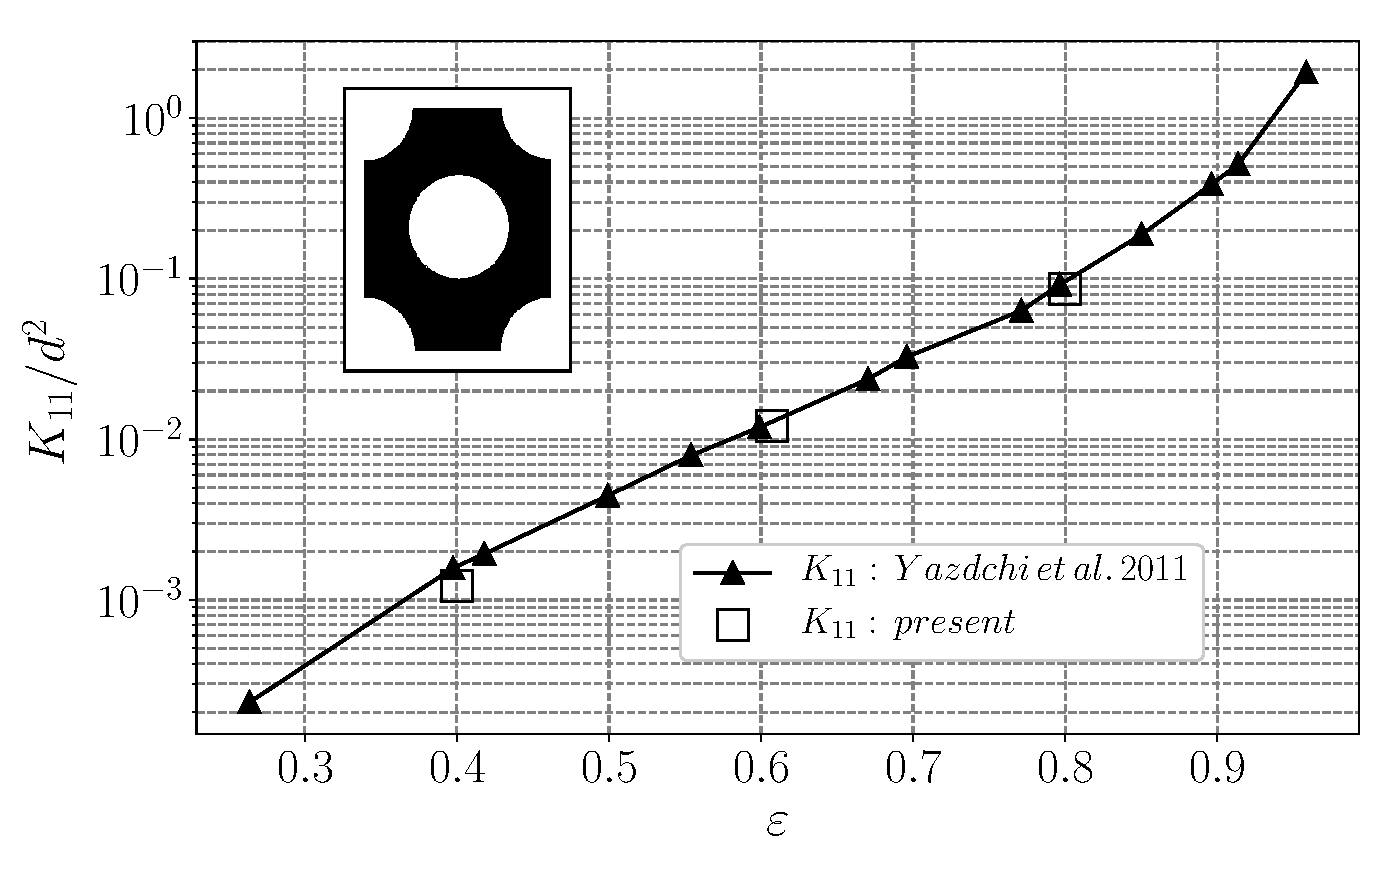
\includegraphics[width=0.8\linewidth]{chapter_4/figure/hexa}
	\caption{Permeability versus porosity for a staggered arrangement of cylinders. The permeability component is here scaled with $d^2$ (and not $\ell^2$), with $d$ the diameter of the inclusions.}
	\label{fig:hexa}
\end{figure}

\begin{figure}[h!]
	\centering
	\includegraphics[width=0.8\linewidth]{chapter_4/figure/macro_force}
	\caption{Relative error between the microscopically computed forces along the $x_1$ direction and those arising from the Darcy-Forcheimmer model; $\varepsilon=0.8$ for the REV in the staggered arrangement of \citet{yazdchi2011}.}
	\label{fig:force_comparison}
\end{figure}	
Finally, to check the correct implementation of the closure model \eqref{eq:closure_model} it is important to verify the equality between the amplitude $F^M$ of the macroscopic force and its microscopic counterpart $F^m$ obtained through an integration of the DNS fields over the solid boundaries of the inclusions in the REV. Figure \ref{fig:force_comparison} shows a plot of the relative error between these two forces, i.e. 
$\displaystyle \frac{||F^M-F^m||}{||F^m||}$, as function of the Reynolds number. We consider the successful comparison displayed in figure \ref{fig:force_comparison} 
as the conclusive demonstration of the validity of the approach described here. We have nonetheless carried out the same verification displayed in figure \ref{fig:force_comparison} for each one of the simulations described in the following, to our satisfaction.



%%%%%%%%%%%%%%%%%%%%%%%%%%%%%%%%%%%%%%%
\subsection{Tests with larger REV's}
%%%%%%%%%%%%%%%%%%%%%%%%%%%%%%%%%%%%%%%

Since the Reference Elementary Volume (REV) is the unit cell within the porous medium over which average quantities of the VANS are computed, 
it is important to choose its dimensions appropriately in the inertial regime for, if the REV is too small, it might be easy to miss crucial 
features of the wakes. For example, to predict the  critical Reynolds number, $Re_c$, of the first Hopf bifurcation, a REV containing at least 
three solid inclusions in the direction of the mean pressure gradient is necessary in the simulations by \citet{lasseux_hopf}. Among the 
results 
reported, it is found that, for a fixed REV size, the error committed in the evaluation of the critical Reynolds number increases with the 
porosity. This same error is considerably reduced when the mean pressure gradient angle is $\theta=45^\circ$. Thus, the choice of the number of 
inclusions in a REV is a task not to be overlooked, and the final choice must account for the porosity, the direction of the pressure gradient 
and the microscopic Reynolds number.

Here, the influence of the numbers of inclusions present in a REV is assessed by focussing only on the velocity components after averaging over the REV. The unit cubic cell of side $\ell$ is used as reference: starting from this, two additional REV's are built, as shown in figure \ref{fig:multiple}. The first one is doubled in both the $x_1$ and $x_2$ directions and the case tested numerically is characterised by $\theta=0$, $\phi=0$ (i.e. the forcing pressure gradient is directed along $x_1$), porosity $\varepsilon=0.6$ and $Re_d=50$. 
The second REV configuration is a composition of 3 reference REVs on top of one another along $x_3$, with the parameters set to $\theta=45^\circ$, $\phi=45^\circ$,  $\varepsilon=0.6$ and $Re_d=100$.

For both these test cases, no appreciable differences, neither in the mean velocity nor in the forces on the fibers, have been observed, with relative errors on the mean velocity with respect to the reference case which remain below  2\%.  We take this as sufficient evidence to use, in the following, only the reference cubic REV of side equal to $\ell$, with the understanding that only configurations with $Re_d$ up to around 100 can be considered.

\begin{figure}[h!]
	\centering
	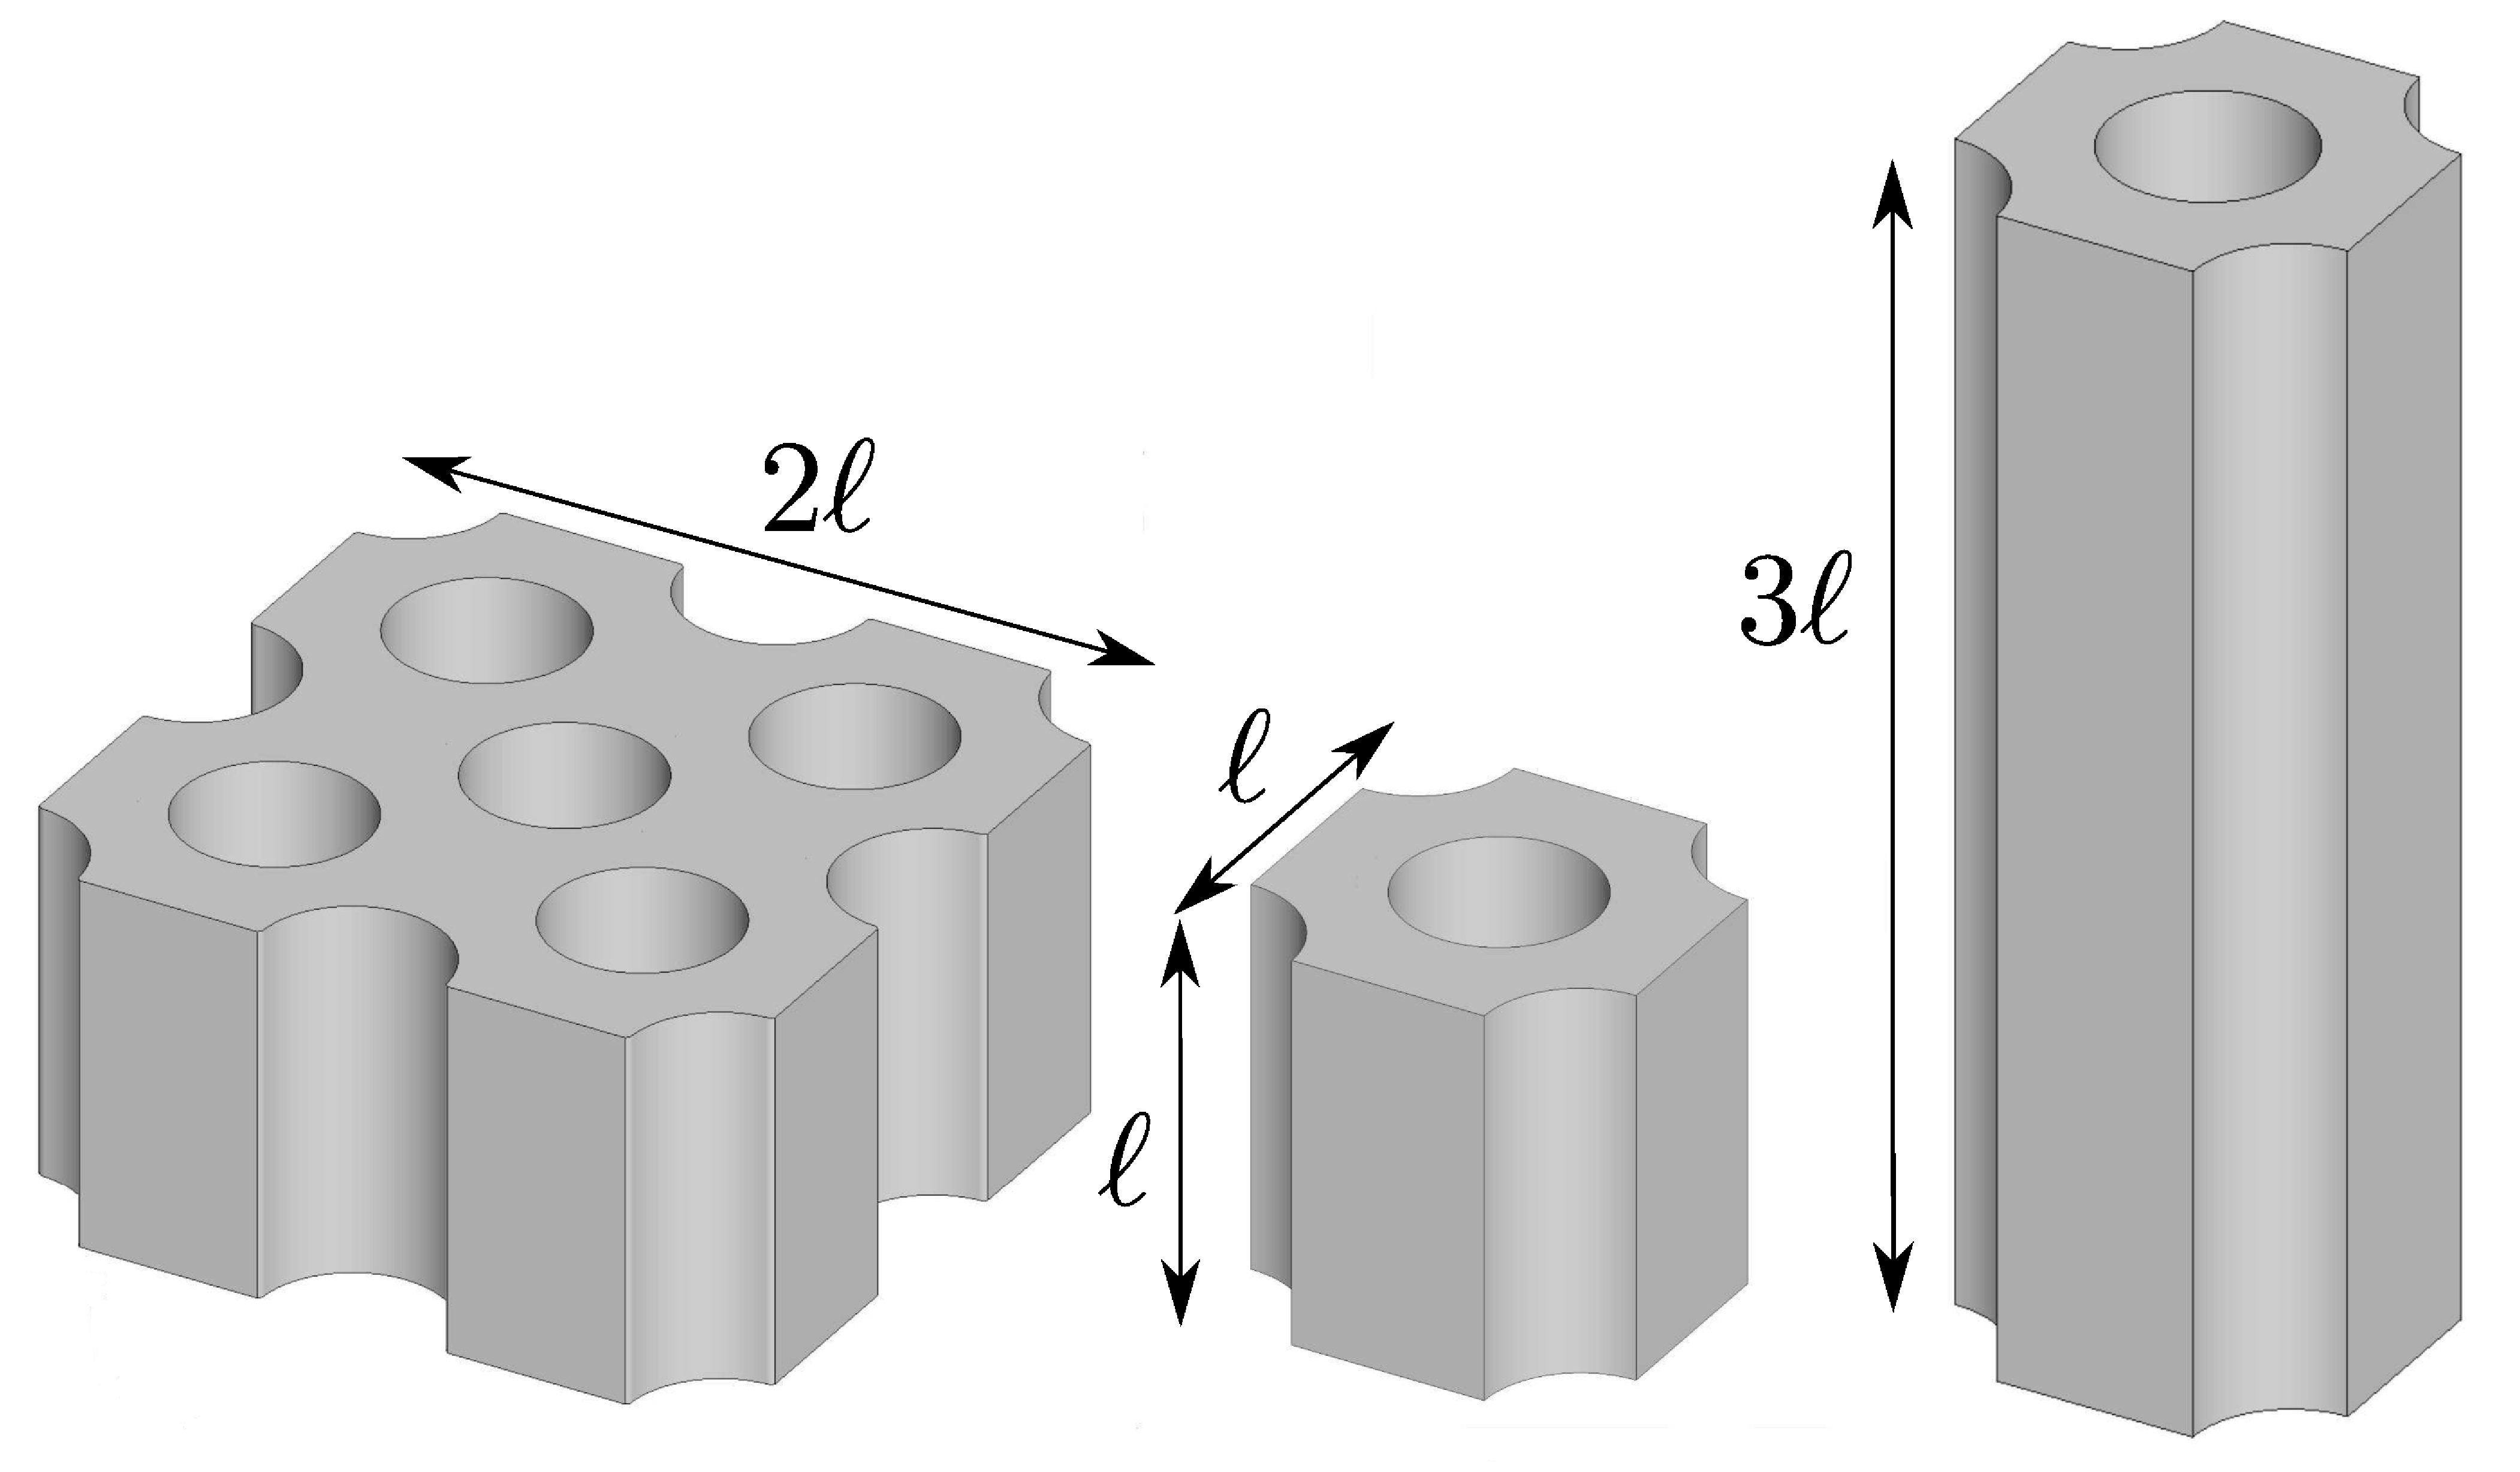
\includegraphics[width=0.8\textwidth]{chapter_4/figure/multiple}
	\caption{REV configurations. Left: $2 \times 2 \times 1$ arrangement; centre: $1 \times 1 \times 1$ arrangement (reference);  right $1 \times 1 \times 3$ arrangement.}
	\label{fig:multiple}
\end{figure}



%%%%%%%%%%%%%%%%%%%%%%%%%%%%%%%%%%%%%%%%%%%%%%%%%%%
\section{Microscopic solutions}
%%%%%%%%%%%%%%%%%%%%%%%%%%%%%%%%%%%%%%%%%%%%%%%%%%

In this section, some local microscopic fields computed with direct numerical simulations are shown, together with components of the intermediate tensor $\mathbf{M}$ coming from the numerical solution of the closure equations \eqref{eq:h_model}. 

In figure \ref{fig:1ch4} (top row) the local $x_1$ velocity component is drawn for the two-dimensional flow when $\varepsilon=0.6$, for three 
Reynolds numbers, to cover the transition from the Stokes to the inertial regime. In all plots, the velocities are rendered non-dimensional by
the corresponding value of 
$\displaystyle{\frac{K_{11}}{\nu_{\beta}} ||\bf{f}||}$. When inertia is absent, the flow has a central symmetry; by increasing the Reynolds number, only the 
symmetry with respect to the $x_1$ axis is maintained ($x_1$ is the direction of the forcing pressure gradient), with the wake's length which 
increases with $Re_d$. When $Re_d$ is of order 100 the wake spreads to the downstream boundary of the REV, re-entering, because of periodicity, 
at the upstream side.	This $Re_d$  represents the upper limit of validity for the cubic unit cell of side $\ell$; larger values of $Re_d$ 
could only be investigated with longer/larger/thicker REV's.

The non-dimensional local $M_{11}$ fields for the same parameters are displayed in figure \ref{fig:1ch4} (mid row). All values in the figures 
arise from scaling $\bf{M}$ with $\ell^2$. Visually, these local fields are strongly correlated to the local streamwise velocity component in the whole $Re_d$ range. 
This is not unexpected since the local velocity drives the convective term of system \eqref{eq:h_model}. 
The central symmetry of all components of $\bf{M}$ in the Stokes regime is coupled to the rotational invariance of the apparent permeability tensor in two-dimensional flows.

The effect of varying the porosity is shown in figure \ref{fig:1ch4} (bottom row) where $\varepsilon$ is taken equal to $0.4$. Even at such a
low porosity the stretching of the wake can be noticed, and it increases with $Re_d$. Interestingly, this effect is milder when
the forcing is inclined by an angle $\phi$, since the tighter packing of the inclusions causes a strong deviation of the mean flow along the axis of the fiber. In this case, $M_{11}$ and $M_ {22}$ behave very similarly to the case $\phi = 90^{\circ}$.    


\begin{figure}[H]
	\centering
	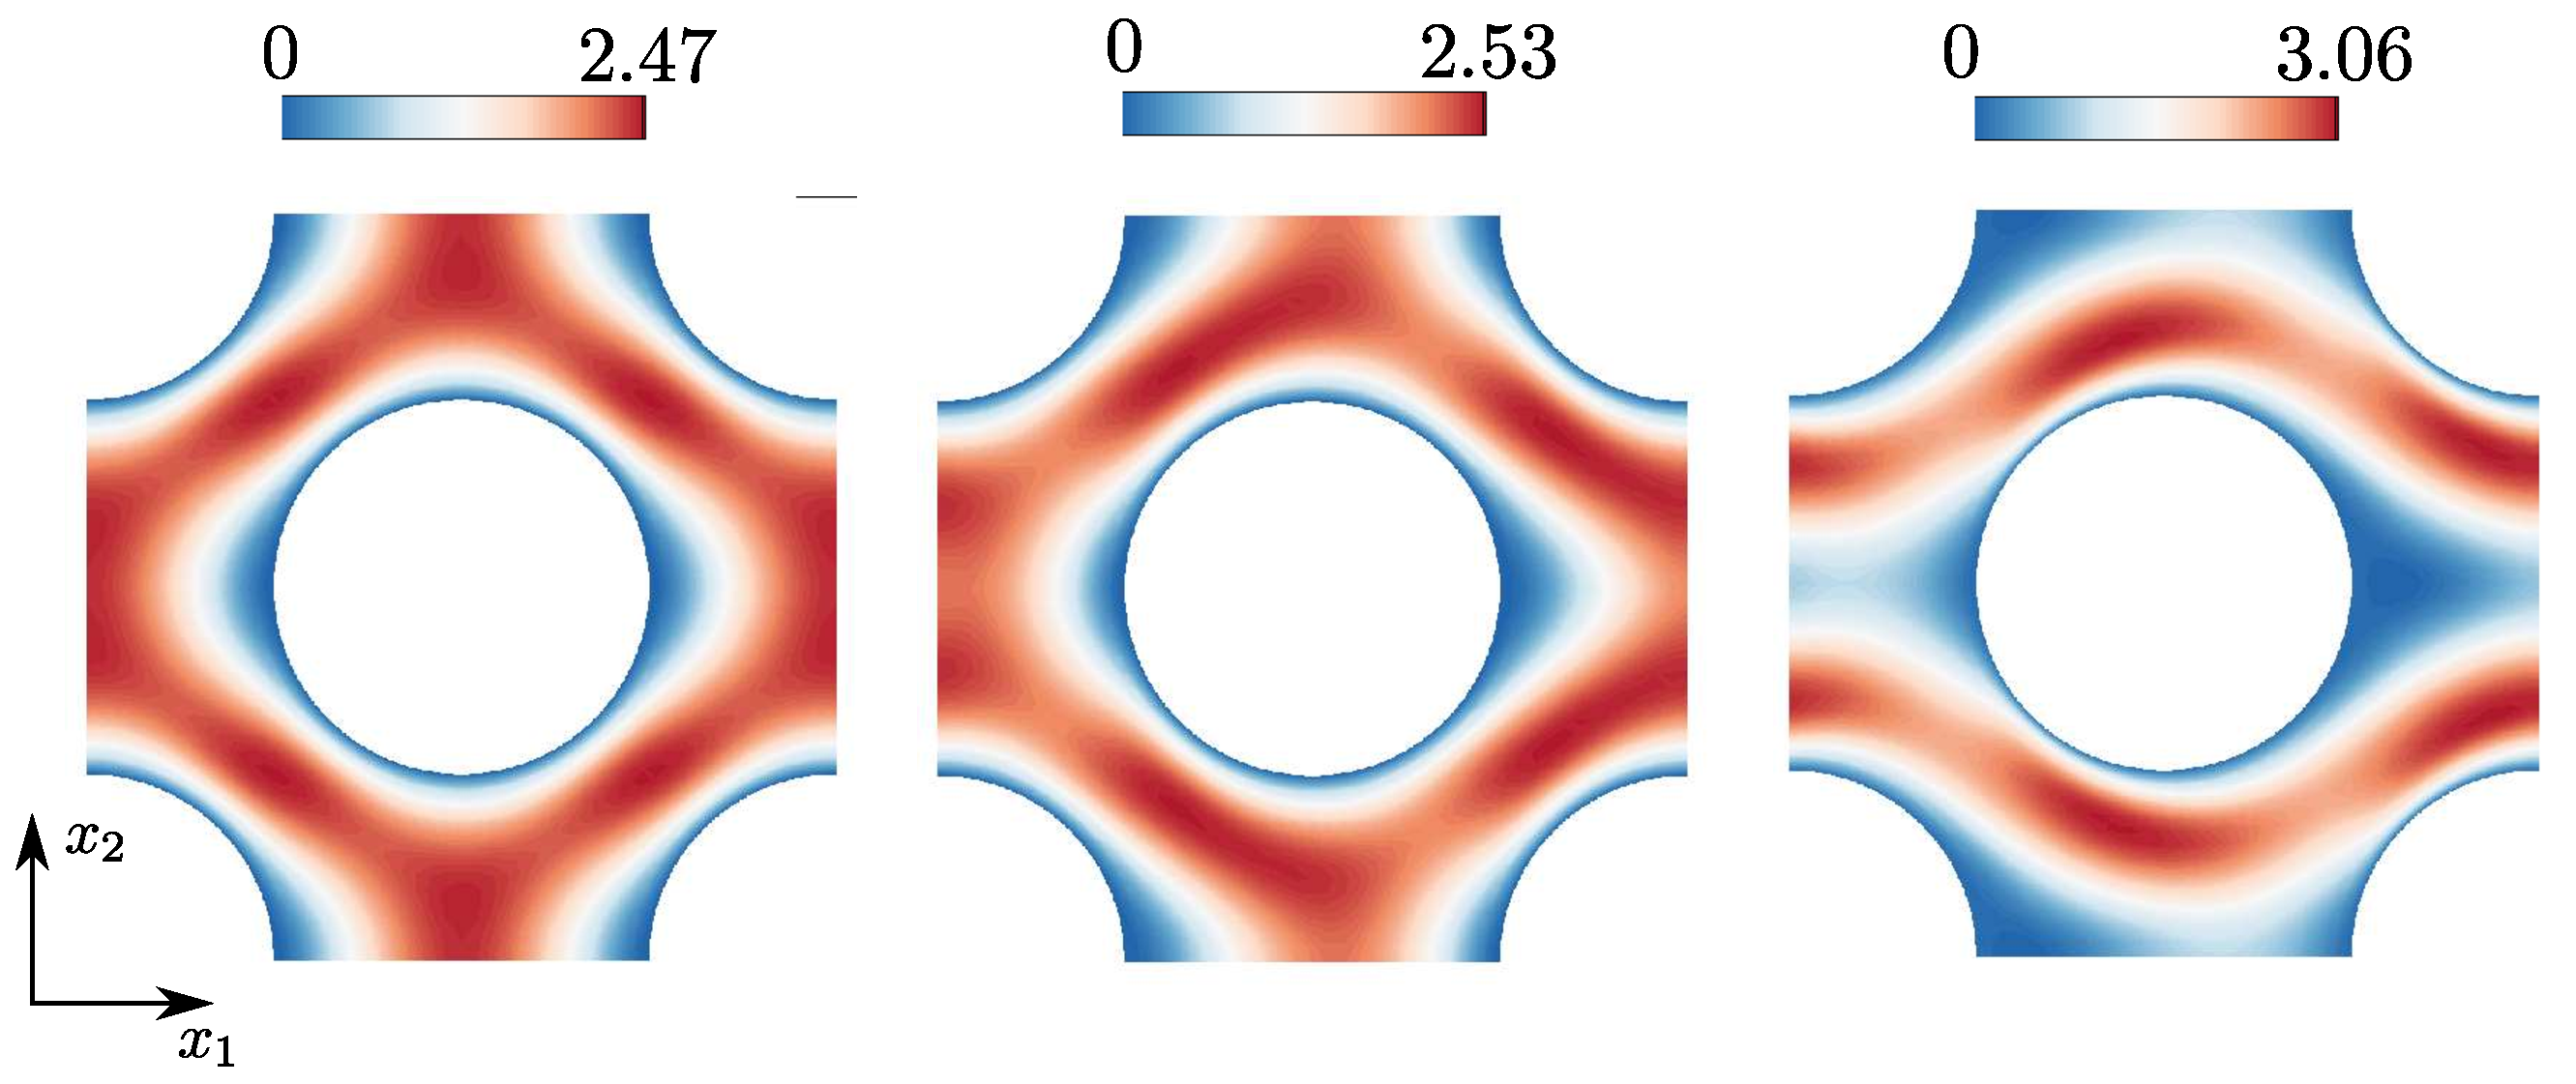
\includegraphics[width=0.85\textwidth]{chapter_4/figure/fig1}
	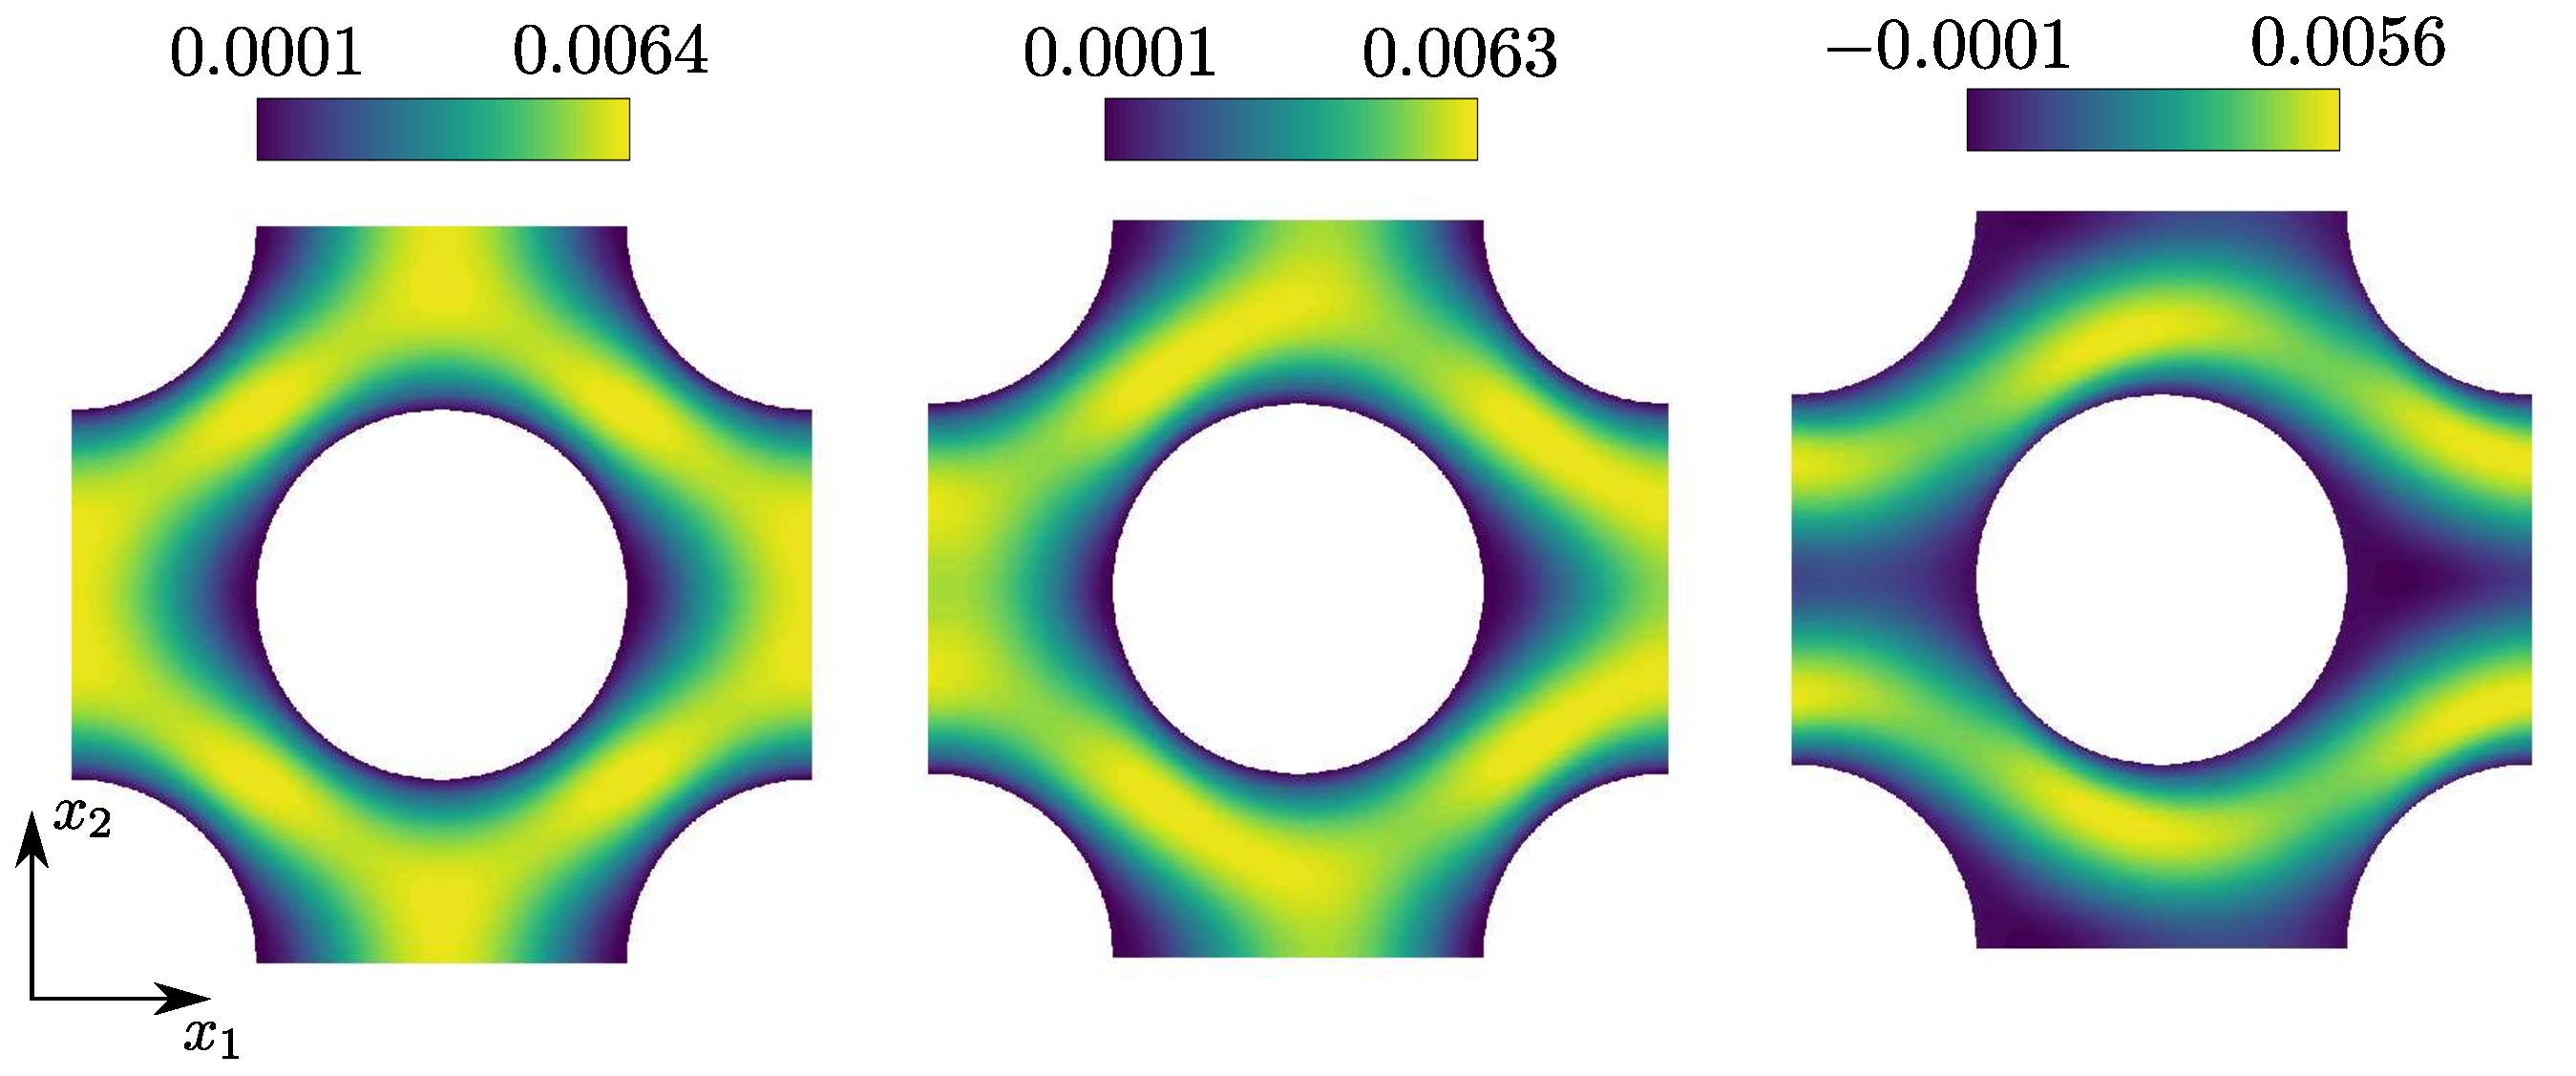
\includegraphics[width=0.85\textwidth]{chapter_4/figure/fig2}
	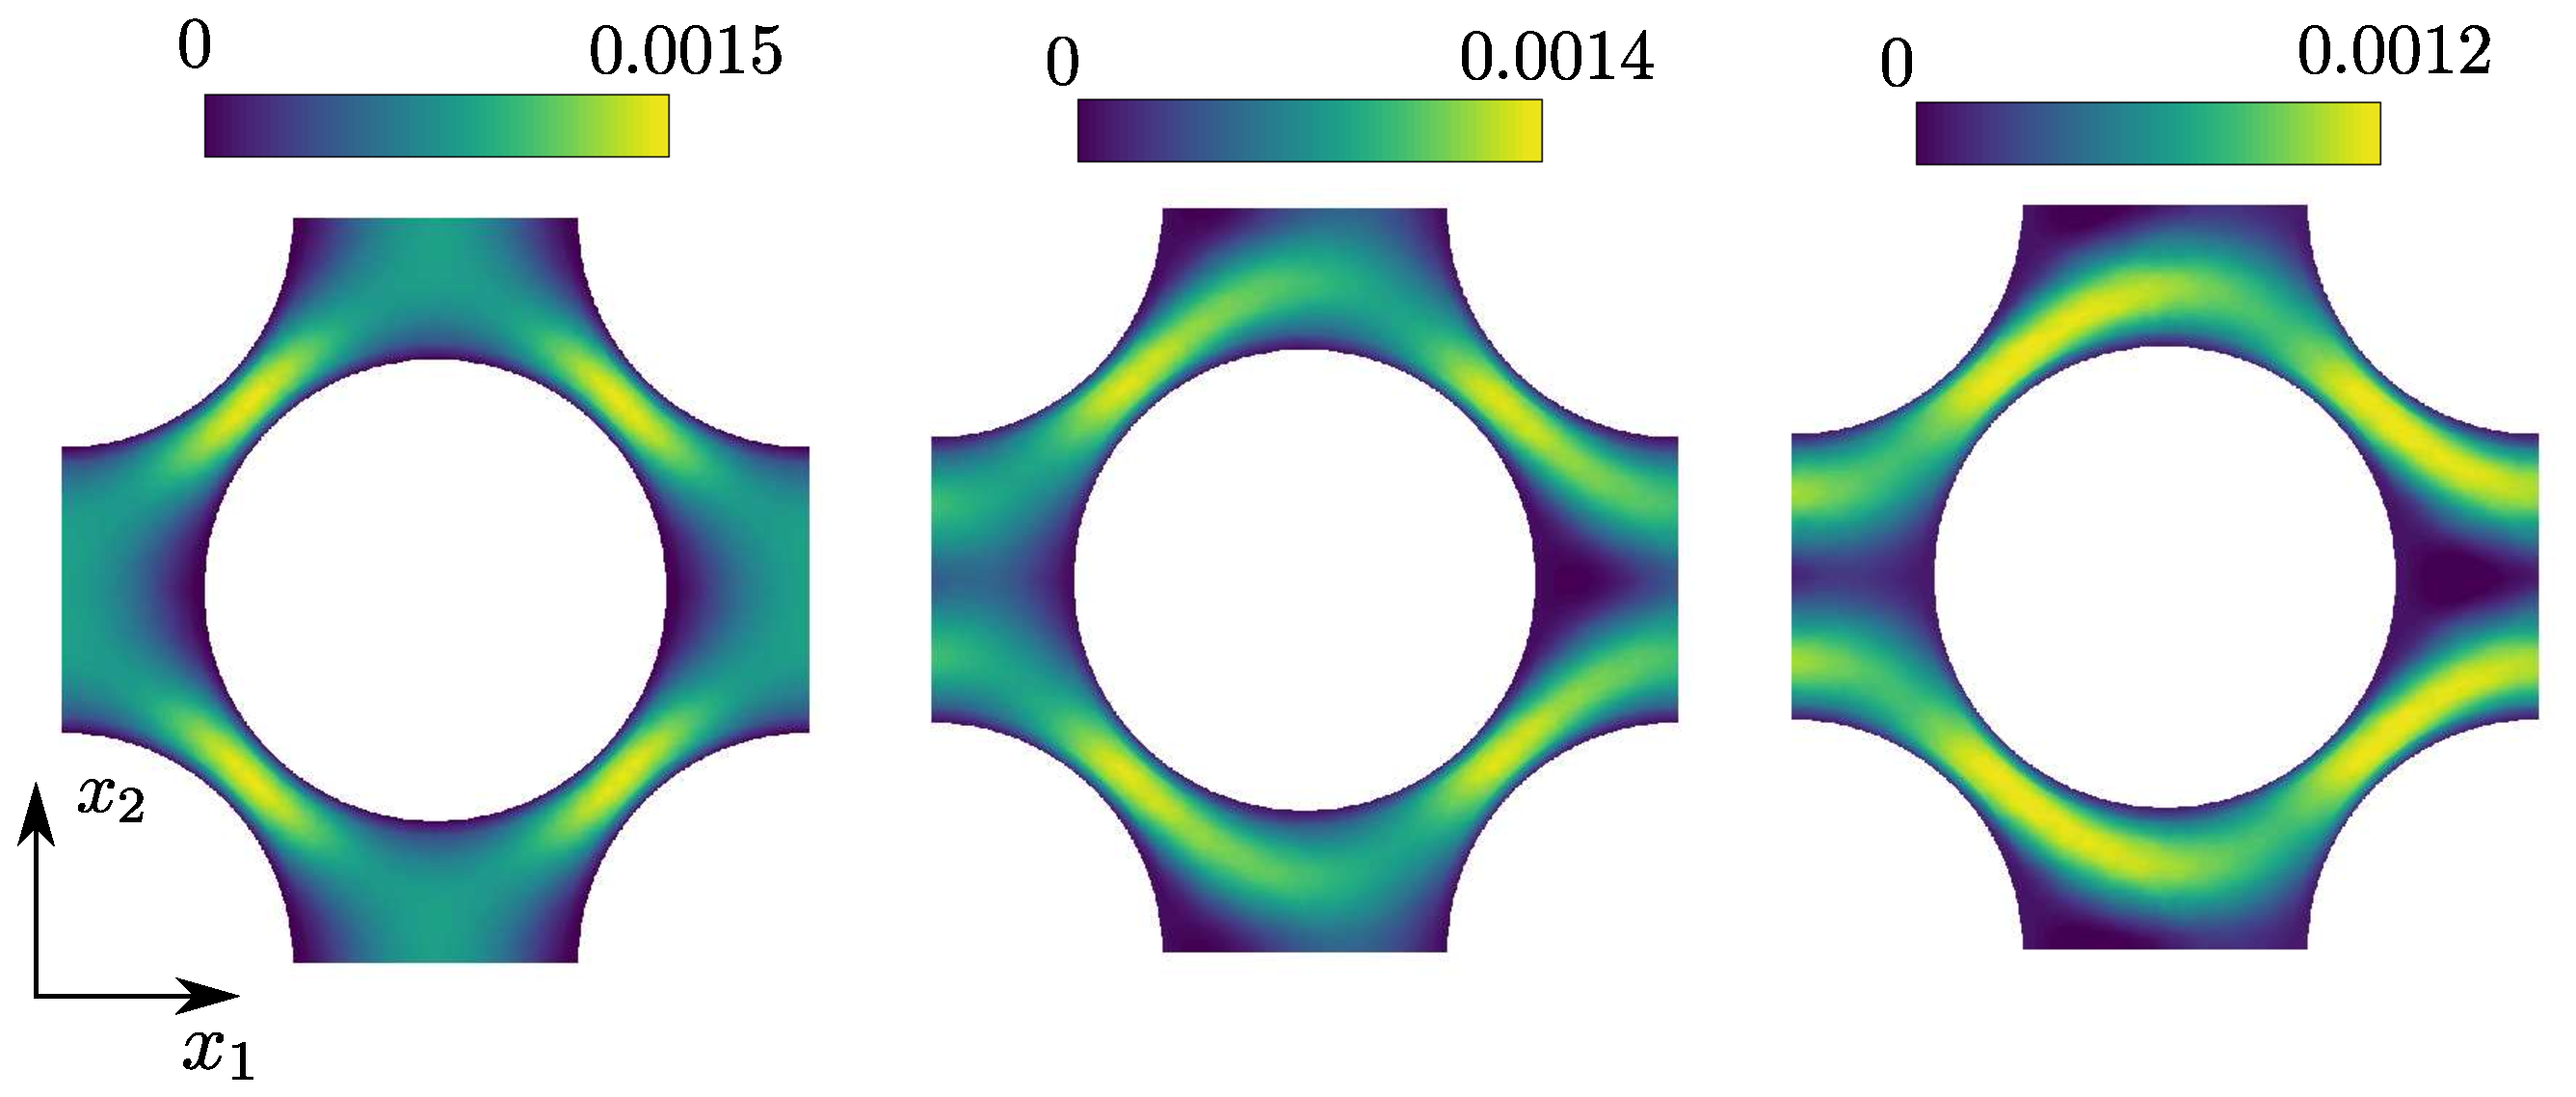
\includegraphics[width=0.85\textwidth]{chapter_4/figure/fig4}
	\caption{Top row: plane view of the dimensionless $x_1$ component of the local velocity field ${\vb}$ for the case $\theta=0,$ $\phi=0$, $\varepsilon=0.6$ and for three Reynolds numbers $Re_d$ = $0,10,50$, from left to right. Mid row: microscopic $M_{11}$ fields corresponding to the images in the top row. Bottom row: $M_{11}$ fields for the same Euler angles and Reynolds number as in the top two rows, and smaller porosity ($\varepsilon=0.4$).}
	\label{fig:1ch4}
\end{figure}


\newpage

Another interesting point emerges by inspection of  figure \ref{fig:3ch4} where two off-diagonal components of $\bf{M}$ are shown for two porosity 
values; the first image (left frame) represents a plane flow in the Stokes regime while the second is the plane cut of a three-dimensional 
solution in the inertial regime. Positive and negative values of the microscopic fields can be seen in both images but, once averaging is 
applied over the REV, the resulting permeability component is very close to zero (in fact, exactly equal to zero in the Stokes case).  This same features occurs for all off-diagonal terms in all cases examined, so that, within the current range of Reynolds numbers, the 
apparent permeability tensor is, to a good approximation, diagonal\footnote{In fact, there are always at least two orders of magnitude 
	differences between the diagonal and the off-diagonal components. While the latter should not, in principle, be ignored, we will focus attention 
	here only on the dominant terms of the permeability tensor.}.


\begin{figure}[H]
	\centering
	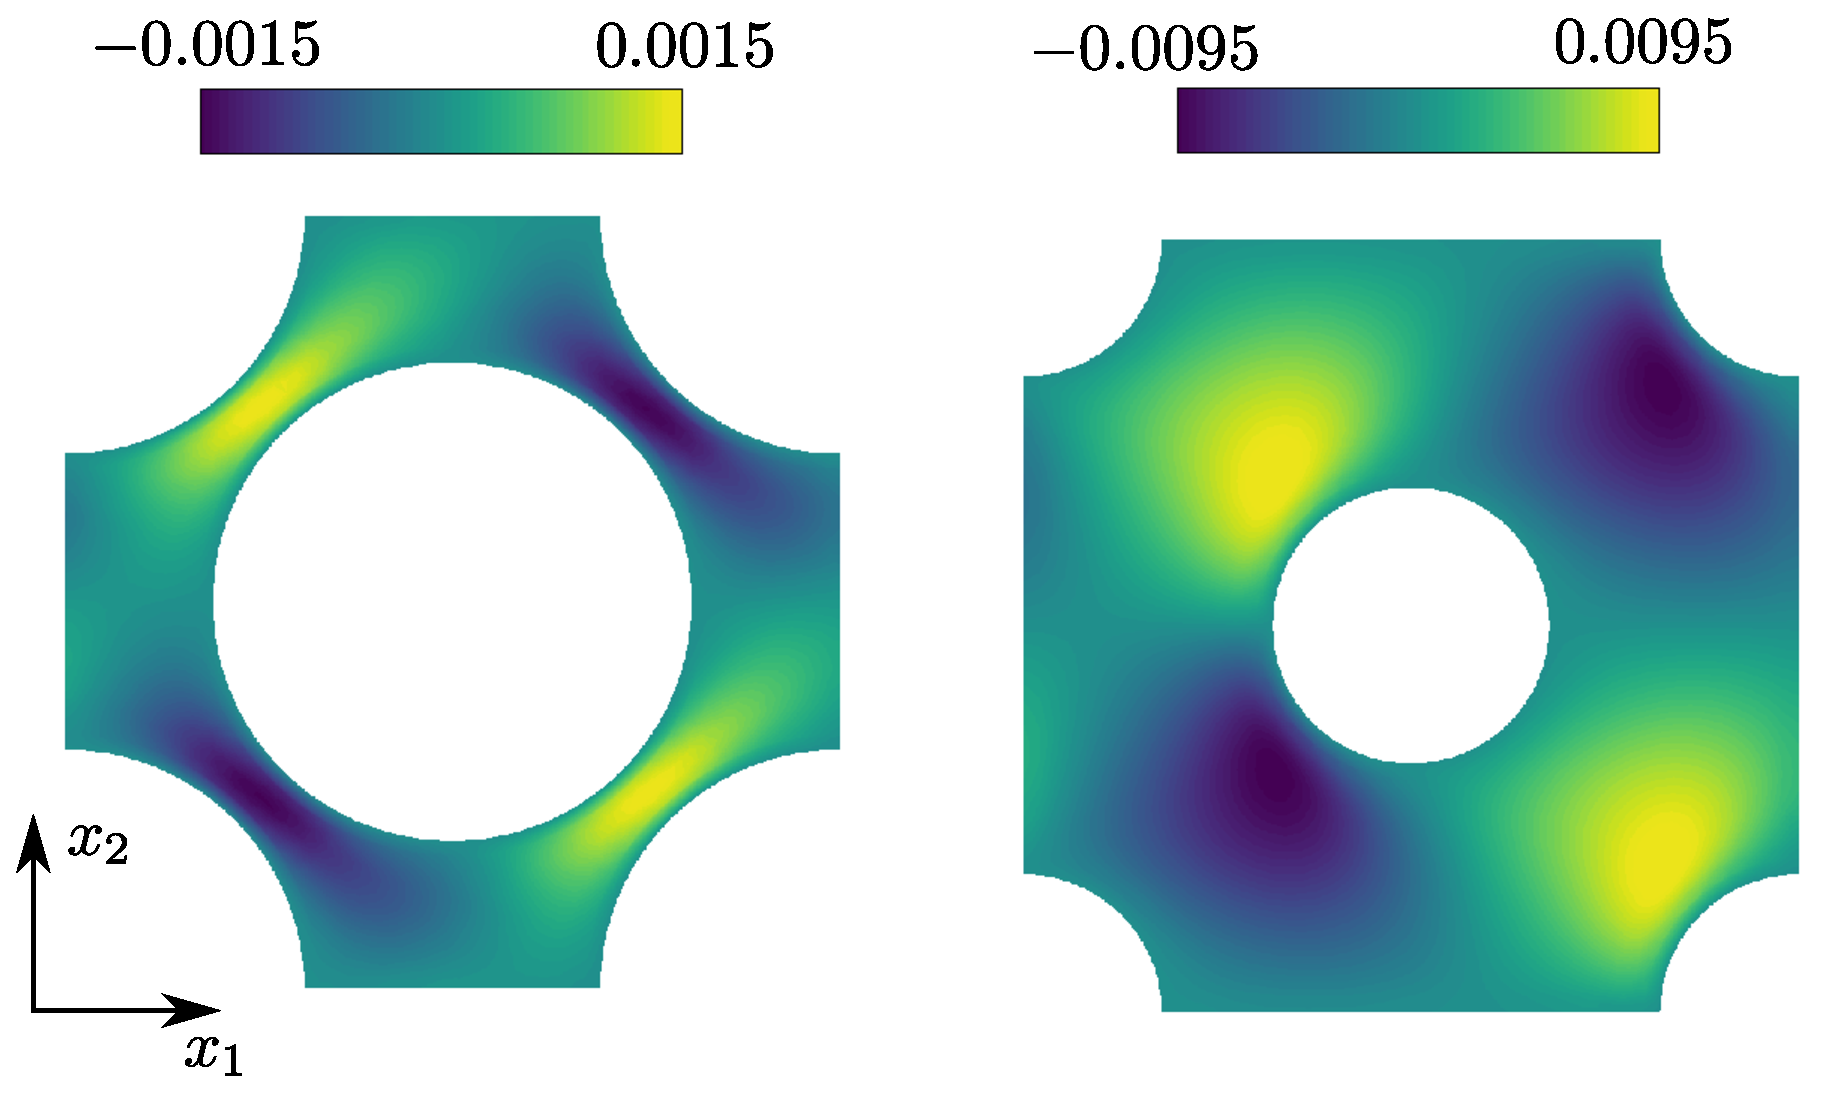
\includegraphics[width=0.8\textwidth]{chapter_4/figure/fig3}
	\caption{right: Non-dimensional $M_{21}$ field for $\theta=0, \phi=0, Re_d=10, \varepsilon=0.8$, left: Non-dimensional $M_{12}$ field for $\theta=22.5^{\circ}, \phi=45^{\circ}, Re_d=50, \varepsilon=0.4$.}
	\label{fig:3ch4}
\end{figure}

A three-dimensional case is shown in  figure \ref{fig:5ch4}, where all the non-zero terms of the $\mathbf{M}$ tensor are plotted for a porous
structure with $\varepsilon=0.6$. The components shown are $M_{11}$, $M_{22}$,$M_{33}$, $M_{12}$ and $M_{21}$, while $M_{i3}$ and $M_{3j}$ are 
not plotted because they are identically zero to machine accuracy. Distinct features are visible in each image; in particular, in the last 
frame the $M_{33}$ microscopic component displays a low wavelength structure along the cylinder's axis. Increasing the dimensions of the REV 
along $x_3$ does not alter such a structure, i.e. the $\ell^3$ domain chosen with its periodic boundary conditions does not filter out 
significant high wave-numbers of the flow. We further note that the tensor $\mathbf{M}$ is not symmetric in this case since each off-diagonal component 
represents the solution of the closure problem in a specific direction (first index of the field) and the forcing term acts orthogonally to it
(second index of the field).  Once averaged over the REV it is found that both $H_{12}$ and $H_{21}$ are very close to zero.  


\begin{figure}[H]
	\centering
	\includegraphics[width=0.6\textwidth]{chapter_4/figure/fig5}
	\caption{Non-dimensional $\mathbf{M}$ components fields for the case $\theta=22.5^{\circ}, \phi=45^{\circ}, Re_d=50, \varepsilon=0.6$.}
	\label{fig:5ch4}
\end{figure}    



%%%%%%%%%%%%%%%%%%%%%%%%%%%%%%%%%%%%%%%%%%%%%%%%%%
\section{The apparent permeability tensor}
%%%%%%%%%%%%%%%%%%%%%%%%%%%%%%%%%%%%%%%%%%%%%%%%%%

\label{sec:5}

In this section the variations of the diagonal components of the permeability tensor $\mathbf{H}$ are discussed as function of the direction of 
the mean forcing, the Reynolds number and  the porosity. As stated previously, the Reynolds number ranges from $0$ to approximately $100$ in 
order to capture phenomena associated with inertia; the cases considered never lead to unsteady signals. 
The porosity parameter $\varepsilon$ is set to either $0.4$ (low porosity),  $0.6$ (medium) or
$0.8$ (high). The forcing direction is defined by the Euler angles and all the configurations considered in this section are summarized in 
table \ref{table:directions}; the choice has been made to explore a reasonably large range of parameters, with both two-dimensional and three-
dimensional flows characterized by symmetric and asymmetric patterns.

Let us briefly recall the methodology. First, a DNS is carried out to compute the microscopic flow. Then the  closure problem is solved for the 
tensor $\mathbf{M}$. Finally, each component of the apparent permeability  $\mathbf{H}$  is obtained by averaging (equation 
\eqref{eq:avg_intrinsic}).
The results are collected in figures \ref{fig:08_H}, \ref{fig:06_H} and \ref{fig:04_H}, showing the variation of the diagonal components 
of $\mathbf{H}$. 


\begin{table}[t]
	\centering
	\begin{tabular}{l | l l l}
		index & $\theta$ & $\phi$ & field properties \\\hline	\hline
		1 & $0^\circ$ & $0^\circ$ & 2D symmetric \\
		2 & $22.5^\circ$ & $0^\circ$ & 2D non-symmetric \\
		3 & $0^\circ$ & $45^\circ$ & 3D symmetric \\
		4 & $22.5^\circ$ & $45^\circ$ & 3D non-symmetric \\
		5 & $-$ & $90^\circ$ & 3D symmetric \\
		\hline  
	\end{tabular}
	\caption{Directions of the forcing tested and property of the solutions.}
	\label{table:directions}
\end{table}



\begin{figure}[H]
	\centering
	\includegraphics[width=1\textwidth]{chapter_4/figure/H_of08}
	\caption{Diagonal elements of the apparent permeability $\mathbf{H}$ as function of the Reynolds number for porosity  $\varepsilon=0.8$. The forcing  direction is represented through the couple of Euler  angles 
		$(\theta,\phi)$ (cf. table \ref{table:directions} for the case index). Left column: low-$Re_d$ regime; right column: inertial regime.}
	\label{fig:08_H}
\end{figure} 

\begin{figure}[H]
	\centering
	\includegraphics[width=1\textwidth]{chapter_4/figure/H_of06}
	\caption{Same as figure \ref{fig:08_H} with porosity $\varepsilon=0.6$.}
	\label{fig:06_H}
\end{figure}



\begin{figure}[H]
	\centering
	\includegraphics[width=1\textwidth]{chapter_4/figure/H_of04}
	\caption{Same as figure \ref{fig:08_H} with porosity $\varepsilon=0.4$.}
	\label{fig:04_H}
\end{figure}

%\begin{figure}[H]
%   \centering
%   \input{figure/H_of04.pdf_tex}
%   \caption{Same as figure \ref{fig:08_H} with porosity $\varepsilon=0.4$.}
%   %\label{fig:04_H}
%\end{figure}
%



In the left column of each figure we focus on the low-$Re_d$ regime ($0 < Re_d < 2$), while in the right column the effect of inertia can be 
assessed.  As expected, when $Re_d$ is small the apparent permeability is quasi-Reynolds-number-independent (and can be approximated well by 
the true permeability). As the Reynolds number increases above a few units, inertial effects grow in importance yielding typically a monotonic decrease of all 
components of $\mathbf{H}$, aside from case indexed 5 ($\phi=90^{\circ}$) for which the flow remains aligned with the cylinder's axis. In case 5 the 
microscopic flow solution is invariant with $x_3$ and does not change with $Re_d$ in the range considered, so that $\mathbf{H}$ is a  
constant tensor.

When the porosity is large all components show a similar behaviour irrespective of the forcing angle (except, clearly, case 5). Differences 
start appearing at $\varepsilon=0.6$; the two cases with $\phi=0^{\circ}$ (index 1 and 2) behave similarly, and so do the two cases indexed 3 
and 4 (with $\phi=45^{\circ}$). This seems to suggest a weaker effect of $\theta$ on the permeability components.  For even smaller porosity ($
\varepsilon=0.4$), the blockage which the inclusions cause to the flow produces the unexpected behaviour displayed in figure \ref{fig:04_H}. 
When the flow is purely two-dimensional (cases 1 and 2), variations in the Reynolds number affect $\mathbf{H}$ significantly; when a pressure 
gradient along $x_3$ is present the strong packing of the fibers constrain the fluid to flow prevalently along the fibers' axis, and the 
apparent permeability is almost $Re_d$-independent. When assessing variations in $H_{jj}$ for this case, attention should also be paid to the 
fact that the permeability is now at least one order of magnitude smaller than in the previous cases so that variations of the diagonal 
components shown in figure \ref{fig:04_H} are tiny in absolute terms.  This is related to the fact that  the  inverse of the permeability  
plays the role of a drag coefficient in the macroscopic expression of the force  (cf. equation \eqref{eq:vans_mom_1}).  In other words, 
materials with higher porosity (larger space between solid inclusions) offer lower resistance to the motion of the fluid.


%In the simulations carried out the off-diagonal terms are consistently at least two orders of magnitude smaller than their diagonal 
%counterparts, for all parameters considered.  
Applying the intrinsic average operator to the non-diagonal component of the tensor $\mathbf{M}$ results in terms that are negligible with respect to their diagonal counterparts, and these results are true for all the parameters considered. This means that there is a very weak coupling between the principal directions of the fiber.
The directional decoupling and the diagonal property of the apparent permeability tensor has also been computationally demonstrated
on a completely different REV geometry by \citet{soulaine2014}. Conversely,
\citet{lasseux} have carried out a two-dimensional study with fibers of square cross-section, finding that the off-diagonal terms are 
non-negligible and only about
one order of magnitude smaller than the diagonal components. This result is a consequence of the non-rotationally-invariant  geometry  
considered.  The present work and the two articles just cited suggest that the  diagonal property of the tensor $\mathbf{H}$   is closely
related to the geometry of the porous material, more  than to the flow regime.  



%%%%%%%%%%%%%%%%%%%%%%%%%%%%%%%%%%%%%%%%%%%%%%%%%%%%%%%%%%%
\section{A metamodel for $\bf H$}
%%%%%%%%%%%%%%%%%%%%%%%%%%%%%%%%%%%%%%%%%%%%%%%%%%%%%%%%%%%

The previous sections has shown how the apparent permeability depends on  the two Euler angles, the Reynolds number and the porosity. The space 
of parameters is formidable and the results found so far are not sufficient to treat, for example, cases characterized by multiple inclusions'
sizes and orientations in different regions of the domain, or cases involving a poroelastic medium, with temporally and spatially varying 
porosity, flow direction and local Reynolds number. The complete solution of the closure problem for a single set of parameters takes 
approximately 4 CPU hours on our two-processor Intel(r) IVYBRIDGE 2.8Ghz, each with 10 cores and 64 GB of RAM, so that a complete parametric 
study is, to say the least, unpractical. In view of this, the construction of a metamodel capable to provide a full characterisation of the 
permeability as a function of all parameters is a worthy endeavor. We have tested several surrogate models, before eventually settling on the kriging 
approach \citet{Kleijnen20171} described in the following.



%Usually the homogenization approaches are used to investigate complex problems in which   length scales  of the physical phenomena are much %larger than the REV one (\citet{ugis})  (\citet{prosperetti}). The aim
%is to avoid to resolve the  length scales smaller the unity (with respect to the REV length) and in consequence to drastically reduce  the %number of mesh cells and the computational load.
%Here the physics at the REV scale is modelled with the VANS method and in particular by identifying the local apparent permeability $%\mathbf{H}$ tensor.

%In addition, it has been shown that the non constant tensor $\mathbf{H}$ required to be evaluated locally and at each time step  in a full %temporal simulation over a large domain with large REV numbers. 
%Especially, at at least the local Reynolds number and the flow direction change from cell to cell, where each cell could be composed of one or %several REV.

%Solving the $\mathbf{H}$ closure problem for a given set of parameters takes approximately 4 hours with our resources [two processor Intel(r) %IVYBRIDGE 2,8Ghz each with 10 cores and 64 GB of RAM], so reiterate the procedure inside each time step for each cell is at least unpractical. 
%
%To circumvent such a problem  the design of a reduce order model, or the use of a metal-model can be a convenient approach.  
%In this work, several metamodel have been investigated and only one is presented in the following.


%%%%%%%%%%%%%%%%%%%%%%%%%%%%%%%%%%%%%%%%%%%%%%%%%%%%%%%%%%%
\subsection{DACE sampling}
%%%%%%%%%%%%%%%%%%%%%%%%%%%%%%%%%%%%%%%%%%%%%%%%%%%%%%%%%%%


The first step to build a metamodel is the collection of relevant samples.
The quality of the final metamodel strongly depends on the samples collected and their number and distribution is of primary importance.
The apparent permeability tensor, $\mathbf{H}$, depends on  four independent variables; the samples  have been generated starting from 
the set of parameters given in table \ref{table:DACE}.

\begin{table}[t]
	\centering
	\begin{tabular}{l | l l l l l}
		parameter & values \hs{0.5} & \hs{1.5}       &  \hs{1.5}     &\hs{1.5}   &\hs{1.5}  \\ \hline \hline
		$\theta$  & $0^\circ$     & $22.5^\circ$ & $45^\circ$  &  & \\
		$\phi$    & $0^\circ$     & $22.5^\circ$ & $45^\circ$  & $67.5^{\circ}$ & $90^{\circ}$ \\
		$Re_d$ & $0$ & $10$ & $50$ & $100$ \\
		$\varepsilon$ & $0.4$ & $0.6$ & $0.8$ \\
		\hline  
	\end{tabular}
	\caption{Sampling parameters.}
	\label{table:DACE}
	
\end{table}

One of the best options to generate the relevant database would be to use a full factorial design approach
in which all the combinations of the four variables from table \ref{table:DACE} are computed. Because of the large number of computations required, this approach has not been retained. We have resorted to the methodology known as DACE (Design and Analysis of
Computer Experiments), a technique to fill in the best possible way the space of the parameters of the problem.
%
%Actually, to be more efficient, we have to use the methodologies developed for the design and analysis of computer experiment refers as DACE. %DACE models 
%are canonical methods that fills in the best way the space parameters of the problem, knowing  the number of variables and their discrete %values. 
The Dakota library \citet{dakota} has been selected for the purpose and 
the Monte-Carlo incremental random sampling algorithm \citet{giunta} has been chosen, in order to make efficient use of the cases
already computed. This incremental approach selects in a quasi-random way the new samples to generate, starting from the existing ones. In the end, the set of samples comprises 118 cases.


% to keep the advantage of the previous simulations and to decrease the number of new cases to carry out.
%Stating from the previous samples already computed, 30 new sampling have been generated by the algorithm that fill the parameters space in a %quasi-random way. 
%Each new sampling parameters depends on the previous set.
%
%For each new parameters combination we repeating the computational procedure explained before to compute the permeability tensor  $\mathbf{H}$.



\begin{figure}[H]
	\centering
	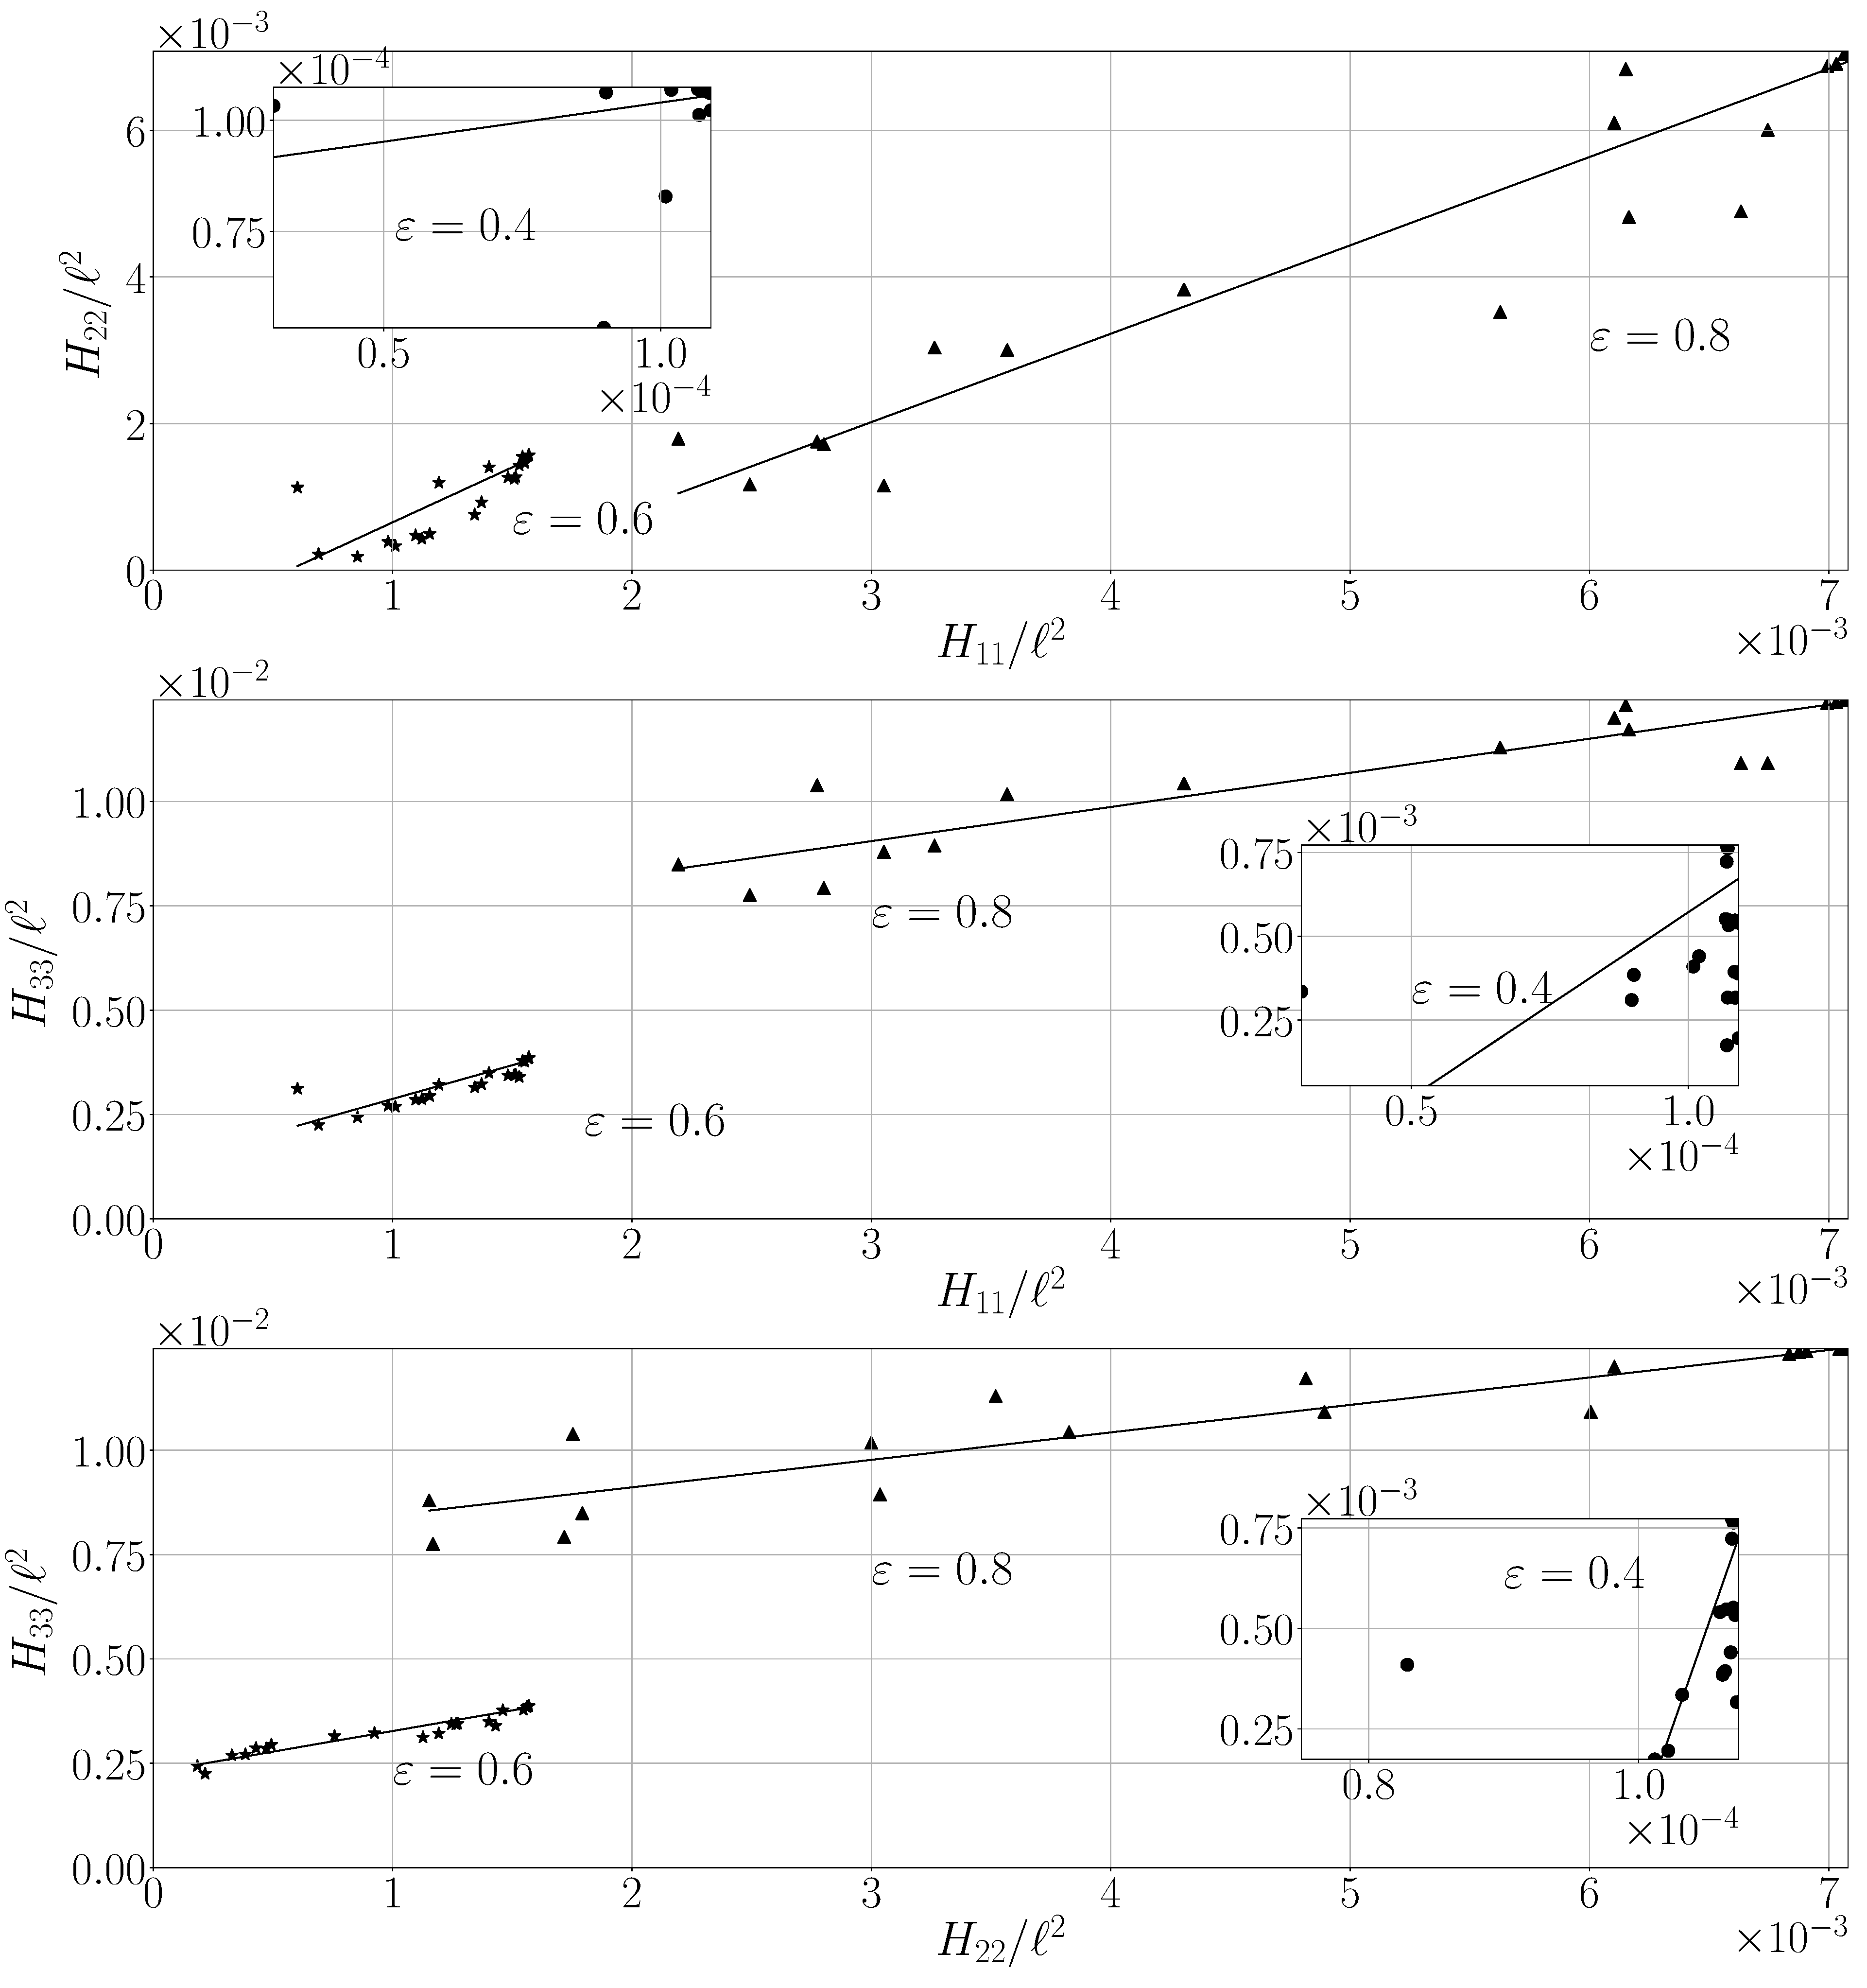
\includegraphics[width=1\linewidth]{chapter_4/figure/scatter_matrix}
	\caption{Scatter matrix plot for the collected numerical data of the apparent permeability tensor.}
	\label{fig:scatter_matrix}
\end{figure}



In the scatter plot of figure \ref{fig:scatter_matrix} the three diagonal components of the permeability tensor are shown 
as function of one another. The three porosities are separately considered in each of the above plot, and the permeability points are 
represented with their linear regression on top. This kind of plot is common in statistical analysis to determine if correlations in the data 
are present.  The permeability components show some correlation with the data points which lie reasonably well on a straight line. This
result has a physical implication.
Remembering the diagonal dominance of the permeability tensor, we have in the low
$Re_d$ limit: 

\begin{equation}
\left( \meani{u_{\beta}},\meani{v_{\beta}} , \meani{w_{\beta}}\right) \sim \left(H_{11} \dfrac{{\partial p}}{\partial x_1}, H_{22} \dfrac{{\partial p}}{\partial x_2} ,  H_{33} \dfrac{{\partial p}}{\partial x_3}\right).
\label{eq:linear_k}
\end{equation}
$$ \, $$
\noindent It is then possible to compute the angle between the forcing term, $\nabla p$, and the average velocity vector, represented 
in  figure \ref{fig:diag_rel} for the two-dimensional case, $\phi = 0$. This is achieved by taking the ratio between the
first two components of Darcy's equation, calling $\gamma$ the flow deviation with respect to the mean forcing. We thus have:

\begin{equation}
\tan \, (\theta + \gamma) = \dfrac{H_{22}}{H_{11}} \tan \, \theta.
\label{eq:angles}
\end{equation}

\noindent If the ratio between the two permeability components is equal to one, the angle $\gamma$ vanishes.
The correlation between $H_{11}$ and $H_{22}$ controls the deviation of the flow in the $(x_1, x_2)$ plane, and the argument
can easily be extended to $H_{11}/H_{33}$ and $H_{22}/H_{33}$  for deviation angles in three-dimensions.

\begin{figure}[H]
	\centering
	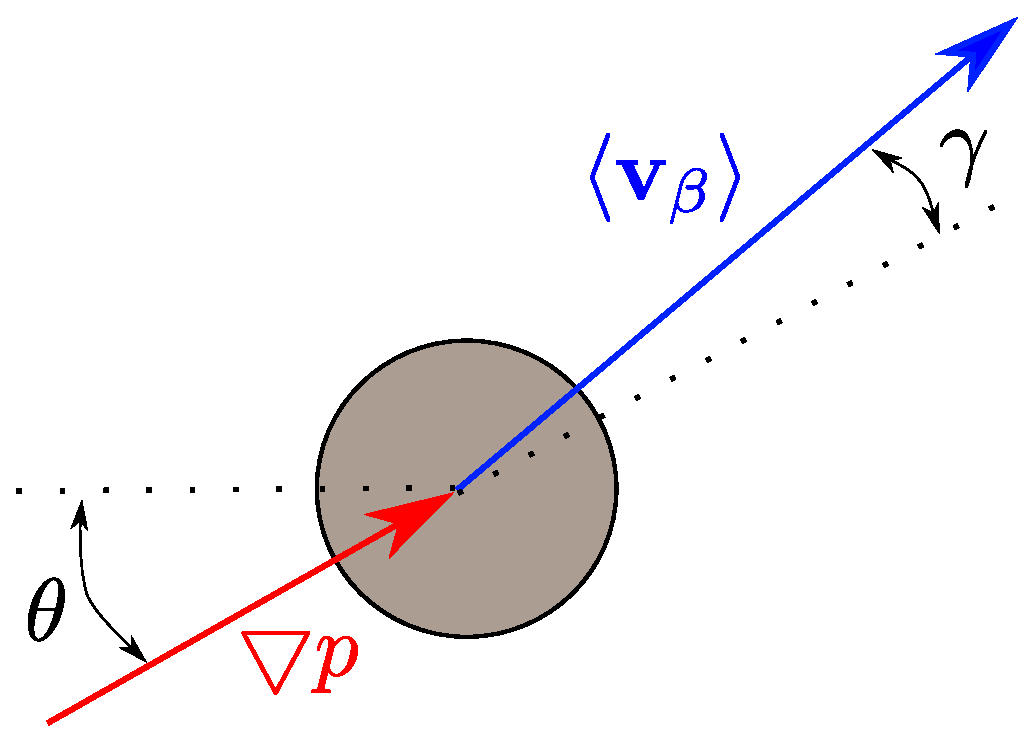
\includegraphics[width=0.45\linewidth]{chapter_4/figure/k11_k22_relation}
	\caption{Explanatory sketch for the relation between mean pressure gradient and mean velocity field.}
	\label{fig:diag_rel}
\end{figure}


\begin{table}[t]
	\centering
	\begin{tabular}{ l | l   l   l   }
		$\varepsilon$ & $H_{11}/H_{22}$ \hs{1} & $H_{11}/H_{33}$ \hs{1} & $H_{22}/H_{33}$ \hs{1} \\ \hline \hline
		0.4 & 1.57 & 11.06 & 96.03 \\ 
		0.6 & 1.50 & 1.62 & 0.99 \\
		0.8 & 1.20  & 0.82 & 0.66 \\ \hline
	\end{tabular}
	\caption{Permeability components ratio for three values of the porosity. The permeability ratios here are given by the angular coefficients of the linear correlations displayed in figure \ref{fig:scatter_matrix}.}
	\label{table:ratio}
\end{table}

Using a linear correlation such as that shown in table \ref{table:ratio} and  figure \ref{fig:scatter_matrix}, it is 
observed that in the low porosity case $(\varepsilon=0.4)$ the ratio can become very large indicating a strong deviation of the flow from the forcing direction, because of the strong constraint provided by the inclusions. As the porosity increases, the ratio does not differ much from unity, which means that the deviation remains limited. It is simple to see that
the deviation angle, for example in the $(x_1, x_2)$ plane, satisfies the approximate relation
$$
\tan \, \gamma = \dfrac{\left(1 - \dfrac{H_{11}}{H_{22}}\right) \tan \, \theta}{\dfrac{H_{11}}{H_{22}} + \tan^2 \, \theta},
$$
so that for $\dfrac{H_{11}}{H_{22}}$ equal to, say, 1.5, the largest deviation remains always below $12^{\circ}$ for any $\theta$.
It should however be kept in mind that trends based on these ratios are valid only as long as Darcy's law and linear correlations
are acceptable. Cases exists for which such trends are violated; for example, a flow with $\theta = 45^{\circ}$ and $\phi = 0^{\circ}$ has
deviation angle $\gamma$ equal to zero, for whatever porosity. In this case $H_{11}/H_{22}$ is equal to one and such a point is an 
outlier in the regression plots of figure \ref{fig:scatter_matrix}.


%%%%%%%%%%%%%%%%%%%%%%%%%%%%%%%%%%%%%%%%%%%%
\subsection{Kriging interpolation method}
%%%%%%%%%%%%%%%%%%%%%%%%%%%%%%%%%%%%%%%%%%%%

The kriging approach is a linear interpolation/extrapolation method that aims to build a predictor field
based on a set of observations  $(\mathbf{x_i}, y(\mathbf{x_i}))$,  for $i=1,...,n$. 

The predictor $\hat{f}(\mathbf{x})$ is a sum of a trend function $t(\mathbf{x})$ and a Gaussian process error model $e(\mathbf{x})$:
\begin{equation}
\hat{f}(\mathbf{x}) = t(\mathbf{x}) + e(\mathbf{x}).
\label{eq:Kriging}
\end{equation}
The aim of the error model is to make adjustments on the trend function so that,
for any point of the sampling
%, equation \eqref{eq:Kriging} is strictly verified,
the predictor is  exactly equal to the sample, 
i.e. $\hat{f}(\mathbf{x_i}) = y(\mathbf{x_i})$. This property represents one of the main qualities of this approach. In addition, 
when  the model parameters are  conveniently  set,  the trend function and the covariance model can take into account both smooth and steep variations in the data set.


The trend function defined  here is  based on a second order least-square regression, with the coefficients found from 
the solution of the associated linear system.
The Gaussian process error model has zero-mean and its covariance between two generic data-points, $x_i$ and $x_j$, is written as 
$$
\textrm{Cov}(y(\mathbf{x_i}), y(\mathbf{x_j})) = c(\mathbf{x_i}, \mathbf{x_j})
$$
The function $c(x^i, x^j)$ is a correlation model, based on the Mat\'ern covariance model that reads:
\begin{equation}
c(\mathbf{x_i}, \mathbf{x_j}) = \sigma^2 \dfrac{2^{1- \nu}}{\Gamma(\nu)} \  \left( \dfrac{\sqrt{2} \nu |\mathbf{x_i} - \mathbf{x_j}|}{|\bs{\lambda}|} \right)^{\nu} \ K_{\nu}\left( \dfrac{\sqrt{2} \nu |\mathbf{x_i} - \mathbf{x_j}|}{|\bs{\lambda}|} \right),
\label{eq:matern}
\end{equation}
where $K_{\nu}(.)$ is a modified Bessel function, $\Gamma(.)$ is the gamma function and the coefficient $\sigma$ is an amplitude parameter.
The parameters that can be used to tune the metamodel are the amplitude parameter $\sigma$, the exponent $\nu$ and the scale vector $\bs{\lambda}$.
The kriging metamodel outputs can show different behaviours for different selections of the above three parameters and their setting is thus crucial. 
The amplitude parameter $\sigma$ is chosen to be equal to $1$; larger value lead to steeper gradients and undesirable local extrema around the data points.
The vector $\bs{\lambda}=(\lambda_{\theta}, \lambda_{\phi}, \lambda_{Re_d}, \lambda_{\varepsilon} )$ is a scaling parameter for the distance $ |\mathbf{x_i} - \mathbf{x_j}|$.
In this study, through systematic variations of the parameters it is found that  the choice $\bs{\lambda}=(1.2, 1, 1, 1)$ yields acceptable results; in particular, the weight along $\theta$ 
is mildly larger than in the other directions in order to obtain smoother metamodel surfaces in this direction.
The exponent $\nu$ controls the  covariance function and more especially its gradients. 
When  $\nu = 1/2$ the covariance can be approximated by a negative exponential, $\exp(-\alpha x)$  and  when $\nu$ goes to infinity it behaves as $\exp(-\alpha x^2)$.
In the present study, the best (i.e. smoother) results are obtained for $\nu$ equal to $1.9$.
The above parameters have been chosen in order to avoid unphysical or unrealistic  behaviour of the apparent permeability such as, for instance,  negative values or 
steep, spurious local maxima/minima.
The method above is implemented in OpenTURNS and full details are provided by \citet{openturns}. 


A procedure called \textit{k}-fold, belonging to the class of cross-validation methods, has been used in order to prove the robustness of the metamodel.
The \textit{k}-fold method starts with the full database $S_n = (\mathbf{x_i}, \mathbf{y}(\mathbf{x_i}))$,  for $i=1,...,n$, split into two complementary set of size $n_1$ and $n_2$, such that $S_n = S_{n_1} \cup S_{n_2}$.
Then, a new metamodel is built using only the points present in the set $S_{n_1}$. 
For the sake of clarity, the metamodel built with only the subset $S_{n_1}$ will be called from now on $\hat{f}^{n_1}$, and the metamodel build with all the database will be indicated as $\hat{f}^{n}$.
The idea now is to use the points in the set $S_{n_2}$ as test, since they are essentially "new" for the metamodel $\hat{f}^{n_1}$.
The division of the subset is performed picking points in a random way, and is repeated $k$ times in order to rule out any possible "lucky" combination.

Thus, the metric used for the error computation is the following:
$$
\xi_{cv} = \dfrac{1}{k \; n_2}\sum_{i = 1}^{k} \sum_{j = 1}^{n_2} (\hat{f_{i}}(x_j)^{n} -\hat{f_{i}}(x_j)^{n_2} )^2 ,
$$
quantifying the quadratic error between the original metamodel and the one built each time with a different set that belongs to different folds.
The metric is also averaged over all the test points $n_2$ present in all the \textit{k} folds. 
The relative mean error can be computed as:
$$
E_{cv\%} = 100 \dfrac{\sqrt{\xi_{cv}}}{mean(|\hat{f_{i}}^{n}|)} .
$$
In our case the number of points used to test the model $n_2$ is equal to $\sqrt{N} \approx 12$ as recommended for kriging metamodels \citet{wang2007review}.
The number of folds has been varied from $5$ to $25$ and in all the cases tested the $E_{cv\%}$ has been found to decrease below $6\%$ when we use at least 16 folds (which means leaving out 7 to 8 points from the metamodel construction), which is more than acceptable to prove that our kriging method is a robust approximation.

\begin{figure}[h]
	\centering
	\includegraphics[width=0.7\linewidth]{chapter_4/figure/kfold_err}
	\caption{Relative mean error computed using the \textit{k}-fold approach presented against the number of folds $k$ used to divide the
		dataset}
	\label{fig:kfold_err}
\end{figure}


The metamodel provides a scalar function (for each term of the $\mathbf{H}$ tensor) defined in a four-dimensional space.
In each of the following figures  two parameters are fixed and the response surface is displayed as function of the remaining two, focussing on the  $H_{11}$ component. 
The other diagonal components of the apparent permeability tensor behave in a similar fashion and will not be shown for brevity. All the results of the metamodel are,
however, available from the authors upon request.


\begin{figure}[t]
	\centering
	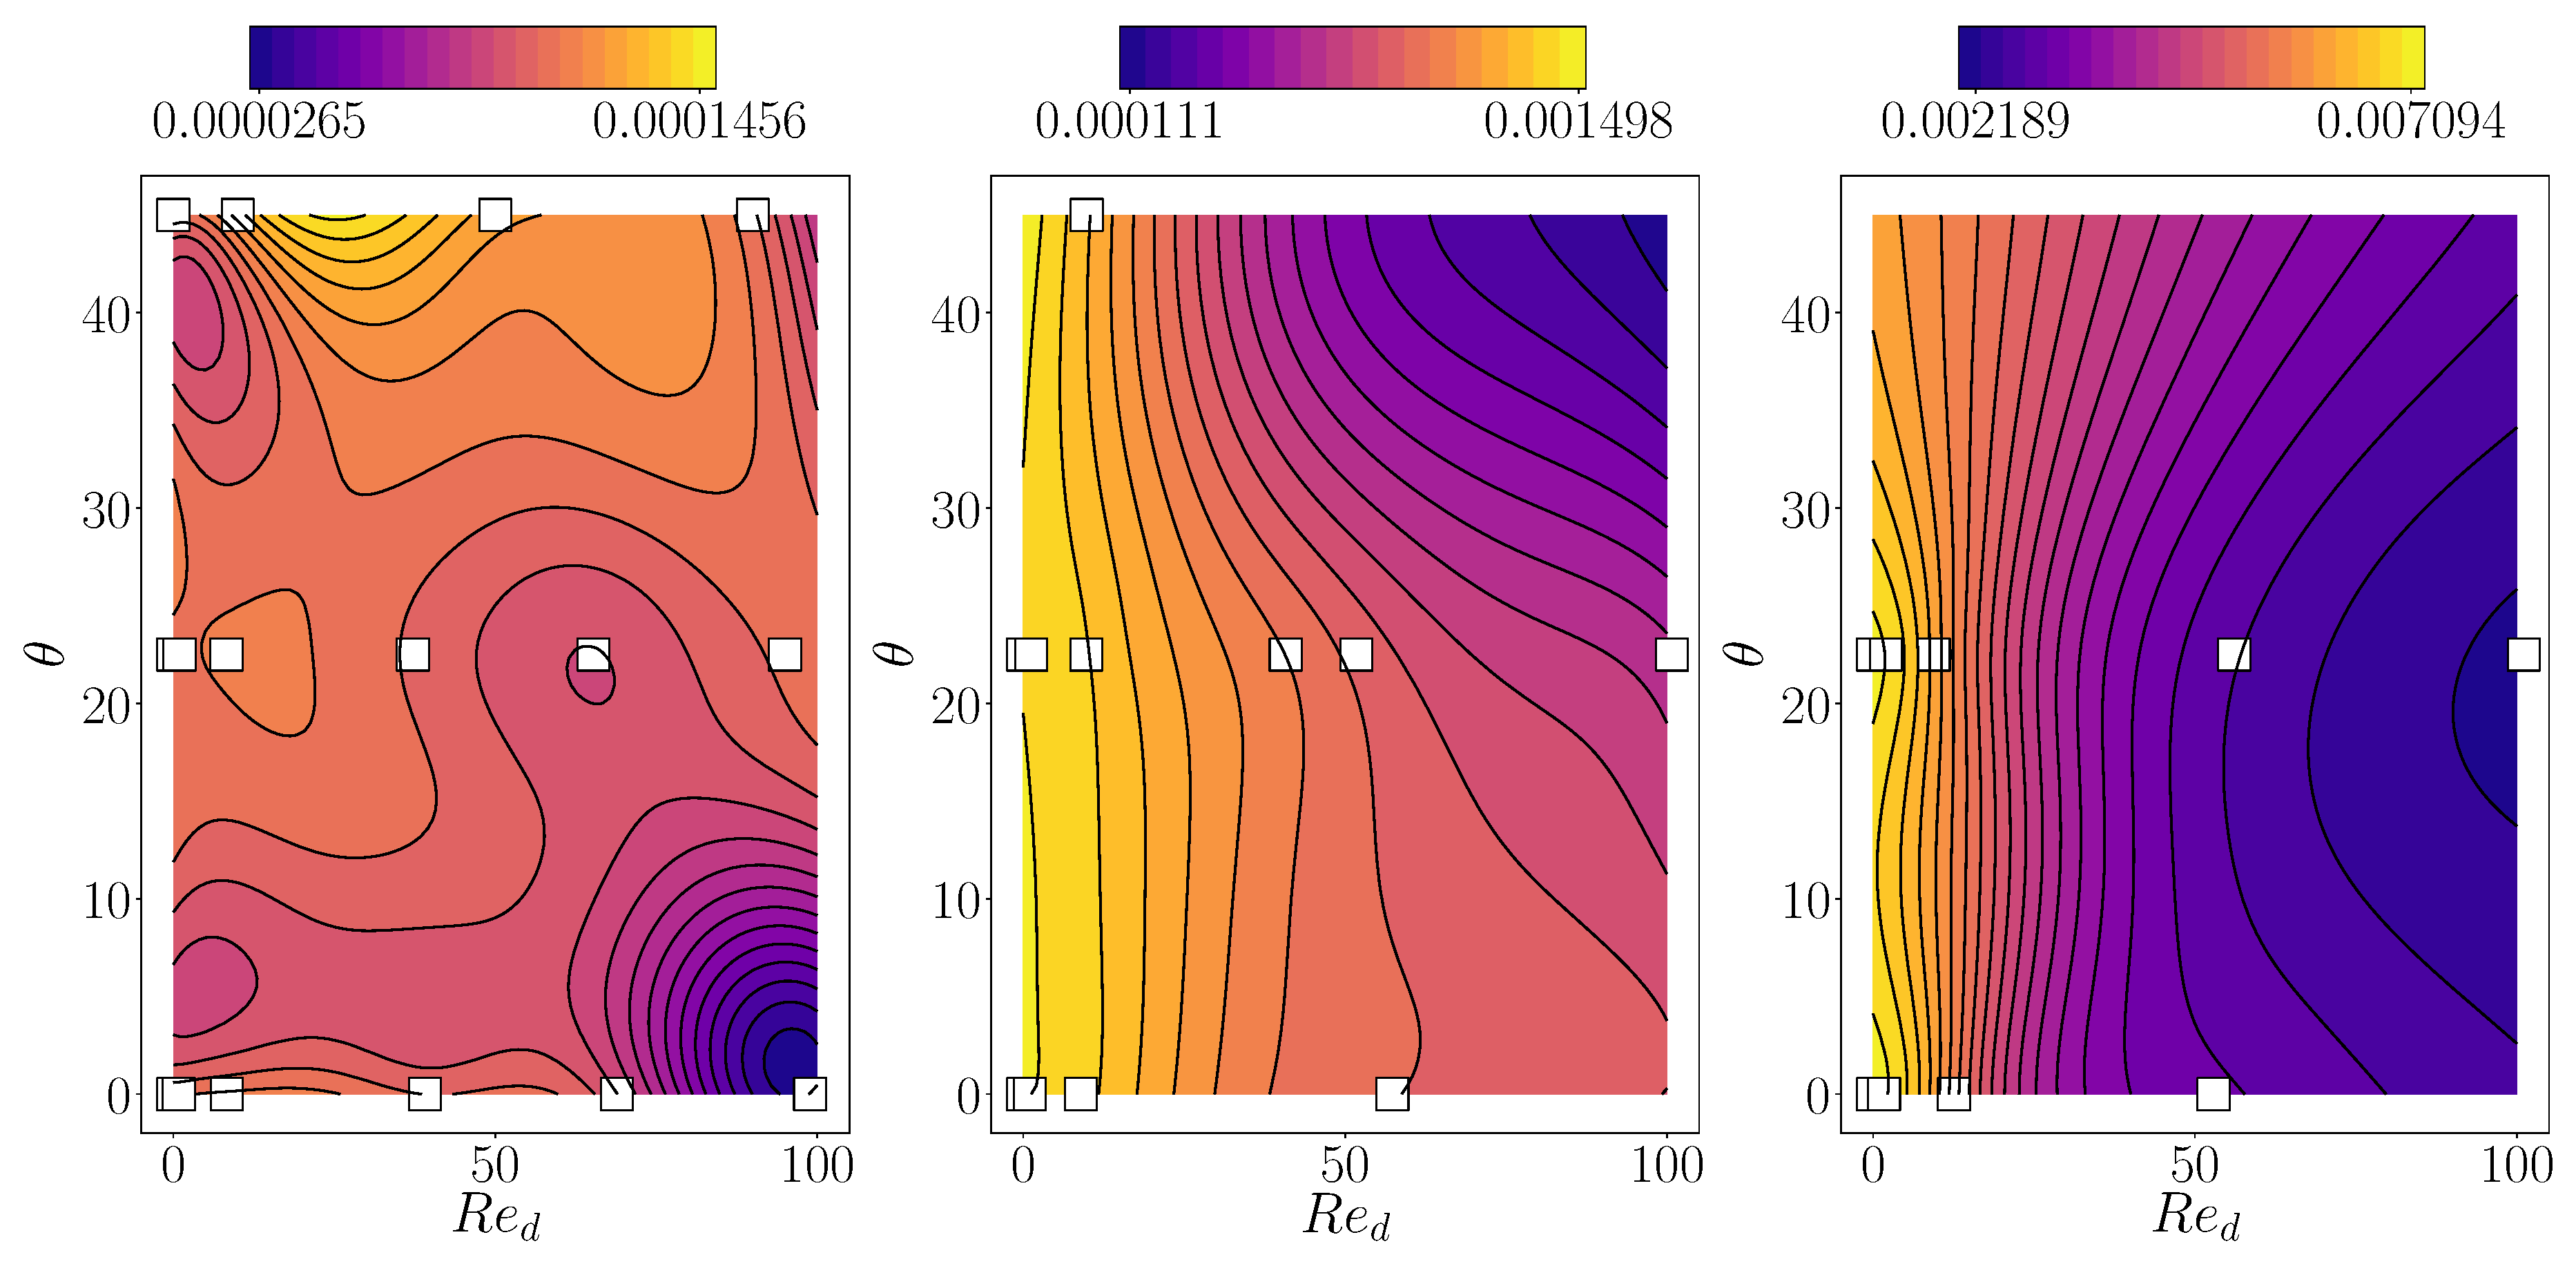
\includegraphics[width=1\linewidth]{chapter_4/figure/krig_mater_th_re}
	\caption{Response surfaces of $H_{11}$ with $\phi=0^{\circ}$ for porosity $\varepsilon=0.4, 0.6, 0.8$, from left to right.}
	\label{fig:th_re}
\end{figure}


In figure \ref{fig:th_re} the angle $\phi$ is fixed to zero, and the isolines display $H_{11}$ as function of the angle $\theta$ and of the 
Reynolds number, $Re_d$, for three  values of porosity.  The white square symbols indicate the  samples used to build the metamodel. The maximum value of 
each surface is always found for $Re_d$ equal to zero and  $H_{11}$  typically decreases with $Re_d$, when the porosity is sufficiently large.
As seen previously, for a porosity approximately greater or equal to 0.6 the variation of the  apparent permeability with the angle $\theta$ 
is weak in this two-dimensional configuration.
For the  lowest porosity studied (left frame)  the permeability has very small values and the isolines display an irregular behaviour; this is a feature
common to all plots relative to the smaller value of $\varepsilon$, signaling that it is probably necessary, in this specific case, to insert additional sample 
points in building the response surfaces. 
%Steep gradients with $Re_d$ are displayed  in the case of horizontal flow ($\theta = 0^{\circ}$).
%The observations made upon inspection of the figure are essentially the same presented in section \ref{sec:5}, and this is comforting, since it leads to
%believe in the  capacity of the metamodel to describe the trend of $H_{11} = f(\theta, Re_d)$.



\begin{figure}[t]
	\centering
	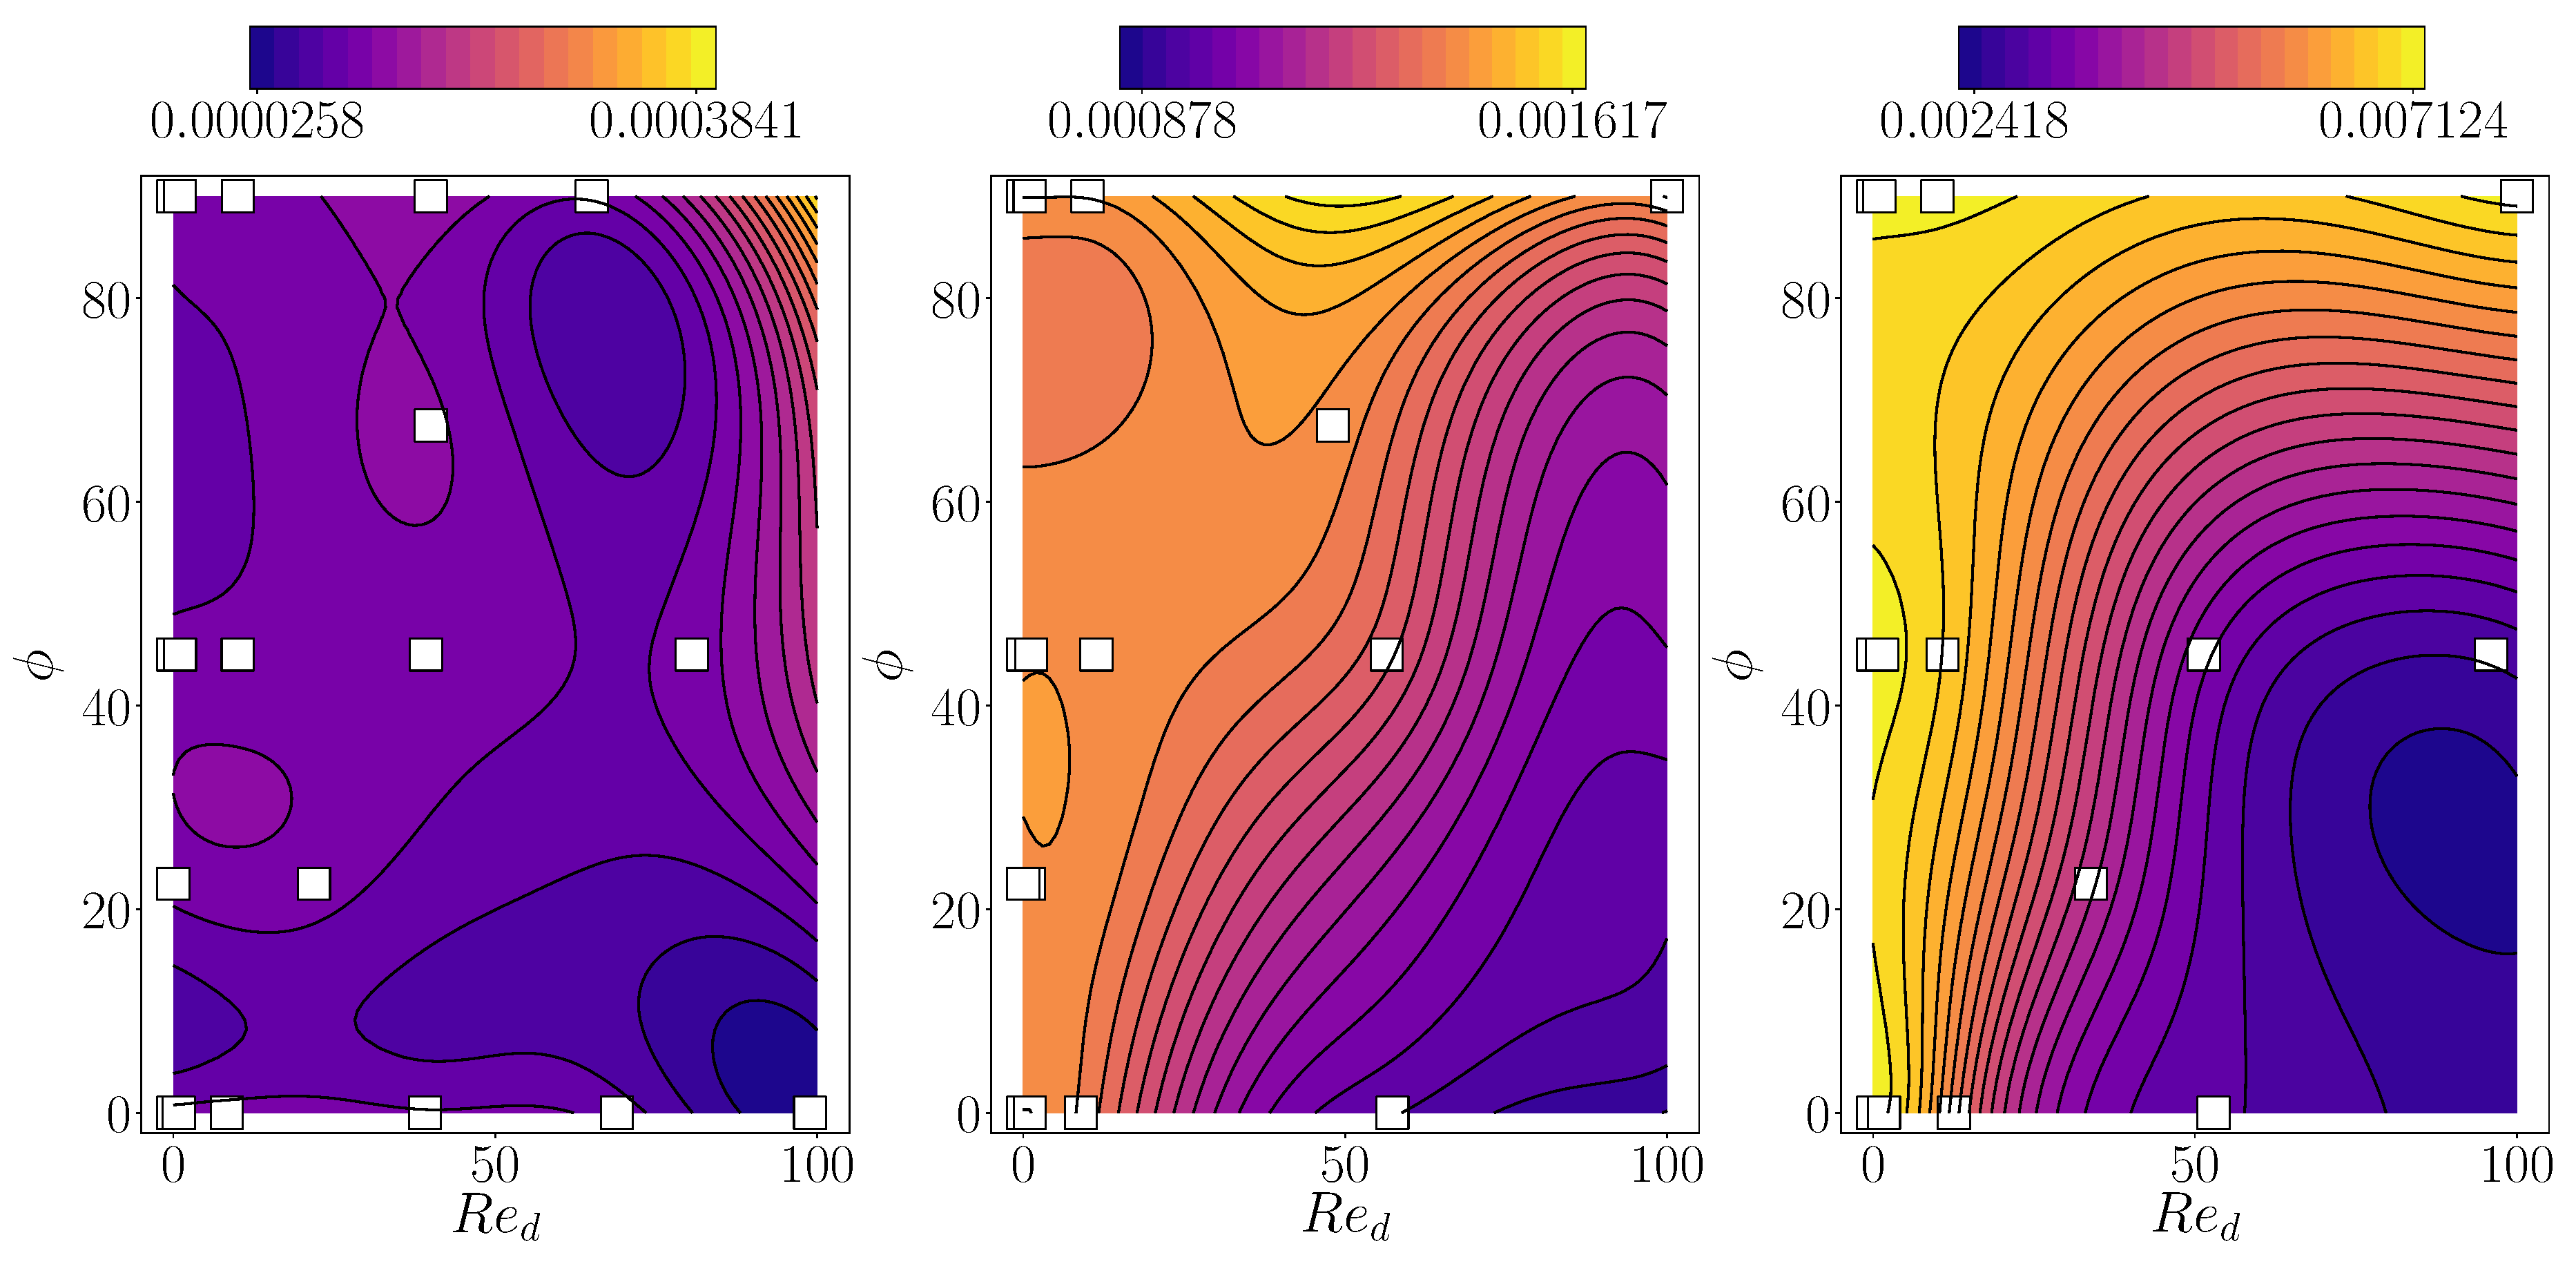
\includegraphics[width=1\linewidth]{chapter_4/figure/krig_mater_ph_re}
	\caption{Response surfaces of $H_{11}$ with $\theta=0^{\circ}$ for porosity $\varepsilon=0.4, 0.6, 0.8$, from left to right.}
	\label{fig:ph_re}
\end{figure}


In  figure \ref{fig:ph_re} the parameter  $\theta$ is set to  $0^{\circ}$ and  the response surface is displayed in the $Re_d - \phi$ plane.
As already indicated, the results confirm that an  increase of  the Reynolds number is generally associated to  a decrease of  the first diagonal component  of the apparent permeability tensor. However, the $H_{11}$ variations with respect to $\phi$ are more pronounced than those found with respect to $\theta$ and are due to a real three-dimensionalization of the flow.
This conclusion remains to be verified in the lower porosity case (left frame) where the variations are very tiny and more irregular.

%For the porosity equals to $0.8$, the surface becomes wavy  around $Re_d = 50$ region. It could be due to the lack of sampled point at this %higher range of Reynolds number. 
%In this region  the surface with porosity equals to $0.6$  shows a more regular variation. Some additional sample could help to explain the %different behaviours.




\begin{figure}[t]
	\centering
	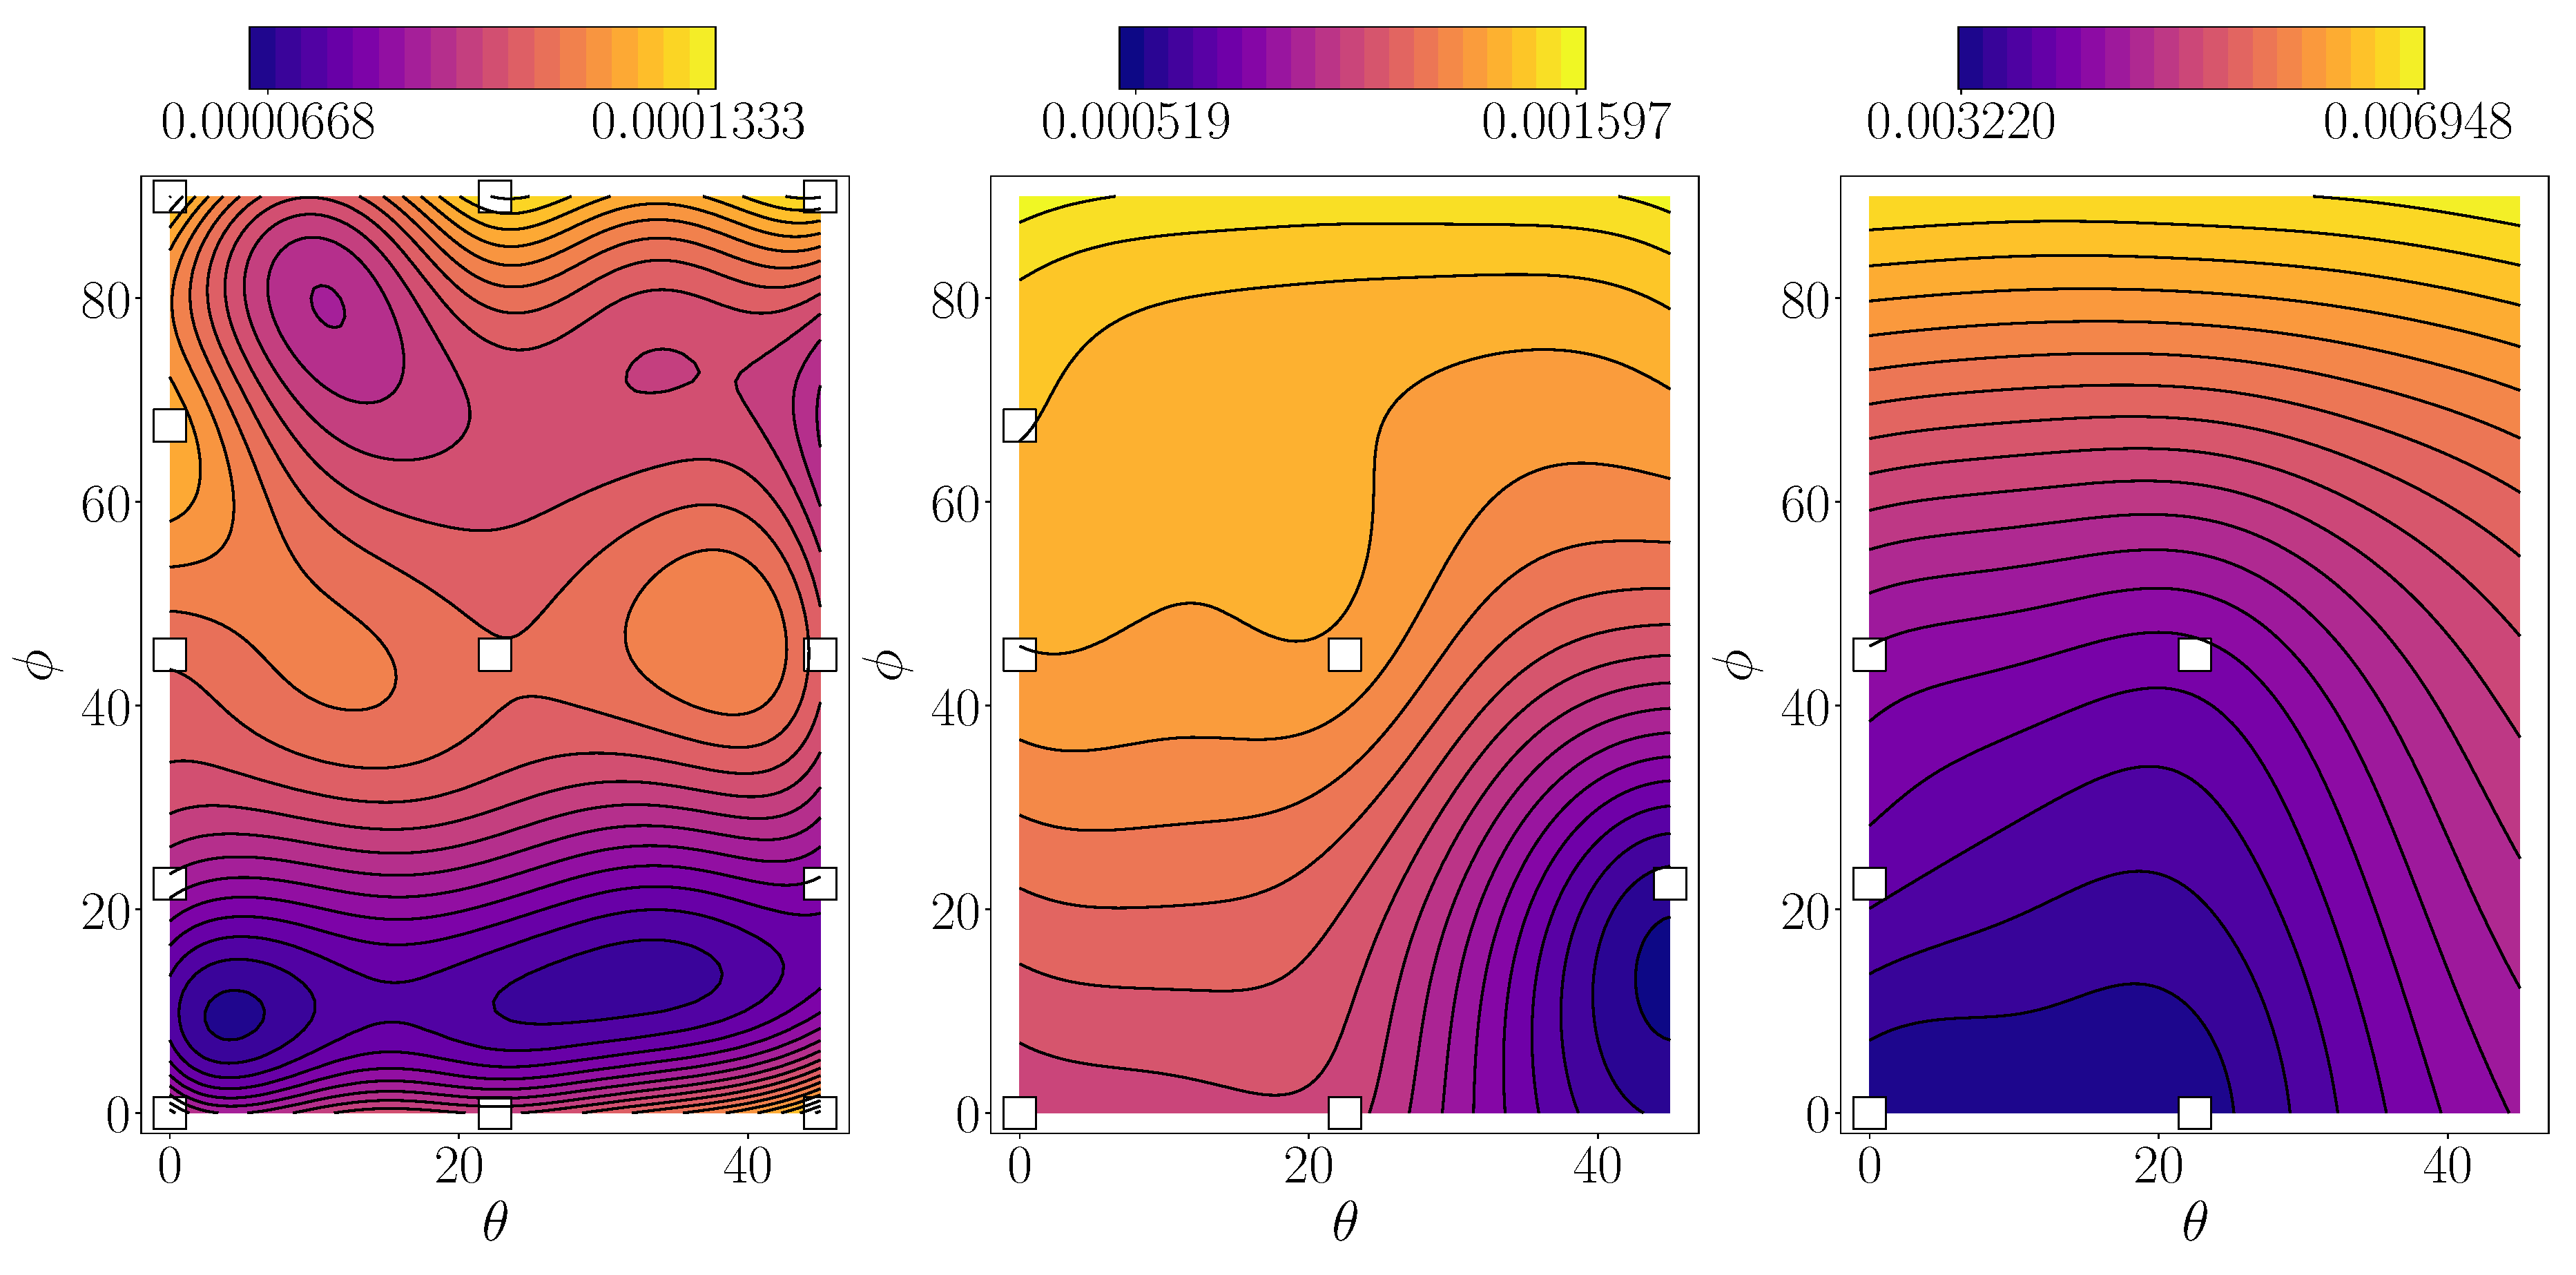
\includegraphics[width=1\linewidth]{chapter_4/figure/krig_mater_th_phi_re40}
	\caption{Response surfaces of $H_{11}$ with $Re=40$ for porosity $\varepsilon=0.4, 0.6, 0.8$, from left to right.}
	\label{fig:th_ph}
\end{figure}


In figure \ref{fig:th_ph} the Reynolds number is set to the inertial range value of $40$ and  the response surface 
is displayed in the $\theta - \phi$ plane. 
For the two highest porosity values, $0.6$ and $0.8$, the results confirm that $H_{11}$ has a much stronger dependence on
$\phi$ than on $\theta$, suggesting that the real test of permeability models must include three-dimensional effects.
As seen earlier, the behaviour of the permeability when the porosity is low (left frame in the figure) is not intuitive, with 
a significant effect of the angle $\phi$ and a minor influence of $\theta$. Again this occurs
from the constraint provided to the flow by the inclusions, and from the occurrence of a large deviation $\gamma$ in these cases.

%shows a strong variability with respect to the angle $\phi$  and a weak one with respect to the angle $\theta$.
%At given Reynolds number the permeability does not depend (too much) of the flow direction in the horizontal plane.
%These conclusions are in agreement with the one observations written in section \ref{sec:4}.

%For the lowest porosity $0.4$ the complex behaviours are retrieved. With respect to the other porosity the variations are inverted : 
%a strong variability with respect to the angle $\theta$ and a weak one with respect to $\phi$ are found.
%As earlier  stated in the previous sections,  with a low porosity the flow direction is deflected towards the fiber axis direction with the %tri-dimensional flow.

%In the range of $\phi < 25^{\circ}$ where the tri-dimensionality remains small  the surface response exhibit a plateau in range $\theta \in %[10^\circ \  30^\circ ]$. The existence
%of this plateau remains unexplained.





The response surface is shown in the $Re_d - \varepsilon$ plane of figure \ref{fig:por} for three sets of $\theta-\phi$ angles. 
Here a significant effect of the porosity with respect to  the Reynolds number is obervable. 
In fact  the surface  gradient is almost aligned with the porosity direction, i.e. a quasi- Reynolds independence is demonstrated  in this plane,
and  the apparent permeability can change by one order of magnitude in the range
of the analysed porosity.

Some relatively small Reynolds number effects are visible at porosity equal to $0.8$, when the wake of the flow has more space to develop in the inertial regime.
In the central figure the flow is aligned with the direction of the fibers and, as expected, it shows practically no dependence with respect to the Reynolds number.


The response surface analysis has confirmed the qualitative trends which had been reached earlier on the basis of a few selected 
flow cases, yielding at the same time much more detailed information on the behaviour of the apparent permeability with the
parameters of the problem. The data base which has been built will be used in future work which will focus, via the VANS approach,
on configurations for which neither the porosity nor the local Reynolds number are constant in space or time.

\begin{figure}[t]
	\centering
	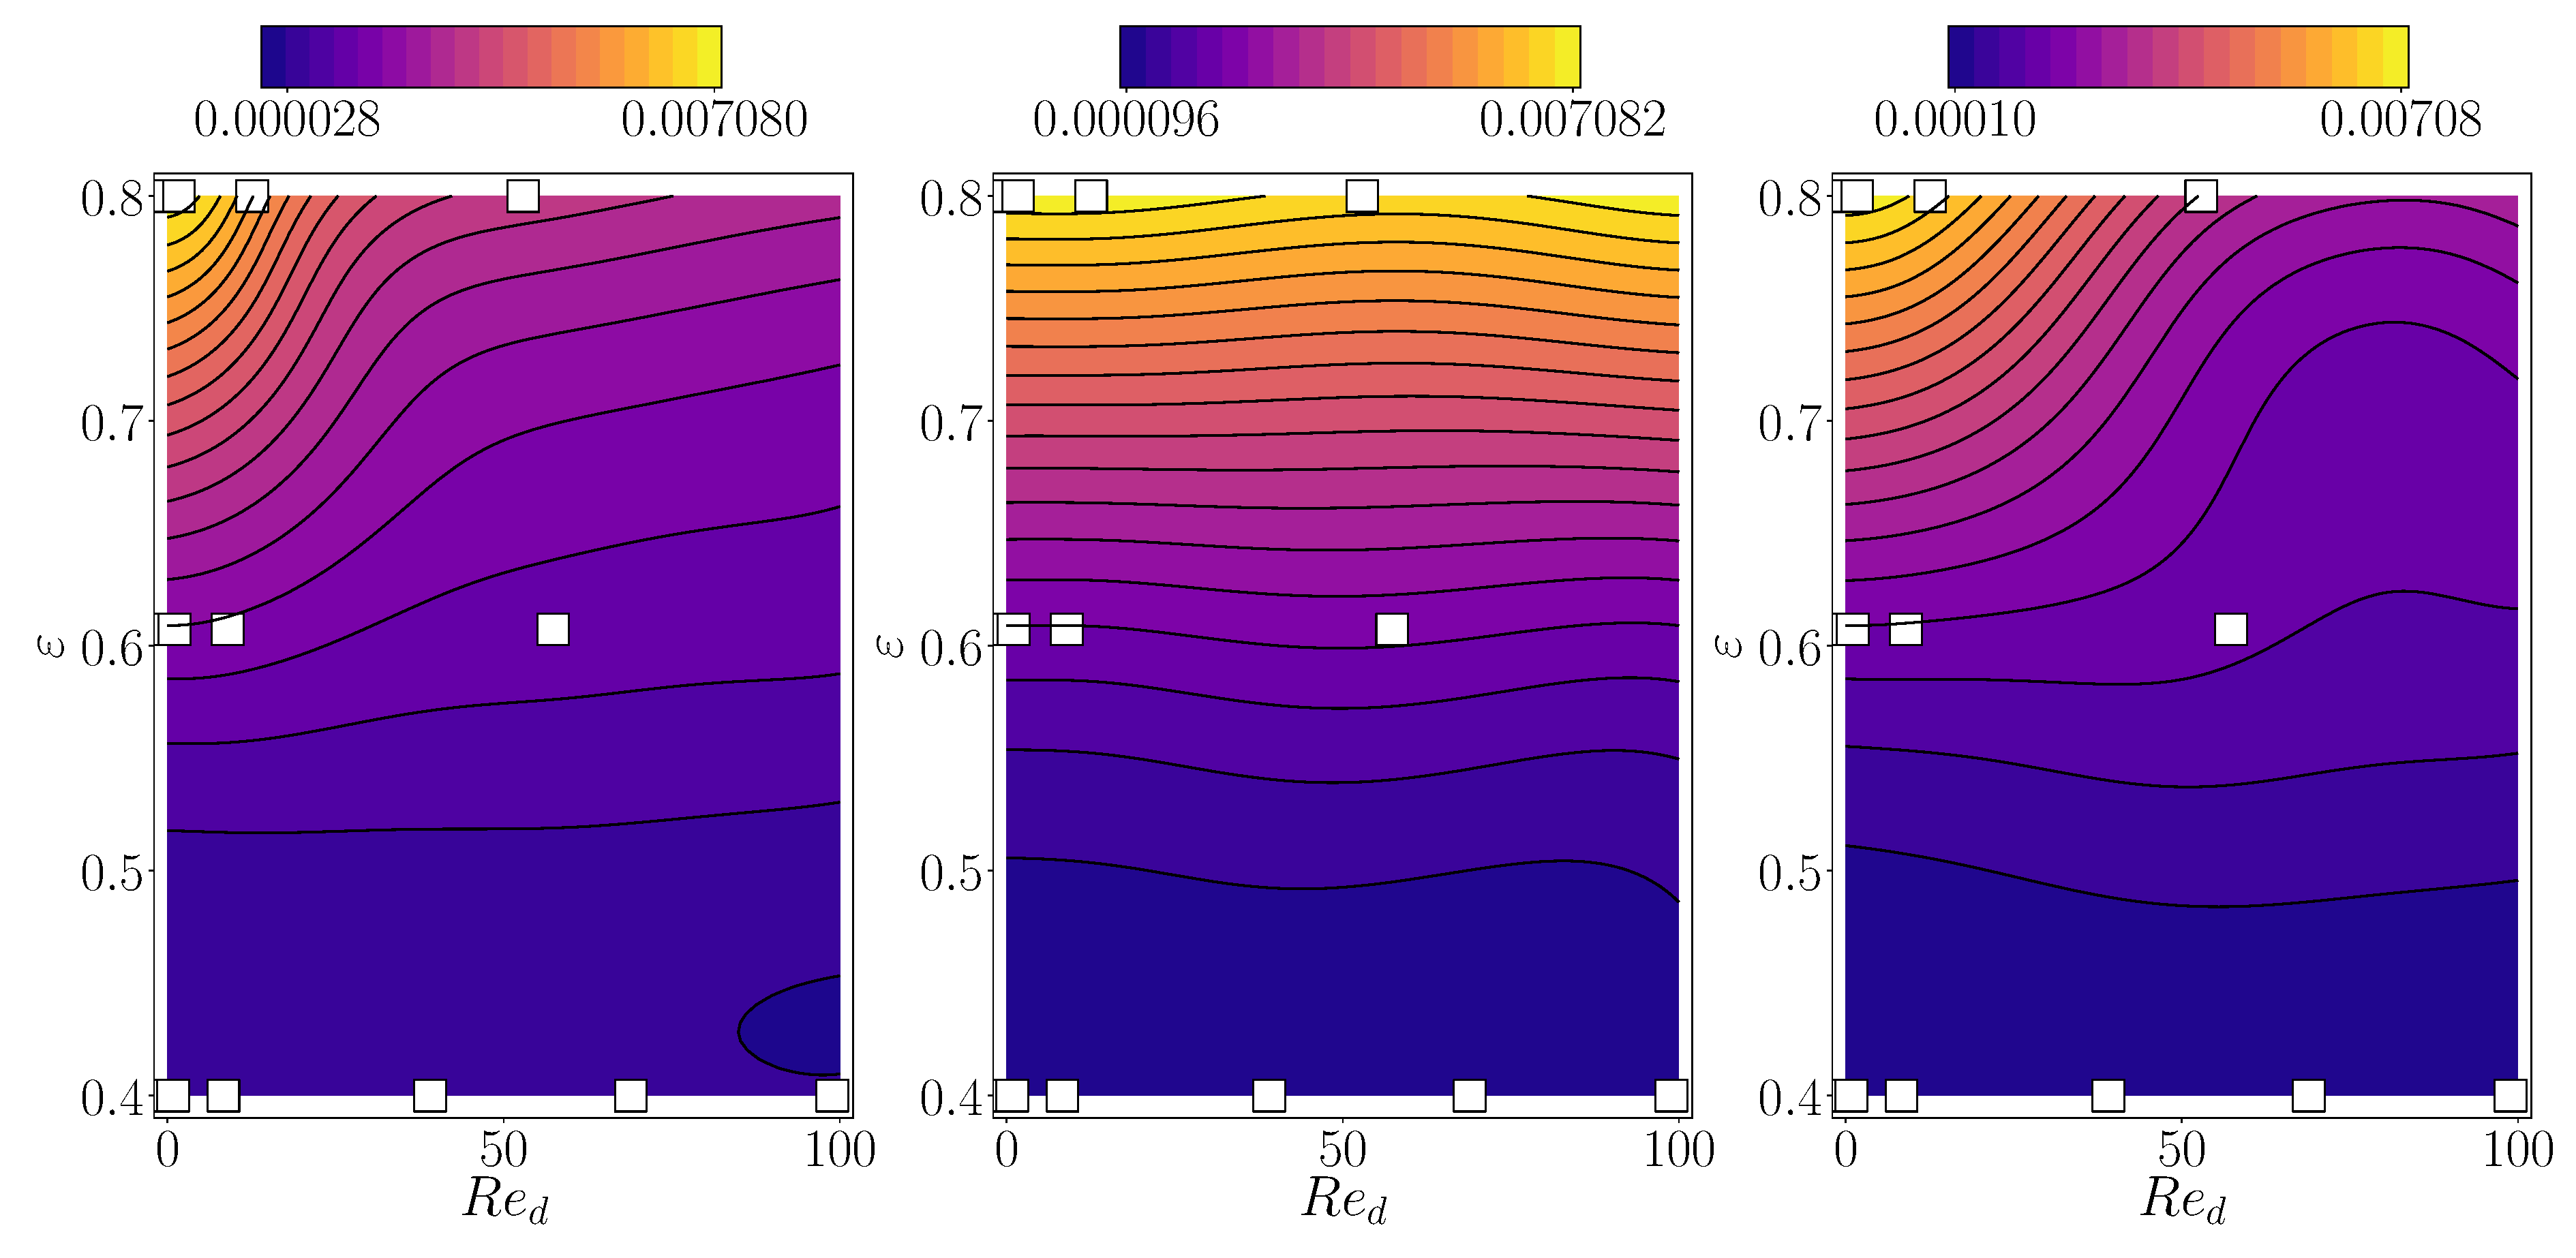
\includegraphics[width=1\linewidth]{chapter_4/figure/krig_mater_eps_re}
	\caption{Response surface of $H_{11}$; in the left frame $\phi= \theta = 0$, in the centre frame $\phi=90^{\circ}$, $ \theta = 0$ and on the right $\phi= 45^{\circ}$, $ \theta = 22.5^{\circ}$.}
	\label{fig:por}
\end{figure}

For the sake of space, only the first diagonal component of the apparent permeability tensor has been discussed 
in detail; however, all components have been computed and the same conclusions can be drawn from the $H_{22}$ or $H_{33}$ component.


%%%%%%%%%%%%%%%%%%%%%%%%%%%%%
\section{Concluding remarks}
%%%%%%%%%%%%%%%%%%%%%%%%%%%%%

The components of the permeability tensor are essential ingredients for any solution of flow
through anisotropic porous media.  When the flow through the pores resents of significant
acceleration effects, the permeability must be modified (it is then called \emph{apparent}) by the presence
of a second tensor, the Forchheimer tensor $\mathbf{F}$, defined by   
$$
\mathbf{F} =  \mathbf{K} \mathbf{H}^{-1} - \mathbf{I}.
$$
The permeability, $\mathbf{K}$, and the apparent permeability, $\mathbf{H}$, can be formally deduced by two closure problems which have
been briefly recalled in section \ref{sec:2ch4}.  The real obstacle to the solution of the problem for $\mathbf{H}$ is the need
to know the microscopic velocity fields through the pores. We have solved for such fields 
in a unit cell (the REV), varying the forcing amplitude and direction, treating over one
hundred different cases of flows through arrangements of parallel fibers. From this, we have
thus been able to solve the linear system \eqref{eq:linear_k} for all the unknown elements of the 
intermediate tensor  
$\mathbf{M}$, from which, through averaging, we have computed the apparent permeability.  Such a tensor
is  indispensable to evaluate accurately the drag force caused by the presence of the fibers, for a macroscopic solution of the flow on the
basis of equations \citet{whitaker2013method} when inertial effects are present.

It has been found that the apparent permeability tensor is strongly diagonally dominant for whatever
forcing direction and porosity,  provided the local Reynolds number remains below a value 
approximately equal to 100; this results (which is a direct
consequence of the transverse isotropy of the material which has been considered here) 
can be used to compute $\mathbf{H}$ rapidly, approximating it as a diagonal tensor.

Finally, a metamodel has been used to produce results so as to cover the whole space of parameters,
and this has allowed the construction of a complete data base. This database can be used in simulations of porous media based on the VANS approach as we will show in the next chapter. 

\chapter{VANS macroscopic applications}

\chapquote{The first principle is that you must not fool yourself — and you are the easiest person to fool.}{1974 Caltech commencement address}{Richard Feynman}

\section{Introduction}

In this last chapter the macroscopic VANS equation are validated against a full microscopic DNS. Special attention is focused on the interface treatment using the penalization method. We also assess the effects of the permeability tensor metamodel introduction in the algorithm. The computation is performed using the classical  closed cavity configuration. The aim for the cavity problem is to validate the VANS approach and show the importance of the interface treatment and the permeability metamodel. In the last part the Ercoftac periodic hill case is also tested. This open configuration aim to test the performance of porous coating as a device that helps to reduce separated flow.


\section{Closed cavity problem}
The configuration chosen is the squared closed cavity, depicted in figure \ref{fig:geom}.
The cavity is square shaped with size $L$, the lateral and bottom walls are fixed and a constant velocity $U_{top}$ is specified at the top side.
On the front and back side we apply periodic boundary condition since the simulation domain has a depth equal to $\ell$.
A rigid porous media made by regularly arranged fibers is set at the bottom of the cavity, its vertical extension is equal to $h$.
The \textit{reference elementary volume} (REV) of the porous medium is a cubic cell of size $\ell$ with a cylinder, with diameter $d$, at his center.
The permeability of the medium $\varepsilon$ is equal to 0.8 and with 50 fibers in the cavity.

\begin{figure}[h]
\centering
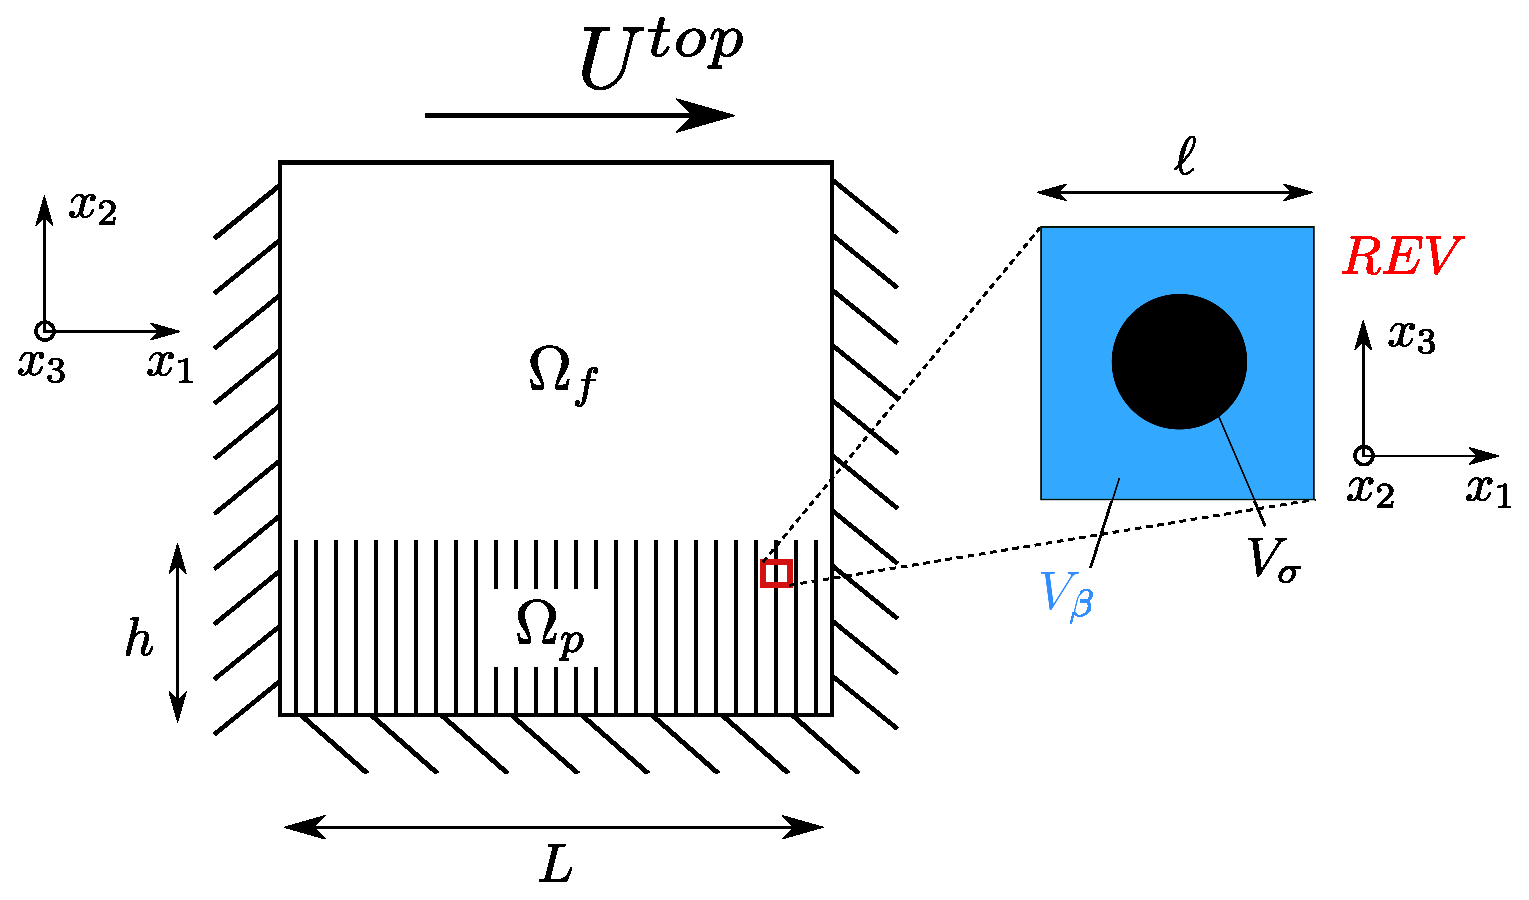
\includegraphics[width=0.7\linewidth]{chapter_5/figure/cavity_draw.eps}
\caption{Schematics of the closed cavity 2D problem. The porous medium internal structure is depicted in the zoom on the right side in which the REV geometry is showed.}
\label{fig:geom}
\end{figure}

To summarize the configuration:
\begin{itemize}
	\item $L$: side of the cavity, also the macroscopic length scale
	\item $h$: vertical extension of the fibers from the bottom of the cavity 
	\item $\ell$: side of the cubic REV, also the microscopic length scale
	\item $d$: diameter of the cylindrical fiber
	\item $V_{\beta}$: volume of the fluid inside the REV
	\item $V_{\sigma}$: volume of the solid inside the REV
	\item $\varepsilon = \dfrac{V_{\beta}}{V_{\sigma} +V_{\beta}}$: porosity of the medium
	\item $\epsilon = \dfrac{\ell}{L}$: length scale ratio
	\item $Re= \dfrac{U_{top} L}{\nub}$: Reynolds number of the cavity
\end{itemize}

The overall domain has the size $L \, \times \, L \times \, \ell$ respectively in the $x_1$, $x_2$ and $x_3$ directions. The origin of our coordinate system at the bottom left corner of the cavity. 
This configuration and porous arrangement has been chosen to reuse DNS data already available for this configuration (private communication with the authors of \citet{zampogna2016fluid}).

The length parameters for the specific case are:
\begin{itemize}
	\item $h/L=0.33$
	\item $\ell/L=0.02$
	\item $\varepsilon = 0.8$
\end{itemize}

\subsection{Microscopic approach with direct numerical simulations}

In this approach the incompressible Navier-Stokes equations are solved in the three dimensional case \eqref{eq:NScavity}. 
The problem is weakly three dimensional problem since we include only one REV in the $x_3$ axes and we impose periodic boundary condition in this direction.
This assumption seems fair since the Reynolds numbers tested are small and no 3D structure are expected in the flow.
To complete the set of boundary condition the no-slip condition is applied at the rigid walls and a prescribed horizontal velocity is imposed at the top wall \eqref{eq:NScavity}. The subscript $\beta$ means that the variables belongs to the fluid phase, as usual. The mesh was fine enough to resolve the flow inside the fibers and the spatial converged is also assured.

\begin{eqnarray}
\begin{cases}
\derp{\vb}{t} + \vb \cdot \nabla \vb = -\frac{1}{\rho_{\beta}} \nabla \pb + \nub \nabla^2  \vb \\
\nabla \cdot \vb = 0\\
\vb = 0 \qquad \text{on} \quad x_1 = 0/L \quad x_3 = 0 \\
\vb = U^{top} \qquad \text{on} \quad x_3 = L\\
\vb|_{x_3 = 0} = \vb|_{x_3 = \ell}  \\
\pb|_{x_3 = 0} = \pb|_{x_3 = \ell}
\end{cases}
\label{eq:NScavity}
\end{eqnarray}

Once the system \eqref{eq:NScavity} is solved, the microscopic fields (velocity and pressure) inside the porous medium are averaged with the operator \ref{eq:supavg} in order to get the homogenized macroscopic field $\meani{\vb}$ and $\meani{\pb}$.

\begin{equation}
	\meani{\psi_{\beta}} = \dfrac{1}{\volb} \int_{\volb} \psi_\beta (\mathbf{x}) d \volb.
	\label{eq:supavg}
\end{equation}

The operator \eqref{eq:supavg} has been applied through the all porous domain using a REV with dimension $\ell \times \ell \times \ell$.
It means that the centroid of the REV, in which the average operation is performed, span all the porous domain extension.
It should be noted that the averaging procedure gives a two dimensional averaged fields as results, the only not null values are in the $x_1$ and $x_2$ directions. This is due to the symmetry of velocity and pressure in the $x_3$ direction that return null averaged field as a result of the averaging operation \eqref{eq:supavg}.

\subsection{Macroscopic approach though VANS}

The same problem is solved using the VANS approach.
The set of equation used are the incompressible Volume Averaged Navier-Stokes equations in the two dimensional case with a Darcy-Forchheimer closure \eqref{eq:vans_cav}.
The derivation of this set of equation has been already discussed in chapter 2.

\begin{eqnarray}
\begin{cases}
\derp{\vbms}{t} + \dfrac{1}{\varepsilon} \nabla \cdot \left[  \vbmi  \vbmi \right] = -\dfrac{1}{\rho_{\beta}} \nabla \meani{\pb} + \nub \nabla^2 \vbmi \\ 
\qquad \qquad \qquad \qquad \qquad \qquad- \nub \varepsilon \mathbf{H}^{-1} \vbmi +\dfrac{\nub}{\varepsilon} \nabla \varepsilon \cdot \nabla \vbmi + \dfrac{\nub}{\varepsilon} \vbmi \nabla^2 \varepsilon \\
\nabla \cdot \left(\varepsilon \vbmi \right) = 0\\
\vbms = 0 \qquad \textrm{at} \quad x_1 = 0/L \quad x_2 = 0\\
\vbms = U^{top} \qquad \textrm{at} \quad x_2 = L
\label{eq:vans_cav}
\end{cases}
\end{eqnarray}

The boundary conditions are the same as the DNS approach except for the $x_3$ dimension that in this case is neglected since the homogenized problem is already two dimensional.
The solution of the system \ref{eq:vans_cav} gives directly the averaged velocity and pressure fields to be compared to the averaged DNS fields.

\subsubsection{Interface treatment}
The penalization method (or one domain approach) has been chosen to threat the interface of the porous medium.
The method has been already discussed in section \ref{ch:interface}  of chapter 2 but here some technical aspect are further discussed.
In order to use the so called penalization method the porosity field and the effective permeability had to be defined in all the domain. In the free fluid the porosity is, of course, unitary and the effective permeability infinite. With such a numerical values the Navier-Stokes system \ref{eq:NScavity} is retrieved from the system \ref{eq:vans_cav} after some simple simplifications.
In the deep porous medium the porosity is constant and set equal to $0.8$. The effective permeability is also constant and the components of the tensor has been taken from a posteriori computation of the homogenized-DNS problem. This procedure involves the inversion of the Darcy system $\vbms = \nub \varepsilon \mathbf{H}^{-1} \nabla \meani{\pb}$. The numeric values for $\mathbf{H}$ are represented in table \ref{tab:H}.


\begin{table}[h]
	\centering
	\begin{tabular}{ l | l |  l   l   }
		& $H_{11} = H_{22}$ & $H_{33}$ \\ 
		\hline
		\hline
		$Re=100$ & $2.63 \cdot 10^{-2}$ & $5.49 \cdot 10^{-2}$ \\ 
		$Re=1000$ & $2.65 \cdot 10^{-2}$ & $5.63 \cdot 10^{-2}$
	\end{tabular}
	\caption{Apparent permeability values from table 1 in \citet{zampogna2016fluid}}
	\label{tab:H}
\end{table}

The apparent permeability tensor $\mathbf{H}$ is also diagonal. This is consistent with the result in chapter \ref{ch:4} in low pore Reynolds number, as a matter of fact in either the cavity Reynolds number tested the pore Reynolds number is always below $5$.

However it is difficult to define how to connect the different values for the free fluid and the porous media part through the interface.
Although, the exact profile for the porosity filed can be computed known the geometry of the medium. In this case the porous medium is made of cylindrical fibers in a regular arrangement. The relationship between the porosity in the deep medium $\varepsilon$, the size of the REV $\ell$ and the cylinder diameter $d$ is:
$$
\left( \dfrac{d}{\ell} \right)^2 = \dfrac{1 - \varepsilon}{\pi}
$$

With the above relationship is possible to define the porosity as a function of the vertical coordinate $x_2 = y$:
\begin{equation}
\varepsilon(y) = 
\begin{cases}
1 & y\geqslant(y_{itf}+\ell) \\
1 - \dfrac{1-\varepsilon}{\ell}|y_{itf} -y +\ell| &  (y_{itf}-\ell)<y<(y_{itf}+\ell)\\
0.8 &y\leqslant(y_{itf}-\ell) \\
\end{cases}
\label{eq:porsitity_fun}
\end{equation}

The same expression has been used for the effective permeability field. Although in the equation \eqref{eq:permeability_fun} the inverse of the effective permeability has been used because doing so the value of this term in the free fluid is equal to zero (instead of infinity). Asa matter of fact in the system \eqref{eq:vans_cav} only the inverse of the effective permeability is needed.

The ${H_{ii}}^{*}$ term in the equation \eqref{eq:permeability_fun} refers to the effective permeability components of the deep medium, reported in table \ref{tab:H}.

\begin{equation}
{H_{ii}}^{-1}(y) = 
\begin{cases}
0 & y\geqslant(y_{itf}+\ell) \\
1 - \dfrac{1-\varepsilon}{\ell}|y_{itf} -y +\ell| &  (y_{itf}-\ell)<y<(y_{itf}+\ell)\\
1/{H_{ii}}^{*} &y\leqslant(y_{itf}-\ell) \\
\end{cases}
\label{eq:permeability_fun}
\end{equation}

The data analyzed in chapter 4 suggests that the components of $\mathbf{H}$ are mostly driven by the porosity effect so, it is fair to suppose that the same variability should be used for either the porosity and the permeability fields. This assumption justify the choice of the same formulation for the interface treatment for the two different fields.

\subsection{Cavity $Re=100$ comparison}

This section present the comparison between the microscopic and macroscopic different approach for the cavity at $Re=100$. Pictures \ref{fig:100_u} and \ref{fig:100_p} show the pressure gradient and the velocity fields for the two different approaches.
Each field is made non-dimensional using the macroscopic length and the velocity on the top of the cavity:

\begin{eqnarray}
&& u^* = u/U_{top}, \qquad v^* = v/U_{top} \nonumber \\
&& \derp{p}{x}^* = \derp{p}{x} / \left(0.5 \rho_{\beta} {U^2}_{top} /L  \right), \qquad \derp{p}{y}^* = \derp{p}{y} / \left(0.5 \rho_{\beta} {U^2}_{top} /L  \right) \nonumber
\end{eqnarray}


\begin{figure}[H]
	\centering
	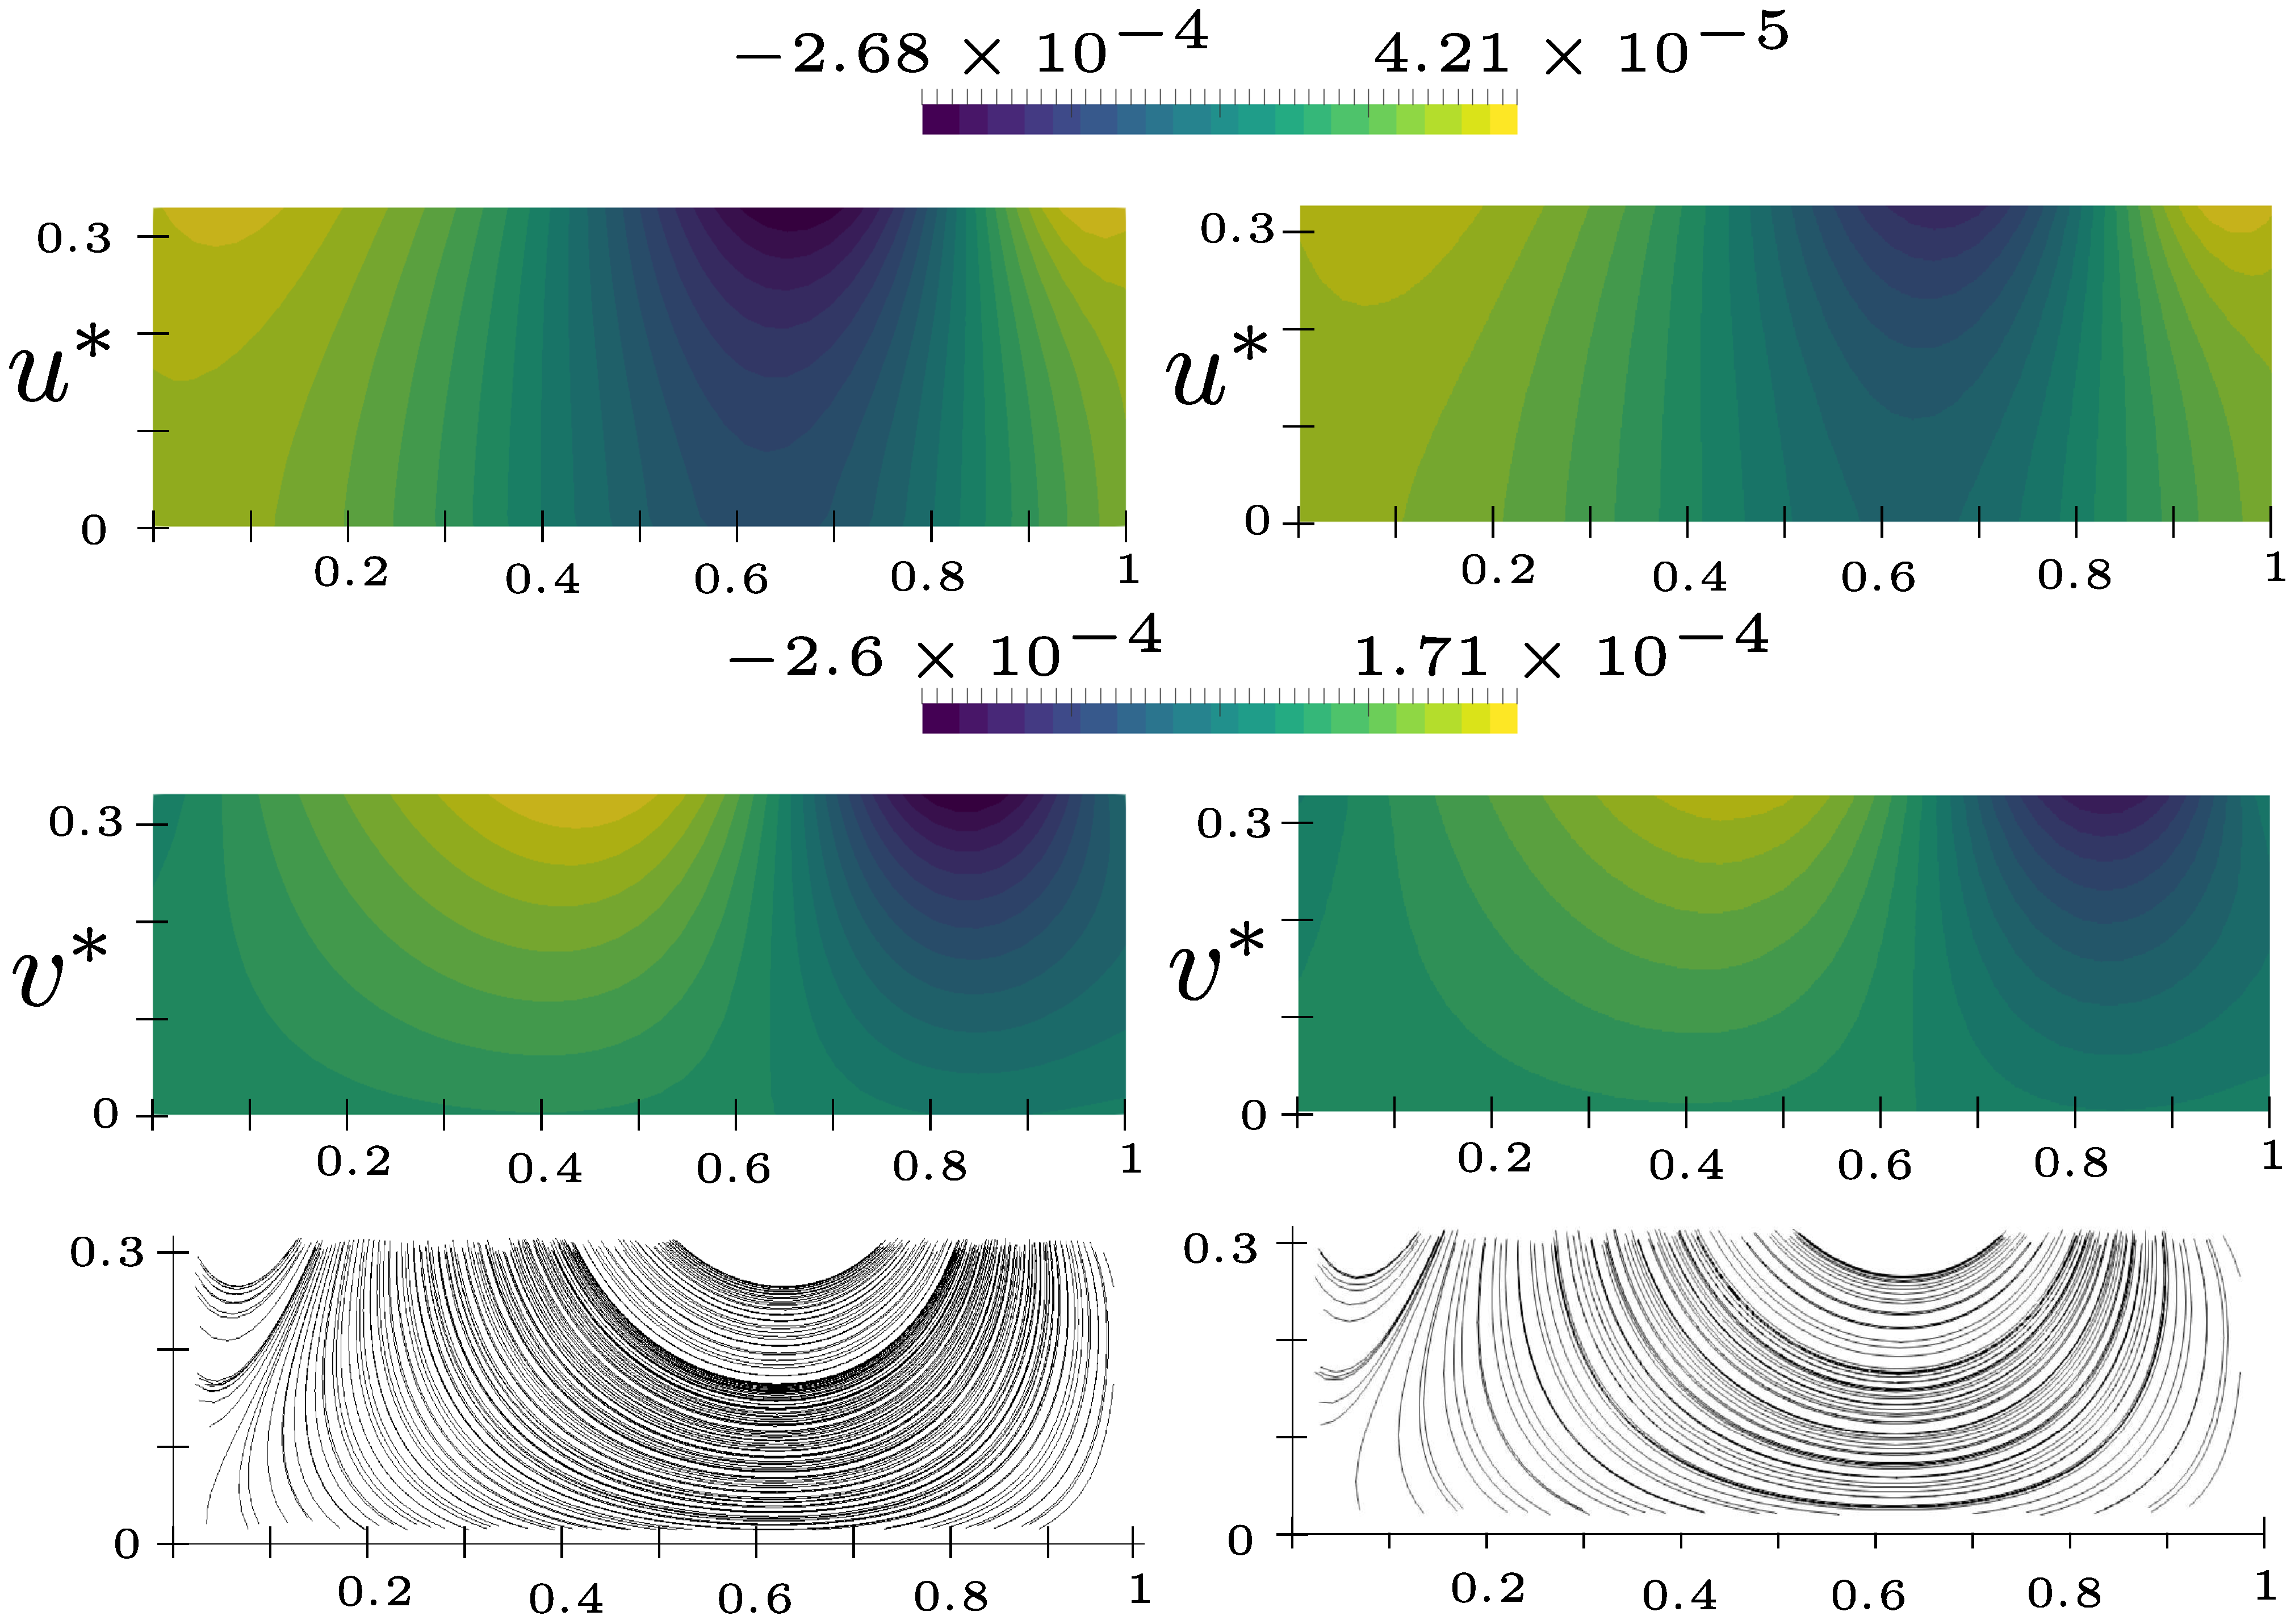
\includegraphics[width=1\linewidth]{chapter_5/figure/re100/vans_u}
	\caption{Left: VANS approach. Right: Homogenized DNS approach. The figure show, from top to bottom, the horizontal velocity the vertical velocity and the streamlines inside the porous domain $\Omega_p$}
	\label{fig:100_u}
\end{figure}

The DNS approach is used as reference case for the comparison. At Reynolds number equal to $100$ we have a fair agreement in the velocities and pressure gradients fields. The contours and the location of the local minima and maxima are the same for the two approaches. If we look at the numerical values, for some fields the relative errors are not negligible however, they are in mean always below $10\%$. Also the flow path inside the porous domain is in good agreement with the DNS data.
Some differences between the two models has to expected since in the VANS approach the micro-scale flow behavior is modeled. This means that some of the details that the full DNS is able to retain, are lost in the macroscopic approach. 

\begin{figure}[H]
	\centering
	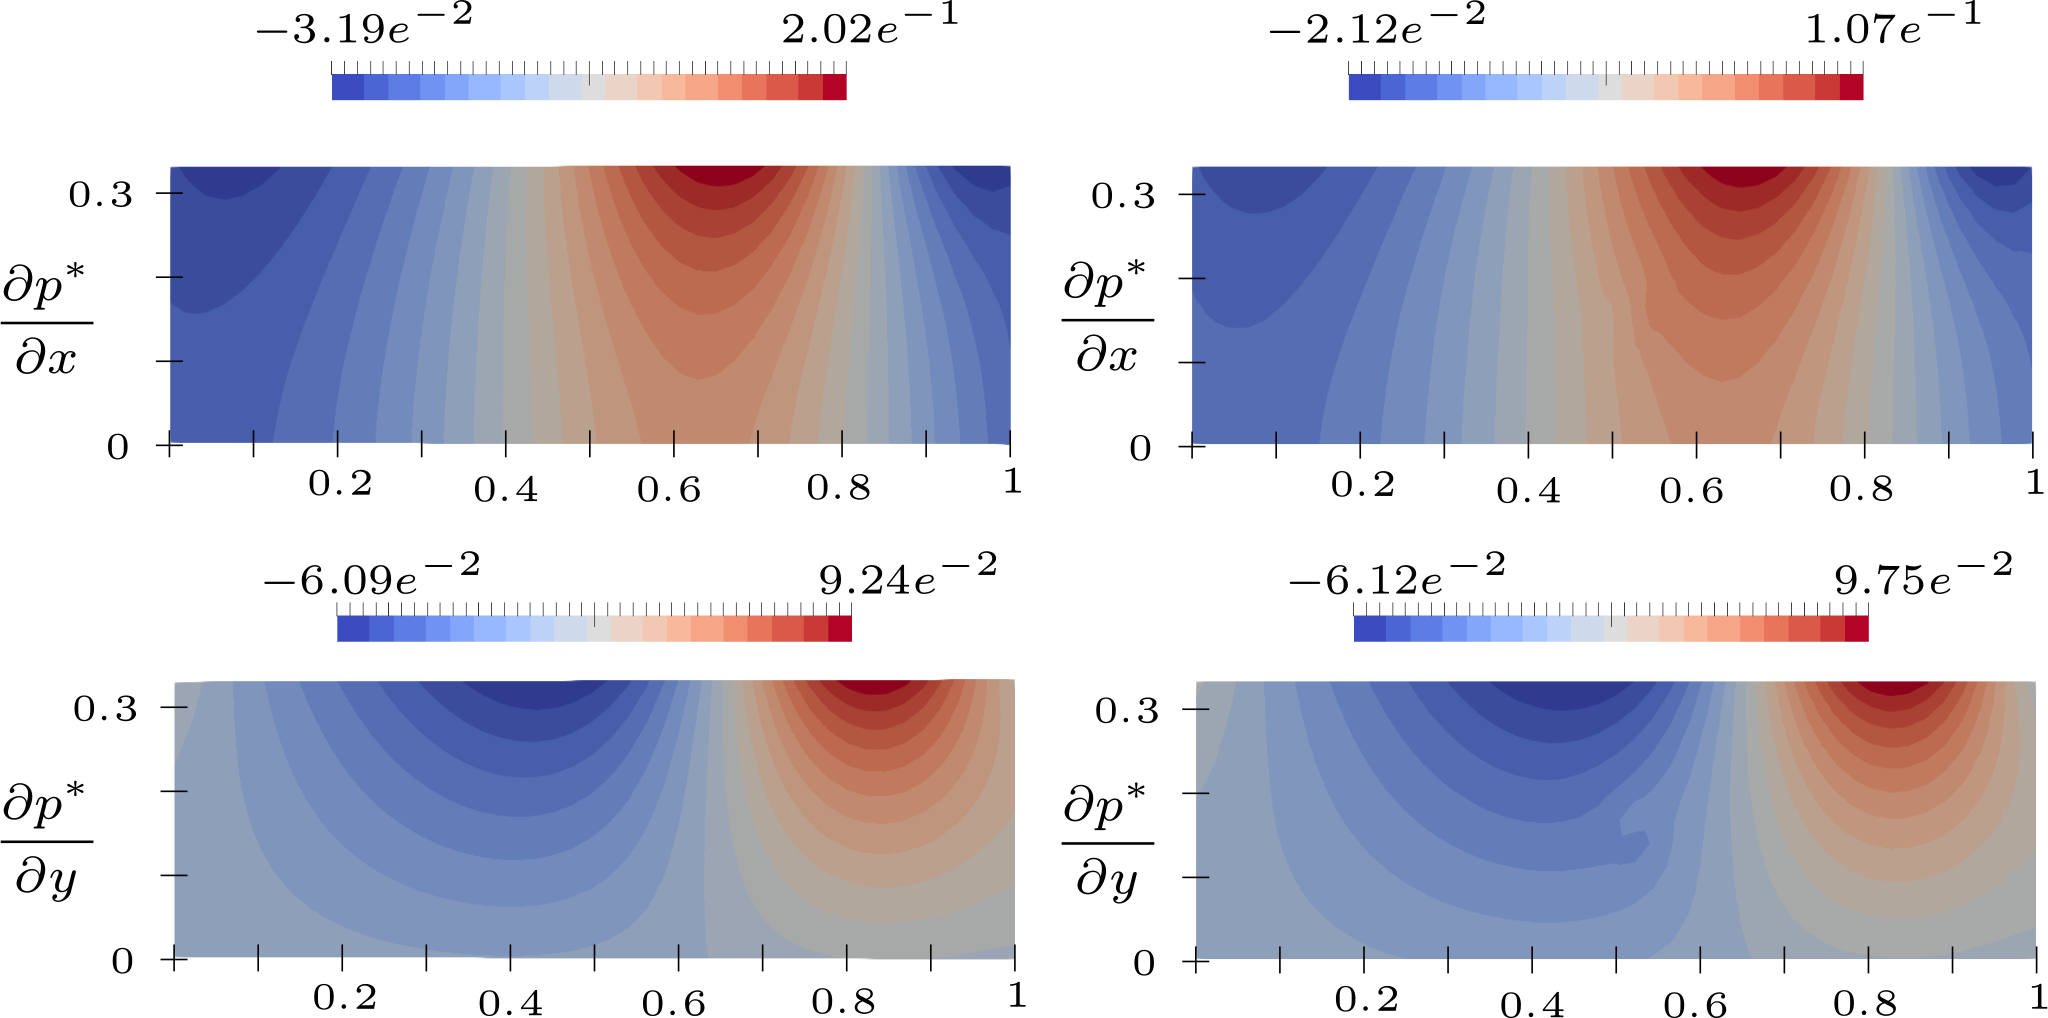
\includegraphics[width=1\linewidth]{chapter_5/figure/re100/vans_p}
	\caption{Left: VANS approach. Right: Homogenized DNS approach. The figure show, from top to bottom, the horizontal and the vertical component of the pressure gradient inside the porous domain $\Omega_p$}
	\label{fig:100_p}
\end{figure}


\subsection{Cavity $Re=1000$ comparison}

The same case and comparison has been done also for a Reynolds number equal to $Re=1000$.
For this case the same conclusion as the previous case are confirmed. Some of the relative errors are even smaller compared to the previous Reynolds number case. This support the robustness of our model in this range of Reynolds number.
These two solutions of the cavity problem shown that varying the permeability in a linear manner through the interface is the correct choice when using the penalization method.

\begin{figure}[H]
	\centering
	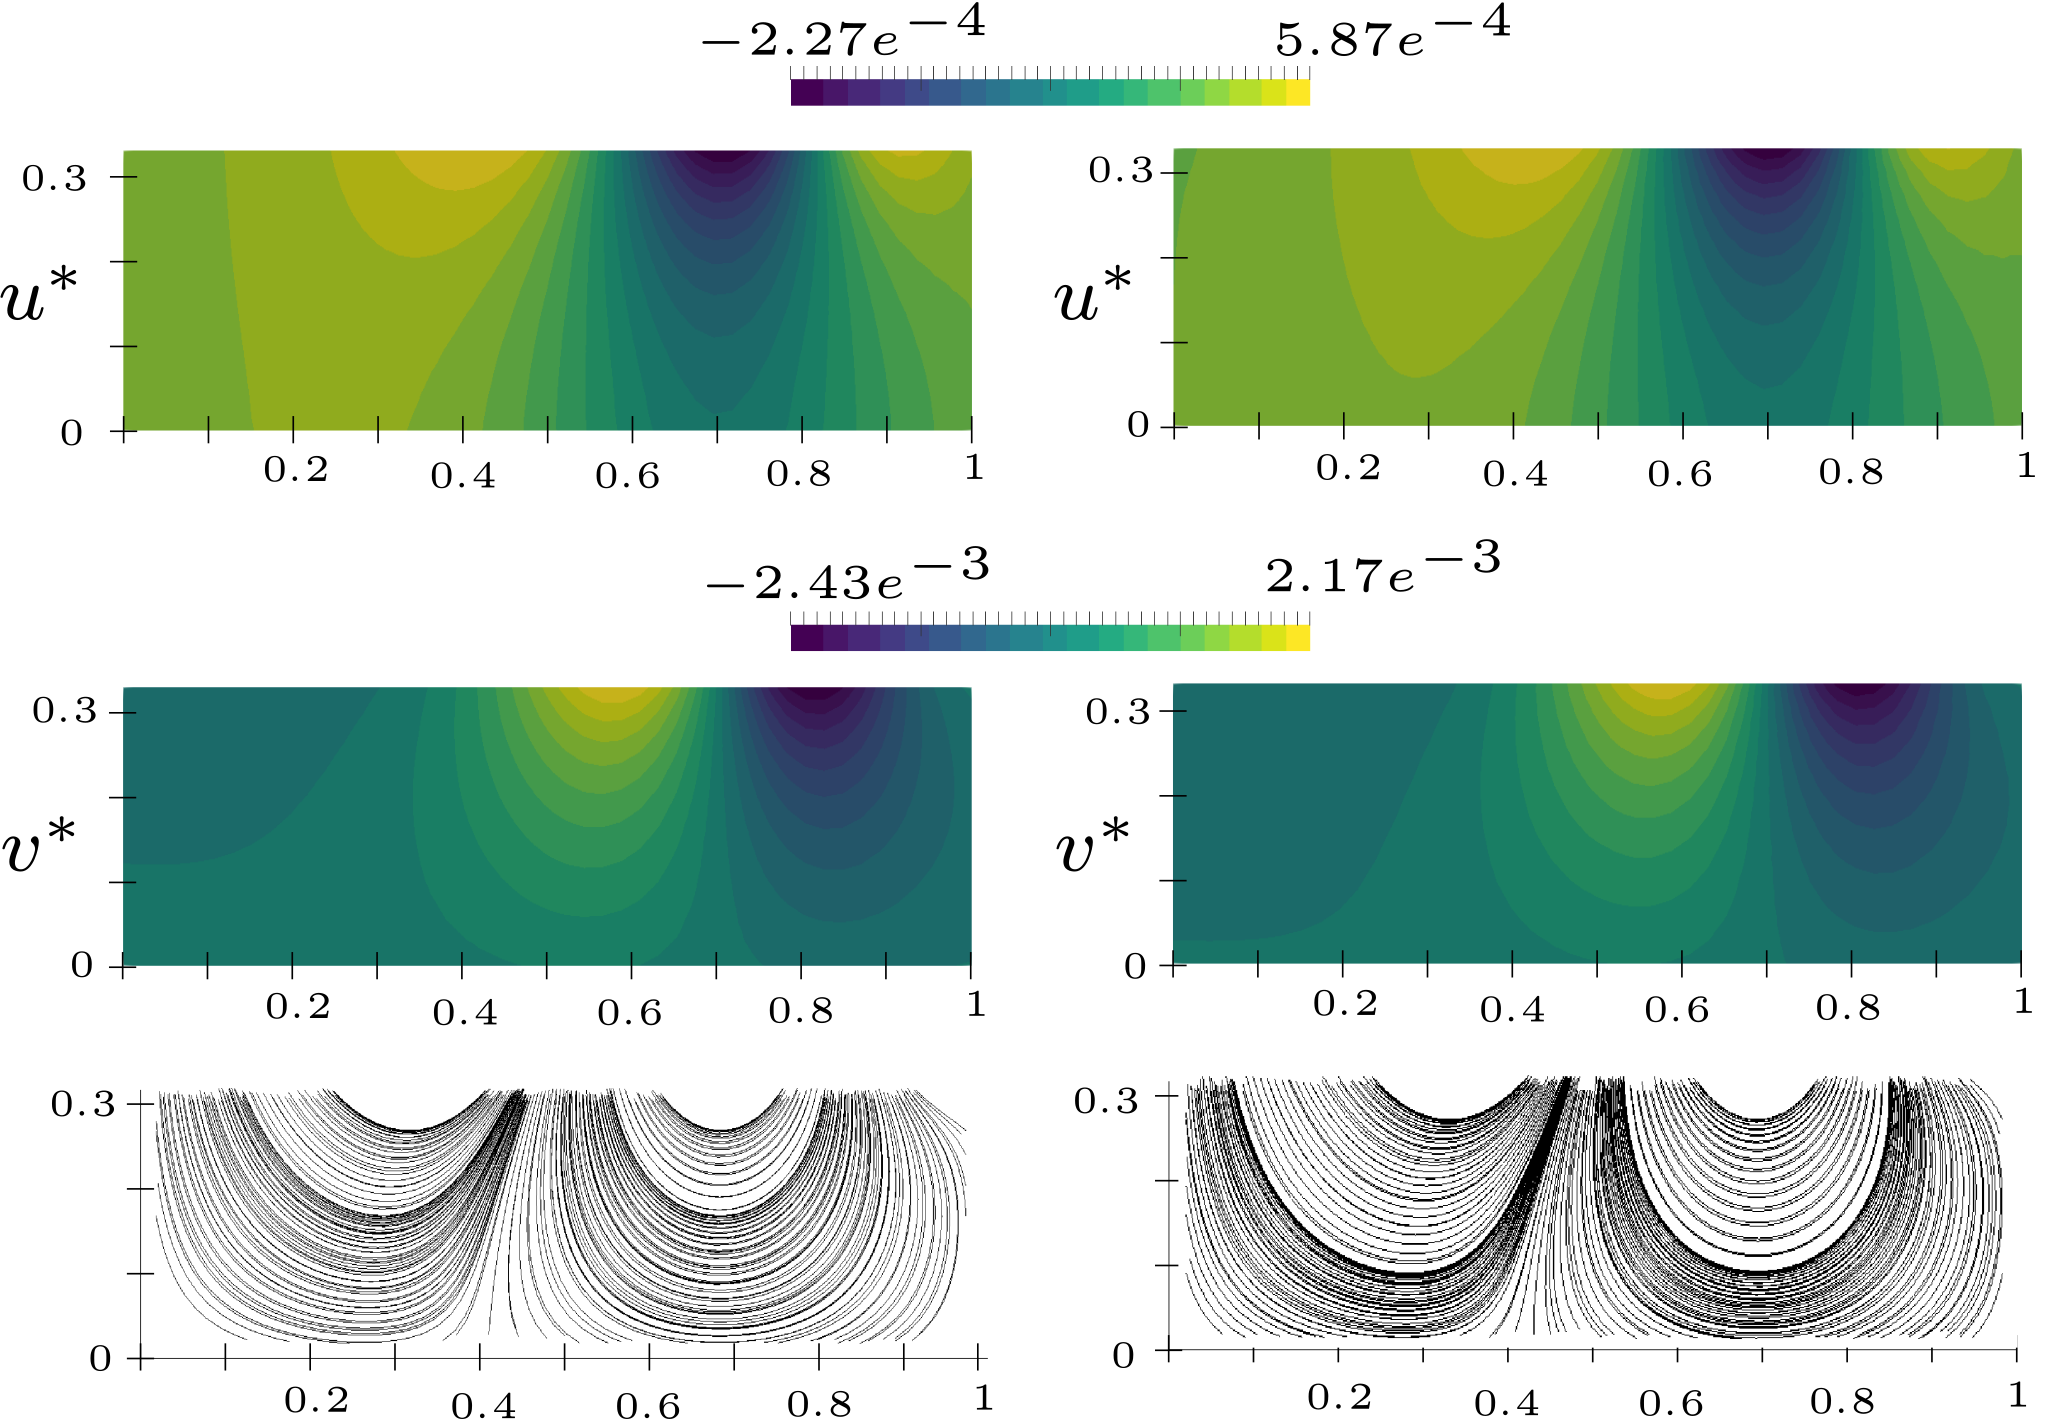
\includegraphics[width=1\linewidth]{chapter_5/figure/re1000/vans_u}
	\caption{Left: VANS approach. Right: Homogenized DNS approach. The figure show, from top to bottom, the horizontal velocity the vertical velocity and the streamlines inside the porous domain $\Omega_p$}
	\label{fig:1000_u}
\end{figure}

\begin{figure}[H]
	\centering
	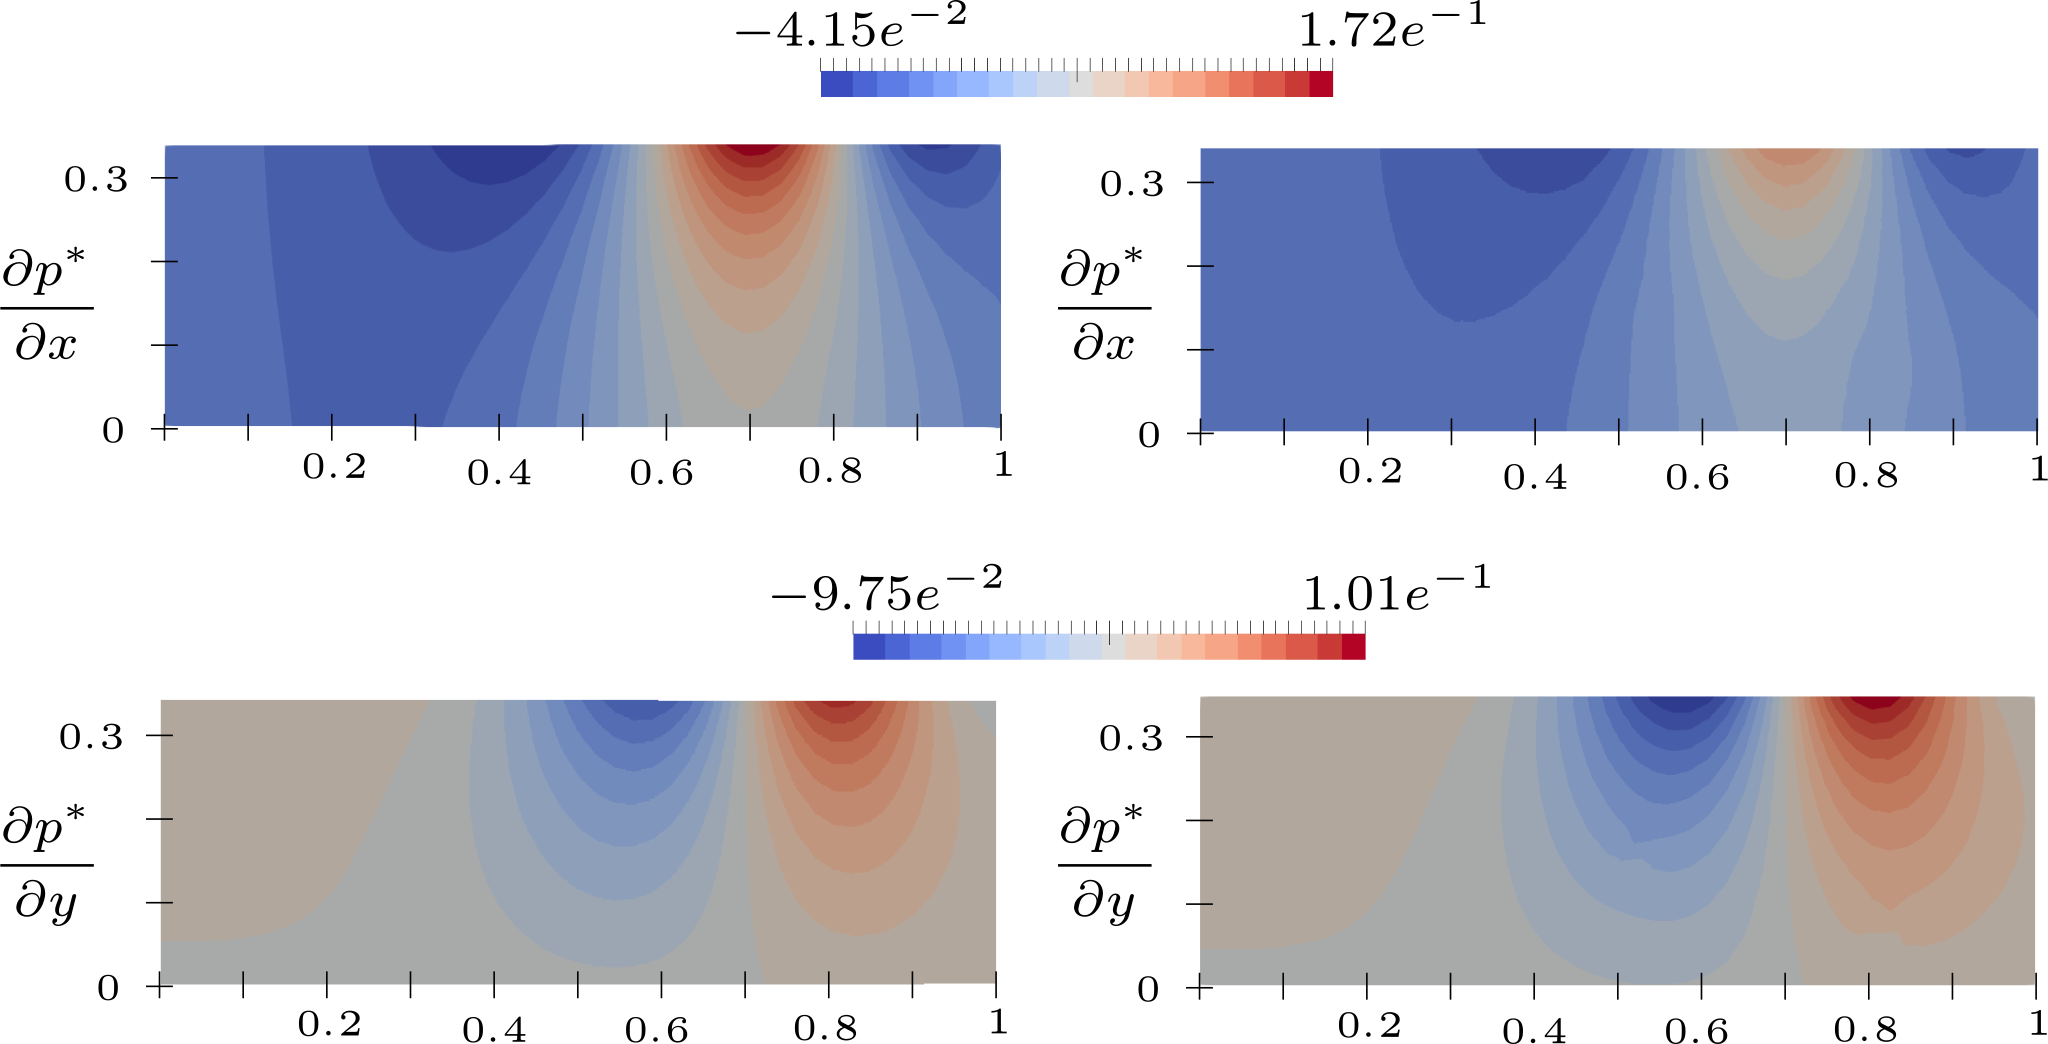
\includegraphics[width=1\linewidth]{chapter_5/figure/re1000/vans_p}
	\caption{Left: VANS approach. Right: Homogenized DNS approach. The figure show, from top to bottom, the horizontal and the vertical component of the pressure gradient inside the porous domain $\Omega_p$}
	\label{fig:1000_p}
\end{figure}


\subsection{Cavity $Re=5000$ using $\mathbf{H}$ metamodel}
\label{pr:mata_cav}
In our previous simulations the metamodel for the effective permeability has not been applied.  As a matter of fact the metamodel in chapter \ref{ch:4} was built for a porous medium made of staggered cylinders. So it would not be applicable when the porous medium is made by regular arranged cylinders.

In order to test how the effective permeability variability would impact our model we show the solution for another test case. In the same cavity geometry as before the system \eqref{eq:vans_cav} is solved with or without the Kriging metamodel for the effective permeability.

Although we have seen that at low pore Reynolds number the effective permeability is practically not sensitive in variation of flow direction and/or magnitude \footnote{see figures \ref{fig:08_H}, \ref{fig:08_H} and \ref{fig:08_H} in chapter \ref{ch:4}}.
For this reason also the Reynolds number has been increased to $5000$, that is still in the stationary regime but is near the transition limit (\citet{peng2003transition} ).

\begin{figure}[h]
	\centering
	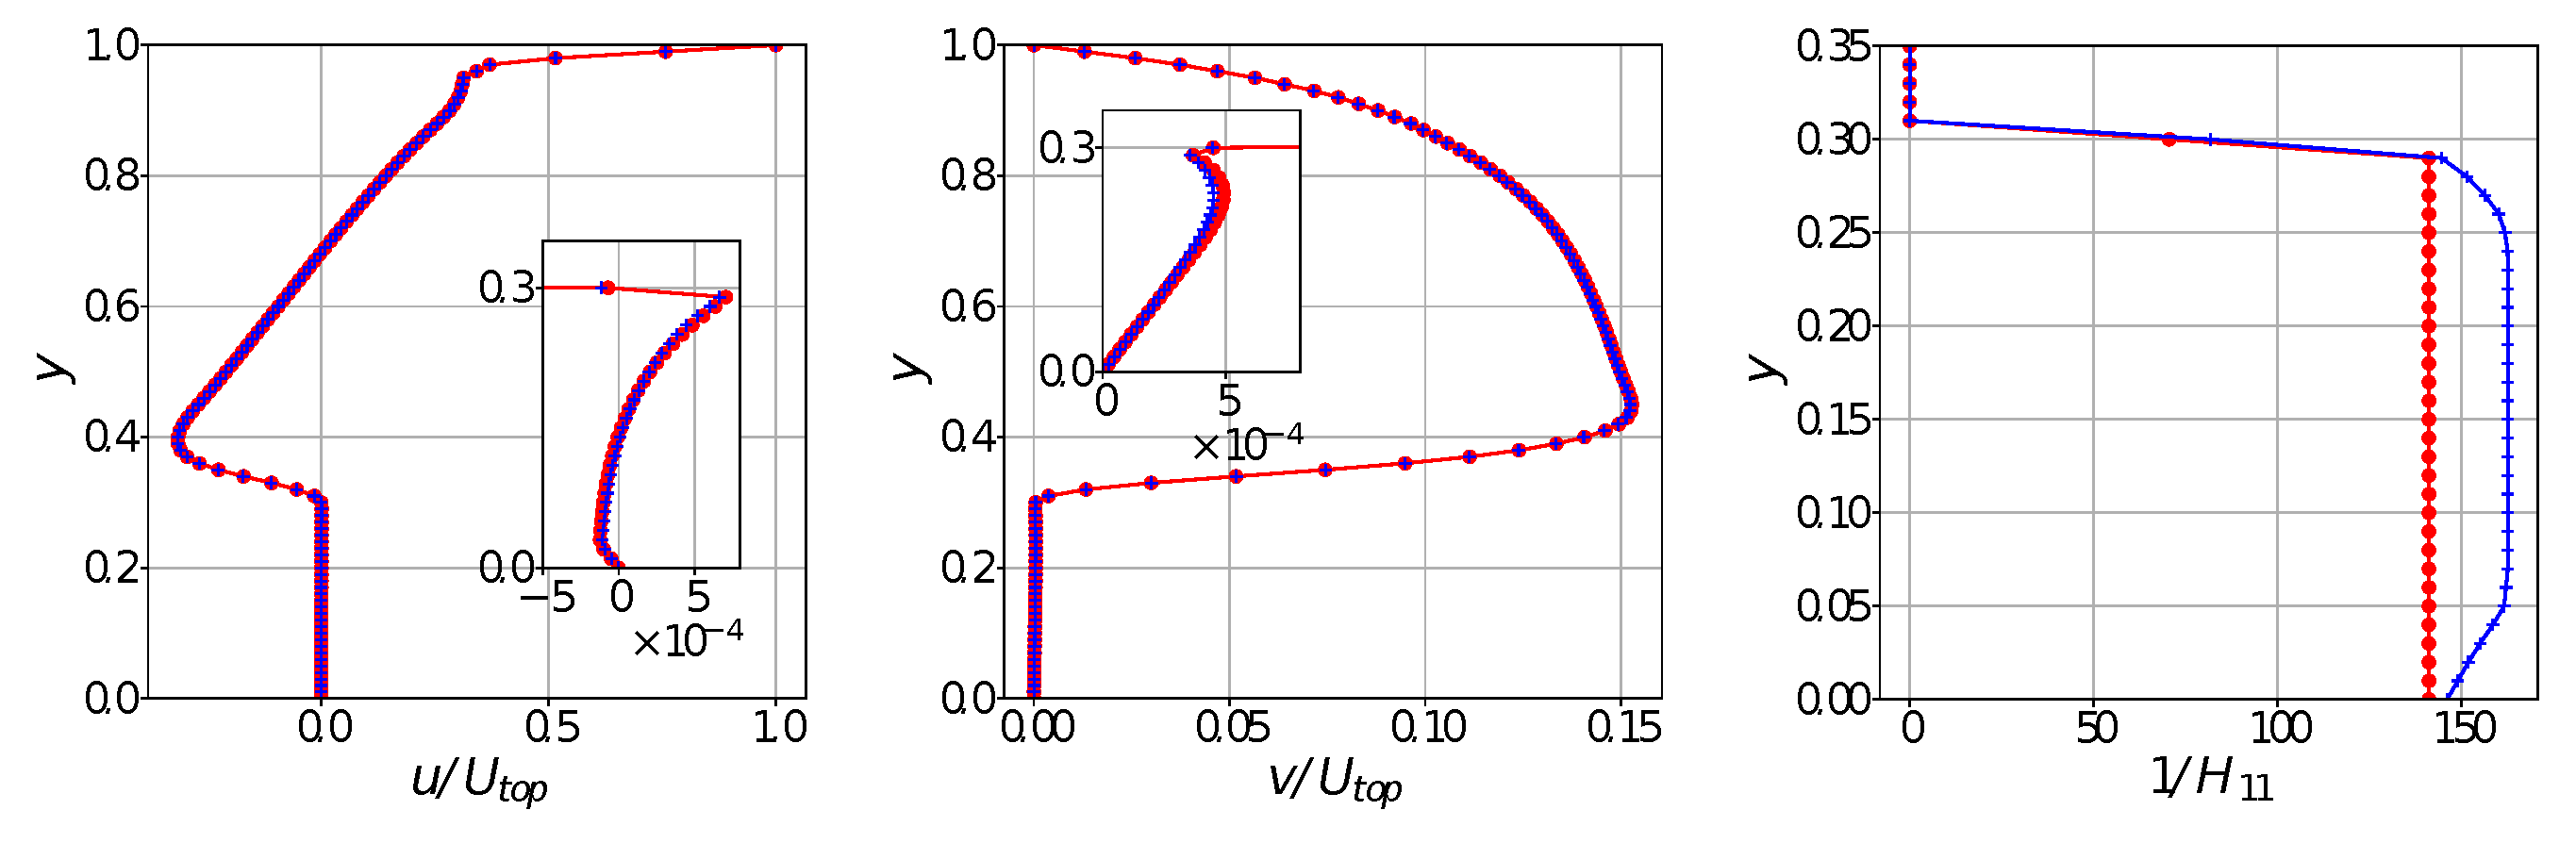
\includegraphics[width=0.9\linewidth]{chapter_5/figure/cav_5000}
	\caption{Left: horizontal velocity component. Center: vertical velocity component. Right: Effective permeability component $11$ . The three fields has been sampled at the center of the cavity geometry, $x_1=0.5 \,L$. The blue line represent the solution for the system \eqref{eq:vans_cav} with the Kriging metamodel for the effective permeability, the read line is the solution wo the same system with the model switched off.}
	\label{fig:cav5000}
\end{figure}

Figure shows \ref{fig:cav5000} the velocity and permeability profiles for a sample cut made at the center of the cavity at $x=0.5\,L$.
It is clear that the macroscopic velocity is not affected by the different treatment of the permeability, as a matter of fact the two velocities can be superposed almost precisely.
Although the inverse of the effective permeability component show some differences. At the interface the is possible to see also how the trend of the two different treatment look like the same at the interface. Although the permeability start to increase at a deeper vertical position then the case without metamodel. This is caused by the vertical angle $phi$ that is near to $90^\circ$ at that point because of the fluid penetration. The analysis made in chapter 4 shows that the permeability increase when the angle $\phi$ increase.
However the value of the permeability deep in the medium is almost the same. 
In any case even if there are some differences in the permeability profiles this seems not to effect the averaged velocities.

The fact that with the Kriging metamodel the same linear profile as equation \ref{eq:permeability_fun} is retrieved is another confirmation that the linear variation is the right choice.

%\footnote{The dots in the figure \ref{fig:cav5000} lines are used only to ease the read of the plots and do not correspond at the mesh nodes (that are too much to be represented clearly).}

\section{Separated flow between hills}
In chapter 1 we have presented some flow examples where a porous media layer in the leeward side of a bluff body can reduce the separation extension. In order to test the effectiveness of our model, to make prediction in this sense, the flow over periodically arranged hills has been chosen as test problem. This configuration has been already investigated experimentally and numerically and is a classical CFD bencmark problem now standardized by the ERCOFTAC committee.
It is used as a benchmark case to investigate the ability of DNS, RANS and LES models to resolve separation from a curved geometry.
The flow field features a large separation bubble caused by the curved surface of the hill and a natural reattachment in the flat part between the two hills crests. 
The flow is assumed to be periodic and two dimensional, at the Reynolds number tested. Numerous DNS and LES works can be found in literature with Reynolds numbers up to 10000 (\citet{chang2014simulations}, \citet{breuer2005issues}, \citet{breuer2009flow}, \cite{almeida1993wake} and \cite{temmerman2001large}).
This test case has been studied with two main objectives, to test the modeling and simulation issue related to our VANS solver and the physical capacity to reproduce the flow field behavior. 
Our idea is to extend the hill profile with a porous media layer and assess how the separation bubble is modified by the layer presence.
In our case we have tested small Reynolds number in the laminar regime. Although the problem has been chosen especially for the possibility to future extend the study in higher Reynolds number since a lot of data can be found in literature to validate the result.

\subsubsection{Geometry and condition}
The geometry of the problem is depicted in figure \ref{fig:mesh_hill}. It is two dimensional since the Reynolds number considered is in the laminar regime and the flow do not present any three dimensional characteristic in this range. The dimension of the hill crest and extensions are also showed in the same pictures being non-dimensional with the hill crest height. The chosen dimensions of our setup are: $L_x = 9.0$, $L_y = 3.036$ and $h = 1$ where $x,y,z$ are the streamwise, wall-normal and spanwise direction, respectively. We solve the flow inside of a single streamwise periodic segment and thus covers solely one complete hill region from crest to crest.
Between one hill and the next one there is a flat plate region of extension $5h$. The pressure induced separation takes place from the first hill curved surface and reattachment is observed at the flat plate part between the two hills.

The hills profile is described by a polynomial parametric curve function of the streamwise direction $y_{hill} = f(x)$. The specific coefficients and definition can be found in \citet{almeida1993wake}. This geometry is also named \textbf{base} case in the following text.

The problem is discretized using the finite volume method implemented in OpenFoam and the mesh used is showed in figure \ref{fig:mesh_hill}. The mesh is purely made of hexahedral cell and counts 25000 elements in the two dimensional version. It is possible to download it at \url{https://turbmodels.larc.nasa.gov/Other_LES_Data/2dhill_periodic.html}. The resolution has been already validated in DNS and LES computations so it has not been further investigated here.

\begin{figure}[h]
	\centering
	\includegraphics[width=1\linewidth]{chapter_5/figure/mesh}
	\caption{Domain of the problem and mesh used to discretize it. On the right side there is an enlargement of the zone on the hill curvature.}
	\label{fig:mesh_hill}
\end{figure}

The inlet and the outlet patches are connected with a periodic boundary condition, at the hill and flat plate surface the no-slip condition is imposed and finally at the top of the domain a slip condition is used.
The numerical setup for the numerical scheme and linear solvers is the same as the DNS simulations in chapter 4 paragraph \ref{ph:numeric_setup}.

The equation solved are a slightly modified version of the VANS system \eqref{eq:vans_cav} in which the constant macroscopic pressure gradient is introduced as a source term in the momentum.
The non-periodic behavior of the pressure field can be accounted for by adding the mean pressure gradient as a source term to the momentum equation in streamwise direction.

\begin{eqnarray}
\begin{cases}
\derp{\vbms}{t} + \dfrac{1}{\varepsilon} \nabla \cdot \left[  \vbmi  \vbmi \right] = -\dfrac{1}{\rho_{\beta}} \nabla \meani{\pb} + \nub \nabla^2 \vbmi \\ 
\qquad \qquad \qquad \qquad \qquad \qquad- \nub \varepsilon \mathbf{H}^{-1} \vbmi +\dfrac{\nub}{\varepsilon} \nabla \varepsilon \cdot \nabla \vbmi + \dfrac{\nub}{\varepsilon} \vbmi \nabla^2 \varepsilon - \mathbf{g}\\
\nabla \cdot \left(\varepsilon \vbmi \right) = 0\\
\vbms = 0 \qquad \textrm{at hill wall} \\
\derp{u}{y}=0 \qquad \textrm{at} y = 3.035h\\
\vbms|_{x_1 = 0} = \vbms|_{x_1 = 9h} \\
\pbms|_{x_1 = 0} = \pbms|_{x_1 = 9h} 
\end{cases}
\label{eq:sys_hill}
\end{eqnarray}

In the system \eqref{eq:sys_hill} the flow is driven by the source term $\mathbf{g}$ and the Reynolds number is computed a posteriori in the following manner:
$$
R_e = \dfrac{U_b h}{\nu}
$$
where $U_b$ is the velocity in the top left corner of the domain, just above the first hill.

The treatment for the porosity is the same as equation \eqref{eq:porsitity_fun} where in this case the $y_{itf}$ is described by two different profiles.
The first one that is called \textbf{external} is the same hill profile translated to the right by a length equal to $0.2\,h$ in the streamwise direction. This setup is used to test the case of a porous media layer on the external part of the hill. In this case the hill geometry is modified.

In the second case the interface profile $y_{itf}$ is exactly the hill profile at the same position and the the solid part of the hill is translated in the direction $-x$ by $0.2\,h$. In this setup the porous media layer has been inserted on the "inside" of the hill leeward side. It means that the total the geometrical extension of the hill plus the porous media layer is the same as the base case described by $y_{hill}$.

The porous media layer has the same geometry of the one described in \ref{ch:4}, a series of cylinders in staggered arrangement. The cylinders are then arranged on the leeward side of the hill and they are aligned with the wall normal direction. Although their extension is not uniform, the line that pass through all the cylinders lid describe the curves $y_{itf}$ \textbf{external} and \textbf{internal}.

The two different porosity field arrangements are depicted in figure \ref{fig:por_gauss}. Where the porosity deep inside the medium, showed in green, is equal to $0.8$ and the exterior porosity field is equal to $1$ and is showed purple.

\begin{figure}[h]
	\centering
	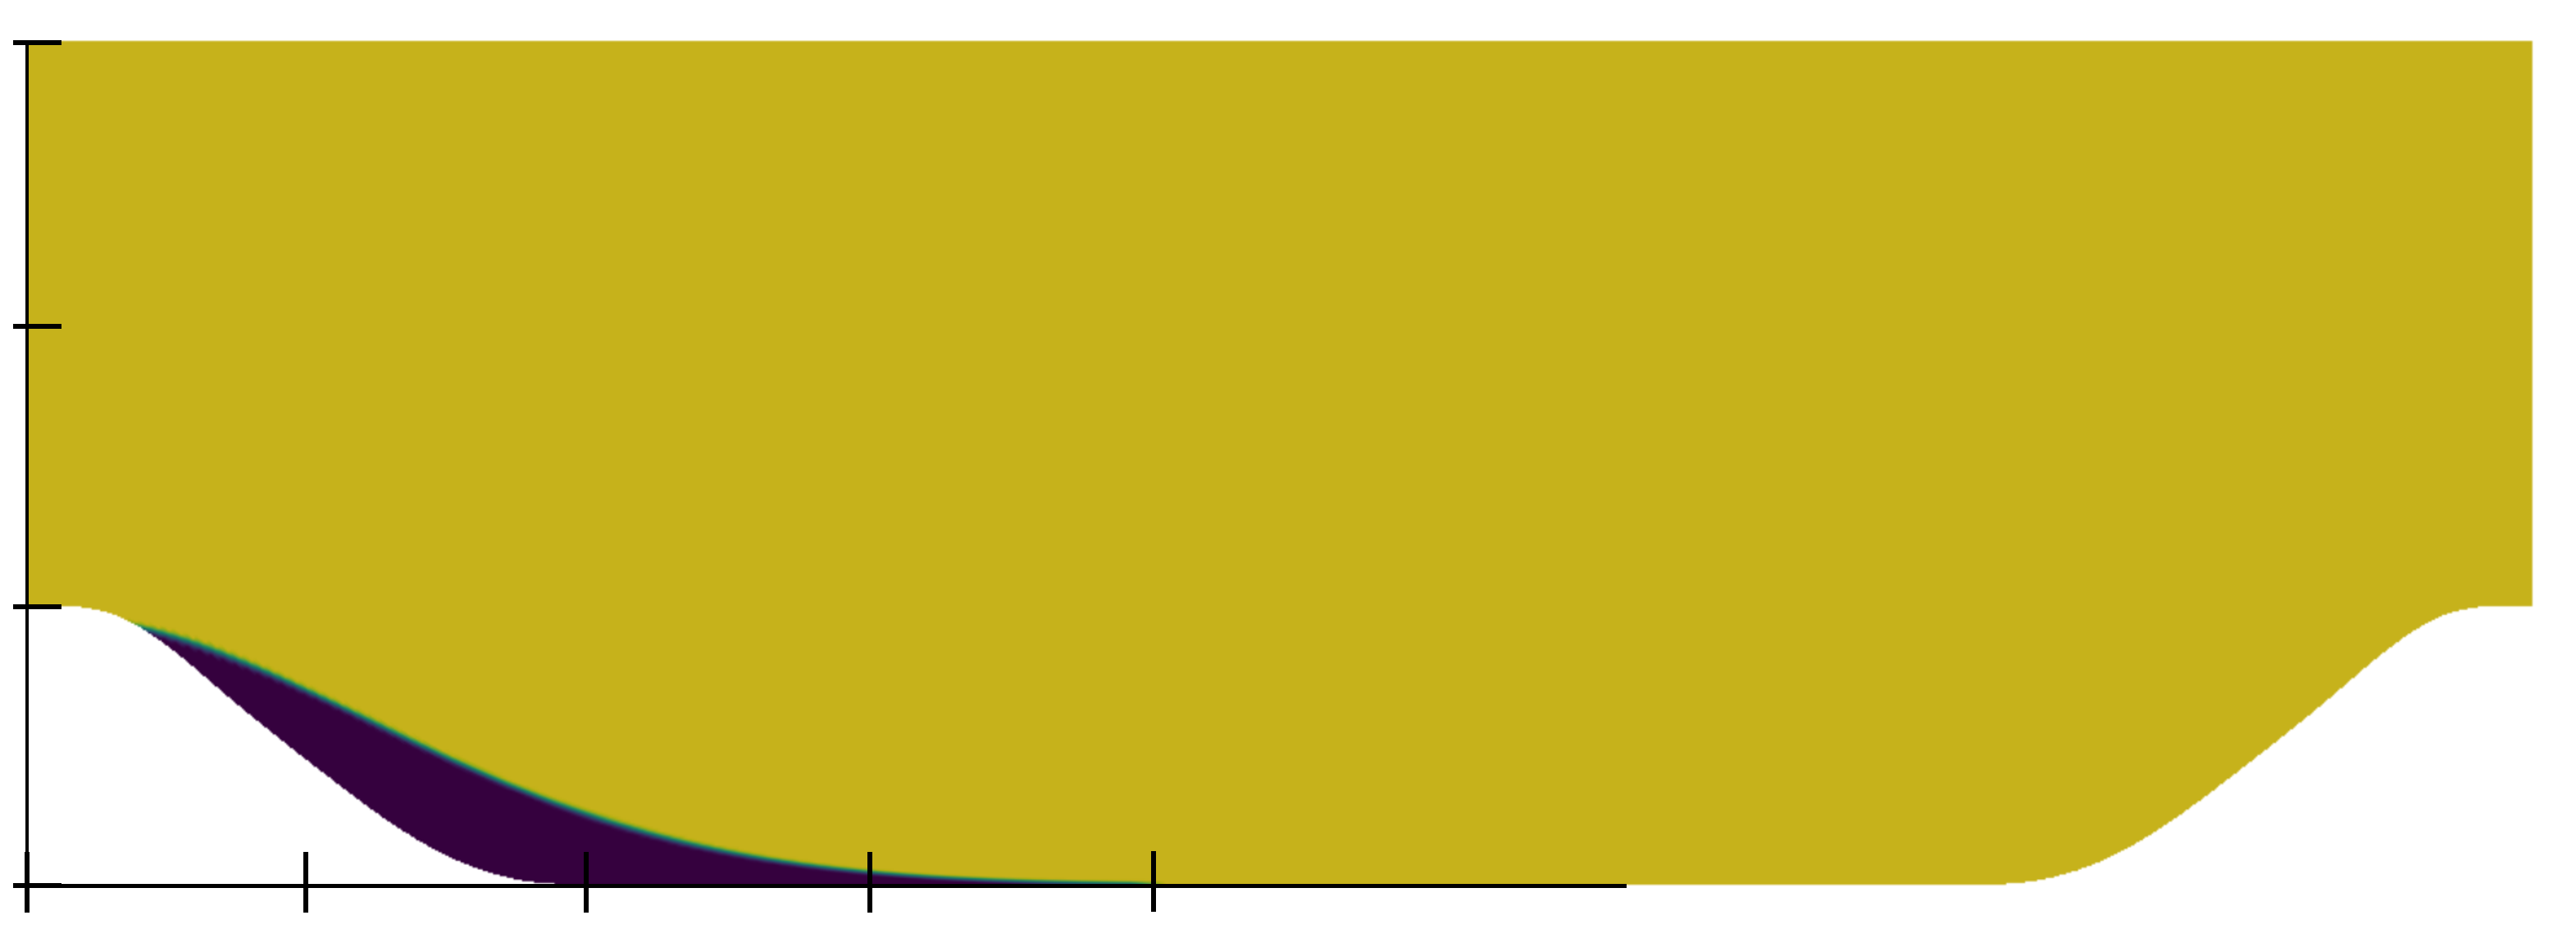
\includegraphics[width=1\linewidth]{chapter_5/figure/por}
	\caption{Porosity field in the leeward side of the first hill for the two different cases \textit{external} and \textit{internal}. The porosity in the deep medium is equal to $0.8$ and is colored in green, instead the porosity in the free fluid is equal to $1$ and it is colored in purple. On the left case, the \textit{external} one, the red line describe the hill profile of the base case and the white line describe the porous media interface. For the \textit{internal} case on the right the base hill profile and the porous media interface are the same one, and they are depicted in white.}
	\label{fig:por_gauss}
\end{figure}

On figure \ref{fig:por_gauss} the left picture shows the case named \textit{external}, the red line indicate the hill profile in the base case and the porous media layer is put on top of it and the white line indicate the porous media interface $y_{itf}$.
The right picture in figure \ref{fig:por_gauss} instead show the configuration in the case named \textit{internal}. For this case the porous media interface line $y_{itf}$ is the same as the hill profile in the base case and is depicted in white.

To summaries the two different cases differ for the position on the porous media interface that is equal to the hill profile translated in the positive streamwise direction (case \textit{external}) of in the negative streamwise direction (case \textit{internal}). The translation has the same extension of $0.2\,h$ for each case.

The interface has also been treated with the linear smoothing function \eqref{eq:porsitity_fun}.

The permeability tensor components are then evaluated with the Kriging metamodel in the zone where the porosity field is different from one. That describe indeed the porous domain.


\subsection{Comparison between smooth and porous leeward side of the hill}

The above geometrical setup has been studied in the stable laminar regime. In this case the source term is equal to $\mathbf{g} = (0.5e^{-9} \quad0 \quad0)$ that results in a Reynolds number equal to $83$.
For all the cases the recirculation bubble has been measured in his vertical and horizontal extension. The horizontal extension $L_R$ is defined as the first streamwise point in which a sampled velocity profile shows only positive streamwise velocities. The vertical extension has been measured at $x=4.5$ that is the mean extension of the domain.
Table \ref{tb:bubble} collect these results. Looking at the results the porous media has a negative effect either in $L_R$ and $h_{x=4.5}$. For the case \textit{external} the geometry of the hill is modified indeed by the porous medium and the leeward side is pushed downstream, so is not surprising that the recirculation extension is pushed downstream itself. Although the same negative effects can be found also for the \textit{internal}. This is line with some observation made by \citet{jimenez2001turbulent} and \citet{segura2017permeable} in which they arguments that some configuration of the porous surfaces characteristic (porosity and permeability) can produce negatives effects.

\begin{table}[h]
	\centering
	\begin{tabular}{c|c|c}
		case & $L_R$ & $h_{x=4.5}$ \\ 
		\hline 
		\hline 
		\textit{base} & 5.6 & 0.27 \\ 
		\hline 
		\textit{external} & 5.95 & 0.33 \\ 
		\hline 
		\textit{internal} & 5.8 & 0.31 \\ 
		\hline 
		\hline 
	\end{tabular}
	\caption{Recirculation bubble streamwise extension $L_R$ and vertical extension at $x=4.5$ for the three porous media configuration.}
	\label{tb:bubble}
\end{table}

The streamlines in figure \ref{fig:streamlines} show the shape of the recirculation bubble for the three cases. It can be seen that they look very similar and as a matter of fact the differences described in table \ref{tb:bubble} are around the $5\%$ of difference from the base case without the porous layer.
In figure \ref{fig:cuts_hill} the local velocity fields are analyzed. The sampled velocities at $x=1$ seems very different because the geometry in that point is not the same. Although if we look at the horizontal velocity gradients are similar. Some differences can be shown for the vertical velocities. The \textit{internal} case present smaller vertical velocities than the other two cases at $x=1$ so close to the detachment point. The situation is inverted further downstream at $x=2$ and the three profiles collapse one into another at $x=3$. This different local behaviors can be used for example in situations were the vertical exchange of momentum has to enhanced for examples in aquatics plant applications where the nutrient exchange has to be optimized.

\begin{figure}[H]
	\centering
	\includegraphics[width=1\linewidth]{chapter_5/figure/streamlines}
	\caption{Streamlines for the three cases tested. The top picture show the case without the porous medium. The central picture show the case where the porous media layer is put on the external part of the leeward side and the bottom case show the case with porous medium put inside the leeward side.}
	\label{fig:streamlines}
\end{figure}


\begin{figure}[H]
	\centering
	\includegraphics[width=1\linewidth]{chapter_5/figure/cuts_hill}
	\caption{The top three figures show the horizontal velocity profile for the sampled cut at $x=1$, $x=2$ and $x=3$ respectively from left to right. The bottom figures follow the same patterns but instead shows the vertical velocity profile. The red line is the \textbf{base} case the blue line is the \textbf{external case} and the green line is the \textbf{internal} case.}
	\label{fig:cuts_hill}
\end{figure}


\section{Conclusions}

In the chapter we have shown how the VANS equations derived in chapter 2 can be used to describe the averaged macroscopic field for rigid porous medium. We have also shown how the interface should be threated in order to retrieve good results. Direct comparison with DNS data show that the linear smoothing of either the porosity filed and the effective permeability filed are necessary. We have also shown that using the metamodel developed for $\mathbf{H}$ produce the same smoothing for the interface. Finally the periodic hill application show that our homogenized solver can be used easily as a tool to test and measure porous coating and their effectiveness.
For the porous characteristic used in our test we have found that the porous medium has negative effects for separation. But our focus were posed on the validation of the correctness and easiness to use of our macroscopic model. With this tool is now possible to extensively study this porous media coating in order to find the optimal characteristics for different objectives.
%If it would be possible to obtain systematically the same results with a reduced information model \footnote{like a general metamodel or a macroscopic model for porous media or a turbulence model for turbulent flow} and a full physic simulation we would be in a paradox. Basically it would means that some of the input information are redundant. This statements should be kept in mind when making analysis on the macroscopic model against the DNS.

\chapter{Conclusions and recommendation}


bla bla...

\Red{write clearly that you have taken Reynolds 100 max because after that the closure problems are not true. In fact the linear correlation hypothesis holds till 100. The check has been performed comparing H from inverting the DNS field and Darcy relation and the H from the closure problems, or comparing the latter  directly with the force}

\subsubsection{Possible future extensions}

bla bla...
\chapter*{Appendix A: Kriging metamodel}

The Kriging metamodel has already been briefly introduced in chapter \ref{ch:4} but here we want to talk a little bit more on the numerical procedure behind it and also present some implementation example.

The Kriging method was first aimed to make prediction of missing geostatics data (\citet{krige1951statistical}). However this methodology has been further generalized and applied extensively in recent literature as metamodel for large variety of experiments.
The method can treat highly non linear output and can be used to either interpolate or extrapolate response from a sample design set.

In this discussion the $\hat{f}(\boldsymbol{\chi})$ is a model for the function $f(\boldsymbol{\chi})$ and $\hat{y}$ is the model prediction of the true response $y = f(\boldsymbol{\chi})$ that is evaluated at the point $\chi$. $n$ is the number of point in the sample design set and $k$ is the number of input of the experiment.

After the exploration of the design possibilities the database produced is usually organized as $(\mathbf{x_i}, y(\mathbf{x_i}))$  $i=1,...,n$ where
\begin{itemize}
	\item $\mathbf{x_i}$ is the i-th vector element containing the $k$ input parameters for the i-th experiment run
	\item $y_i$ is the scalar response of the experiment for the vector of inputs $\mathbf{x_i}$ \footnote{$y_i$ is always a scalar because even in case of multiple output for an experiment run they are supposed to be uncorrelated. It means that if we had $p$ elements in each $\mathbf{y_i}$ will have to build $p$ metamodels}
\end{itemize}
Also the $n \times k$ matrix containing all the inputs is indicated with $\mathbf{X}$ and the $n \times 1$ vector containing all the responses is indicated as $\mathbf{Y}$

The Kriging response for a new untried input point $\boldsymbol{\chi}$, containing $k$ elements, is given by the linear \textit{predictor}:
\begin{equation}
\hat{y} = \hat{f}(\boldsymbol{\chi}) = \sum_{i=1}^{N} \lambda_i(\mathbf{x}) f(\mathbf{x_i}) =  \sum_{i=1}^{N} \lambda_i(\mathbf{x}) y_i
\end{equation}

$\hat{y}$ is considered to be a new realization of the random Gaussian process that has generated the set of responses $\mathbf{Y}$.
The weights $\lambda_i$ are the solution of a linear system obtained by minimizing the variance of the error between the predictor and the random process.
The best \textit{linear unbiased predictor} BLUP is so obtained finding the weights $\lambda_i$ that minimize:

\begin{equation}
MSE[\hat{y}(\chi)] =  E \left[\left( \hat{f}(\boldsymbol{\chi})  -f(\boldsymbol{\chi}) \right)^2\right] = E \left[\left(\lambda(\chi)\mathbf{Y} -y(\chi)\right)^2\right]
\label{eq:var_err}
\end{equation}

under the unbiasedness condition:

\begin{equation}
E \left[ \hat{f}(\chi)  -f(\chi)\right] =  E \left[ \boldsymbol{\lambda}(\boldsymbol{\chi})\mathbf{Y} -\mathbf{y}(\boldsymbol{\chi})  \right] = 0
\label{eq:unb_cond}
\end{equation}
this relation means that the predictor and the Gaussian process have the same mean value for every new point $\boldsymbol{\chi}$.

The equation \eqref{eq:unb_cond} is further developed yielding:
\begin{equation}
E \left[ \hat{f}(\chi)  -f(\chi)\right] = \boldsymbol{\lambda} E \left[ f(\mathbf{X})  \right] - E \left[ f(\boldsymbol{\chi})  \right] = \sum_{i=1}^{n} \lambda_i(\boldsymbol{\chi}) \mu(\mathbf{x_i}) - \mu(\boldsymbol{\chi}) = 0
\label{eq:unb_cond2}
\end{equation}
where $\mu(\boldsymbol{\chi})$ is the mean value of the true function at the point $\chi$, instead $\mu(\mathbf{x_i})$ is the mean of all the realizations collected for the database.

Different type of Kriging approximation exist accordingly on how $\mu(\boldsymbol{\chi})$ is evaluated:
\begin{itemize}
	\item \textit{simple Kriging} assume that the trend has null value: $\mu(\boldsymbol{\chi}) = 0$
	\item \textit{ordinary Kriging} assume that the trend is an unknown constant: $\mu(\boldsymbol{\chi}) = \mu$
	\item \textit{universal Kriging} assume that the trend is the solution of a generalized \textit{least squares model} in which is possible to decide the order ($n_{\beta}$) \footnote{It means that, for example, taking $n_{\beta}= 2$ the least squared model is quadratic} of the chosen base: $\mu(\boldsymbol{\chi}) = \mathbf{g}(\boldsymbol{\chi})^T \boldsymbol{\beta}$
	Where $\mathbf{g}(\boldsymbol{\chi})$ is the base evaluation at the point $\boldsymbol{\chi}$ and the vector $\boldsymbol{\beta}$ contains the $n_{\beta}$ coefficients of the model.
\end{itemize}

The unbiased condition \eqref{eq:unb_cond2} can be so rewritten, without loss of generality, as:
\begin{eqnarray}
	&& \boldsymbol{ \lambda} (\boldsymbol{\chi}) \mathbf{G}(\mathbf{X}) \boldsymbol{\beta} - \mathbf{g}(\boldsymbol{\chi}) \boldsymbol{\beta} = 0 \nonumber \\
	&& \boldsymbol{\lambda}(\boldsymbol{\chi}) \mathbf{G}(\mathbf{X}) = \mathbf{g}(\boldsymbol{\chi})
\end{eqnarray}
where $\mathbf{G}(\mathbf{X})$ is the $n \times n_{\beta}$ matrix containing the evaluation of the least squared basis functions at all points in $\mathbf{X}$

Also the relation \eqref{eq:var_err} can be manipulated:
\begin{eqnarray}
E \left[\left( \hat{f}(\boldsymbol{\chi})  -f(\boldsymbol{\chi}) \right)^2\right] &=& var(  \hat{f}(\boldsymbol{\chi})  -f(\boldsymbol{\chi}) ) \nonumber \\
&=& var(\hat{f}(\boldsymbol{\chi}))  +var(f(\boldsymbol{\chi})) -2 \; cov( \hat{f}(\boldsymbol{\chi}),f(\boldsymbol{\chi})) \nonumber \\
&=& var( \sum_{i=1}^{n}\lambda_i(\boldsymbol{\chi}) f(\mathbf{x_i}) )  +var(f(\boldsymbol{\chi})) -2 \; cov( \sum_{i=1}^{n}\lambda_i(\boldsymbol{\chi}) f(\mathbf{x_i}),f(\boldsymbol{\chi})) \nonumber \\
&=&  \sum_{i=1}^{n} \sum_{j=1}^{n} \lambda_i(\boldsymbol{\chi})\lambda_j(\boldsymbol{\chi}) cov(f(\mathbf{x_i}),   f(\mathbf{x_j})) +var(f(\boldsymbol{\chi})) -2 \;  \sum_{i=1}^{n}\lambda_i(\boldsymbol{\chi}) cov(f(\mathbf{x_i}),f(\boldsymbol{\chi})) \nonumber \\
&=& \sum_{i=1}^{n} \sum_{j=1}^{n} \lambda_i(\boldsymbol{\chi})\lambda_j(\boldsymbol{\chi}) cov(\mathbf{x_i}, \mathbf{x_j}) +var(f(\boldsymbol{\chi})) -2 \;  \sum_{i=1}^{n}\lambda_i(\boldsymbol{\chi}) cov(\mathbf{x_i},\boldsymbol{\chi})
\label{eq:BLURP}
\end{eqnarray}
where $\mathbf{c} = cov(\mathbf{X},\boldsymbol{\chi})$ is the vector containing the estimated covariance between each point in the input set $\mathbf{X}$ and the point for which we search the estimator $\boldsymbol{\chi}$. Similarly $\mathbf{C}_{ij} =  cov(\mathbf{x_i}, \mathbf{x_j})$ represent the elements in the $n \times n$ matrix containing the correlation estimates for each point in $\mathbf{X}$.

Possible estimation functions for the covariance matrix are listed in the next section \ref{sec:cov}

The derivative of the relation \eqref{eq:BLURP} in respect to $\boldsymbol{ \lambda}$ is posed equal to zero in order to minimize the Kriging error, yielding the final relation:
\begin{equation}
\boldsymbol{\lambda}(\boldsymbol{\chi})^T \mathbf{C} = \mathbf{c}
\end{equation}

Introducing the Lagrangian multiplier $\phi$ for the unbiased constraint is possible to build the the partitioned matrix for the Kriging metamodel:
\begin{equation}
\left(
\begin{array}{c c}
\mathbf{0} & \mathbf{G}^T \\
\mathbf{G} & \mathbf{C}
\end{array}
\right)  \left( 
\begin{array}{c}
\boldsymbol{\phi} \\
\boldsymbol{\lambda}
\end{array}
\right) = \left( 
\begin{array}{c}
\mathbf{g} \\
\mathbf{c}
\end{array}
\right)
\end{equation}

Then by inverting the partitioned matrix the Kriging predictor can be written as:
\begin{equation}
\hat{y}(\boldsymbol{\chi}) = \mathbf{g}(\boldsymbol{\chi})^T \boldsymbol{\beta} + \mathbf{c}(\boldsymbol{\chi})^T \mathbf{R}^{-1} \left( \mathbf{Y} - \mathbf{G}\boldsymbol{\beta} \right)
\end{equation}

The first term $\mathbf{g}(\boldsymbol{\chi})^T \boldsymbol{\beta}$ is usually called \textit{trend function} and the second term is the \textit{Gaussian error model} as a matter of fact $\left( \mathbf{Y} - \mathbf{G}\boldsymbol{\beta} \right)$ is the known vector of differences between the true outputs and the trend function at all the points $\mathbf{X}$ in the database.

We have already said that One of the Kriging metamodel benefits is that the model is exact at the data points. However if it is known that the database present some reliability issue and/or have noise\footnote{common in experimental data}, there is a technique that permits to take into account these effect.
Adding a \textit{nugget} to all entries on the coveriance matrix $\mathbf{C}^* = \mathbf{C} + \eta \mathbf{I}$ the metamodel in no more exact at the data points and also the system condition number is increased.

\subsubsection{Covariance matrix choice}
\label{sec:cov}

In order to give some indication on the choice of the proper covariance function let us first introduce the \textit{semivariogram} concept.
The semivariogram $\gamma$ between two generics points, in the design space of your experiment $\mathbf{x_1}, \mathbf{x_1}$, is defined as:
\begin{eqnarray}
\gamma(\mathbf{x_1}, \mathbf{x_1}) &=& \dfrac{1}{2} E \left[  f(\mathbf{x_1}) -\mu(\mathbf{x_1}) -f(\mathbf{x_1} +\mu(\mathbf{x_2}))^2 \right] \label{eq_semvar1}\\
&=& \dfrac{1}{2} var(f(\mathbf{x_1}) -f(\mathbf{x_1}) ) \nonumber \\
&=& \dfrac{1}{2} var(f(\mathbf{x_1}))  +\dfrac{1}{2} var(f(\mathbf{x_2})) -cov(\mathbf{x_1}, \mathbf{x_2}) \label{eq_semvar2}
\end{eqnarray}

The semivariogram for each datapoint in the database can be directly computed from the \eqref{eq_semvar1} and afterwards the relation \eqref{eq_semvar2} can be used to fit the semivaiogram data with the covariance function.

Lets us clarify the last statements with an example. We chose to replicate the example present in \citet{cavazzuti2012optimization} in which we have an experiment that depend on two variables $x_1$ and $x_2$ and $10$ realization of this experiment. The experiment database is shown in figure \ref{fig:doedata}.

\begin{figure}[t]
	\centering
	\includegraphics[width=0.5\linewidth]{appendix_a/DOE_data}
	\caption{Experiment data points for the $10$ realizations available. The color map represent the true output realizations of the experiment.}
	\label{fig:doedata}
\end{figure}

The semivariogramm functions, as a function of the eucledian distance between the two points $\mathbf{h}_{ij} = |\mathbf{x}_i - \mathbf{x}_j|$, has been computed using the equation \eqref{eq_semvar1} and is represented in figure \ref{fig:semivariogram} on the left. The same semivariogram has been averaged using a step of distance equal to $0.25$ and the points are shown on the right of figure \ref{fig:semivariogram}.
The correlation function should be be chosen to be the best fit for the averaged semivariogram, so in theory depending on the dataset one could formulate its own covariance model.

\begin{figure}[ht]
	\centering
	\includegraphics[width=0.9\linewidth]{appendix_a/sem}
	\caption{Left: Semivariogram versus the eucledian distance computed for each data point against all the other.  Right: The blue dots represent the same semivarigram on the left but averaged over a step of distance equal to $0.25$. The red line correspond to the semivariogram computed using the relation \eqref{eq_semvar2} with the covariance model \textit{power exponential} with parameters $\nu=2$, $\theta=1.895$ and $\sigma=38.44$.}
	\label{fig:semivariogram}
\end{figure}

What is done in practice is that some parametric families of correlation function has been proposed in literature, for example the \textit{power exponential} correlation function reads:
\begin{equation}
c(\mathbf{x}_{i} , \mathbf{x}_{j})  = \sigma^2 \textrm{exp}\left( -\sum_{j=1}^{k} \theta_k {|\mathbf{x}_{ik} - \mathbf{x}_{jk} |}^\nu \right)
\end{equation}

he kriging metamodel outputs can show different behaviors for different selections of the above three parameters and their setting is thus crucial.
The coefficient $\sigma$ is an amplitude parameter for the correlation function, larger values of this parameter lead to steeper gradients around the data points. The vector $\bs{\theta}=(\theta_{x_1}, \theta_{x_2})$ is a scaling parameter for the distance $|\mathbf{x_i} - \mathbf{x_j}|$, in this manner the metamodel can include anisotropic effect for each variable of the experiment. If $\boldsymbol{\theta}$ is too small the metamodel surface will be almost equal to the trend function with narrow bumps near the data points. Too large values of $\boldsymbol{\theta}$ will make the surface explode outside the convex hull described by the data points.

This model has been fitted in the previous semivariogram choosing $\nu=2$, $\theta=1.895$ and $\sigma=38.44$ and is depicted in the right figure \ref{fig:semivariogram} using a red line. Is possible to see that this model fit well the data points for this experiment.

Another popular model for the covariance function is the \textit{Mat\'ern model}\footnote{the one used in chapter \ref{ch:4}} that reads:
\begin{equation}
c(\mathbf{x}_{i} , \mathbf{x}_{j}) = \sigma^2 \dfrac{2^{1- \nu}}{\Gamma(\nu)} \ \sum_{j=1}^{k} \left( \dfrac{\sqrt{2} \nu |\mathbf{x}_{ik} - \mathbf{x}_{jk} |}{\theta_k} \right)^{\nu} \ \mathcal{K}_{\nu}\left( \dfrac{\sqrt{2} \nu |\mathbf{x}_{ik} - \mathbf{x}_{jk} |}{\theta_k} \right),
\label{eq:matern2}
\end{equation}
where $\mathcal{K}_{\nu}(.)$ is a modified Bessel function and $\Gamma(.)$ is the gamma function.
The parameters that can be used to tune the metamodel are the amplitude parameter $\sigma$, the exponent $\nu$ and the scale vector $\bs{\theta}$ with the same meaning as in the previous correlation function.

To summarize, when choosing the correlation it should be kept in mind:
\begin{itemize}
	\item to well approximate the trend of the averaged semivariogram
	\item that the scale parameter $\boldsymbol{\theta}$ highly change the presence of spurious minima and maxima in the metamodel. The others parameters $\nu$ and $\sigma$ control the gradient and the exactness of the model around the data points.
\end{itemize}

Some examples of the surface built with the above parameters are presented in the next section, along with the actual implementation.

\subsubsection{Implementation example}
An example of the implementation of Kriging algorithm is presented in the following. To build the model we use the open source library openTURNS (\citet{openturns}) using its Python programming interface\footnote{although the crunching number computation is performed under the hood with C++}. This interface has been chosen because it is very expressive even to non programmers. 
The code is shown in the listing below where each line is commented and is self explanatory. From line 1 through 22 the experiment database is created, in line 24 the trend function model is set to be constant but line 26 and 28 show how to set linear and quadratic least square trends. After the covariance model is set in line 31 is possible to build the actual metamodel (from line 35 to 42). At the end is possible to get a function callable with the desired new point, line 44-47.

%\begin{minted}[frame=lines, linenos=true]{c++}
%#include <iostream>
%int main() {
%	std::cout << "Hello "
%	<< "world"
%	<< std::endl;
%}
%\end{minted}


%\begin{listing}[ht]
\begin{minted}[frame=lines, linenos=true]{python}
	import numpy as np # import the generic vector library
	import openturns as ot # import the openTURNS library
	
	# define the k input varibles as a n dimensional array
	x1 = np.array([14.04, 14.33, 15.39, 13.76, 14.59,
				   13.48, 15.86, 15.61, 13.29, 14.81])
	x2 = np.array([18.76, 18.54, 17.05, 17.54, 17.84,
	               17.21, 17.61, 18.85, 18.20, 18.15])
	
	# transform the inputs as a n by k array
	x = np.column_stack((x1, x2))
	
	# define the outputs as  a n by 1 array
	y = np.array([[10],[2 ],[4],[-2],[9],[3] ,[0], [-1]])
	
	# tranform the array in OT samples
	X = ot.Sample(x)
	Y = ot.Sample(y)
	
	# explicit define the number of input i.e the k number
	dimension = len(x[0])
	
	# define the constant trend function
	basis = ot.ConstantBasisFactory(dimension).build()
	# or the linear trend
	# basis = ot.LinearBasisFactory(dimension).build()
	# or the quadratic trend
	# basis = ot.QuadraticBasisFactory(dimension).build()
	
	# select the covariance model squared exponential (sigma, theta)
	covarianceModel = ot.SquaredExponential([38.44], [1.895])
	# or define the Matern model
	# covarianceModel = ot.MaternModel()
	
	algo = ot.KrigingAlgorithm(X, Y, covarianceModel, basis) # build the metamodel
	
	# eta = 0.2
	# algo.setNoise([eta]*len(y)) # set the optional nugget
	
	algo.run() # run the metamodel tree computation
	result = algo.getResult() # return a container for the results
	metamodel = result.getMetaModel() # get a callable function
	
	# set the new point to compute
	chi = np.array([13, 17])
	# get the metamodel prediction for the point chi
	y_chi = np.array(metamodel(chi))
\end{minted}
%\caption{Example of Kriging metamodel implementation using openTURNS library.}
%\label{code}
%\end{listing}

\newpage

However it is possible to pass directly a vector of new points to the function \textit{metamodel} in line 44. Figures \ref{fig:kriging_openturns}, \ref{fig:kriging_openturns2} and \ref{fig:kriging_openturns3} show some metamodel surfaces with different parameters setup.

\begin{figure}[h]
\centering
\includegraphics[width=0.9\linewidth]{appendix_a/kriging_openturns}
\caption{Kriging metamodel surface for using a constant trend function and the \textit{power exponential} covariance model with parameters $\nu=2$, $\theta=1.895$ and $\sigma=38.44$}
\label{fig:kriging_openturns}
\end{figure}

Is possible to see that changing the parameters of the Kriging metamodel can change the shape of the response function, and some very bad choice of the parameters can lead to very exotic shapes like in figure \ref{fig:kriging_openturns3}. In any case it is possible to test the robustness of an certain setup using an error estimate like the one proposed in chapter \ref{ch:4}. In practical applications the choice of the optimal parameters is usually left to the experience of the user.

\begin{figure}[h]
	\centering
	\includegraphics[width=0.9\linewidth]{appendix_a/kriging_openturns2}
	\caption{Kriging metamodel surface for using a quadratic trend function and the \textit{Matern} covariance model with parameters $\nu=1.5$, $\theta=10$ and $\sigma=1$}
	\label{fig:kriging_openturns2}
\end{figure}

\begin{figure}[h]
	\centering
	\includegraphics[width=0.9\linewidth]{appendix_a/kriging_openturns3}
	\caption{Kriging metamodel surface for using a linear trend function and the \textit{power exponential} covariance model with parameters $\nu=2$, $\theta=0.8$ and $\sigma=10$}
	\label{fig:kriging_openturns3}
\end{figure}


\subsubsection{Final observations}

The above aspects are further detailed in either theoretical and computational aspects in \citet{cavazzuti2012optimization}, \citet{dakota}, \citet{sacks1989design} and \citet{openturns}.
The above code snippet is public, in the GitHub repository of the author at the address: \url{https://github.com/appanacca/kriging_book.git}
In the repository there are the implementation using the OpenTRUNS library and the equivalent simple Kriging implementation starting from zero.
The final message that we want to share is that Kriginng metamodelling can be a good choice whenever a reduce order model is needed and it is easy to use with open source libraries.


%\nocite{*}  %serve per stampare tutta la bibliografia altrimenti stampa solo quella che uso nelle citazioni all'interno del testo
\bibliographystyle{plainnat}
%\bibliographystyle{unsrtnat}

\bibliography{biblio}

%\listoffigures
%\listoftables

\end{document}